% ------------------------------------
% UNIVERSIDAD DE COSTA RICA
% Facultad de Ingeniería
% Escuela de Ingeniería Eléctrica
% IE0499 - Proyecto Eléctrico
%
% PLANTILLA Y GUÍA DEL TRABAJO ESCRITO
% Versión: v1.0 (marzo 2017)
% ------------------------------------

% Tipo de documento
\documentclass[final]{proyectoelectrico}

% A. PAQUETES Y MACROS ESPECIALES -------
% Paquetes y definiciones que no están incluidos 
% en la clase proyectoelectrico.cls o que son 
% propios del proyecto.
\input{configuracion.tex}

% Tipografía
\usepackage{libertine}
\usepackage{libertinust1math}
\usepackage[T1]{fontenc}
\renewcommand*{\ttdefault}{cmtt}
\newcommand{\listaVacio}{Varios}

%---------------------------------------

% B. DATOS ------------------------------
% Todos los nombres incluyen dos apellidos,
% acentos y signos de puntuación apropiados.
% Revisar las recomendaciones sobre el título
% y los nombres de los profesores en la guía.

% Título del proyecto
\titulo{Diseño y construcción de una computadora de 8 bits basada en el microprocesador CDP1802}

% Autor (nombre y carné)
\autoruno{Alegre Chamorro, Felipe Santiago}
\carneuno{A-3484/3}
\emailuno{felpasach@gmail.com}

\autordos{Boher, Atilio}
\carnedos{B-3534/3}
\emaildos{atilioboher@gmail.com}

\autortres{Vera, Uriel Adrián}
\carnetres{V-3295/6}
\emailtres{uriel.vera.tec@gmail.com}

% Profesor(a) guía
% (Ing.) Nombre Apellido Apellido(, título)
\guia{Ing. Ricardo A. Korpys}

% Profesores lectores 
\lectorA{Mgter. Ing. Guillermo Alfredo Fernández}
\lectorB{Dr. Ing. Javier Ernesto Kolodziej}

% Fecha de entrega del trabajo escrito
\mes{11}	% Número del mes
\ano{2022}	% Formato AAAA
% ---------------------------------------

% C. CONTENIDOS -------------------------

\hypersetup{citecolor=black} % esto es el color en el que aparecen las citas cuando se usa el comando \cite{}, por defecto las llaves están el negro y el número en azul

%%%%%%%%%%%%%%%%%%%
\begin{document}
%%%%%%%%%%%%%%%%%%%

\frontmatter

% 1. PORTADA
\portada

% 2. HOJA DE APROBACIÓN
\iffinal
\aprobacion
\fi

% 3. RESUMEN (EN ESPAÑOL E INGLÉS)
% EL RESUMEN
% ----------

\begin{resumen}{microprocesador, CDP1802, computadora, 8 bits, sistema operativo}


El presente trabajo tiene como objetivo la proyección y el diseño de una computadora basada en el microprocesador CDP1802, presentando la fundamentación teórica y la serie de pasos seguidos para su implementación. En principio, se presenta una descripción breve del microprocesador, los principios de funcionamiento y circuitos previos basados en la misma tecnología. Luego se exponen los circuitos simples donde se implementan programas en lenguaje ensamblador pensados para lograr un entendimiento de las instrucciones del microprocesador y la forma en la que este interactúa con las memorias. En tercer lugar, se exponen los esquemas, las placas de circuito impreso y programas simples que complementan los conceptos previos. Seguidamente, se presenta el desarrollo de sistemas más complejos con mayor disponibilidad de memoria e interacción con esta. Se han probado programas complejos desarrollados por terceros que ponen en evidencia la capacidad de procesamiento del sistema y los límites alcanzables por el mismo. Finalmente, se presenta el diseño final que es una evolución de los sistemas anteriores, con mayor funcionalidad y aplicabilidad en diferentes entornos, como en la lectura o escritura de datos. 
\end{resumen}
% EL RESUMEN EN INGLÉS
% --------------------

\begin{theabstract}{Design and construction of an 8-bit computer based on the CDP1802 microprocessor}{microprocessor, CDP1802, computer, 8-bit, operating system}

The objective of this project is the development and design of a computer based on the CDP1802 microprocessor, and the theoretical foundation and steps followed to achieve it are presented. In the first part of the report, a quick description of the microprocessor, its operating principles and previous circuits based on the same technology are presented. Simple circuits are then developed with their corresponding assembly language programs designed to gain an understanding of the microprocessor instructions and the way in which the microprocessor interacts with the memories. At this point, schematic development processes, PCB boards and simple programs are presented. Then, the development of more complex systems with more available memory is presented. Complex programs created by third parties are tested, revealing the real capacity and limitations of the system developed. Finally, a final design is presented which exploits the capabilities exposed by previous developments and allows greater interaction with external stimuli, such as reading or writing data.

\end{theabstract}

% El entorno 'theabstract' tiene el formato \begin{theabstract}{A} ...B... \end{theabstract} donde A es el título del proyecto traducido de inglés a español y B es el contenido, en inglés, del resumen. Se recomienda buscar ayuda calificada para la elaboración y/o revisión de este resumen.

% 4. RECONOCIMIENTOS
%\iffinal
%% LOS RECONOCIMIENTOS
% -------------------

% Aquí se escribe la dedicatoria del proyecto y los agradecimientos. El entorno 'reconocimiento' tiene la estructura \begin{reconocimiento}{Dedicatoria} Agradecimientos \end{reconocimiento}

\begin{reconocimiento}{Dedicado a nuestras familias y amigos.}

\lipsum[5]

\begin{flushright}
\textit{Alegre Chamorro, Felipe Santiago}
\end{flushright}

\vspace{1cm}

Gracias a mis padres por haber hecho posible estudiar ingeniería, no habría sido posible sin ellos, y gracias a los amigos que hice y a las experiencias que tuvimos durante el transcurso de la carrera, que son, para mí, casi más importantes que la carrera en sí misma.

\begin{flushright}
\textit{Boher, Atilio}
\end{flushright}

\vspace{1cm}

\lipsum[5]

\begin{flushright}
\textit{Vera, Uriel Adrián}
\end{flushright}

\end{reconocimiento}
%\fi

% 5. TABLAS DE CONTENIDO, FIGURAS Y TABLAS
\tableofcontents
\listoffigures
\listoffotos
\listoftables
\lstlistoflistings

% 6. NOMENCLATURA
% no sé si vamos a usar esto, no me parece necesario
% LA NOMENCLATURA
% ---------------

% La nomenclatura se realiza con el paquete 'nomencl'. Para ingresar un nuevo elemento, se debe usar el comando \nomenclature{símbolo}{definición}, ya sea en este archivo nomenclatura.tex (más fácil para encontrar y editar), o en cualquier parte del documento (probablemente cuando se introduce una nueva variable o constante). Para más opciones del paquete, favor referirse a su documentación (https://www.ctan.org/pkg/nomencl). También hay una buena guía de uso en https://www.sharelatex.com/learn/Nomenclatures.

% Formato recomendado
% -------------------

% Variable o constante matemática
% \nomenclature{$V$}{Tensión eléctrica}

% Acrónimo
% \nomenclature{TBH}{Para ser honesto (del inglés \textit{To Be Honest})}

% Si únicamente existen acrónimos del inglés, se puede omitir la frase 'del inglés'. La definición no tiene punto al final.

\nomenclature{$R$}{Resistencia eléctrica}
\nomenclature{$I$}{Corriente eléctrica}
\nomenclature{$V$}{Tensión eléctrica}
\nomenclature{IEEE}{Instituto de Ingenieros Eléctricos y Electrónicos (del inglés \textit{Institute of Electrical and Electronics Engineers})}
\nomenclature{FIO}{Facultad de Ingeniería}
\nomenclature{UNaM}{Universidad Nacional de Misiones}
\nomenclature{ROM}{Read Only Memory}
\nomenclature{RAM}{Random Access Memory}
\nomenclature{CMOS}{Complementary Metal-Oxide Semiconductor}
\nomenclature{E/S}{Entrada/Salida}
\nomenclature{TTL}{Transistor-Transistor Logic}
\nomenclature{I\textsuperscript{2}C}{Inter-Integrated Circuit}
\nomenclature{UART}{Universal Asynchronous Receiver-Transmitter}
\nomenclature{SPI}{Serial Peripheral Interface}
\nomenclature{COSMAC}{Complementary Symmetry Monolithic Array Computer}
\nomenclature{MSB}{Most Significant Bit}
\nomenclature{LSB}{Least Significant Bit}
\nomenclature{EPROM}{Erasable Programmable Read-Only Memory}
\nomenclature{EEPROM}{Electrically Erasable Programmable Read-Only Memory}
\nomenclature{RCA}{Radio Corporation of America}
\nomenclature{EDA}{Electronic Design Automation}
\nomenclature{PCB}{Circuito impreso (del inglés \textit{Printed Circuit Board})}
\nomenclature{PAL}{Programmable Array Logic}
\nomenclature{GAL}{Generic Array Logic}
\nomenclature{PLC}{Programmable Logic Controller}
\nomenclature{KiCad}{Software para el diseño de esquemáticos y PCBs de circuitos electrónicos}
\nomenclature{MRD}{Memory Read}
\nomenclature{MWR}{Memory Write}

\printnomenclature

\mainmatter

% 7. CAPÍTULOS
% ----------------------
  \chapter{Introducción}
% ----------------------

\label{C:introduccion}

El siguiente trabajo se desarrolla en el marco de la materia \entreComillas{Proyecto y diseño electrónico} de la carrera de ingeniería electrónica de la Universidad Nacional de Misiones, en la cual se busca proyectar y diseñar circuitos electrónicos que involucren las competencias desarrolladas durante el cursado de la carrera. 
El objetivo principal del presente documento es contemplar todos los conceptos y conocimientos utilizados en el proyecto, diseño e implementación de una microcomputadora de uso general basada en un microprocesador específico con diferentes funcionalidades como ser conversor analógico-digital y comunicación UART, entre otras. Teniendo en cuenta la búsqueda de la integración de los conceptos adquiridos en la carrera, el desarrollo de una computadora de uso general toma una relevancia considerable ya que involucra ampliamente los conceptos estudiados, como por ejemplo: el diseño y construcción de fuentes de alimentación, circuitos analógicos, circuitos digitales, acondicionamiento de señal, programación en lenguaje ensamblador, entre otros. 

Motivados por los avances obtenidos gracias a los primeros microprocesadores y con la disponibilidad de las herramientas tecnológicas de la actualidad, se plantea el diseño de una computadora de uso general basada en uno de los primeros microprocesadores: \textbf{El CDP1802, primer microprocesador de la tecnología CMOS}. Se busca comprender su principio de funcionamiento, arquitectura e instrucciones de operación para poder integrar en un circuito las diferentes funcionalidades requeridas y establecer un mecanismo por el cual incorporar tecnologías más modernas como ser las tarjetas SD o FRAM. 

Durante el desarrollo del trabajo se presentarán principios de funcionamiento, bibliografía involucrada, diseño de esquemas circuitales, construcción de placas de circuito impreso (PCB), diseño de programas y pruebas de funcionamiento asociadas a los circuitos confeccionados. Para que el análisis y comprensión de las topologías planteadas sean simples, el desarrollo del trabajo incrementa progresivamente la complejidad de los circuitos implementados. 


\section{Objetivos}
\paragraph{Objetivo general} La idea básica del proyecto es diseñar una microcomputadora basada en el microprocesador CDP1802 que esté dotada de capacidad de memoria no volátil (ROM) y memorias volátiles (RAM) para poder ejecutar funciones específicas y pueda conectarse mediante un puerto a un terminal (notebook o computadora de escritorio) y utilizar la pantalla y el teclado de la misma como interfaz de entrada y salida, para poder así usar el terminal como método principal para la comunicación entre el usuario y la computadora.

\begin{itemize}
\item Diseñar, proyectar y seleccionar los componentes necesarios para la microcomputadora, entre los más importantes, el microprocesador, la memoria de programa, memoria de datos, buses de comunicación, integrados, etc. Para ello debe realizarse el estudio adecuado de mercado y de tecnologías ya existentes para implementar el sistema.

 \item Realizar un diagrama esquemático de un sistema mínimo, de preferencia de manera manual (lápiz y papel), para así obtener un acercamiento general de los elementos mínimos e indispensables para lograr el funcionamiento de la microcomputadora e introducir a los alumnos en el diseño de la misma. 
\item Proyectar e implementar como primera aproximación el sistema mínimo de microcomputadora donde solamente se utilice el microprocesador, una memoria de programa y los dispositivos necesarios para el funcionamiento básico (resonadores, integrados, etc.). Para ello se debe realizar un estudio de la bibliografía correspondiente sobre la arquitectura del microprocesador y de las instrucciones en lenguaje ensamblador para el funcionamiento del mismo.


 
\item Diseñar y proyectar una fuente de alimentación lineal para energizar la microcomputadora, cuyo suministro sea la red de alimentación (220~V/50~Hz) y analizar la necesidad de utilizar un suministro alternativo (ej. baterías). 

\item Partiendo del sistema mínimo, proyectar una microcomputadora que esté dotada de memorias tanto ROM como RAM para su funcionamiento, un bus de puerto serie (Protocolo UART), un puerto paralelo de 8 bits, un conversor analógico-digital de 8 bits, debe contener una memoria SD-CARD para la grabación de algún programa que se requiera y analizar el uso de memorias F-RAM.

\end{itemize}

%%%%%%%%%%%%%%%%%%%%%%%%%%%%%%%%%%%%%%%%%%%%%%


% ----------------------
  \chapter{Introducción al microprocesador CDP1802} 
% ----------------------
\label{C:antecedentes}

\section{Microprocesador CDP1802}


El microprocesador utilizado es el CDP1802 \cite{cdp1802_datasheet}, el mismo es un chip de gran escala de integración LSI (del inglés: \emph{Large Scale Integration}) de tecnología CMOS fabricado originalmente por la empresa RCA en 1974, quien también le dio el nombre COSMAC \cite{cdp1802_lab_report} (del inglés: Complementary Symmetry Monolithic Array Computer) para referirse a su arquitectura, nombre que también se utilizó para referirse a varias computadoras que fueron diseñadas durante los años en base al mismo, algunas de las cuales se mencionan en este informe. El CDP1802 fue el primer microprocesador fabricado con tecnología CMOS \cite{cdp1802_Chip_Hall_of_Fame} y posee una arquitectura y características que difieren significativamente de la mayoría de microprocesadores de 8 bits de la misma época. Además, posee un consumo de potencia ultra bajo, y no posee una velocidad de reloj mínima, permitiéndole funcionar con una señal de reloj reducida hasta \num{0}~\unit{\hertz} y luego resumir su funcionamiento sin ningún efecto negativo.

A diferencia de la mayoría de los microprocesadores, que tienen principalmente un registro de contador de programa, un registro de índice y un acumulador, el CDP1802 posee 16 registros de 16~bits de uso general, cualquiera de los cuales puede ser designado como contador de programa o registro de índice, y también posee un acumulador de 8~bits. Gran parte del set de instrucciones se encuentra dedicado a varias operaciones utilizando estos registros de uso general.

El CDP1802 también posee internamente un controlador de acceso directo de memoria o DMA (del inglés: \emph{Direct Memory Access}), permitiendo que la memoria sea leída o modificada por dispositivos externos sin necesidad de que el CDP1802 detenga la operación de su rutina principal.

Se ha optado por este microprocesador porque, a diferencia de la mayoría de los microprocesadores del mismo periodo, el CDP1802 todavía se fabrica en la actualidad, esto es debido a su estabilidad, resistencia a la radiación (como pulsos electromagnéticos), su ultra bajo consumo de energía y su habilidad para funcionar con señales de reloj de muy baja frecuencia, para disminuir el consumo de energía, cuando la velocidad de operación no es un requerimiento.

Otro aspecto del CDP1802 que lo hizo popular entre los diseñadores aeroespaciales es que estaba disponible en una versión resistente a la radiación, lo que lo hacía ideal para el duro entorno del espacio. Se utilizaron seis 1802 como cerebro de la sonda Galileo \cite{cdp1802_Nasa1}, que se lanzó en 1989 y orbitó Júpiter entre 1995 y 2003. El 1802 también ha sido utilizado en el Telescopio Espacial Hubble y además, en dispositivos comerciales como cajas registradoras, teléfonos públicos y equipamientos de audio y video.

En la figura~\ref{F:cdp1802-encapsulado} y \ref{F:cdp1802-pinout} se puede apreciar una fotografía del encapsulado del CDP1802 y la distribución de pines, respectivamente.

\begin{figure}[h!]
\centering
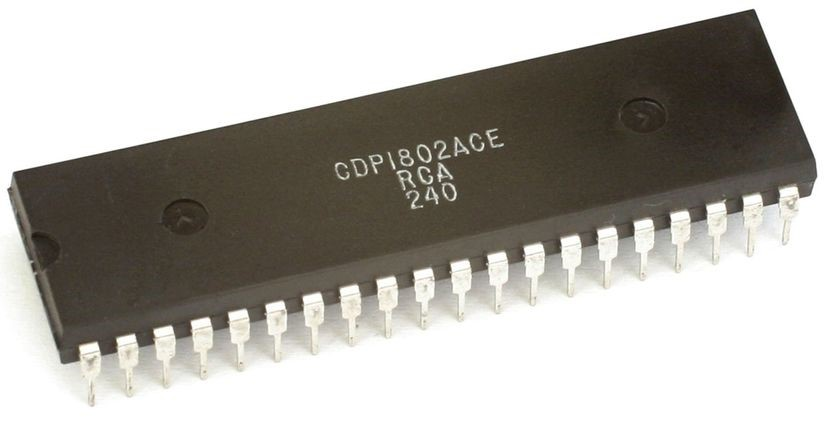
\includegraphics[width=0.5\textwidth]{./imagenes/cdp1802_encapsulado.jpg}
\caption{CDP1802 en encapsulado DIP40}
\label{F:cdp1802-encapsulado}
\end{figure}

\begin{figure}[h!]
\centering
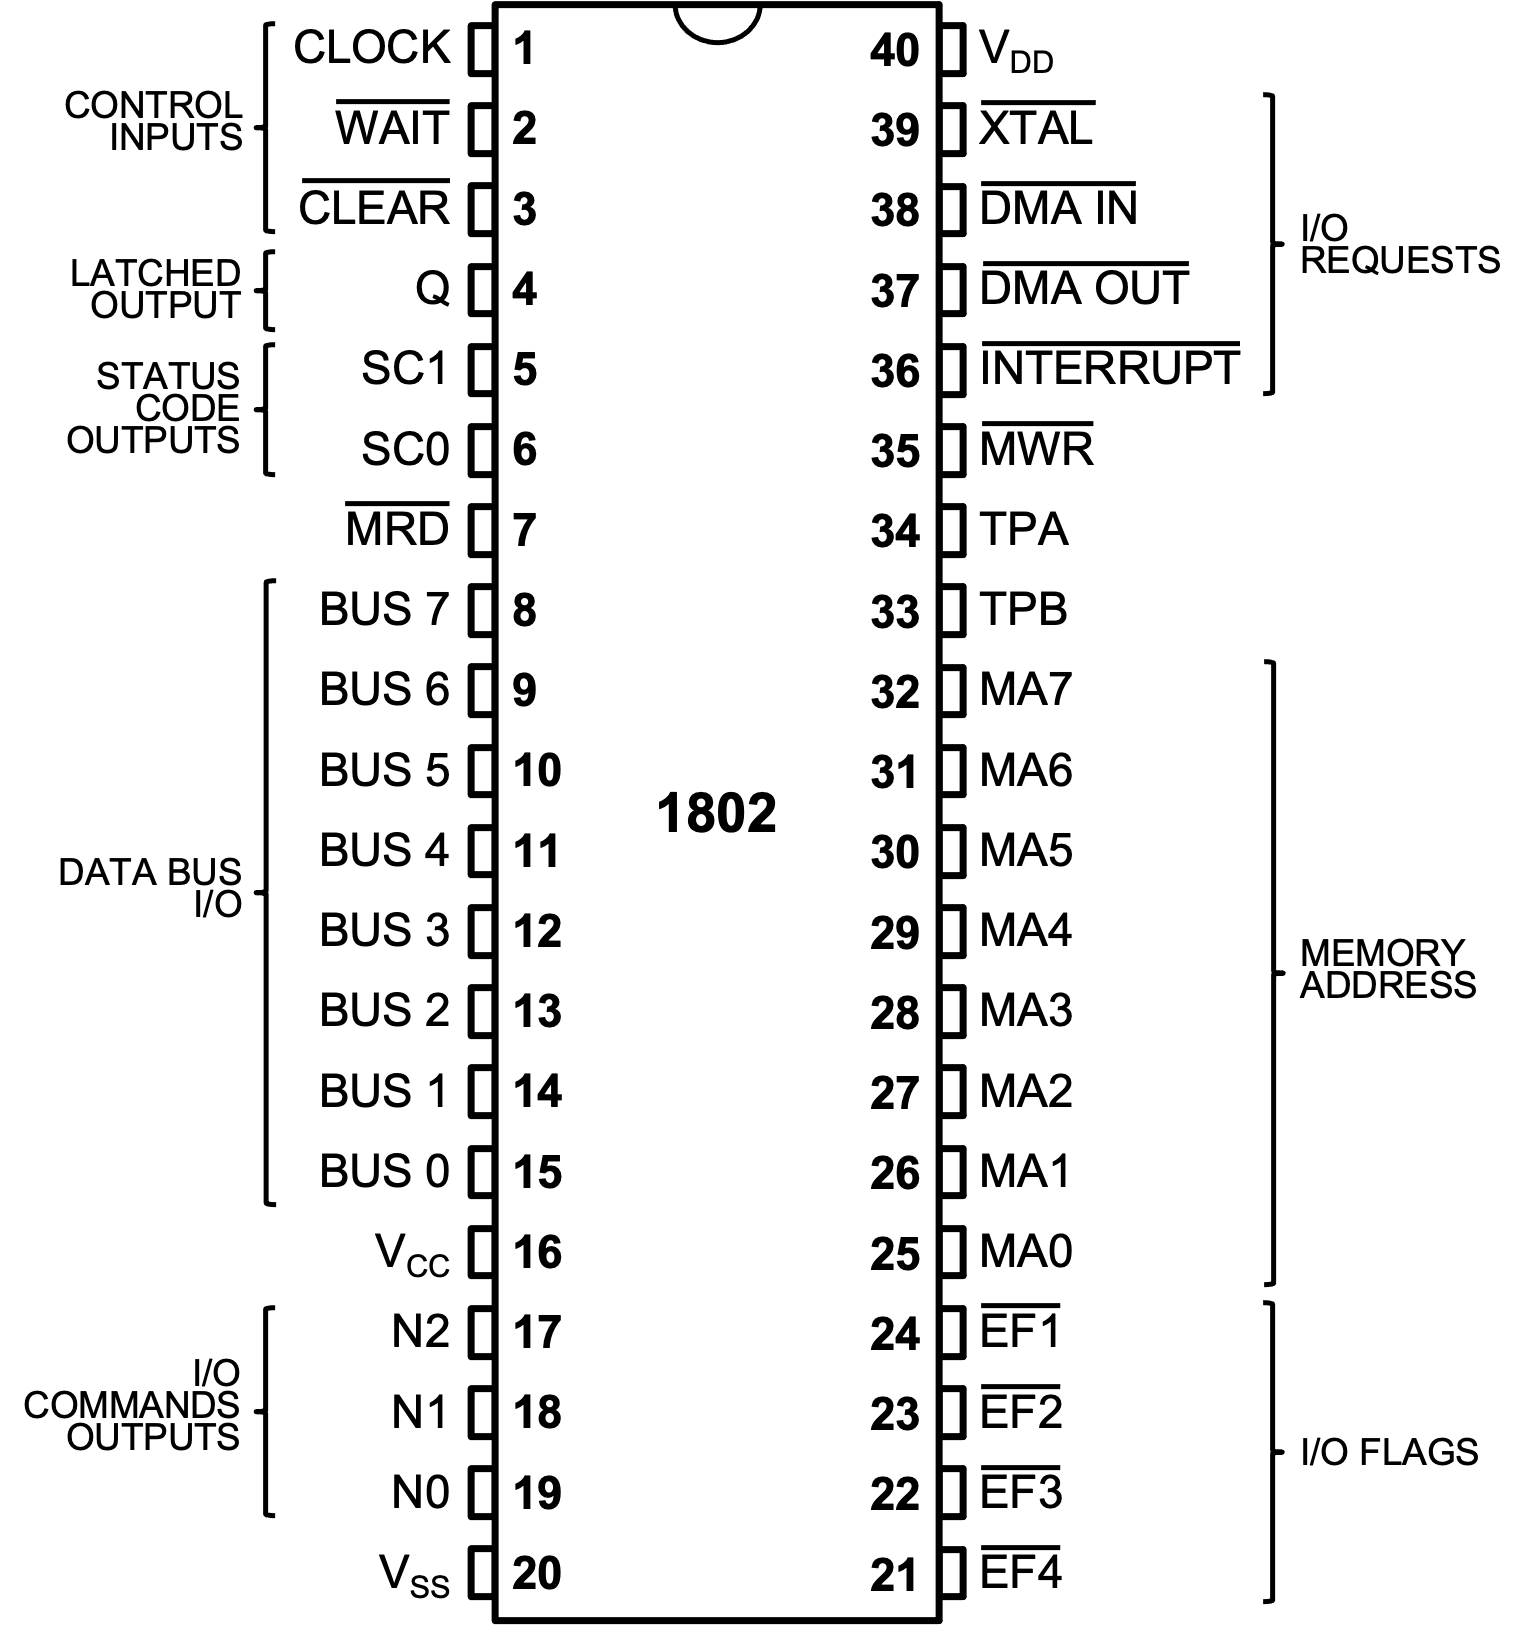
\includegraphics[width=0.65\textwidth]{./imagenes/cdp1802_pinout.png}
\caption{Distribución de pines del CDP1802}
\label{F:cdp1802-pinout}
\end{figure}

%%%%%%%%%%%%%%%%%%%%%%%%%%%%%%%%%%%%%%%%%%%%%%
\section{Computadoras basadas en el CDP1802}

\subsection{COSMAC ELF}

En la edición de agosto de 1976 de la revista Popular Electronics \cite{COSMAC_ELF_pupular_electronics}, Joseph Weisbecker detalló instrucciones para construir el COSMAC ELF basado en el CDP1802. El ELF era una computadora simplificada que permitía a los usuarios ingresar programas accionando interruptores de palanca y costaba alrededor de USD\$ 80 en partes.

\begin{figure}[h!]
\centering
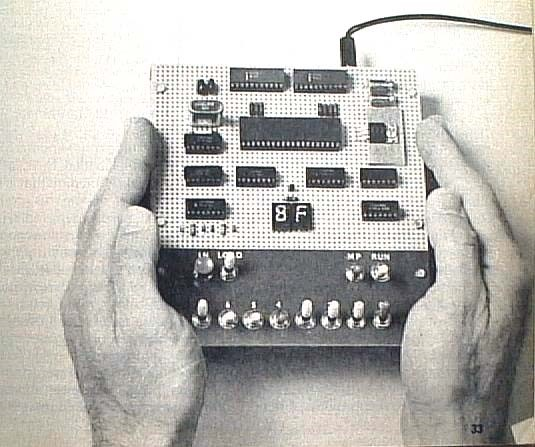
\includegraphics[width=0.7\textwidth]{./imagenes/cosmac_elf_popular_electronics.jpg}
\caption{Fotografía del COSMAC ELF de la revista Popular Electronics}
\label{F:cosmac-elf}
\end{figure}

El diseño de la computadora COSMAC ELF es simple, lo cual es así principalmente porque el CDP1802 posee un controlador DMA integrado como así también un sistema de control de dispositivos de entrada y salida, lo cual hace que no sean necesarios muchos circuitos integrados externos que de otro modo serían imprescindibles para realizar las tareas requeridas.

Una de las razones de la popularidad del CDP1802 entre los aficionados fue que su diseño facilitó la expansión de sistemas que lo utilizan y la interfaz con el mundo exterior. Los microprocesadores típicos requieren hardware de soporte y múltiples instrucciones de código máquina para utilizar periféricos de entrada y salida. Además, cuatro pines en el 1802 actúan como entradas digitales directas y con solo una instrucción de código máquina, un programa puede verificar el estado de uno de estos pines y actuar sobre el resultado. Otro pin, denominado Q, funciona como una salida de un bit que también se puede controlar con una sola instrucción de código máquina.

Una salida de un bit puede no parecer mucho, pero permite comunicación serial y el control de todo tipo de dispositivos. Tal vez lo más interesante, como señaló Weisbecker en sus artículos de Popular Electronics, es que los bucles de tiempo cuidadosamente elaborados podrían controlar con precisión la frecuencia a la que el voltaje del bit de salida cambiaba de un estado a otro, produciendo una onda cuadrada a frecuencias audibles. Esto significaba que el bit de salida podía conectarse a un altavoz y surgirían tonos musicales. Alan Turing usó una técnica similar para crear las primeras notas musicales generadas por computadora en 1951 \cite{Alan_Turing_music}.

\subsection{COSMAC ELF II}
\label{C:cosmac_elf_II}

El COSMAC ELF II es una versión mejorada de la primera COSMAC ELF, la cual incluye un teclado en lugar de interruptores para ingresar datos, además de ranuras donde pueden agregarse diferentes placas de expansión, por ejemplo, una placa de memoria RAM.

\begin{figure}[h!]
\centering
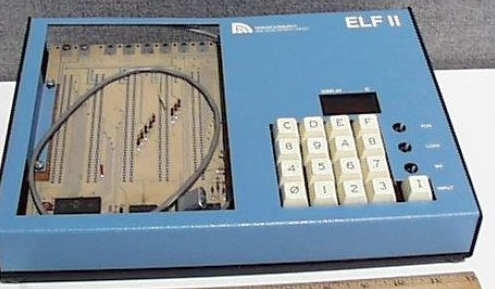
\includegraphics[width=0.7\textwidth]{./imagenes/cosmac-elf-II.png}
\caption{Fotografía obtenida en línea del COSMAC ELF II}
\label{F:cosmac-elf-II}
\end{figure}

\clearpage
\subsection{Membership Card}

La Membership Card \cite{membership-card} es una reproducción de la computadora ELF original de Popular Electronics, empaquetada para caber en una lata Altoids\textregistered~de tamaño de bolsillo. Está completamente construida con piezas y tecnología de 1980, utilizando solo componentes comunes de tecnología through hole (agujeros pasantes) y de bajo costo (sin circuitos integrados personalizados, ni componentes de montaje superficial). Para usarla no es necesario una PC moderna ni megabytes de software propietario.

\begin{figure}[ht!]
\centering
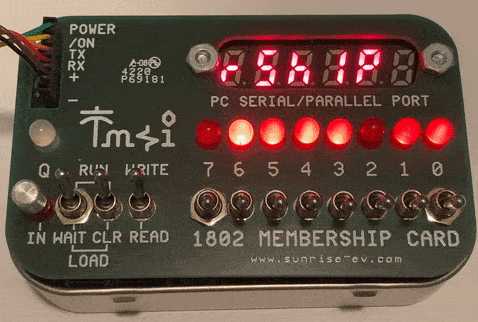
\includegraphics[width=0.6\textwidth]{./imagenes/membership-card.png}
\caption{Fotografía obtenida en línea del Membership Card}
\label{F:membership-card}
\end{figure}

La computadora está compuesta por dos placas de circuito impreso, cada una del tamaño de una tarjeta de crédito. Una es la propia Membership Card (figura~\ref{F:pcb-membership-card}), que tiene el microprocesador 1802, hasta 64k bytes de memoria, 22 bits de E/S, circuitos de reloj, reinicio, fuente de energía y además de un super-capacitor para mantener el contenido de la memoria sin energía. Se puede usar solo como un microcontrolador para proyectos como los microcontroladores Parallax BASIC Stamps o Arduino.

La segunda placa es el panel frontal (figura~\ref{F:pcb-membership-card-front-panel}). Proporciona los interruptores y los LED para un panel de control de \entreComillas{luces intermitentes}, al igual que las computadoras clásicas de antaño. Puede leer y escribir en la memoria y en los puertos de E/S manualmente, sin la ayuda de software o dispositivos externos. Los datos se muestran tanto en bits binarios individuales como en dos dígitos hexadecimales (o incluso mensajes ASCII de 6 caracteres con 4 dígitos adicionales opcionales y software apropiado).

\begin{figure}[ht!]
\centering
\subfloat[PCB Membership Card][PCB Membership Card]{
	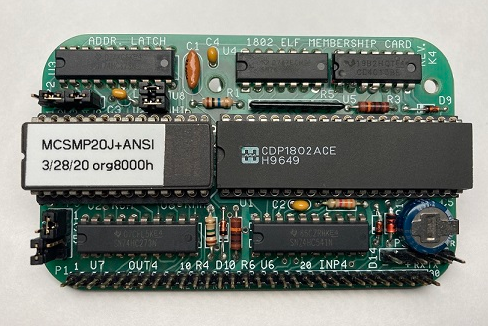
\includegraphics[width=0.6\textwidth]{./imagenes/pcb-membership-card.png}
	\label{F:pcb-membership-card}}
\\
\subfloat[PCB Membership Card Panel Frontal][PCB Membership Card Panel Frontal]{
	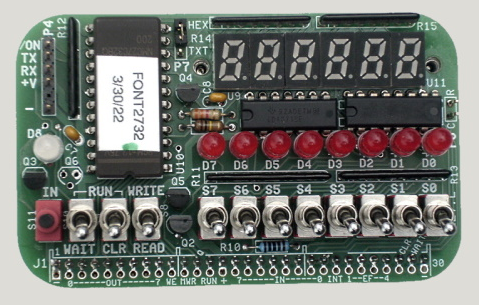
\includegraphics[width=0.6\textwidth]{./imagenes/pcb-membership-card-front-panel.png}
	\label{F:pcb-membership-card-front-panel}}
\caption{Circuitos impresos Membership Card}
\end{figure}

Un adaptador serial/USB se conecta directamente al conector de 6 pines para proporcionar alimentación y E/S serial, que permite que una terminal externa o PC cargue, guarde y ejecute programas.

\clearpage
\section{CDP1802 y la arquitectura COSMAC}

El RCA-CDP1802 es una unidad central de procesamiento (CPU) orientada a bytes que emplea la arquitectura COSMAC (Complementary Symmetry Monolithic Array Computer) y utiliza tecnología MOS (metal-oxide semiconductor) de simetría complementaria (CMOS). El microprocesador CDP1802 incluye todos los circuitos necesarios para obtener, interpretar y ejecutar instrucciones que se han almacenado en tipos estándar de memorias. También se proporcionan amplias funciones de control de entrada/salida (E/S) para facilitar el diseño del sistema.

A continuación se describen brevemente algunas características importantes del microprocesador CDP1802. La información fue obtenida del manual de usuario del mismo \cite{cdp1802_manual}.

\subsection{Características específicas}

Las funciones avanzadas y características operativas del microprocesador RCA CDP1802 incluyen:

\begin{itemize}
    \item Circuito CMOS estático, sin frecuencia de reloj mínima
    \item Rango completo de temperatura militar (-55 a +125~\unit{\degreeCelsius})
    \item Alta inmunidad al ruido y amplio rango de voltaje operativo
    \item Compatibilidad con TTL
    \item Reloj monofásico; oscilador opcional, en chip, controlado por cristal
    \item Control simple de reinicio, inicio y pausa
    \item Organización paralela de 8 bits con bus de datos bidireccional
    \item Facilidad de carga de programa incorporada
    \item Cualquier combinación de RAM y ROM estándar a través de una interfaz común
    \item Direccionamiento directo de memoria hasta 65.536 bytes
    \item Modo de E/S programable flexible
    \item Modo de interrupción del programa
    \item Recurso DMA (Direct Memory Access) en chip
    \item Cuatro entradas de bandera de E/S comprobables directamente por instrucción de salto
    \item Puertos de salida programable
    \item Formato de instrucción de uno a tres bytes con tiempo de ejecución de dos ciclos de máquina para cada instrucción\footnote{Excepto las instrucciones de saltos largos (long-branch instructions) y salteo largo (long-skip instructions) que requieren tres ciclos de máquina.}
    \item 91 instrucciones de uso simple
    \item Compatibilidad de software con el CDP1801
    \item Matriz de registros generales de 16~X~16 para usar como múltiples contadores de programa, punteros de datos o registros de datos
\end{itemize}

\subsection{Organización del sistema}

La figura~\ref{F:system_organization} ilustra un sistema informático típico que incorpora el microprocesador CDP1802. Las operaciones que se pueden realizar incluyen:

\begin{itemize}
    \item[a)] Control de dispositivos de E/S
    \item[b)] Transferencia de datos o información de control entre dispositivos de E/S y memoria
    \item[c)] Movimiento de datos entre diferentes posiciones de memoria
    \item[d)] Interpretación o modificación de bytes guardados en memoria
\end{itemize}

La memoria puede comprender cualquier combinación de RAM y ROM hasta un máximo de \num{65536}~bytes. La ROM (memoria de solo lectura) se utiliza para el almacenamiento permanente de programas, tablas y otros tipos de datos fijos. Se requiere RAM (memoria de acceso aleatorio) para los sistemas informáticos de propósito general que requieren cambios frecuentes de programa. También se requiere RAM para el almacenamiento temporal de datos variables. El tipo de memoria y la capacidad de almacenamiento requerida están determinados por la aplicación específica del sistema.

\begin{figure}[ht!]
\centering
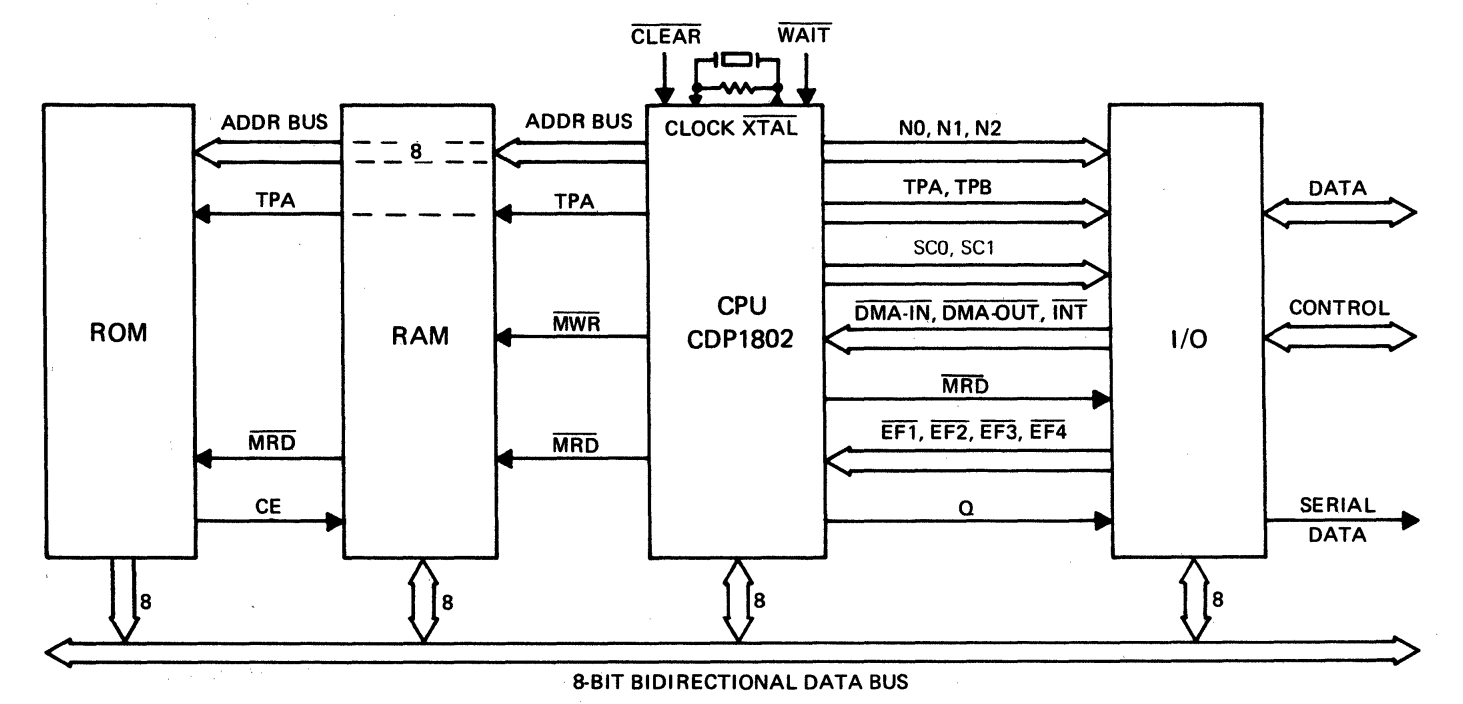
\includegraphics[width=1\textwidth]{./imagenes/system_organization.png}
\caption{\centering Diagrama de bloques de un sistema computacional típico usando el microprocesador CDP1802}
\label{F:system_organization}
\end{figure}

Los datos se transfieren desde o hacia el microprocesador entre los dispositivos de E/S y las memorias por medio de un \textbf{bus de datos bidireccional común de ocho bits} (BUS0-BUS7).

Las instrucciones de entrada/salida generan un \textbf{código N de tres bits} (N0, N1 y N2). El uso del código N para especificar un dispositivo de E/S permite un control simple y económico de una pequeña cantidad de dispositivos de E/S.

El microprocesador cuenta con \textbf{cuatro entradas que actúan como banderas de E/S} ($ \overline{\text{EF1}} $, $ \overline{\text{EF2}} $, $ \overline{\text{EF3}} $ y $ \overline{\text{EF4}} $). Los dispositivos de E/S pueden controlar estas entradas en cualquier momento para señalar al CDP1802 que se requiere una transferencia de bytes, que se ha producido una condición de error, etc. Estos indicadores también se pueden utilizar como líneas de entrada binaria si se desea. Se pueden probar mediante instrucciones CDP1802 para determinar si están activos o no.
El uso de las entradas de bandera debe coordinarse con los programas que las prueban.

También está disponible un \textbf{pin de salida} (Q), cuyo valor es controlado por instrucciones. Esta línea Q, bajo el control del programa, puede activar o señalar dispositivos de E/S. También se puede usar en conjunto con una de las entradas de bandera ($ \overline{\text{EFx}} $) para formar una interfaz de comunicación serial.

Los circuitos de E/S pueden activar una \textbf{línea de interrupción de programa} ($ \overline{\text{INT}} $) en cualquier momento para obtener una respuesta inmediata del microprocesador. La interrupción hace que el CDP1802 suspenda su secuencia de programa actual y ejecute una secuencia predeterminada de operaciones diseñadas para responder a la condición de interrupción. Después de atender la interrupción, el CDP1802 reanuda la ejecución del programa interrumpido. Se puede hacer que el CDP1802 ignore la línea de interrupción reiniciando su \textbf{flip-flop de habilitación de interrupción (IE)}.

Se proporcionan dos líneas de E/S adicionales para tipos especiales de transferencia de bytes entre la memoria y los dispositivos de E/S. Estas líneas se denominan \textbf{líneas de acceso directo a memoria} (Direct Memory Access - DMA). La activación de la línea $ \overline{\text{DMA-IN}} $ hace que un byte de entrada se almacene inmediatamente en una ubicación de memoria sin la intervención del programa que se está ejecutando. La línea $ \overline{\text{DMA-OUT}} $ hace que un byte se transfiera inmediatamente desde la memoria a los circuitos de salida solicitantes. Se utiliza un registro de puntero de memoria incorporado para indicar la ubicación de memoria para los ciclos de DMA. El programa establece inicialmente este puntero en una ubicación de memoria inicial. Cada transferencia de byte DMA incrementa automáticamente el puntero a la siguiente ubicación de memoria. La activación repetida de una línea DMA puede provocar la transferencia de cualquier número de bytes consecutivos hacia y desde la memoria, independientemente de la ejecución simultánea del programa.

Los circuitos de dispositivos de E/S pueden provocar la transferencia de datos al activar una línea de bandera ($ \overline{\text{EFx}} $), la línea de interrupción ($ \overline{\text{INT}} $) o una línea DMA ($ \overline{\text{DMA-IN}} $ o $ \overline{\text{DMA-OUT}} $). El programa debe muestrear las líneas de bandera para determinar cuándo se activan y se utilizan para detectar señales relativamente lentas. La activación de la línea de interrupción provoca una respuesta inmediata, independientemente del programa que se esté ejecutando actualmente, suspendiendo la operación de ese programa y permitiendo una respuesta en tiempo real. El uso de DMA proporciona la respuesta más rápida con la menor perturbación del programa.

Se proporciona un \textbf{código de estado de dos bits} (SC0 y SC1) y \textbf{dos líneas de temporización} (TPA y TPB) para que los utilicen los circuitos de dispositivos de E/S. Estas cuatro señales permiten la sincronización de circuitos de E/S con ciclos operativos internos del CDP1802. El código de estado indica si el CDP1802 está respondiendo a una solicitud de DMA, respondiendo a una solicitud de interrupción, obteniendo una instrucción o ejecutando una instrucción; esto se encuentra resumido en la tabla~\ref{T:state_codes}. Los sistemas de memoria y de E/S utilizan las señales de temporización para señalar un nuevo código de estado del procesador, bloquear bits de dirección de memoria (para obtener direccionamiento de hasta 16 bits con solo 8 pines de dirección), tomar datos de memoria del bus y establecer o restablecer los flip-flops del controlador de E/S.

% Please add the following required packages to your document preamble:
% \usepackage{multirow}
\begin{table}[ht!]
\caption{Códigos de estado}
\label{T:state_codes}
\begin{tabular}{|l|ll|}
\hline
\multicolumn{1}{|c|}{\multirow{2}{*}{State Type}} & \multicolumn{2}{l|}{State Code} \\ \cline{2-3} 
\multicolumn{1}{|c|}{}                            & \multicolumn{1}{l|}{SC1}  & SC0 \\ \hline
S0 (Fetch)                                        & \multicolumn{1}{l|}{L}    & L   \\ \hline
S1 (Execute)                                      & \multicolumn{1}{l|}{L}    & H   \\ \hline
S2 (DMA)                                          & \multicolumn{1}{l|}{H}    & L   \\ \hline
S3 (Interrupt)                                    & \multicolumn{1}{l|}{H}    & H   \\ \hline
\end{tabular}
\end{table}

El CDP1802 proporciona ocho líneas de dirección de memoria (MA0-MA7). Estas ocho líneas proporcionan direcciones de memoria de 16 bits en forma de dos bytes de 8 bits sucesivos. El byte de dirección más significativo (de orden superior) aparece primero en las ocho líneas de dirección, seguido del byte de dirección menos significativo (de orden inferior). El número de bits de orden superior necesarios para seleccionar una ubicación de byte de memoria única depende del tamaño de la memoria. Por ejemplo, una memoria de 4096 bytes requeriría una dirección de 12 bits. Esta dirección de 12 bits se obtiene combinando 4 bits del byte de dirección de orden superior con los 8 bits del byte de dirección de orden inferior. Uno de los dos pulsos de temporización del CDP1802 se puede usar para introducir los bits de orden superior requeridos en un latch de dirección (registro paralelo de 8 bits) cuando aparecen en las ocho líneas de dirección.

Cuatro líneas adicionales completan la interfaz del sistema del microprocesador. Una entrada de reloj monofásica (CLOCK) determina la velocidad de funcionamiento. El reloj externo se puede detener y comenzar nuevamente, continuando con la operación del CDP1802 donde se había quedado antes de detenerse el reloj. La construcción del circuito de reloj se simplifica mediante el uso de la entrada $ \overline{\text{XTAL}} $. Se conecta un cristal entre $ \overline{\text{XTAL}} $ y la entrada de reloj CLOCK, por lo cual no se necesitan componentes activos. La línea de entrada $ \overline{\text{CLEAR}} $ inicializa el microprocesador y su liberación inicia la ejecución de las instrucciones. La línea $ \overline{\text{WAIT}} $ suspende la operación de la CPU limpiamente. La activación simultánea de $ \overline{\text{CLEAR}} $ y $ \overline{\text{WAIT}} $ pone a la CPU en un modo de carga de programa. La tabla~\ref{T:CDP1802_modes} resume estos modos de operación.

\begin{table}[ht!]
\caption{Modos del CDP1802}
\label{T:CDP1802_modes}
\begin{tabular}{|l|l|l|}
\hline
      &      & \\
$ \overline{\text{CLEAR}} $ & $ \overline{\text{WAIT}} $ & MODE  \\[0.3cm] \hline
L     & L    & Load  \\
L     & H    & Reset \\
H     & L    & Pause \\
H     & H    & Run   \\ \hline
\end{tabular}
\end{table}

\subsection{Notación de la arquitectura COSMAC}

La figura~\ref{F:estructura_interna} ilustra la estructura interna del microprocesador COSMAC CDP1802. Esta arquitectura se basa en una matriz de registros que comprende dieciséis registros tipo \textbf{scratch-pad} de 16 bits de propósito general. Cada registro (denominados \textbf{R}) se designa mediante un código binario de 4 bits. Aquí se utilizará la \textbf{notación hexadecimal (hex)} para referirse a códigos binarios de 4 bits; en la tabla~\ref{T:dec_bin_hex} se encuentra el equivalente decimal y binario de todos los dígitos hexadecimales.
Siguiendo la notación hexadecimal, podemos referirnos a los registros 3 y 12 como \textbf{R(3)} y \textbf{R(C)}, respectivamente. De esta manera nos referimos a los registros de 16~bits; sin embargo, podemos referirnos a los bytes que lo componen como \textbf{R(3).0} y \textbf{R(3).1}, que indican el byte menos significativo y más significativo de \textbf{R(3)}, respectivamente.

\begin{figure}[ht!]
\centering
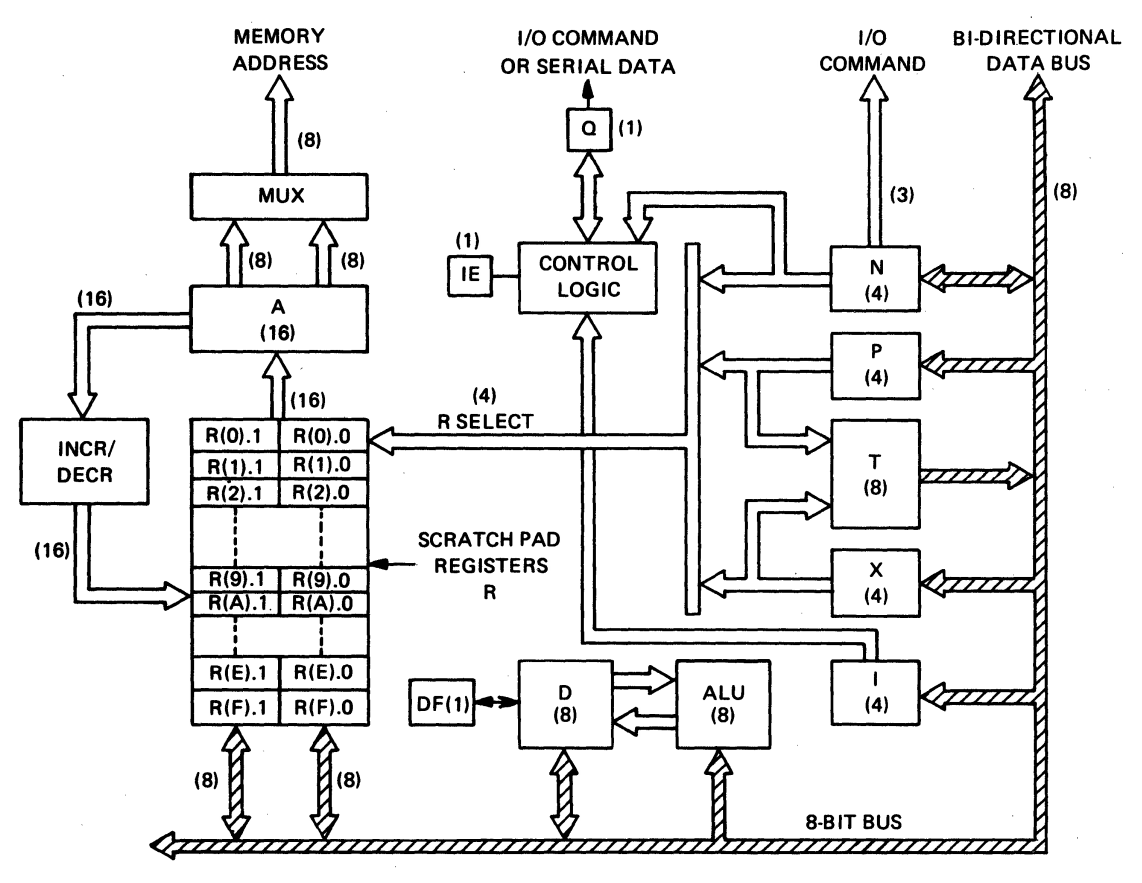
\includegraphics[width=1\textwidth]{./imagenes/estructura_interna.png}
\caption{Estructura interna del microprocesador CDP1802}
\label{F:estructura_interna}
\end{figure}

\begin{table}[ht!]
\caption{Numeración decimal, binaria y hexadecimal}
\label{T:dec_bin_hex}
\begin{tabular}{|c|c|c|}
\hline
Decimal & Binario & Hexadecimal \\ \hline \hline
0       & 0000    & 0           \\ \hline
1       & 0001    & 1           \\ \hline
2       & 0010    & 2           \\ \hline
3       & 0011    & 3           \\ \hline
4       & 0100    & 4           \\ \hline
5       & 0101    & 5           \\ \hline
6       & 0110    & 6           \\ \hline
7       & 0111    & 7           \\ \hline
8       & 1000    & 8           \\ \hline
9       & 1001    & 9           \\ \hline
10      & 1010    & A           \\ \hline
11      & 1011    & B           \\ \hline
12      & 1100    & C           \\ \hline
13      & 1101    & D           \\ \hline
14      & 1110    & E           \\ \hline
15      & 1111    & F           \\ \hline
\end{tabular}
\end{table}

Tres registros de 4 bits denominados \textbf{N}, \textbf{P} y \textbf{X} contienen los códigos binarios de 4 bits (dígitos hexadecimales) que se utilizan para seleccionar registros de 16~bits individualmente. La notación \textbf{R(X)}, \textbf{R(N)} o \textbf{R(P)} se usa para referirse a un registro de 16~bits seleccionado por el código de 4 bits en \textbf{X}, \textbf{N} o \textbf{P}, respectivamente.

De esta manera, la siguiente notación denota que la parte baja de \textbf{R(N)} es transferida al registro de 8~bits \textbf{D}, que es similar al acumulador encontrado comúnmente en microprocesadores, y el bit \textbf{DF} es el Carry de \textbf{D}, y el mismo pasa a \entreComillas{1} si el resultado de una operación desborda \textbf{D}.

\begin{equation*}
    \text{ R(N).0 } \rightarrow \text{ D }
\end{equation*}

También se puede leer directamente de la memoria utilizando uno de los registros de trabajo de 16 bits para realizar el direccionamiento para la lectura, como se muestra en la siguiente notación.

\begin{equation*}
    \text{ M(R(X)) } \rightarrow \text{ D }
\end{equation*}

El flip-flop interno \textbf{Q} se puede configurar o restablecer mediante instrucciones, y también existen instrucciones de salto condicional en base al valor de \textbf{Q}. El estado de \textbf{Q} también está disponible como salida del microprocesador.

\paragraph{Formato de instrucciones}

La operación del microprocesador se especifica mediante una secuencia de códigos de instrucción almacenados en la memoria externa. Se aplica un formato de instrucción de un byte para la mayoría de las instrucciones. Los dos dígitos hexadecimales de 4~bits que componen cada byte de instrucción se designan como \textbf{I} y \textbf{N}, como se muestra en la figura~\ref{F:instruction_format}.

\begin{figure}[ht!]
\centering
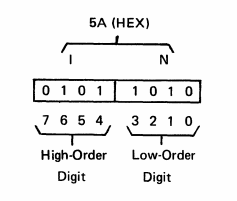
\includegraphics[width=0.35\textwidth]{./imagenes/instruction_format.png}
\caption{Formato de instrucción}
\label{F:instruction_format}
\end{figure}

Para la mayoría de las instrucciones, la ejecución requiere dos ciclos máquina. El primer ciclo (Fetch Cycle) lee el byte de instrucción apropiado de la memoria y almacena los dos dígitos de instrucción hexadecimales en los registros internos \textbf{I} y \textbf{N}. Los valores en \textbf{I} y \textbf{N} especifican la operación que se realizará durante el segundo ciclo máquina. \textbf{I} especifica el tipo de instrucción. Según la instrucción, \textbf{N} designa un registro de trabajo o, en otros casos, actúa como un código especial.

Las instrucciones normalmente se ejecutan en secuencia. Se utiliza un contador de programa para direccionar sucesivamente los bytes de memoria que representan las instrucciones. En la arquitectura COSMAC, cualquiera de los registros de trabajo general de 16~bits puede ser utilizado como contador de programa. El valor del dígito hexadecimal contenido en el registro \textbf{P} determina qué registro de trabajo se está utilizando actualmente como contador de programa. Las operaciones realizadas por el ciclo de búsqueda (Fetch Cycle) se representan de la siguiente manera.

\begin{equation*}
    \text{ M(R(P)) } \rightarrow \text{ I,N ; R(P)+1} \rightarrow \text{ R(P) }
\end{equation*}

\paragraph{Contadores de programa múltiples}

Un contador de programa es un registro que apunta a la siguiente instrucción a buscar y ejecutar. La arquitectura COSMAC brinda la capacidad única de especificar, en una sola instrucción (instrucción SEP), cualquiera de los 16 registros de trabajo como contador de programa. Esta característica hace posible mantener punteros a varios programas diferentes simultáneamente y transferir el control rápidamente de uno a otro. Un puntero a un programa que atiende una solicitud de interrupción, o la posibilidad de crear subrutinas que pueden operar sin RAM, son solo dos ejemplos de esta función.


\chapter{Programas utilizados}

\section{Entorno de programación - Visual Studio Code}

Existen muchos entornos de programación disponibles, el utilizado para el proyecto fue Visual Studio Code \cite{visual_studio_code}. El mismo fue utilizado porque es gratuito y se encuentra disponible para Windows, Linux y Mac.

Visual Studio Code es un entorno de desarrollo flexible que cuenta con extensiones que pueden ser instaladas para ayudar con la escritura y visualización de código. En la figura~\ref{F:vsc_extensions} se encuentran capturas de pantalla del entorno de programación, indicando con flechas numeradas la secuencia para encontrar las dos extensiones utilizadas.

\begin{figure}[ht!]
\centering
\subfloat[Extensión para visualización en Assembler]{
	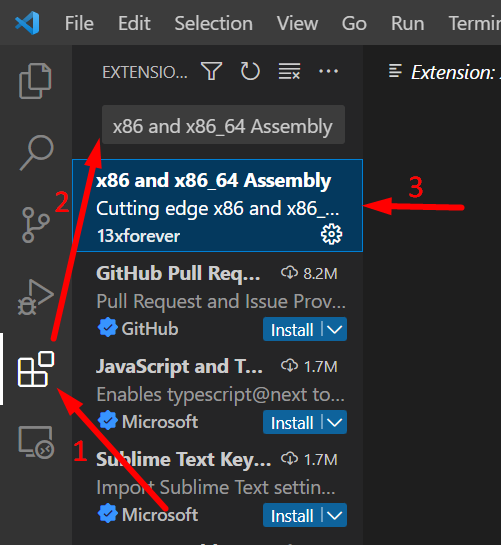
\includegraphics[width=0.4275\textwidth]{./imagenes/vsc_assembly_ext.png}
	\label{F:vsc_assembly_ext}}
\quad
\subfloat[Extensión para visualización de formato Intel]{
	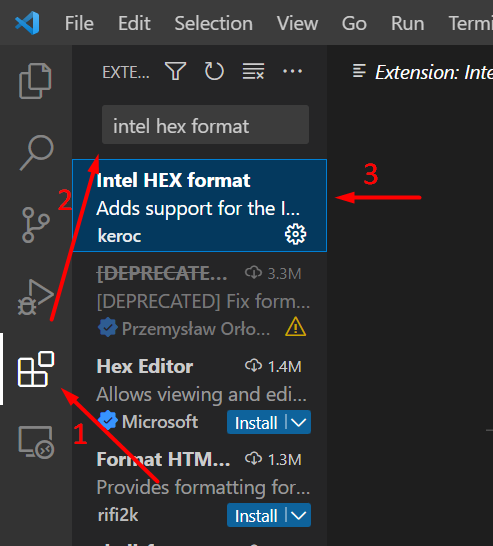
\includegraphics[width=0.42275\textwidth]{./imagenes/vsc_intel_ext.png}
	\label{F:vsc_intel_ext}}
\caption{Extensiones utilizadas en Visual Studio Code}
\label{F:vsc_extensions}
\end{figure}

La primera de ellas, \entreComillas{x86 and x86\_64 Assembly}, es una extensión para el resaltado de sintaxis. En la figura~\ref{F:snyntax_highlighting} puede apreciarse un programa sencillo que hace parpadear el LED Q en un sistema con el CDP1802, donde lo más importante es la diferencia de color entre las instrucciones y los comentarios, lo cual facilita la lectura y análisis del código.

\begin{figure}[ht!]
  \centering
  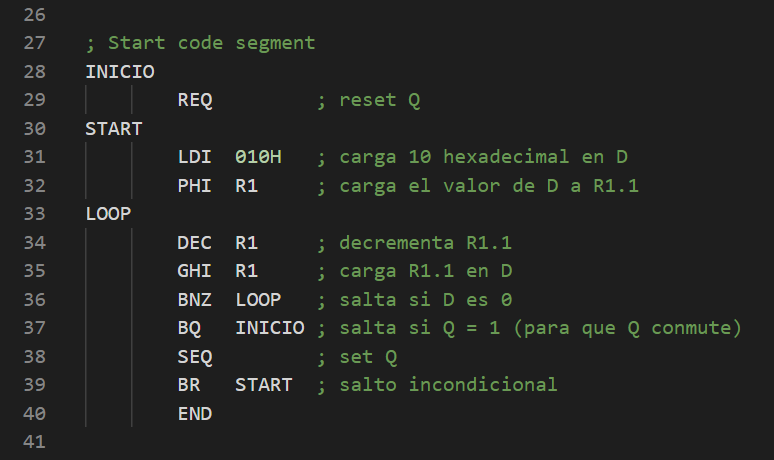
\includegraphics[width=.75\textwidth]{./imagenes/syntax highlishtpng.png}
  \caption{Extensión para resaltar sintaxis de código en assembler}
  \label{F:snyntax_highlighting}
\end{figure}

La segunda extensión es \entreComillas{Intel HEX format}, dedicada a resaltar la composición de archivos en formato Intel, lo cual sería difícil de otro modo, o requeriría un programa específico para esta tarea. En la figura~\ref{F:intel_highlighting} se encuentra una captura de pantalla de un archivo Intel visualizado con esta extensión. En el anexo~\ref{C:anexo_formato_intel} (\nameref{C:anexo_formato_intel}) se encuentra descrito el formato Intel.

\begin{figure}[ht!]
  \centering
  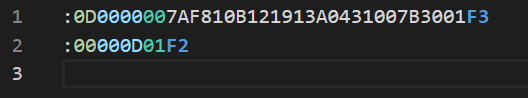
\includegraphics[width=0.57\textwidth]{./imagenes/intel_format_highlighting.png}
  \caption{Extensión para resaltar la composición de archivos en formato Intel}
  \label{F:intel_highlighting}
\end{figure}

\section{Revisión de modificaciones con Git y Visual Studio Code}

Cuando se tienen programas grandes y se sabe que se han realizado modificaciones, intentar encontrarlas y ver nada más estos cambios puede resultar una tarea engorrosa. Sin embargo, existen herramientas para poder visualizar cambios realizados en un código. Una de estas herramientas es Git, un programa para llevar el control de versión del desarrollo de código. Git es un programa con muchas funciones, pero la única que es de interés en este momento es la revisión de diferencias entre dos archivos.

Para utilizar esta herramienta primero debe descargarse Git desde \cite{git_download}, y una vez instalado se requiere una pequeña configuración, la cual puede verse en el video tutorial \cite{git_difftool_config}, pero de igual manera se describe a continuación.

Primero debe abrirse Git, para ello debe hacerse click derecho en una parte vacía de un directorio cualquiera, también puede ser el escritorio, y hacer click en \entreComillas{Git Bash Here}, como puede verse en la figura~\ref{F:git_inst_1}. Luego, en la ventana del programa, escribir los comandos como se muestran en la figura~\ref{F:git_inst_2}.

\begin{figure}[ht!]
\centering
\subfloat[Abrir Git]{
	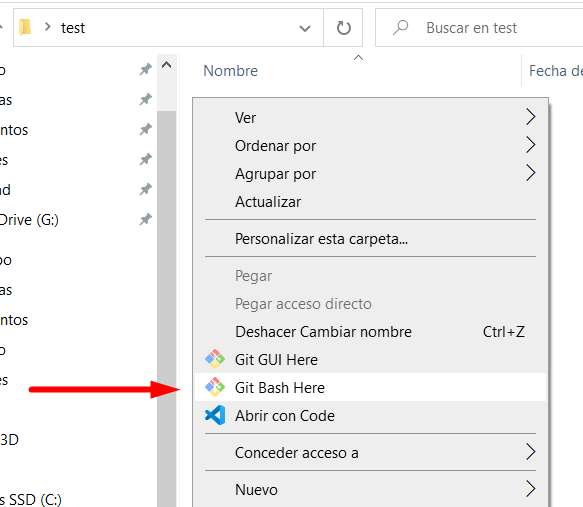
\includegraphics[width=0.57\textwidth]{./imagenes/git_inst_1.png}
	\label{F:git_inst_1}}
\\
\subfloat[Comandos para la configuración inicial]{
	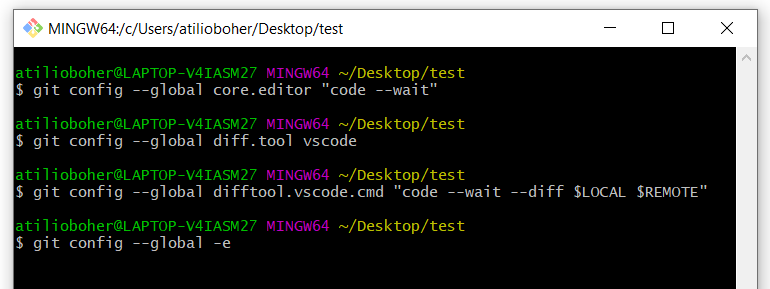
\includegraphics[width=0.8\textwidth]{./imagenes/git_inst_2.png}
	\label{F:git_inst_2}}
\caption{Configuración inicial de Git}
\label{F:git_inst}
\end{figure}

Al ejecutar el último comando, Visual Studio Code se abrirá, y la configuración realizada debería verse como en la figura~\ref{F:git_inst_3}, de no ser así, debe rellenarse lo faltante, guardar el archivo y cerrar el programa.

\begin{figure}[ht!]
  \centering
  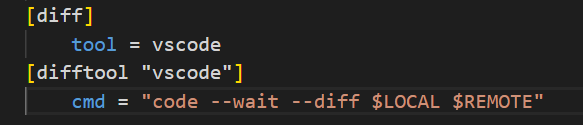
\includegraphics[width=0.57\textwidth]{./imagenes/git_inst_3.png}
  \caption{Configuración de Git relacionada a difftool}
  \label{F:git_inst_3}
\end{figure}

Una vez hecho todo esto, Git se encuentra configurado y se pueden comparar dos archivos simplemente abriendo Git, como ya se indicó en la figura~\ref{F:git_inst_1}, y escribiendo el comando que se observa en la captura de la figura~\ref{F:git_inst_4}, donde los dos últimos parámetros son los nombres de los archivos a comparar (en este caso \texttt{test.asm} y \texttt{test\_modificado.asm}).

\begin{figure}[ht!]
  \centering
  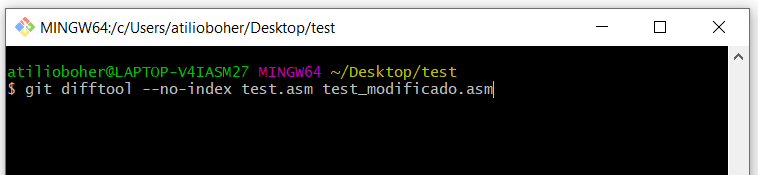
\includegraphics[width=0.8\textwidth]{./imagenes/git_inst_4.png}
  \caption{Comando para comparar dos archivos con Git}
  \label{F:git_inst_4}
\end{figure}

En la figura~\ref{F:git_difftool_exemple} puede apreciarse la diferencia entre los códigos, en este caso es una simple diferencia ilustrativa.

\begin{figure}[ht!]
  \centering
  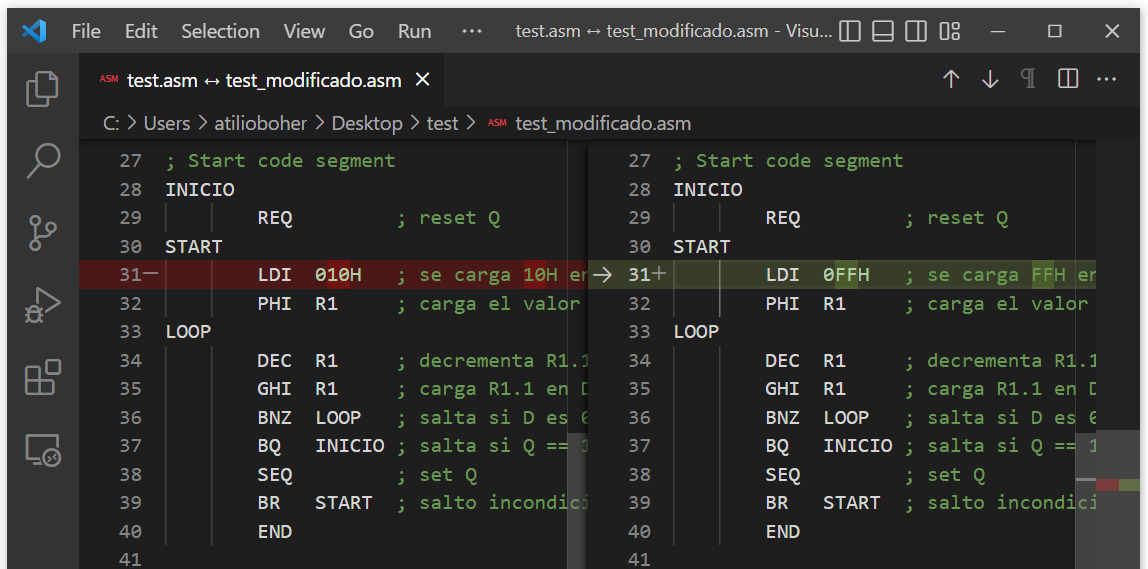
\includegraphics[width=0.99\textwidth]{./imagenes/git_difftool_exemple.png}
  \caption{Ejemplo de comparación}
  \label{F:git_difftool_exemple}
\end{figure}

Lo útil de esta herramienta es que no solo indica la línea, sino también el lugar exacto del cambio o diferencia.

\section{Ensamblador A18}
\label{C:a18}

El ensamblador utilizado se denomina A18 y fue encontrado en \cite{a18} donde se encuentra el enlace para poder descargarlo. Con el mismo es posible ensamblar código assembler del CDP1802 (con los mnemónicos indicados en su hoja de datos \cite{cdp1802_datasheet}) y obtener los archivos en formato Intel (\texttt{.hex}) y el listing (\texttt{.lst}). Además cuenta con un manual donde se indica cómo utilizarlo y todos los tipos de errores que pueden encontrarse a la hora de realizar el ensamblado.

Para utilizarlo es necesario tener el archivo \texttt{a18.exe} en el mismo directorio que el código \texttt{.asm} que busca ensamblarse. Luego, manteniendo apretado Shift izquierdo, se debe hacer click en una parte vacía del directorio y luego seleccionar \entreComillas{Abrir la ventana de PowerShell aquí}, como se aprecia en la figura~\ref{F:a18_1} (es posible que en vez de PowerShell diga Command Prompt, cualquiera sea el caso, se prosigue de la misma manera), esto abre una ventana de comandos en el directorio en cuestión.

\begin{figure}[ht!]
  \centering
  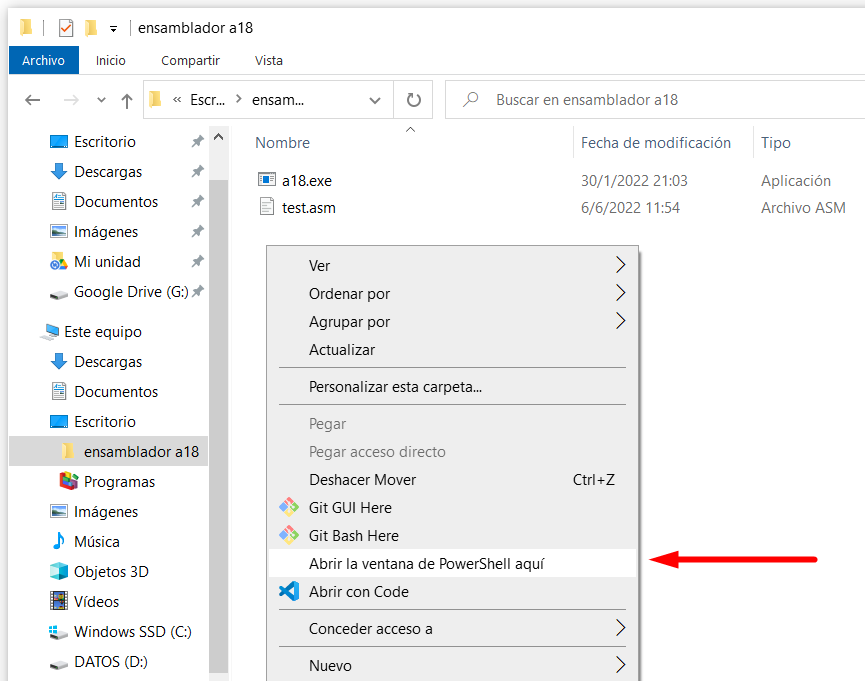
\includegraphics[width=0.75\textwidth]{./imagenes/a18_1.png}
  \caption{Apertura de ventana de comandos en directorio}
  \label{F:a18_1}
\end{figure}

En la ventana de comandos se deben reemplazar los nombres correspondientes; el primero es el nombre del programa a ensamblar, en formato \texttt{.asm}, el segundo es el nombre del archivo \texttt{.hex} a generar, y el último es el nombre del archivo listing, en formato \texttt{.lst}.

\vspace{0.75cm}
\footnotesize
\texttt{./a18.exe <nombre-de-archivo>.asm -o <nombre-de-archivo>.hex -l <nombre-de-archivo>.lst}
\normalsize
\vspace{0.75cm}

En la figura~\ref{F:a18_2} puede verse el resultado del ensamblado de un programa y si el mismo posee errores, es indicado al ejecutar el comando. En el archivo listing generado se encuentran indicadas las líneas que poseen errores, utilizando un código para identificar cada tipo de error, de manera que los detalles sobre los mismos pueden ser encontrados en el manual del ensamblador, que como ya se mencionó, puede encontrarse en la página \cite{a18}.

\begin{figure}[ht!]
  \centering
  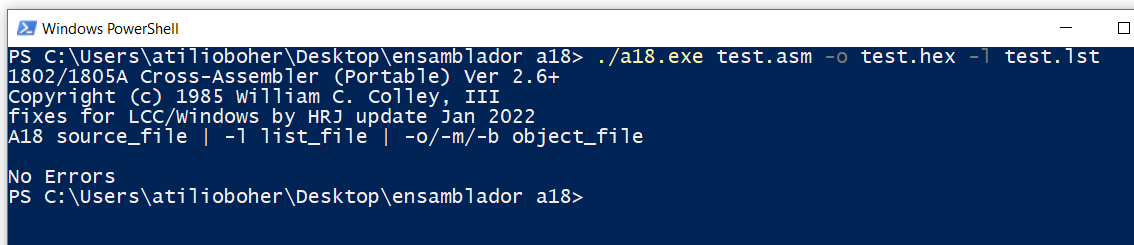
\includegraphics[width=0.95\textwidth]{./imagenes/a18_2.png}
  \caption{Resultado del ensamblado en ventana de comandos}
  \label{F:a18_2}
\end{figure}

Escribir este comando puede resultar engorroso. Por lo cual se escribió un pequeño script Batch, cuyas instrucciones se encuentran en la figura~\ref{F:a18_3}. Este script Batch se puede ejecutar con doble click y ensambla el código. Para ello el archivo Batch \texttt{.bat} debe tener el mismo nombre que el archivo \texttt{.asm} a ensamblar. En la figura~\ref{F:a18_4} se encuentra una captura de pantalla de los archivos necesarios, al hacer doble click en \texttt{test.bat}, se abrirá una ventana de comandos y \texttt{test.asm} se ensamblará automáticamente, sin necesidad de escribir ningún comando.

\begin{figure}[ht!]
\centering
\subfloat[Instrucciones Batch para el ensamblado con doble click]{
	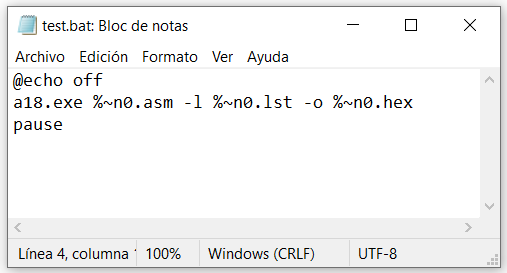
\includegraphics[width=0.47\textwidth]{./imagenes/a18_3.png}
	\label{F:a18_3}}
\quad
\subfloat[Uso del archivo \texttt{.bat}]{
	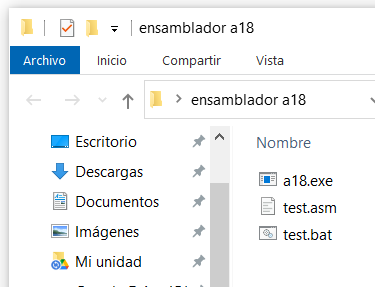
\includegraphics[width=0.39\textwidth]{./imagenes/a18_4.png}
	\label{F:a18_4}}
\caption{Ensamblado con script Batch}
\label{F:a18_5}
\end{figure}

\clearpage
\section{Emulador Emma02}

Existe un software llamado Emma02, el cual puede encontrarse en su página oficial \cite{emma_02}. El mismo permite la simulación de varios modelos de computadoras basadas en el microprocesador CDP1802. En la figura~\ref{F:emma02_interfas} puede apreciarse la variedad de computadoras disponibles, sin embargo, la más utilizada fue el Membership Card, seguida del Netronics Elf II.

\begin{figure}[ht!]
  \centering
  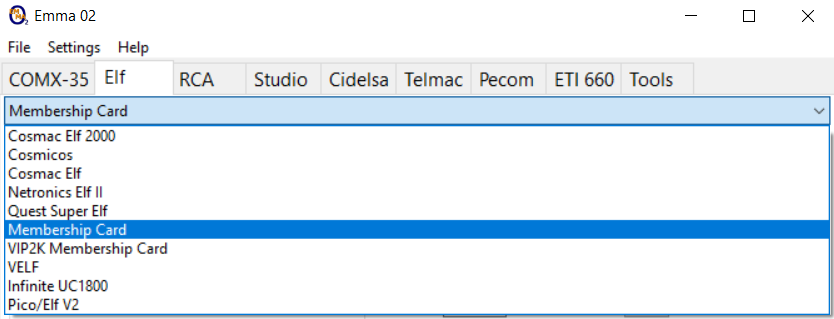
\includegraphics[width=0.85\textwidth]{./imagenes/emma02_interfaz.png}
  \caption{Computadoras disponibles que utilizan el CDP1802}
  \label{F:emma02_interfas}
\end{figure}

El simulador cuenta con programas ya disponibles para cada computadora. Para utilizar uno, debemos seleccionarlo en la solapa que se indica en la figura~\ref{F:emma02_1}; pero hay que tener en cuenta que quizás requiera cambiar alguna configuración de la computadora, como seleccionar la velocidad de transmisión correcta, el mapa de memoria, la dirección donde el microprocesador comenzará a ejecutar el programa, etc.

\begin{figure}[ht!]
  \centering
  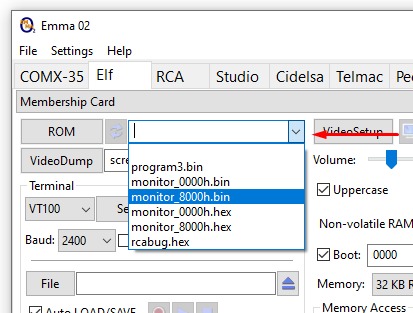
\includegraphics[width=0.5\textwidth]{./imagenes/emma02_1.png}
  \caption{Seleccionar programa}
  \label{F:emma02_1}
\end{figure}

Además, existe una forma de seleccionar programas ya disponibles en el simulador junto a la configuración específica necesaria para su funcionamiento, para ello hay que ir a File->Configuration->Load, como se indica en la figura~\ref{F:emma02_2}, para el caso de la computadora Netronics~Elf~II.

\begin{figure}[ht!]
  \centering
  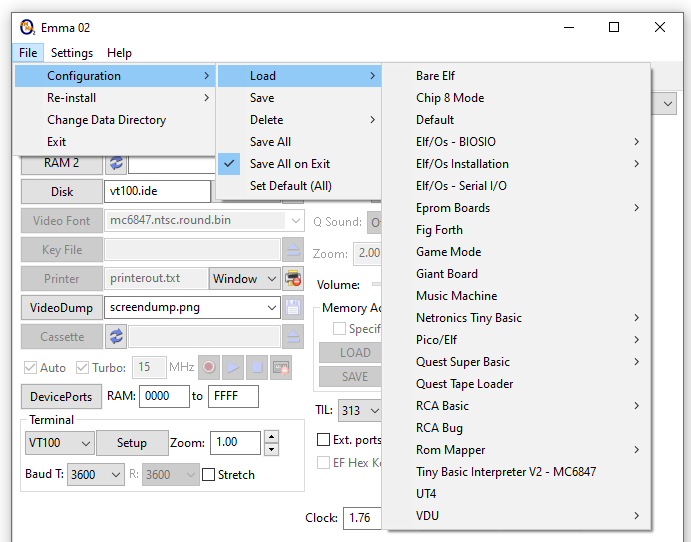
\includegraphics[width=0.89\textwidth]{./imagenes/emma02_2.png}
  \caption{Seleccionar programa y configuración}
  \label{F:emma02_2}
\end{figure}

Algunos de estos programas se encuentran en formato \texttt{.bin} y otros en formato \texttt{.hex}. Además, algunos también poseen el código fuente \texttt{.asm} en la carpeta contenedora. Para acceder a esta carpeta podemos hacer click en \entreComillas{ROM}, como se indica en la figura~\ref{F:emma02_ROM}. Esto abrirá una ventana para seleccionar un archivo \texttt{.hex} o \texttt{.bin}, y en esta ventana puede verse el directorio del emulador donde se encuentran los programas disponibles.

En este directorio (hay uno por cada modelo de computadora) pueden agregarse programas obtenidos en línea, o escritos y ensamblados por uno mismo para ser probados.

\begin{figure}[ht!]
  \centering
  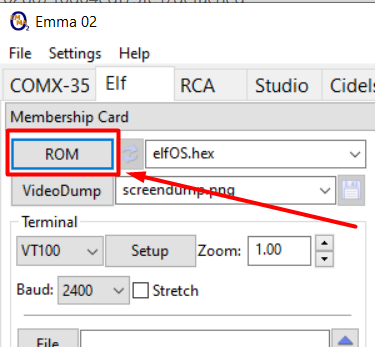
\includegraphics[width=0.37\textwidth]{./imagenes/emma02_cargar_hex.png}
  \caption{Seleccionar programa en Emma02}
  \label{F:emma02_ROM}
\end{figure}

El emulador también provee una herramienta denominada \entreComillas{Direct Assembler} (ver figura~\ref{F:emma02_direct_asm}), la cual muestra el código del programa en lenguaje assembler; puede ensamblar y desensamblar. Sin embargo, en este proyecto, se utilizó únicamente como herramienta de depuración de código y para el ensamblado se utilizó el ensamblador A18, ya expuesto en la sección~\ref{C:a18}.

\begin{figure}[ht!]
  \centering
  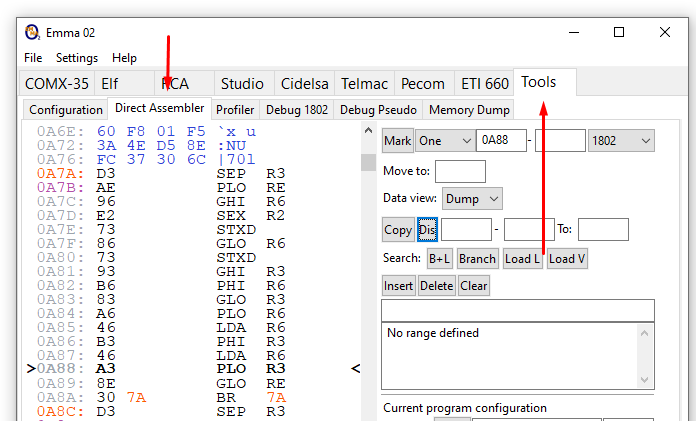
\includegraphics[width=0.8\textwidth]{./imagenes/emma02_direct_asm.png}
  \caption{Direct Assembler}
  \label{F:emma02_direct_asm}
\end{figure}

También existe una pestaña donde puede visualizarse los registros internos del microprocesador, y haciendo click en el botón \entreComillas{Trace} (figura~\ref{F:emma02_trace}), se registran todas las instrucciones ejecutadas, pudiendo luego copiar y pegar esto en un documento de texto para analizar detenidamente la ejecución de una secuencia de código.

\begin{figure}[ht!]
  \centering
  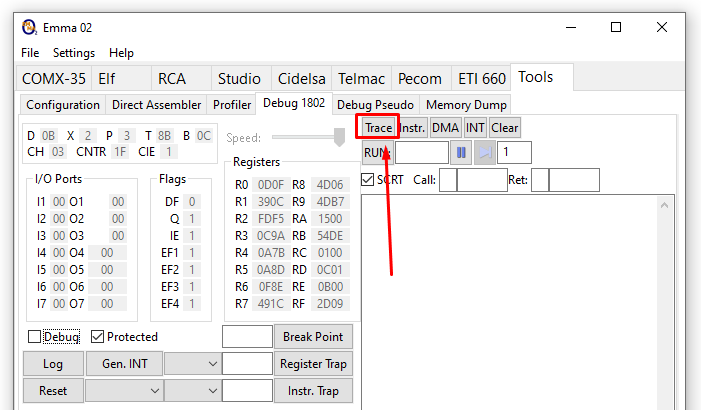
\includegraphics[width=0.8\textwidth]{./imagenes/emma02_trace.png}
  \caption{Registrar instrucciones ejecutadas y visualización de Registros internos}
  \label{F:emma02_trace}
\end{figure}

En la figura~\ref{F:emma02_trace_1} se encuentra una captura de instrucciones registradas con la herramienta \entreComillas{Trace}, en rojo se marcó una instrucción de escritura en memoria como ejemplo para ver cómo puede visualizarse información de interés, en este caso, tanto la dirección de memoria que fue escrita como el dato escrito en ella.

\begin{figure}[ht!]
  \centering
  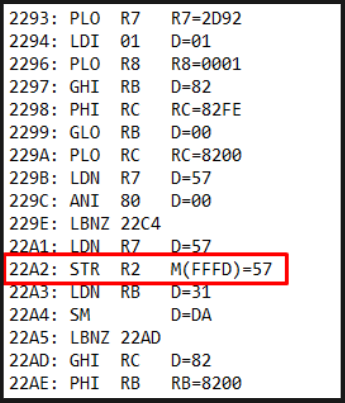
\includegraphics[width=0.38\textwidth]{./imagenes/emma02_trace_1.png}
  \caption{Captura de instrucciones ejecutadas}
  \label{F:emma02_trace_1}
\end{figure}

Estas características y herramientas mencionadas fueron las más utilizadas, sin embargo, se encuentran descritos más detalles de estas herramientas y otras más en la sección de ayuda de la página del emulador \cite{emma_02_help}.

\clearpage
\section{Terminal Tera Term}

Para la comunicación con la computadora se utiliza una terminal externa, en este caso se utilizó el programa Tera Term\copyright\cite{teraterm} ejecutándose en un ordenador personal. El mismo es sencillo de usar, sin embargo, se mencionan algunas configuraciones que se hicieron para volver más fácil su uso.

En la figura~\ref{F:teraterm_font} se puede ver la configuración realizada para tener un tamaño de letra más grande, debido a que la configuración por defecto es muy chica. Esta ventana de configuración puede encontrarse en Setup->Font->Font...

\begin{figure}[ht!]
  \centering
  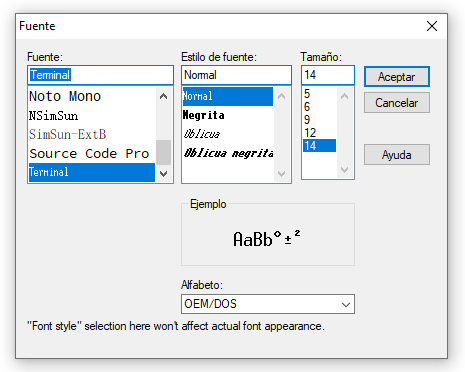
\includegraphics[width=0.6\textwidth]{./imagenes/teraterm_font.png}
  \caption{Tamaño y tipo de letra de la terminal}
  \label{F:teraterm_font}
\end{figure}

La configuración realizada se pierde cada vez que el programa es cerrado, por lo tanto, cada vez que se abre el mismo debería realizarse la misma configuración nuevamente. Para evitar esto es posible guardar la configuración actual, para ello es necesario ir a Setup->Save setup..., una ventana se abrirá y podrá guardarse un archivo llamado \entreComillas{TERATERM.INI}, guardarlo reescribe la configuración anterior, por lo tanto, si no desea perderla, debería guardar el archivo de configuración ya existente antes de sobrescribirlo.

Algunos programas pueden ser cargados desde la terminal. Esto es usado, por ejemplo, para cargar programas escritos en Basic, al intérprete de Basic corriendo en el microprocesador, el cual es discutido en el capítulo~\ref{C:SistemaMedio}: \nameref{C:SistemaMedio}, sección~\ref{C:programas_del_sistema_medio}: \nameref{C:programas_del_sistema_medio}.

Para realizar esta tarea se tiene que ir a File->Send file... y seleccionar el archivo que contiene el programa a ser enviado a través de la terminal (ver figura~\ref{F:teraterm_send_file}). Como el microprocesador requiere de un período de tiempo mínimo para poder procesar un carácter recibido, no es posible enviarlos todos de seguido sin establecer un retardo entre cada uno de ellos; por esta razón Tera Term posee una configuración para esto en Setup->Serial port..., en la ventana de configuración pueden configurarse los retardos entre caracteres y líneas; en la figura~\ref{F:teraterm_transmit_delay} se indica dónde colocar estos valores.

\begin{figure}[H]
\centering
\subfloat[Opción de envío de archivo]{
	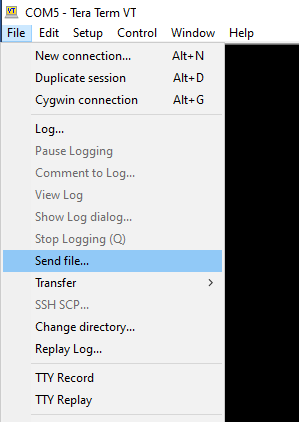
\includegraphics[width=0.35\textwidth]{./imagenes/teraterm_send_file.png}
	\label{F:teraterm_send_file}}
\quad
\subfloat[Configuración de delay]{
	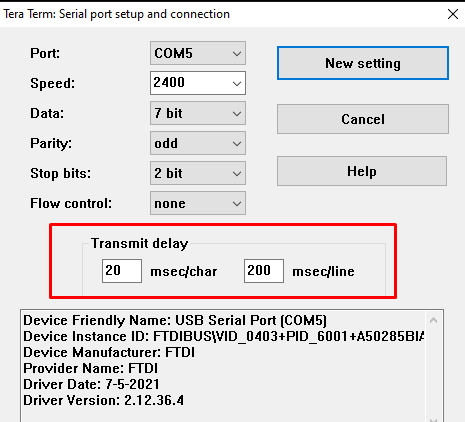
\includegraphics[width=0.45\textwidth]{./imagenes/teraterm_transmit_delay.png}
	\label{F:teraterm_transmit_delay}}
\caption{Cargado de programas a través de la terminal}
\label{F:send_file}
\end{figure}

Para que este proceso funcione correctamente debe respetarse el carácter ASCII utilizado para representar un salto de línea. Dado que distintos formatos de texto utilizan diferentes caracteres para esto (algunos utilizan retorno de carro CR, del inglés \textit{Carriage Return}, o salto de línea LF, del inglés \textit{Line Feed}). Estos no necesariamente son los que el programa ejecutándose en el microprocesador interpreta como salto de línea, a veces es necesario modificarlos. Para ello se utilizó el programa discutido en la siguiente sección, \nameref{C:multicomander}.

\section{Multi Commander}
\label{C:multicomander}

Multi Commander \cite{multicommander} es un programa para el manejo de archivos y se utiliza como alternativa al explorador de Windows. Sin embargo, es de interés para este proyecto únicamente la herramienta para cambiar los caracteres utilizados para representar saltos de línea en archivos de texto. En la figura~\ref{F:multicommander} se puede observar dónde encontrar esta herramienta dentro del programa.

\begin{figure}[H]
  \centering
  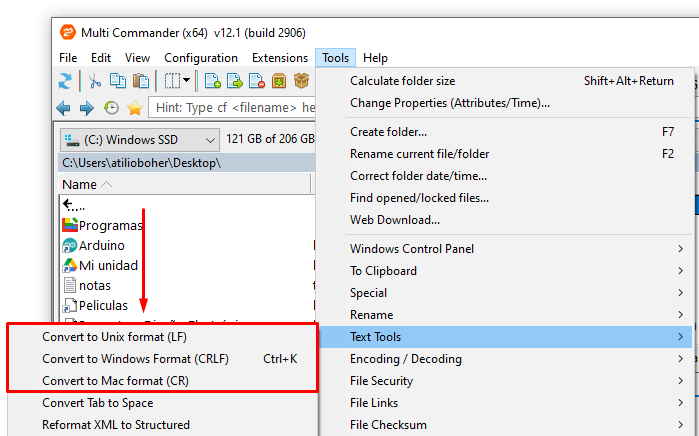
\includegraphics[width=0.85\textwidth]{./imagenes/multicommander.png}
  \caption{Herramienta para cambio de carácter de salto de línea en Multi Commander}
  \label{F:multicommander}
\end{figure}


\section{Programador universal XGecu TL866-3G}
\label{C:Programador}

Para el grabado de la memoria se utilizó el programador universal XGecu TL866-3G (figura~\ref{F:programador_universal}). Para ello fue necesaria la descarga e instalación del software correspondiente al mismo, el cual puede ser encontrado en la página oficial del fabricante \cite{pagina_de_descarga_programador}. Se recomienda descargar la opción 2 \entreComillas{DownLoad From Local Server}.

\begin{figure}[ht!]
  \centering
  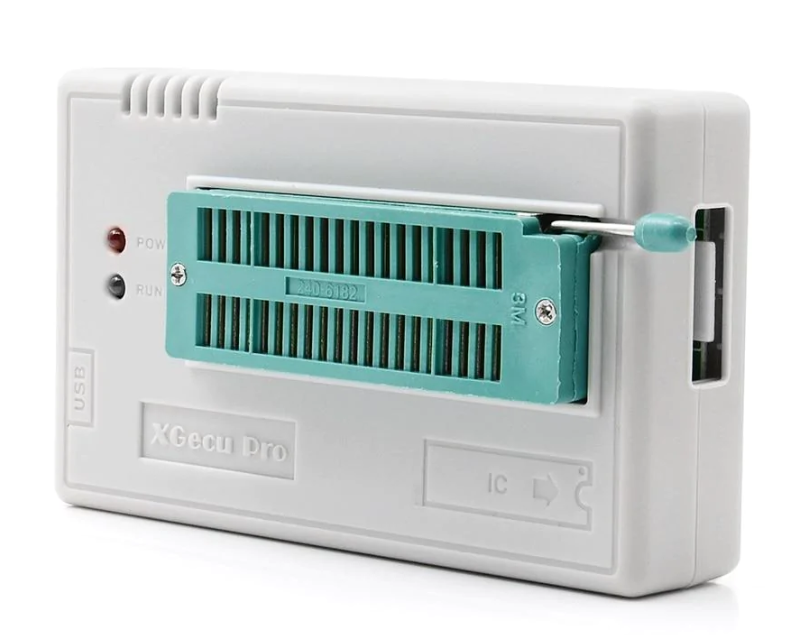
\includegraphics[width=0.6\textwidth]{./imagenes/programador_universal.png}
  \caption{Programador universal XGecu TL866-3G}
  \label{F:programador_universal}
\end{figure}

En la figura~\ref{F:programador_universal_opciones} puede verse el entorno gráfico del programa. Con la flecha~1 se encuentra indicado donde seleccionar la memoria a ser grabada o leída. En este proyecto fueron utilizadas las memorias AT28C64\cite{datasheet_AT28C64} y X28C256\cite{datasheet_X28C256}, ambas disponibles en la librería del programador. Con la flecha~2 se indica una función para el testeo de chips lógicos digitales, herramienta que fue de utilidad en varias ocasiones.

\begin{figure}[ht!]
  \centering
  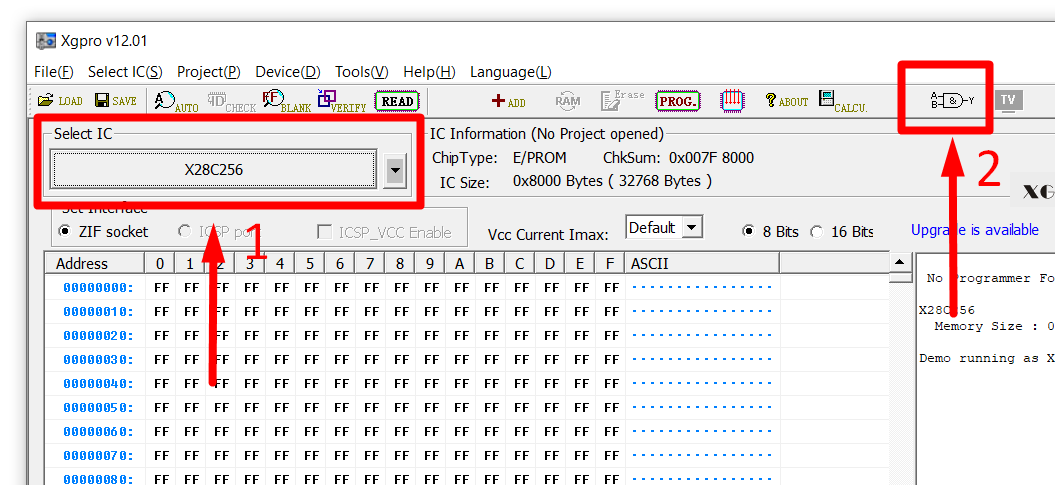
\includegraphics[width=0.85\textwidth]{./imagenes/programador_universal_opciones.png}
  \caption{Entorno gráfico del programa del programador universal XGecu TL866-3G}
  \label{F:programador_universal_opciones}
\end{figure}

\clearpage
\section{KiCad EDA}

Para la construcción de los circuitos electrónicos del presente proyecto se utilizó el software KiCad, un software libre para el diseño electrónico automatizado (del inglés: Electronic Design Automation EDA) de circuitos electrónicos. 
Entre las aplicaciones más destacadas del software se encuentran:  el editor de esquemas, el editor de circuitos impresos y el selector de huellas impresas para los componentes utilizados, entre otras. 
KiCad es un software de código abierto y gratuito, el cual puede ser descargado de su página oficial \cite{kicad_page}. En línea pueden encontrarse video-tutoriales muy completos para el uso adecuado del mismo.
La versatilidad de la herramienta mencionada ha proporcionado simpleza al momento de confeccionar los esquemáticos y los diagramas de circuito impreso para las placas del proyecto. A modo de ejemplo en las figuras~\ref{F:esquema_kikad} y~\ref{F:pcb_kikad} se encuentran el editor de esquemas y el editor de circuitos impresos del software KiCad. 

\begin{figure}[ht!]
  \centering
  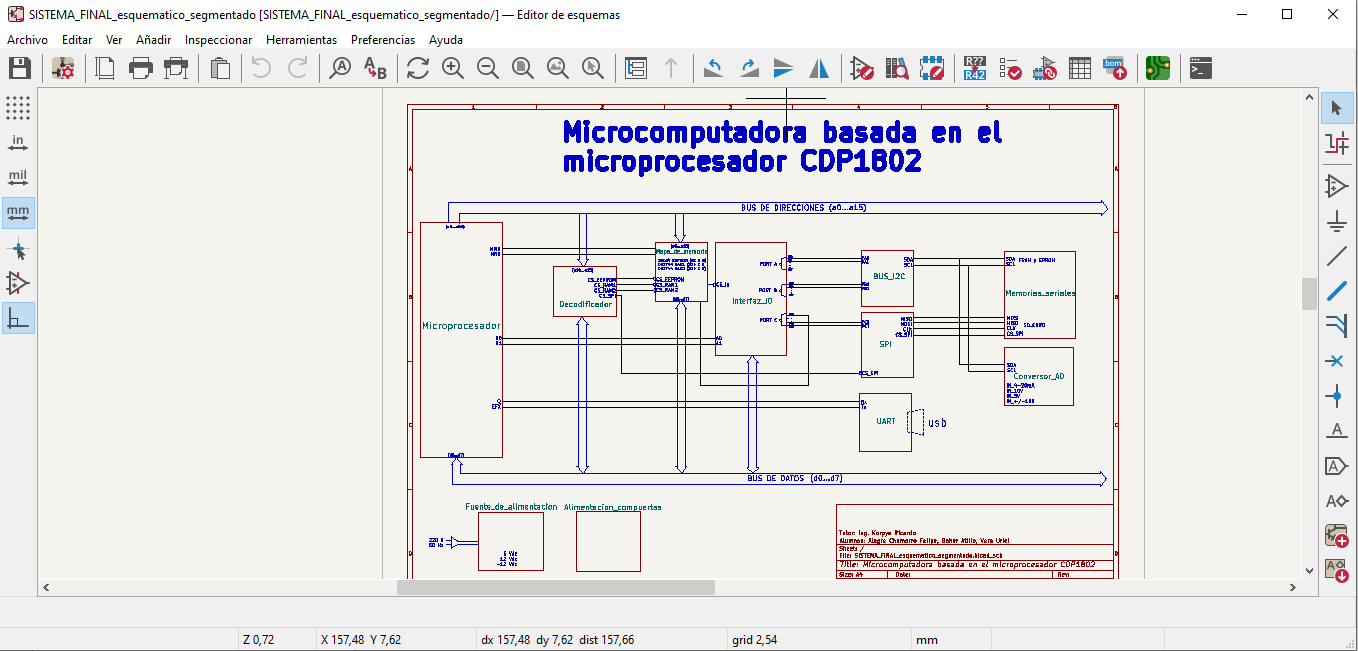
\includegraphics[width=0.95\textwidth]{./imagenes/esquema_kikad.png}
  \caption{Entorno gráfico del editor de esquemas del software KiCad}
  \label{F:esquema_kikad}
\end{figure}

Una herramienta destacada para el diseño de los circuitos impresos es el editor de huellas y de símbolos, lo cual es útil a la hora de confeccionar un esquemático o un PCB cuando se posee un dispositivo cuyo símbolo o huella no está incluida dentro de las librerías del programa. KiCad cuenta con un entorno adecuado para el dibujo y desarrollo de los elementos mencionados, permitiendo agregar a las librerías los mismos. Esta solución realza la aplicabilidad del programa y ha sido de gran utilidad para el desarrollo del trabajo.

\begin{figure}[ht!]
  \centering
  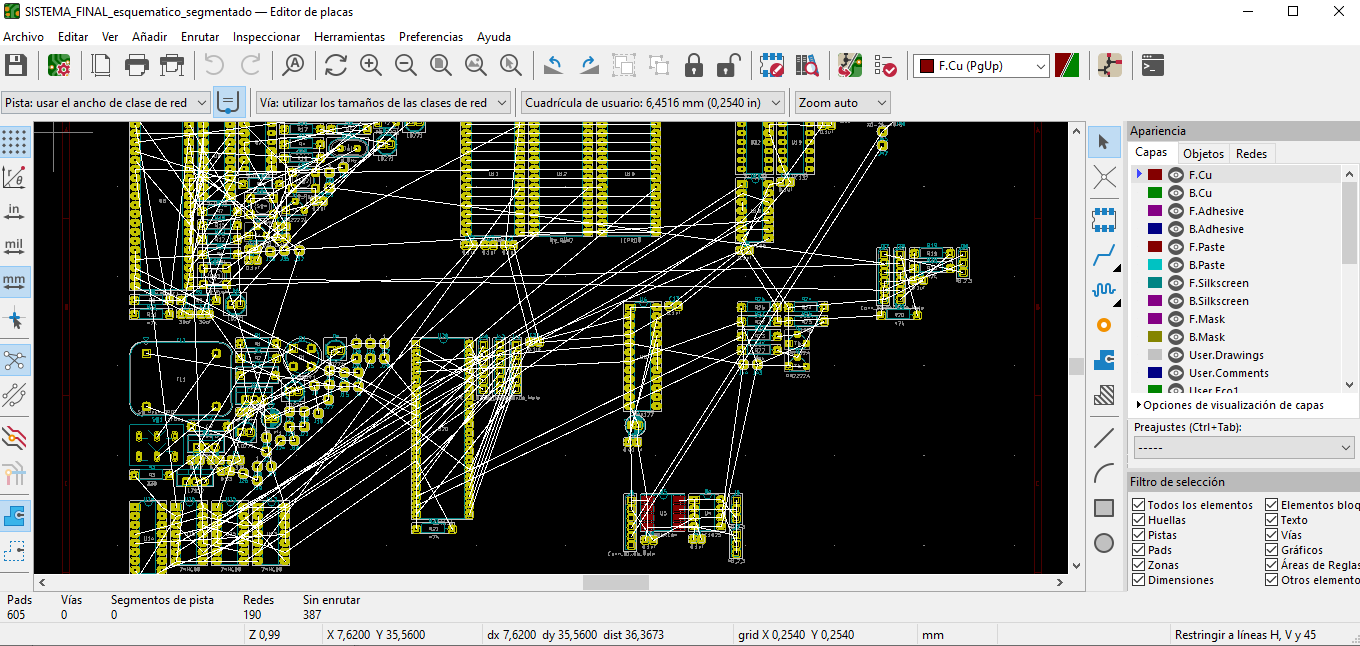
\includegraphics[width=0.95\textwidth]{./imagenes/pcb_kikad.png}
  \caption{Entorno gráfico del editor de circuito impreso del software KiCad}
  \label{F:pcb_kikad}
\end{figure}
% --------------------
  \chapter{Pruebas en el COSMAC ELF II}
% --------------------
\label{C:pruebas_cosmac_elf_II}

%%%%%%%%%%%%%%%%%%%%%%%%%%%%%%%
En las instalaciones de la facultad de ingeniería se cuenta con el COSMAC ELF II, el cual fue comentado en la sección~\ref{C:cosmac_elf_II}. A modo de introducción, antes de comenzar a desarrollar los sistemas del proyecto, se realizaron pruebas sobre el COSMAC ELF II, para probar su funcionamiento y comenzar a comprender la operación del microprocesador. 

\begin{foto}[ht!]
  \centering
  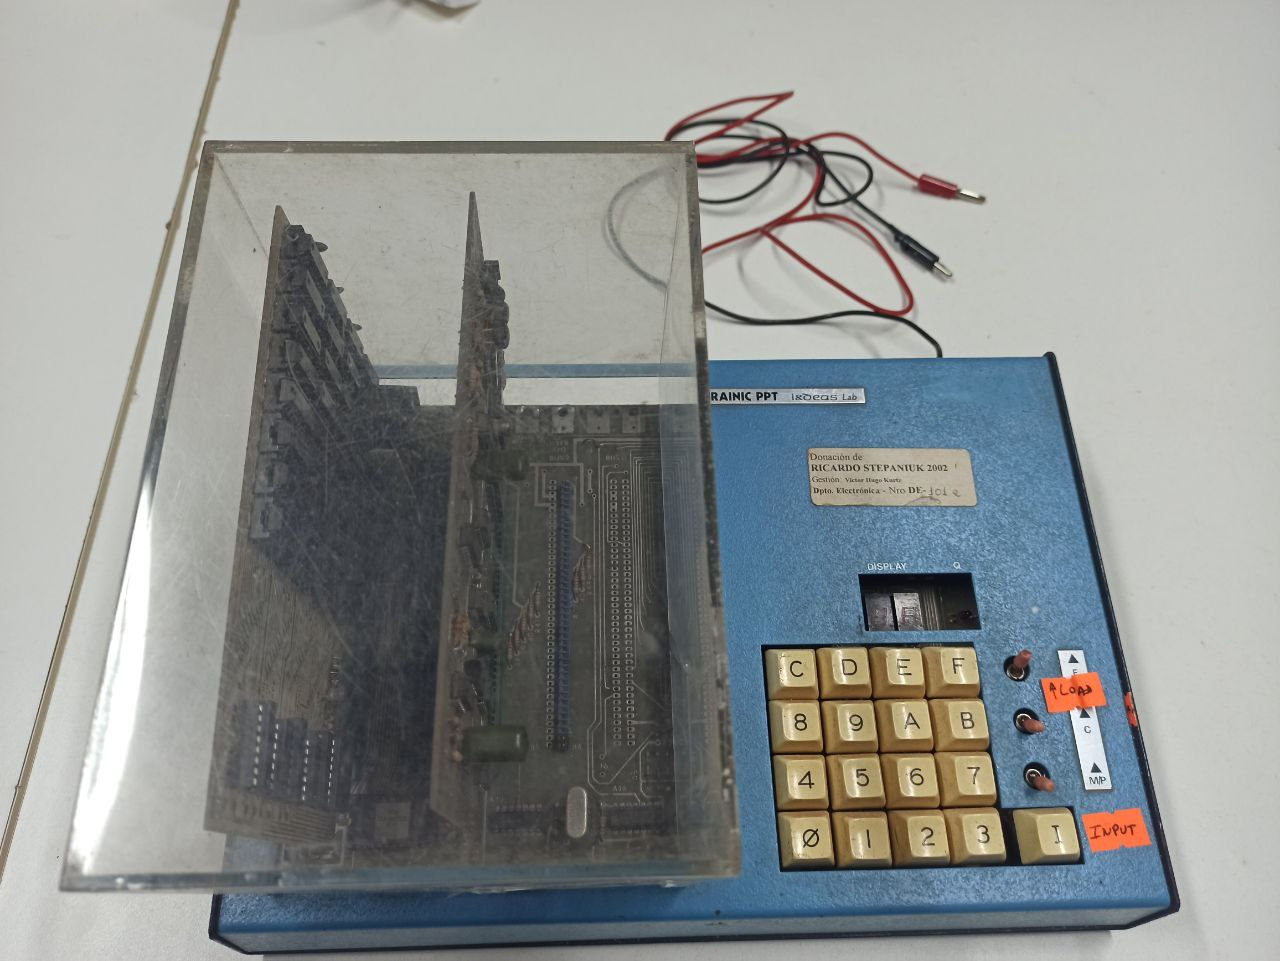
\includegraphics[width=.9\textwidth]{./imagenes/cosmac_elf_II_facu.jpg}
  \caption{COSMAC ELF II, propiedad de la facultad de ingeniería}
  \label{F:cosmac_elf_ii_falcultad}
\end{foto}

En la figura~\ref{F:cosmac_elf_ii_falcultad} se encuentra una fotografía del COSMAC ELF II que se encuentra en la facultad. Para utilizarlo fue necesario realizar reparaciones sobre el mismo. Un capacitor de entrada en la etapa de alimentación (en paralelo al pin de entrada del regulador LM7805) se encontraba dañado y fue necesario reemplazar el mismo, como así también soldar un cable a la placa para reemplazar una pista que se encontraba dañada. Luego se soldaron dos cables a los pines de alimentación de la placa de la computadora, para así poder conectarla a una fuente de alimentación.

Una vez realizadas estas reparaciones, se conectó el COSMAC ELF II a una fuente de alimentación configurada a \num{8}~\si{\volt} y se encendió. Para comprobar su funcionamiento correcto, se grabaron dos programas encontrados en línea \cite{programacion_cosmac}, junto con la explicación detallada del procedimiento para realizar la programación.

Se puede cargar un programa en el COSMAC ELF II poniendo el interruptor LOAD en la posición ON, con RUN y MP (Memory Protect) en OFF, y luego ingresar un byte con el teclado para finalmente presionar el botón INPUT. Esto graba un byte en la primera dirección de memoria. Para grabar otro byte en la siguiente dirección de memoria simplemente se debe ingresar el mismo en el teclado y volver a presionar INPUT. Una vez que se ingresaron todos los bytes del programa, MP debe colocarse en ON para proteger la memoria.

Con el programa ya cargado, para correrlo, se debe colocar LOAD en ON, esto resetea el microprocesador, luego se coloca RUN en ON, con lo cual el programa comienza a funcionar.

Siguiendo este procedimiento, se comprobó el funcionamiento del COSMAC ELF II con dos programas, uno que hace parpadear el LED Q, y otro que enciende el mismo cuando el botón INPUT es presionado.


%%%%%%%%%%%%%%%%%%%%%%%%%%%%%%%



\chapter{Sistema mínimo}
\label{C:SistemaMinimo}
El primer circuito diseñado para el desarrollo del trabajo fue el \textbf{Sistema Mínimo}, un sistema simplificado que consta de una arquitectura simple, con el objetivo de analizar el funcionamiento del microprocesador y el uso del mapa de memoria. Este sistema consta de dos grandes bloques como se observa en la figura~\ref{F:diag_bloq_sistema_minimo}: el microprocesador y la memoria. 

\begin{figure}[ht]
  \centering
  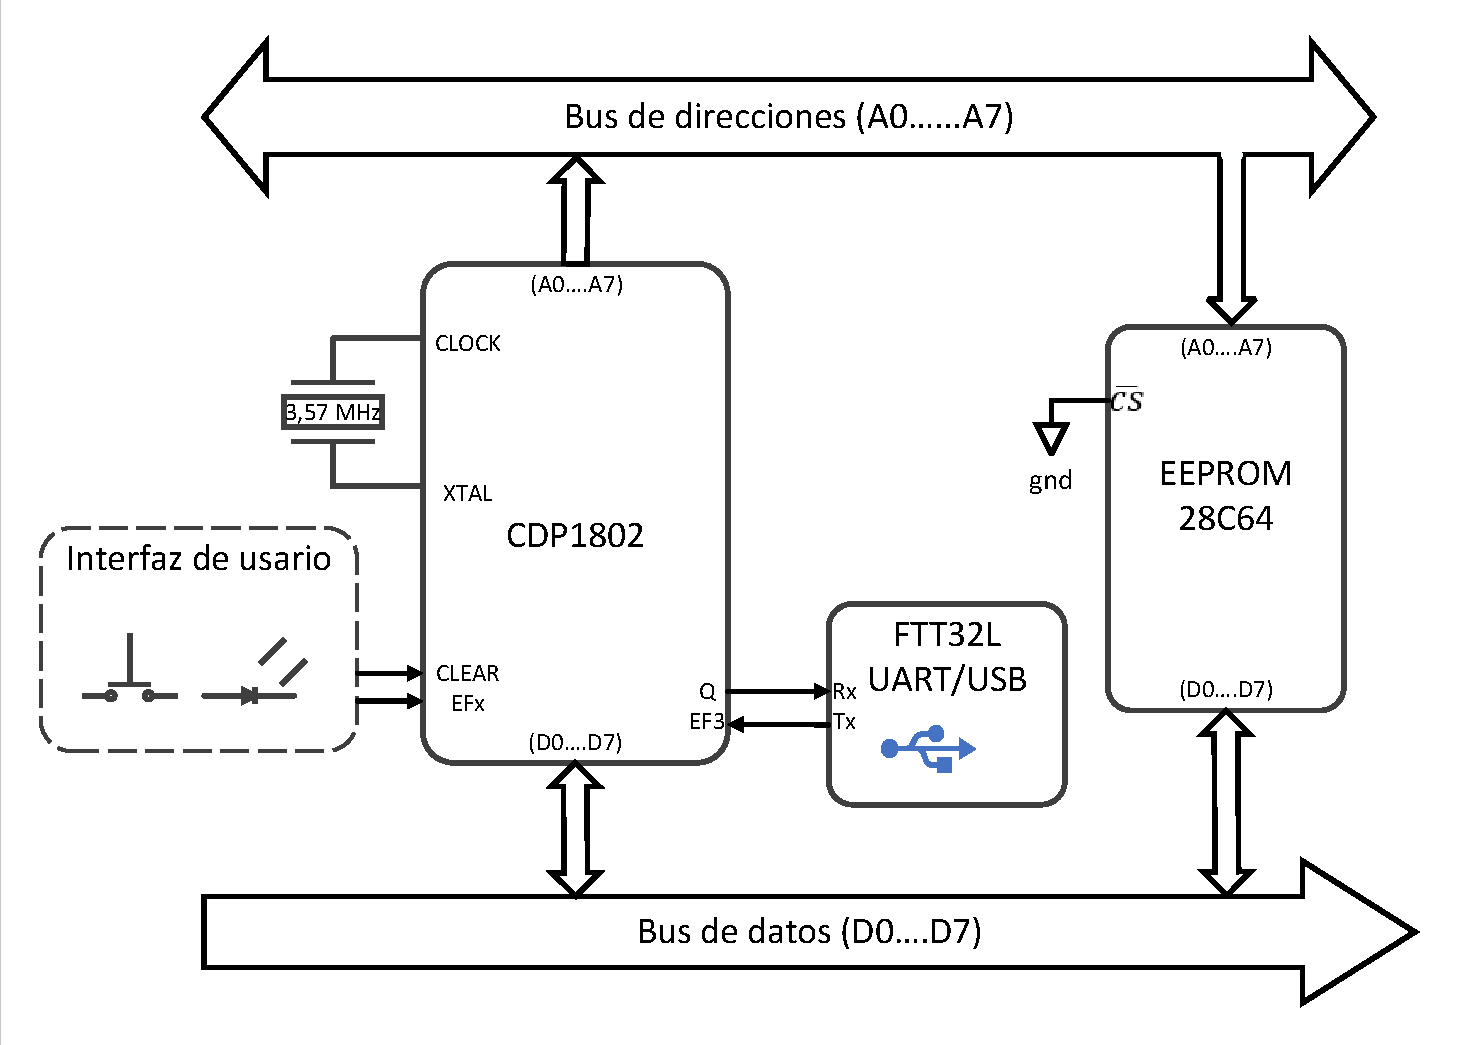
\includegraphics[width=0.9\textwidth]{./imagenes/diag_bloq_sistema_minimo.pdf}
  \caption{Diagrama de bloques del sistema mínimo}
  \label{F:diag_bloq_sistema_minimo}
\end{figure}

El microprocesador es el elemento central del circuito diseñado, que es donde se realiza todo el procesamiento de datos. La incorporación del mismo permite realizar pruebas de funcionamiento, facilitando el entendimiento del lenguaje de programación y la secuencia de las instrucciones y ejecución dentro del microprocesador. Por otro lado, la memoria dentro de este sistema cumple la función de almacenar las instrucciones del programa a ejecutar y no se utiliza la misma para guardar datos generados en ejecución. Debido a la simplicidad del sistema presentado y la arquitectura del microprocesador, solo se utilizó un direccionamiento de 8 bits, lo que limita el tamaño del programa principal a un máximo de 256 bytes. Esto se debe a que el direccionamiento de 16 bits requiere el agregado de más elementos al circuito lo cual se explica en el desarrollo del sistema medio en la sección~\ref{C:SistemaMedio}. Con esta arquitectura los programas desarrollados debían ser simples con el único objetivo de determinar y comprobar el correcto funcionamiento de las conexiones y lograr un entendimiento básico del lenguaje de programación y del microprocesador. Para este fin se utilizan los programas desarrollados y presentados en la sección~\ref{C:ProgramasSMin}.

Debido a las limitaciones en el direccionamiento, se dispuso un diseño que permite establecer el estado de los pines de dirección A8 y A9 de la memoria de programa (28C64), directamente sobre el chip. Esto permite utilizar cuatro sectores de la memoria, aunque no simultáneamente. El microprocesador sigue utilizando únicamente 8 bits para el direccionamiento de memoria. Para la modificación se utilizan puentes tipo jumper que permiten conectar a masa o a VCC tanto A8 como A9 individualmente. De esta forma se establece un mapa de memoria como el presentado en la figura~\ref{F:Mapa_SMin}. De esta manera al realizar el grabado de la memoria EEPROM se pueden incluir los cuatro programas presentados en la sección \ref{C:ProgramasSMin} y pueden ser probados sin necesidad de regrabar la memoria.

\begin{figure}[ht!]
\centering
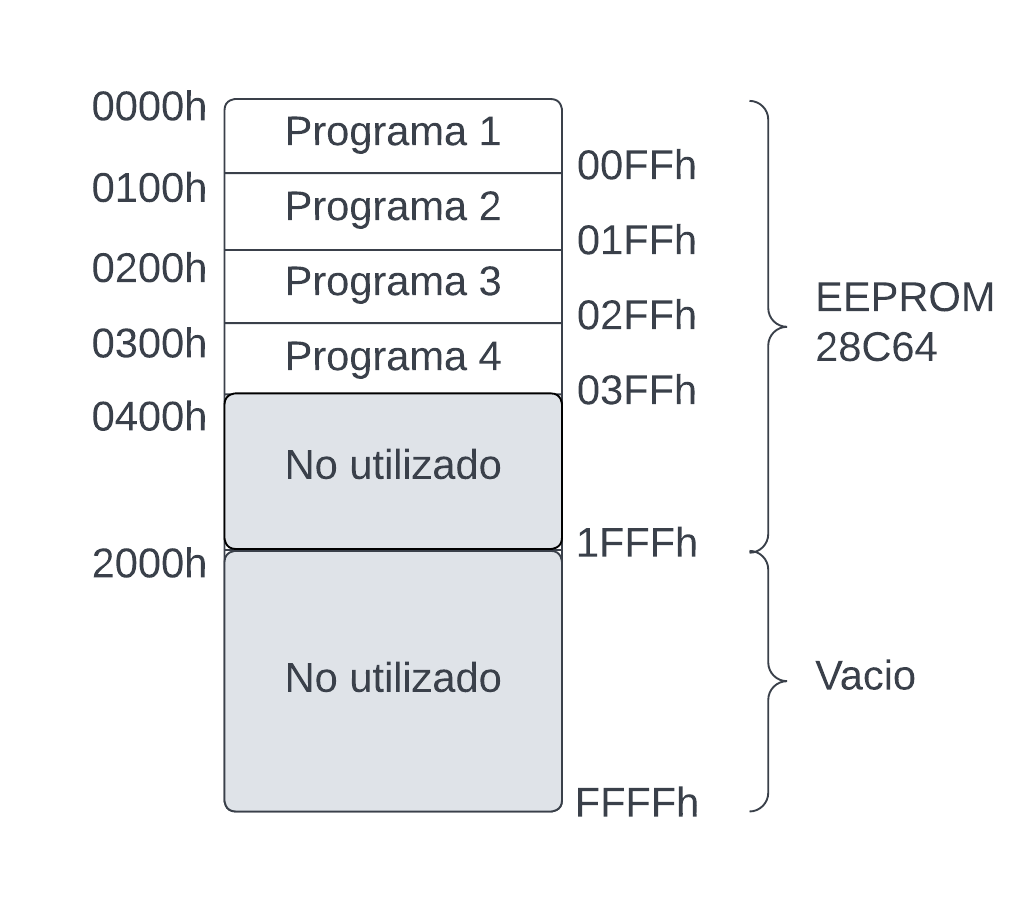
\includegraphics[width=0.57\textwidth]{./imagenes/Mapa_SMin.png}
\caption{\centering Mapa de memoria Sistema Mínimo}
\label{F:Mapa_SMin}
\end{figure}

\clearpage
Para elegir cada uno de los programas debe conectarse adecuadamente un jumper en los conectores de J10 y otro jumper en los conectores de J11, como se describe a continuación.

\begin{description}
    \item[Programa 1:] Conectar un jumper en los pines 2 y 3 de J10, y otro jumper en los pines 2 y 3 de J11.
    \item[Programa 2:] Conectar un jumper en los pines 1 y 2 de J10, y otro jumper en los pines 2 y 3 de J11. 
    \item[Programa 3:] Conectar un jumper en los pines 2 y 3 de J10, y otro jumper en los pines 1 y 2 de J11. 
    \item[Programa 4:] Conectar un jumper en los pines 1 y 2 de J10, y otro jumper en los pines 1 y 2 de J11. 
\end{description}

Para que el circuito funcione correctamente se implementó un sistema de alimentación basado en un regulador de tensión de 5~V, específicamente el UTC7805. La incorporación del mismo proporciona mayor estabilidad en la alimentación protegiendo a los circuitos integrados del sistema. También se incorporó una interfaz de usuario simple que consta de pulsadores como sistema de entrada y LED indicadores de funcionamiento. 

Para la realización del esquemático y el diseño de la placa PCB se utilizó el programa KiCad. El esquema obtenido se presenta en la figura~\ref{F:EsquemaSMin}, además se lo presenta en el apéndice donde se encuentra en tamaño original. La placa PCB diseñada es una simple faz, la pista generada se presenta en la figura~\ref{F:PistaSMin}, mientras que la máscara de componentes de la misma se presenta en la figura~\ref{F:MascaraSMin}.

\begin{figure}[ht]
  \centering
  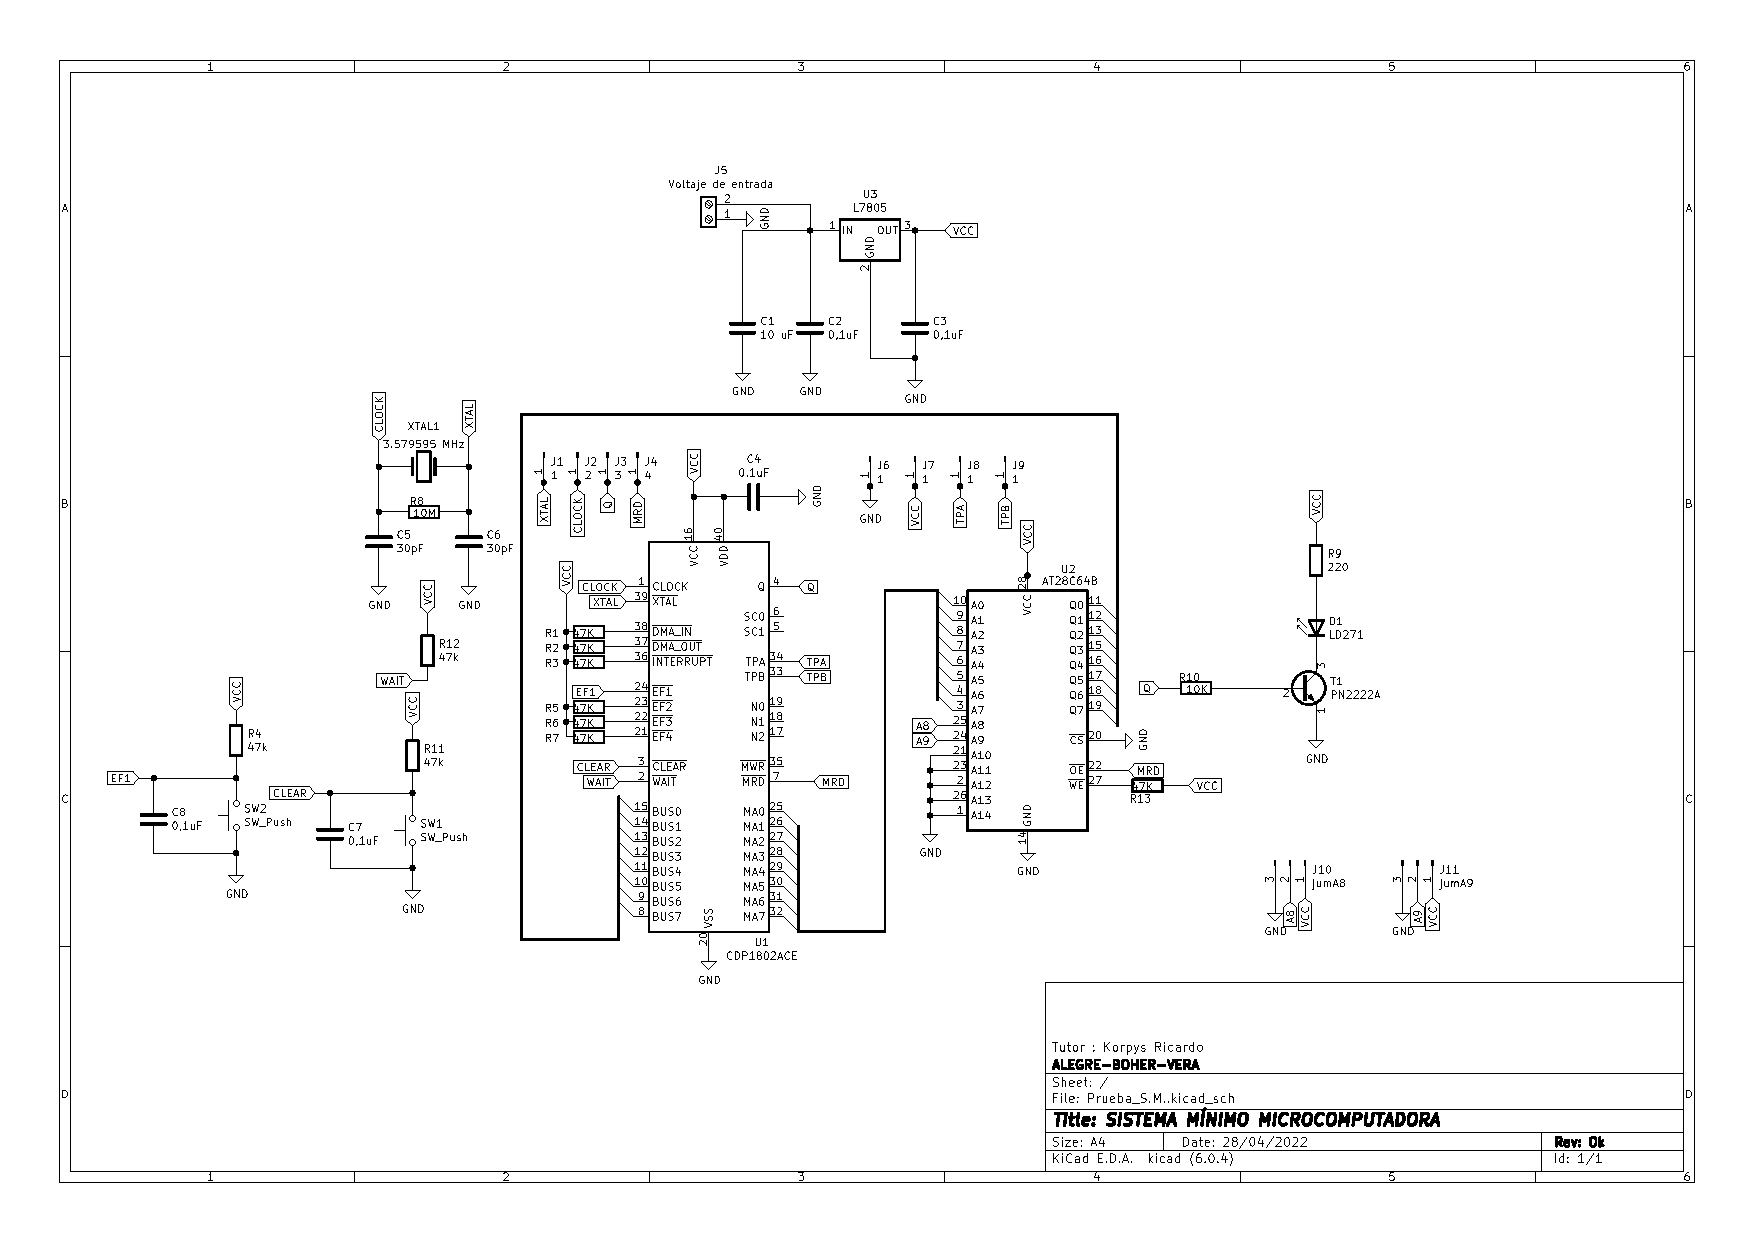
\includegraphics[width=1.2\textwidth, angle=90]{./imagenes/Esq_S.Min..pdf}
  \caption{Esquema de sistema mínimo}
  \label{F:EsquemaSMin}
\end{figure}




\begin{figure}[ht]
\centering
\subfloat[Pista diseñada para sistema mínimo]{
	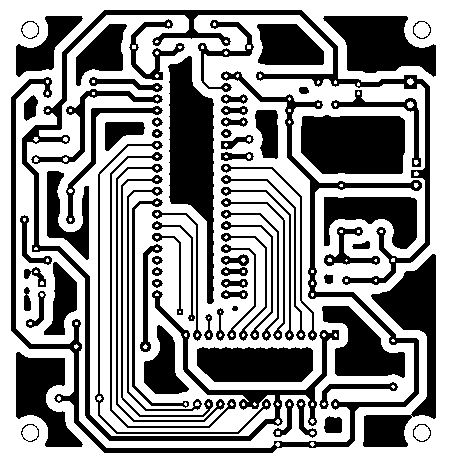
\includegraphics[width=0.52\textwidth]{./imagenes/PistaSMin.png}
	\label{F:PistaSMin}}

\subfloat[Máscara de componentes sistema mínimo]{
	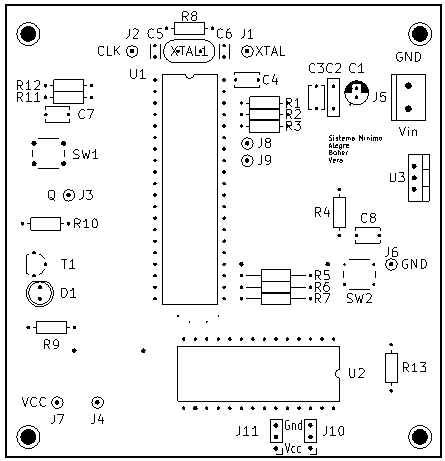
\includegraphics[width=0.51\textwidth]{./imagenes/MascaraSMin.png}
	\label{F:MascaraSMin}}
\caption{Placa PCB diseñada para sistema mínimo}
\label{F:PlacaPCB}
\end{figure}

\clearpage

A partir de los diagramas presentados se procedió a la construcción del circuito. El resultado obtenido se presenta en la fotografía~\ref{F:SMin}. El mismo funcionó correctamente sin necesidad de realizar modificaciones a la arquitectura propuesta. Sin embargo, para la prueba de transmisión de datos mediante UART, con el programa que se presentará en la sección~\ref{C:ComunicacionSerial}, se utilizó una interfaz externa para la conversión del sistema UART a USB, esto permite la recepción de la información en una terminal. La interfaz utilizada es el circuito FT232RL\cite{datasheet_FT232RL}, la cual fue contemplada para los diseños posteriores al sistema mínimo. 

\begin{foto}[ht]
  \centering
  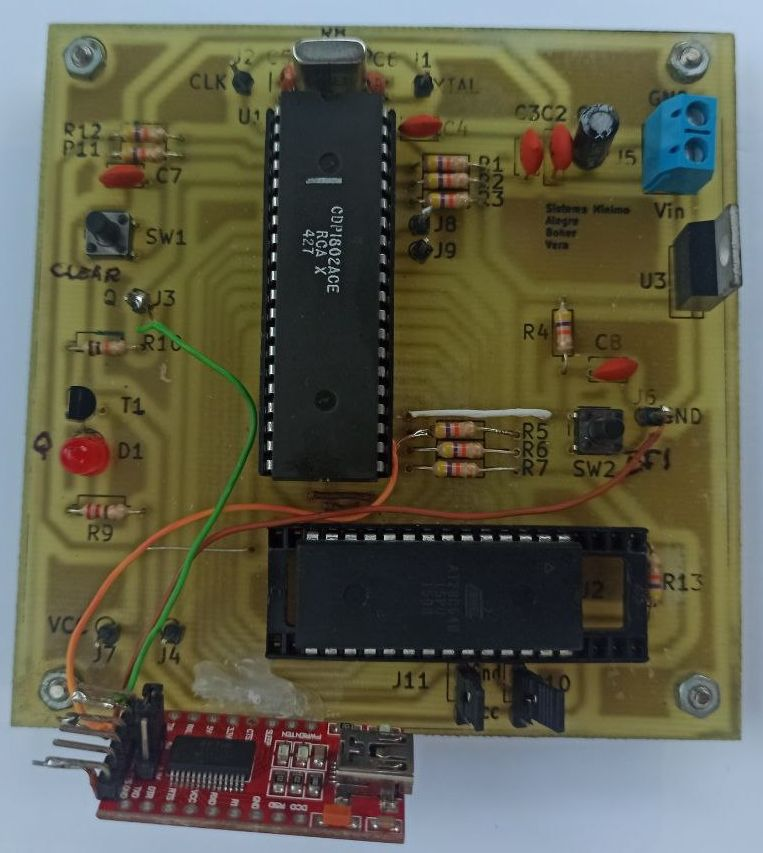
\includegraphics[width=0.5\textwidth]{./imagenes/foto_sistema_min.jpg}
  \caption{Sistema mínimo construido}
  \label{F:SMin}
\end{foto}

\clearpage
\section{Lista de componentes}

En la tabla~\ref{T:bom_sis_min} se encuentra la lista de materiales para la construcción del sistema mínimo.

\begin{table}[ht!]
\caption{Lista de componentes del sistema mínimo}
\label{T:bom_sis_min}
\footnotesize
\begin{tabular}{|p{0.08\textwidth}|p{0.11\textwidth}|p{0.30\textwidth}|p{0.14\textwidth}|p{0.15\textwidth}|}
\hline
Cantidad & Etiqueta \newline
           Identificador            & Descripción                               & Fabricante            & Número de parte \\ \hline \hline
1       & U1                        & Microprocesador                           & RCA                   & CDP1802ACE      \\ \hline
1       & U2                        & Memoria EEPROM 8k x 8                     & ATMEL                 & AT28C64B          \\ \hline
1       & U3                        & Regulador de tensión                      & YOUW ANG              & UTC7805          \\ \hline
1       & T1                        & Transistor BJT NPN                        & ST Microelectronics   & PN2222A           \\ \hline
1       & XTAL1                     & Cristal \num{3.579545}~\si{\mega\hertz}   & CQ Electronics        & \listaVacio                \\ \hline
2       & SW1, SW2                  & Pulsador 6mm~x~4,3mm                      & \listaVacio           & \listaVacio       \\ \hline
10      & R1, R2, R3, R4, R5, R6, R7, R11, R12, R13
                                    & Resistor 47~\si{\kilo\ohm} 1/8~\si{\watt} & \listaVacio                      & \listaVacio                \\ \hline
1       & R8                        & Resistor 10~\si{\mega\ohm} 1/8~\si{\watt} & \listaVacio                      &    \listaVacio             \\ \hline
1       & R9                        & Resistor 220~\si{\ohm} 1/4~\si{\watt}     & \listaVacio                      &    \listaVacio             \\ \hline
1       & R10                       & Resistor 10~\si{\kilo\ohm} 1/8~\si{\watt} &  \listaVacio                     &  \listaVacio               \\ \hline
1       & D1                        & LED Rojo 5mm                              & \listaVacio                      &  \listaVacio               \\ \hline
1       & C1                        & Capacitor electrolítico 10~\si{\micro\farad} 25~\si{\volt}
                                                                                &  \listaVacio                     &   \listaVacio              \\ \hline
5       & C2, C3, C4, C7, C8        & Capacitor cerámico \num{0.10}~\si{\micro\farad} 50~\si{\volt}
                                                                                &  \listaVacio                     & \listaVacio                \\ \hline
2       & C5, C6                    & Capacitor cerámico \num{30}~\si{\pico\farad} 50~\si{\volt}
                                                                                & \listaVacio                      & \listaVacio                \\ \hline
8       & J1, J2, J3, J4, J6, J7, J8, J9
                                    & Pin conector macho (1 \textit{Male Header Pin})
                                                                                & \listaVacio                      &  \listaVacio               \\ \hline
1       & J5                        & Bornera 2 pines \num{5.08}~mm             & \listaVacio                      &  \listaVacio               \\ \hline
2       & J10, J11                  & 1x3 Pines Conectores Macho \num{2.54}~mm        & \listaVacio                      & \listaVacio                \\ \hline
\end{tabular}
\normalsize
\end{table}

Algo no contemplado en esta lista de componentes es el módulo FT232RL~\cite{datasheet_FT232RL}, dado que fue soldado luego de armado el circuito, como puede apreciarse en la figura~\ref{F:SMin}. El módulo FT232RL tiene soldado con cables sus pines Rx, Tx, Vcc y GND, a los pines Q, EF2, Vcc y GND del microprocesador, respectivamente.

%%-------------------------------------------------------------------------------------------

\clearpage
\section{Programas del sistema mínimo}
\label{C:ProgramasSMin}
Para probar el sistema mínimo, se confeccionaron cuatro programas sencillos de no más de 256 bytes, debido a que el sistema mínimo no puede direccionar más que esta cantidad de direcciones de memoria. Los programas se presentan a continuación, haciendo uso de diagramas de flujo. Sin embargo, en el apéndice~\ref{C:anexo-programas-sistema-mínimo} se encuentra el código fuente de los cuatro programas.

\subsection{Programa 1: Parpadeo LED Q}

El primer programa hace parpadear el LED conectado a la salida Q del microprocesador. Para ello, como puede apreciarse en el diagrama de flujo de la figura~\ref{F:prog_1}, el programa comienza apagando el LED (Q~=~0), luego realiza un retardo por software, que consiste en la asignación de un valor específico a un registro, para luego decrementarlo hasta que llegue a cero. Una vez finalizado el retardo, el LED togglea; si está encendido, se apaga, y si está apagado, se enciende. Esta secuencia se repite constantemente, haciendo parpadear el LED conectado a la salida Q. En el apéndice~\ref{C:anexo-prog-1}, se encuentra el código fuente del programa~1.

\begin{figure}[ht]
  \centering
  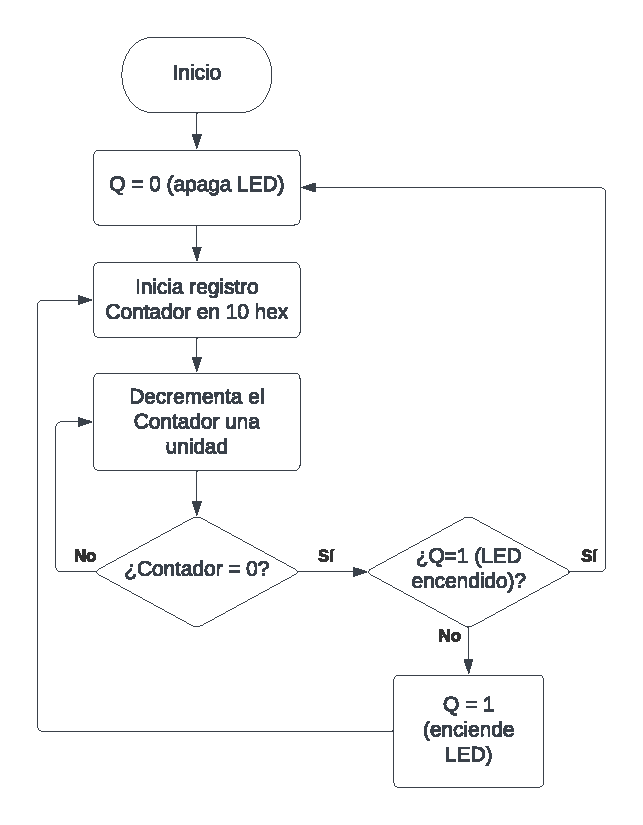
\includegraphics[width=0.5\textwidth]{./imagenes/programa_1.pdf}
  \caption{Programa 1}
  \label{F:prog_1}
\end{figure}

\clearpage
\subsection{Programa 2: LED Q se enciende al presionar pulsador}

El programa dos permite al usuario interactuar con el sistema, de manera que se prueba el funcionamiento de las entradas EFx (en el caso del sistema mínimo, EF1, dado que allí se encuentra conectado el pulsador). En el diagrama de flujo de la figura~\ref{F:prog_2} se puede observar cómo opera el programa. Cuando el botón se encuentra presionado, el programa entra a un bucle infinito que ejecuta el comando para encender el LED, en caso contrario, el programa entra a un bucle similar, pero donde la instrucción que se ejecuta continuamente es la de apagado del LED. En el apéndice~\ref{C:anexo-prog-2}, se encuentra el código fuente del programa~2.

\begin{figure}[H]
  \centering
  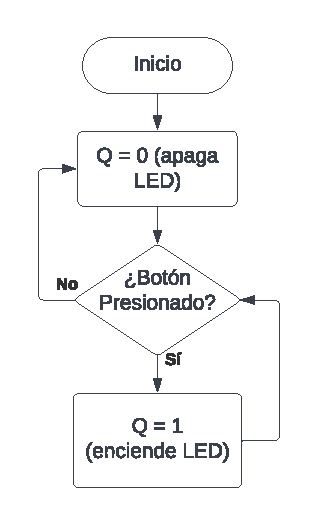
\includegraphics[width=0.3\textwidth]{./imagenes/programa_2.pdf}
  \caption{Programa 2}
  \label{F:prog_2}
\end{figure}

\clearpage
\subsection{Programa 3: LED Q parpadea al presionar pulsador}

El programa 3 es una combinación de los dos programas previos, el mismo hace parpadear el LED conectado a la salida Q del microprocesador, pero lo hace solo si el usuario presiona el pulsador.

En la figura~\ref{F:prog_3} se encuentra el diagrama de flujo del programa, el mismo consiste de una rutina de retardo con un contador que disminuye hasta cero (como en el programa 1), y luego, si el pulsador se encuentra presionado, el LED comienza a parpadear, pero si el pulsador no se encuentra presionado, el LED permanece apagado. En el apéndice~\ref{C:anexo-prog-3}, se encuentra el código fuente del programa 3.

\begin{figure}[H]
  \centering
  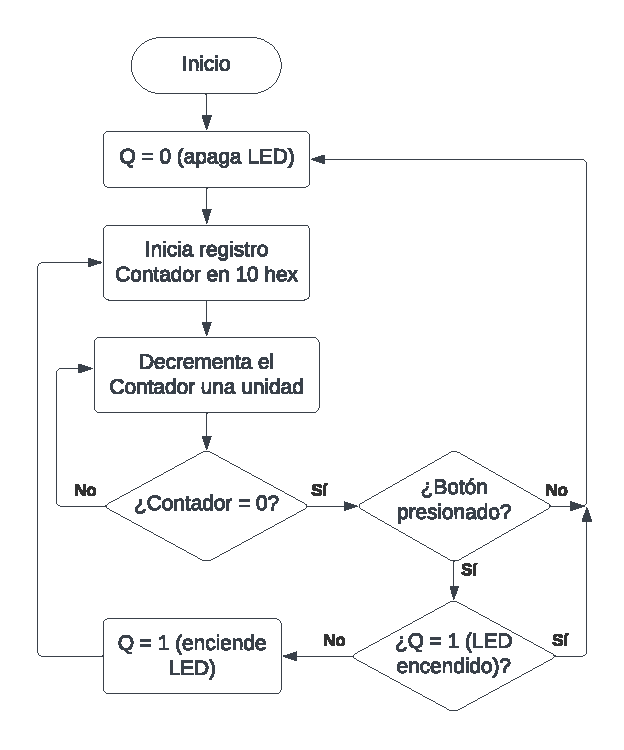
\includegraphics[width=0.6\textwidth]{./imagenes/programa_3.pdf}
  \caption{Programa 3}
  \label{F:prog_3}
\end{figure}

\clearpage
\subsection{Programa 4: Transmisión serial de caracteres}
\label{C:ComunicacionSerial}

El programa 4 realiza la transmisión serial por protocolo UART a través del pin Q de los caracteres “ABCDEFG”, seguido de un retorno de carro y un salto de línea. Este es el más complejo de los programas confeccionados para el sistema mínimo, por lo tanto, se encuentra descripto en dos diagramas de flujo separados, uno para la rutina principal, figura~\ref{F:prog_4_main} y otro para la rutina de transmisión de datos, figura~\ref{F:prog_4_rut_trans}. Si es de interés para el lector, en el apéndice~\ref{C:anexo-prog-4} se encuentra el código fuente.

 En la rutina principal, figura~\ref{F:prog_4_main}, inicialmente se inicializa el registro Contador  (en 7 decimal), que se utiliza para realizar la misma rutina 7 veces, y el registro Carácter (en 65 decimal), el cual representa el carácter A del código ASCII. Luego se ejecuta un bucle 7 veces seguidas, utilizando para ello el registro Contador. El mismo se decrementa una unidad en cada repetición del bucle y al llegar a cero en la última repetición, el programa sigue con su rutina. Dentro del bucle, Carácter es asignado a otro registro denominado Dato\footnote{Esta asignación parece a primera vista redundante, pero la razón de ello es que la rutina de trasmisión modifica el registro Dato, por lo tanto, se requiere que el dato a trasmitir permanezca guardado en otro lado, en este caso en el registro Carácter.}, en este registro debe encontrarse el dato a ser transmitido por la rutina de transmisión, seguidamente se llama a esa rutina, enviando el primer carácter (letra A). Seguidamente se llama a una rutina de retardo, se incrementa Carácter (pasando al siguiente carácter ASCII) y se vuelve a transmitir. Luego de ejecutarse 7 veces este bucle, se han transmitido los caracteres “ABCDEFG”.

A continuación, se sale del bucle y se envían los caracteres retorno de carro (D hexadecimal en codificación ASCII) y salto de línea (A hexadecimal en codificación ASCII). Esto concluye la rutina principal, la cual, al finalizar, vuelve a ejecutarse desde el comienzo.

En cuanto a la rutina de transmisión, figura~\ref{F:prog_4_rut_trans}, la misma envía los datos de forma serial por protocolo UART utilizando para ello el pin Q del microprocesador como salida de transmisión. En el apéndice~\ref{C:anexo-comunicación-serial} (\nameref{C:anexo-comunicación-serial}) se encuentran explicados los detalles relacionados con este protocolo.

La rutina de transmisión comienza pasando el pin Q de su estado de reposo (Q~=~1) a estado bajo (Q~=~0) por un periodo de 1~bit-time, este es el bit de inicio de la trama UART. Luego se inicializa un contador en 8 decimal, para realizar un bucle que se repite 8 veces, una por cada bit del dato de 8 bits. En este bucle el dato a enviar se corre a la derecha, cargando el LSB en el bit DF interno del microprocesador, en base al valor de este bit, se decide si poner la línea en estado alto (Q~=~1) o bajo (Q~=~0). Esto se repite 8 veces, de manera tal que se envían todos los bits del dato, del LSB al MSB. Finalmente se envían dos bits de parada (Q~=~1) para terminar la transmisión del dato.

\begin{figure}[H]
\centering
\subfloat[Rutina principal]{
	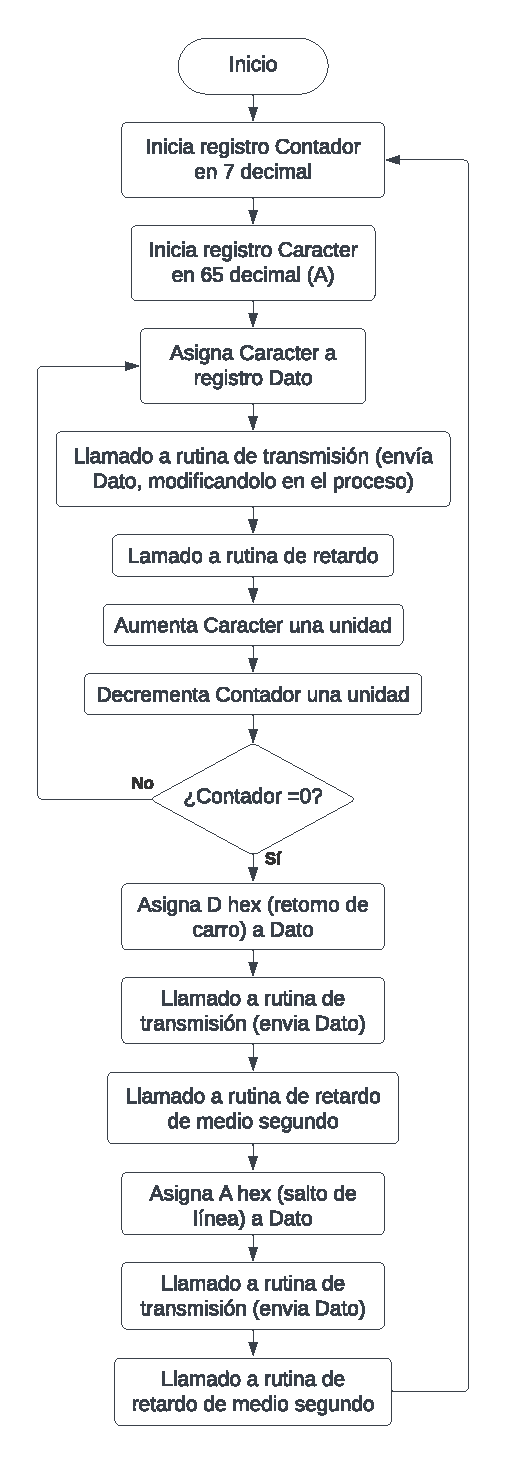
\includegraphics[width=0.45\textwidth]{./imagenes/programa_4_main.pdf}
	\label{F:prog_4_main}}
\quad
\subfloat[Rutina de transmisión]{
	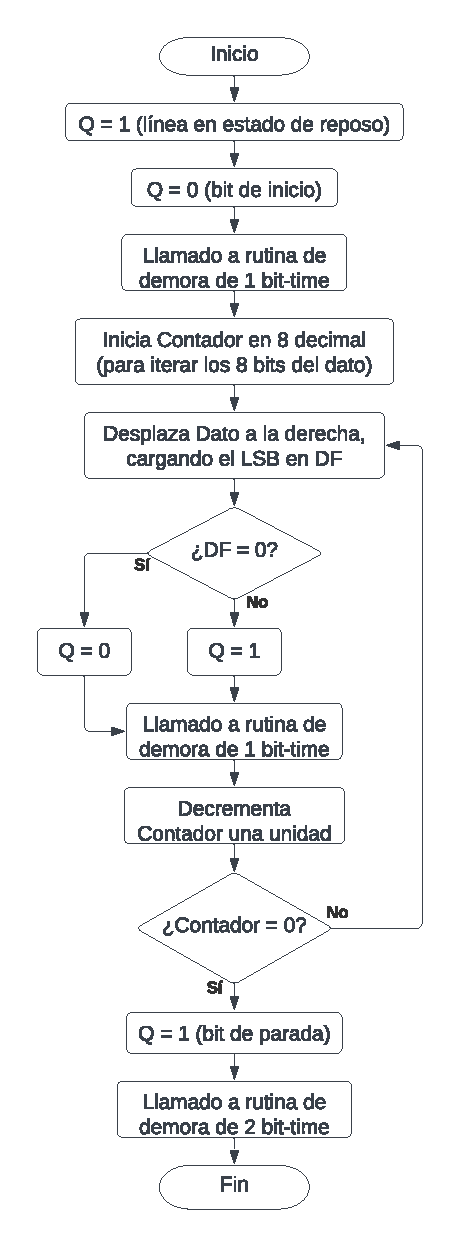
\includegraphics[width=0.45\textwidth]{./imagenes/program_4_rut_de_trans.pdf}
	\label{F:prog_4_rut_trans}}
\caption{Programa 4}
\label{F:prog_4}
\end{figure}

El programa 4 cuenta con muchas subrutinas, todas ellas fueron escritas con el método denominado \entreComillas{SEP technique}, el cual se encuentra descrito, junto a otros métodos, en la página 130 del libro Design Ideas Book for the CDP1802 COSMAC Microprocessor\cite{cdp1802_design_ideas}. El método SEP para las subrutinas fue utilizado por no requerir RAM para su operación, algo necesario, dado que el sistema mínimo no posee RAM.

En el listado~\ref{L:retardo}, se encuentra la rutina de retardo de un bit-time. En cada línea, como comentario, está indicado, para cada instrucción, el número de bytes, el número de ciclos máquina y la cantidad de veces que se ejecuta cada instrucción al llamarse la rutina. Esta información nos permite determinar el retardo ocasionado por la misma, necesario para poder calcular el valor que debe cargarse en \texttt{R1} (línea 5 y 6) y así poder obtener el retardo necesario.

\footnotesize
\lstinputlisting[language=CDP1802, caption = {Rutina de retardo de 1 bit-time}, label = {L:retardo}]{codigo/delay_routine.asm}
\normalsize

En base a esta información, en \eqref{eq:retardo} se tiene la expresión para el retardo; teniendo en cuenta que: todas las instrucciones ejecutadas en la rutina tienen una duración de dos ciclos máquina y que un ciclo máquina equivale a ocho ciclos de reloj.

\begin{equation}
    Retardo = 2\:ciclosMaq\:(4+3\:CONT1BT)\frac{8\:ciclosReloj}{1\:cicloMaq} T_{reloj}
    \label{eq:retardo}
\end{equation}

Simplificando \eqref{eq:retardo}, se obtiene \eqref{eq:retardo_simplificado}.

\begin{equation}
    Retardo = 16\:(4+3\:CONT1BT) T_{reloj}
    \label{eq:retardo_simplificado}
\end{equation}

Finalmente, a partir de \eqref{eq:retardo_simplificado}, se despeja CONT1BT, obteniéndose \eqref{eq:contador}.

\begin{equation}
    CONT1BT = \frac{Retardo}{48\:T_{reloj}}-\frac{4}{3}
    \label{eq:contador}
\end{equation}

En base a \eqref{eq:contador}, y teniendo en cuenta que el sistema mínimo utiliza un cristal de \num{3.579545}~\si{\mega\hertz} ($ T_{reloj} = \left(\num{3.579545}~\si{\mega\hertz}\right)^{-1} = \num{279.3651}~\si{\nano\second} $), podemos calcular CONT1BT. Lo único faltante es la duración del retardo, el cual se obtiene simplemente haciendo la inversa del baud rate. Tomando un baudrate de 600~baudios, se obtiene un retardo de \num{0.001666667}~\si{\second}. Con estos datos, y la ecuación \eqref{eq:contador}, es posible calcular el valor del contador para la rutina de retardo de 1 bit-time, como se muestra en \eqref{eq:calculo-1-bit-time-sistema-min}; redondeando el resultado, debido a que se trata de un valor que debe cargarse a un registro de 8 bits.

\begin{equation}
    CONT1BT = \frac{Retardo}{48\:T_{reloj}}-\frac{4}{3} = \frac{\num{0.001666667}~\si{\second}}{48\cdot\num{279.3651}~\si{\nano\second}}-\frac{4}{3} = \num{122.96}\approx\num{123}
    \label{eq:calculo-1-bit-time-sistema-min}
\end{equation}

\section{Simulaciones y resultados experimentales}

Todos los programas fueron probados en el simulador Emma02 antes de ser implementados en el sistema mínimo, los resultados obtenidos fueron los deseados. Para el testeo se utilizó la computadora Membership Card, y la configuración exacta utilizada puede visualizarse en la figura~\ref{F:config_emma02_sis_min}.

\begin{figure}[ht!]
  \centering
  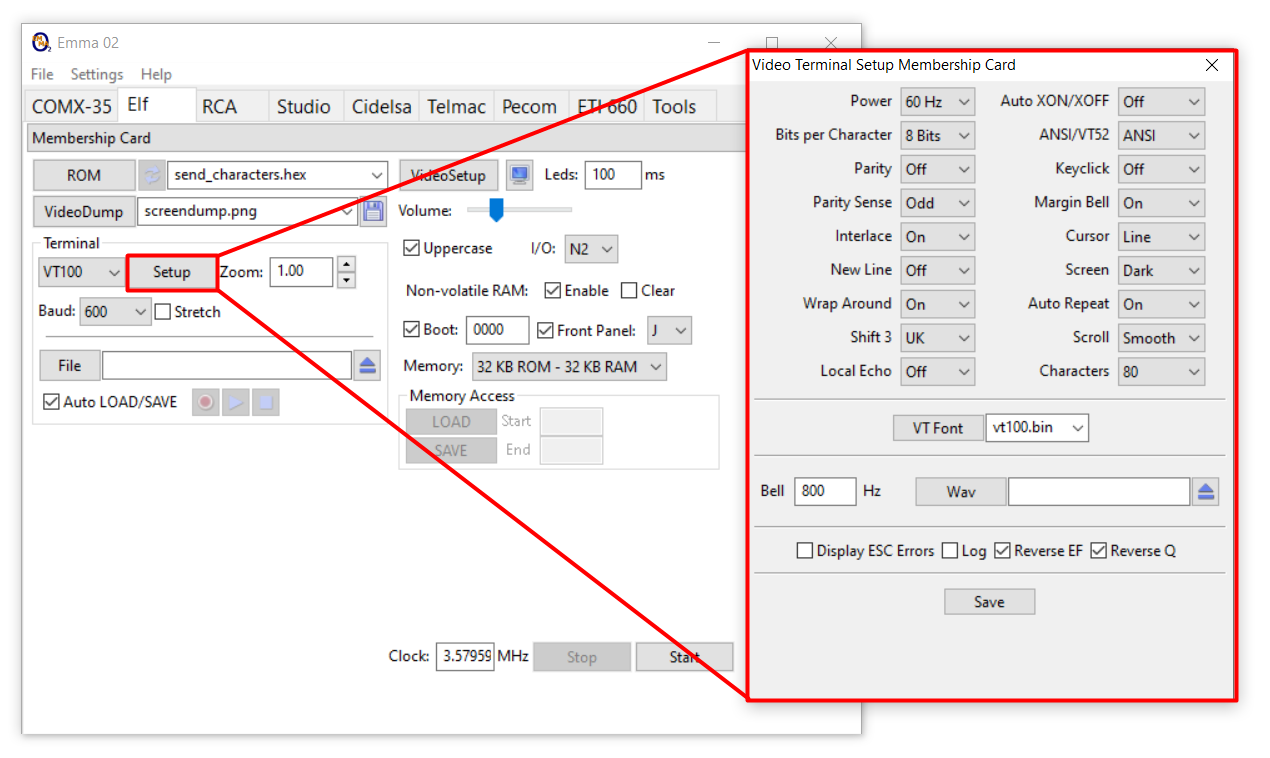
\includegraphics[width=1\textwidth]{./imagenes/config_emma02_sis_min.png}
  \caption{Configuración utilizada en el simulador Emma02}
  \label{F:config_emma02_sis_min}
\end{figure}

En la figura~\ref{F:prog_4_resultados} puede observarse el resultado obtenido tanto en simulación como en el sistema mínimo construido. Los resultados obtenidos en ambos casos fueron acordes a lo esperado. La configuración en Tera Term fue de 600~baudios, 8~bits para tamaño de datos, sin bit de paridad y con dos bits de parada.

\begin{figure}[H]
\centering
\subfloat[Resultado obtenido en Emma02]{
	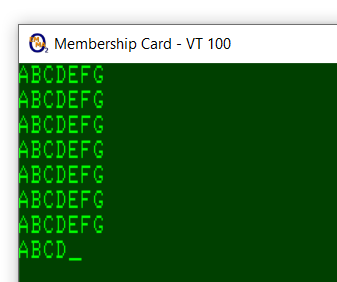
\includegraphics[width=0.45\textwidth]{./imagenes/programa_4_emma02.png}
	\label{F:programa_4_emma02}}
\quad
\subfloat[\centering Resultado experimental obtenido con el sistema mínimo]{
	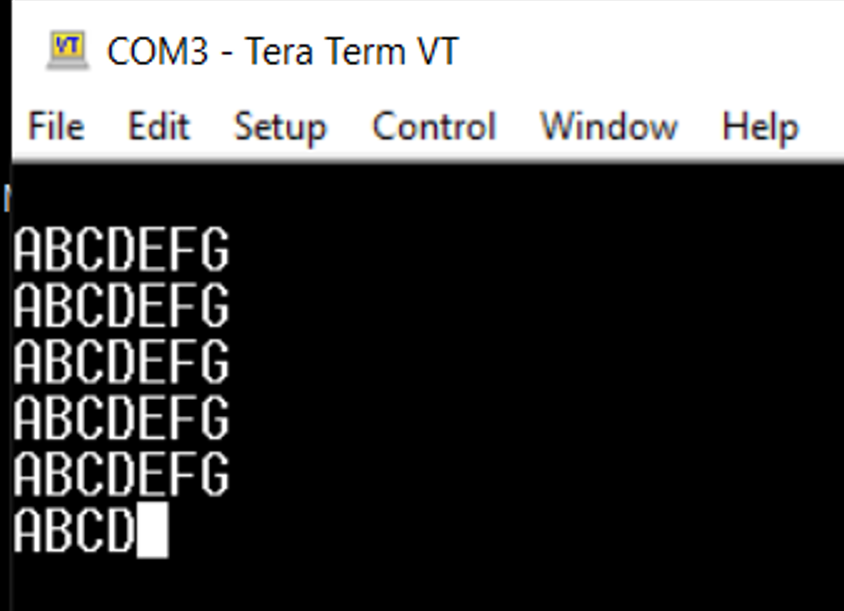
\includegraphics[width=0.45\textwidth]{./imagenes/programa_4_real.png}
	\label{F:programa_4_real}}
\caption{Resultados de la ejecución del programa 4}
\label{F:prog_4_resultados}
\end{figure}

%% agregar captura de los caracteres obtenidos en esta parte, simulación y real juntos
%% explicar que el terminal externo es una computadora aparte corriendo Tera Term

\section{Programador}
Para insertar los programas diseñados en la memoria EEPROM fue requerido el diseño de un circuito programador. El diseño adoptado se basa en un Arduino Nano. El software utilizado para el mismo no es de nuestra autoría, se encuentra disponible en la red \cite{pagina_programador}; aun así, se tuvieron que realizar modificaciones, con ayuda de programación en Python, para obtener un resultado satisfactorio, ya que luego de compilar un programa se disponía del mismo en formato Intel y este debía ser interpretado antes de pasarlo al Arduino que se encargaría de grabar la memoria.



Finalmente, el resultado obtenido con el programador sirvió para realizar unos ensayos y grabar memoria, sin embargo, debido a su dificultad de operación se terminó descartando y se reemplazó por el uso del programador presentado en la sección~\ref{C:Programador}. Aun así, por haberse construido, se presenta el esquemático del circuito en la figura~\ref{F:EsquemaProg} y una fotografía del resultado obtenido en la figura~\ref{F:PlacaProg}.

\begin{figure}[ht]
  \centering
  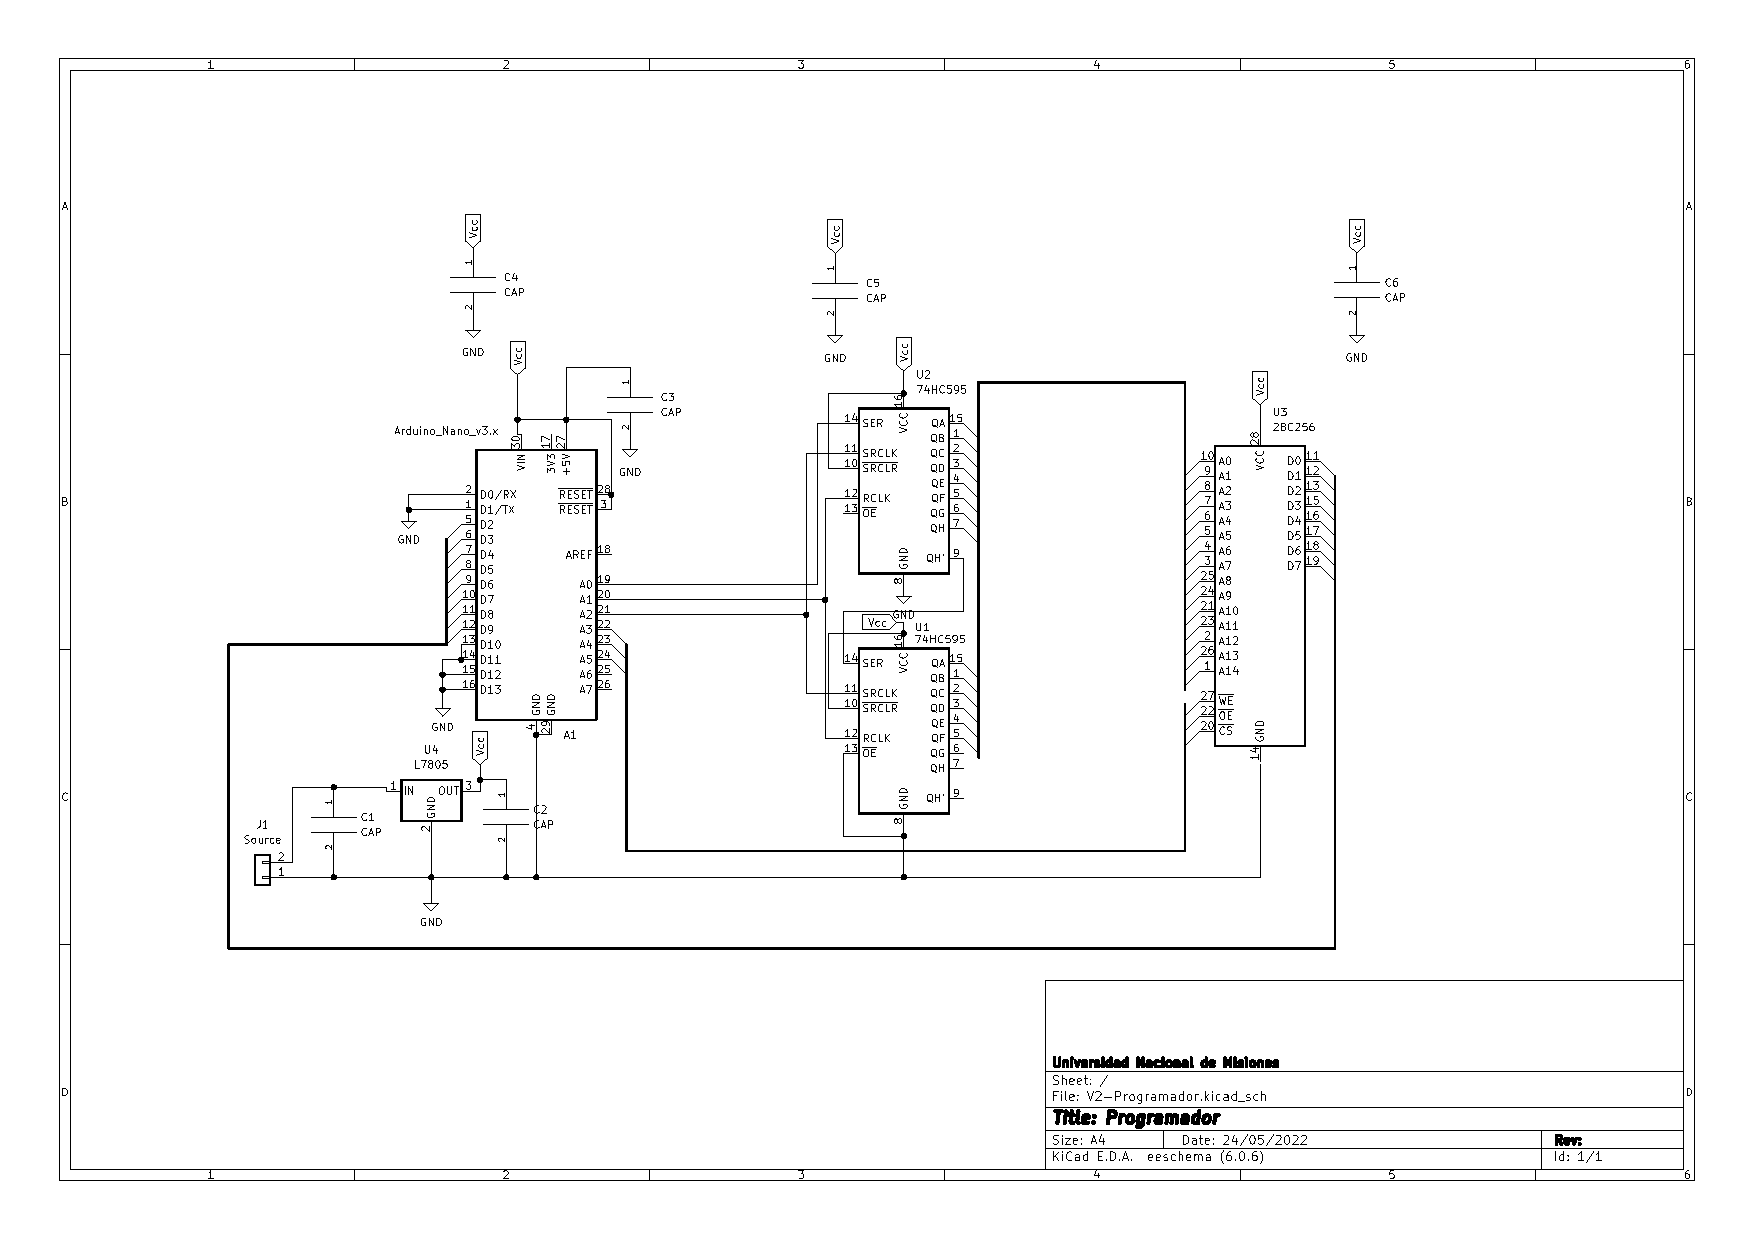
\includegraphics[width=1.2\textwidth, angle=90]{./imagenes/EsqProg.pdf}
  \caption{Esquema de programador}
  \label{F:EsquemaProg}
\end{figure}


\begin{figure}[ht]
\centering
\subfloat[Pista diseñada para Programador]{
	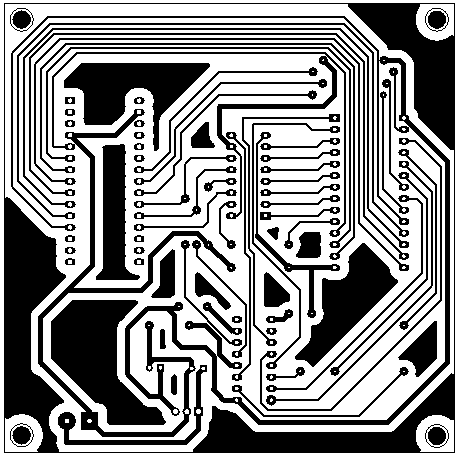
\includegraphics[width=0.52\textwidth]{./imagenes/PistaProg.png}
	\label{F:PistaProg}}

\subfloat[Máscara de componentes de Programador]{
	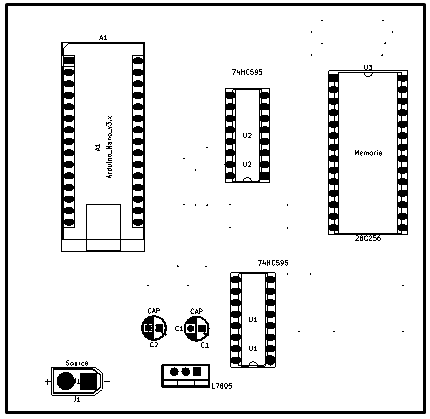
\includegraphics[width=0.51\textwidth]{./imagenes/MascProg.png}
	\label{F:MascaraProg}}
\caption{Placa PCB diseñada para el programador de memoria}
\label{F:PlacaProg}
\end{figure}


\chapter{Sistema medio}
\label{C:SistemaMedio}


El sistema medio se realizó con el objetivo de implementar una arquitectura más compleja que el sistema mínimo, permitiendo desarrollar programas del tipo dinámico en el sistema. Principalmente, se buscaba implementar programas que interactuaban con la memoria del sistema de forma dinámica, es decir, que utilizaban una memoria del tipo RAM, la cual se utiliza en la arquitectura del sistema medio. La diferencia principal con respecto al sistema mínimo es el uso de toda la memoria disponible en el mapa de memoria, permitiendo implementar códigos que requieren de mayor disponibilidad de memoria y por ende son más complejos. 

El microprocesador CDP1802 cuenta con un direccionamiento de 16 bits, no obstante, el mismo utiliza solamente 8 líneas para el bus de direcciones. La solución presentada por el microprocesador para el direccionamiento es enviar primero los 8 bits más significativos de la dirección, luego los 8 bits menos significativos. Para evitar la pérdida de los 8 primeros bits se debe integrar un latch (74HC373) que almacene los primeros 8 bits del bus de direcciones, y el mismo microprocesador sincroniza al latch con una señal para el registro de los datos. 

Es de esta manera que el sistema medio puede direccionar una mayor cantidad de memoria que en el sistema mínimo (256 x 8), utilizando un latch de 8 bits 74HC373\cite{datasheet_74HC373} y aprovechando el mecanismo propuesto por el CDP1802 para aumentar la cantidad de líneas de dirección hasta 16 bits, logrando direccionar 64k x 8. Esto se observa en el diagrama de bloques de la Figura~\ref{F:diag_bloq_sistema_medio}.

 \begin{figure}[H]
  \centering
  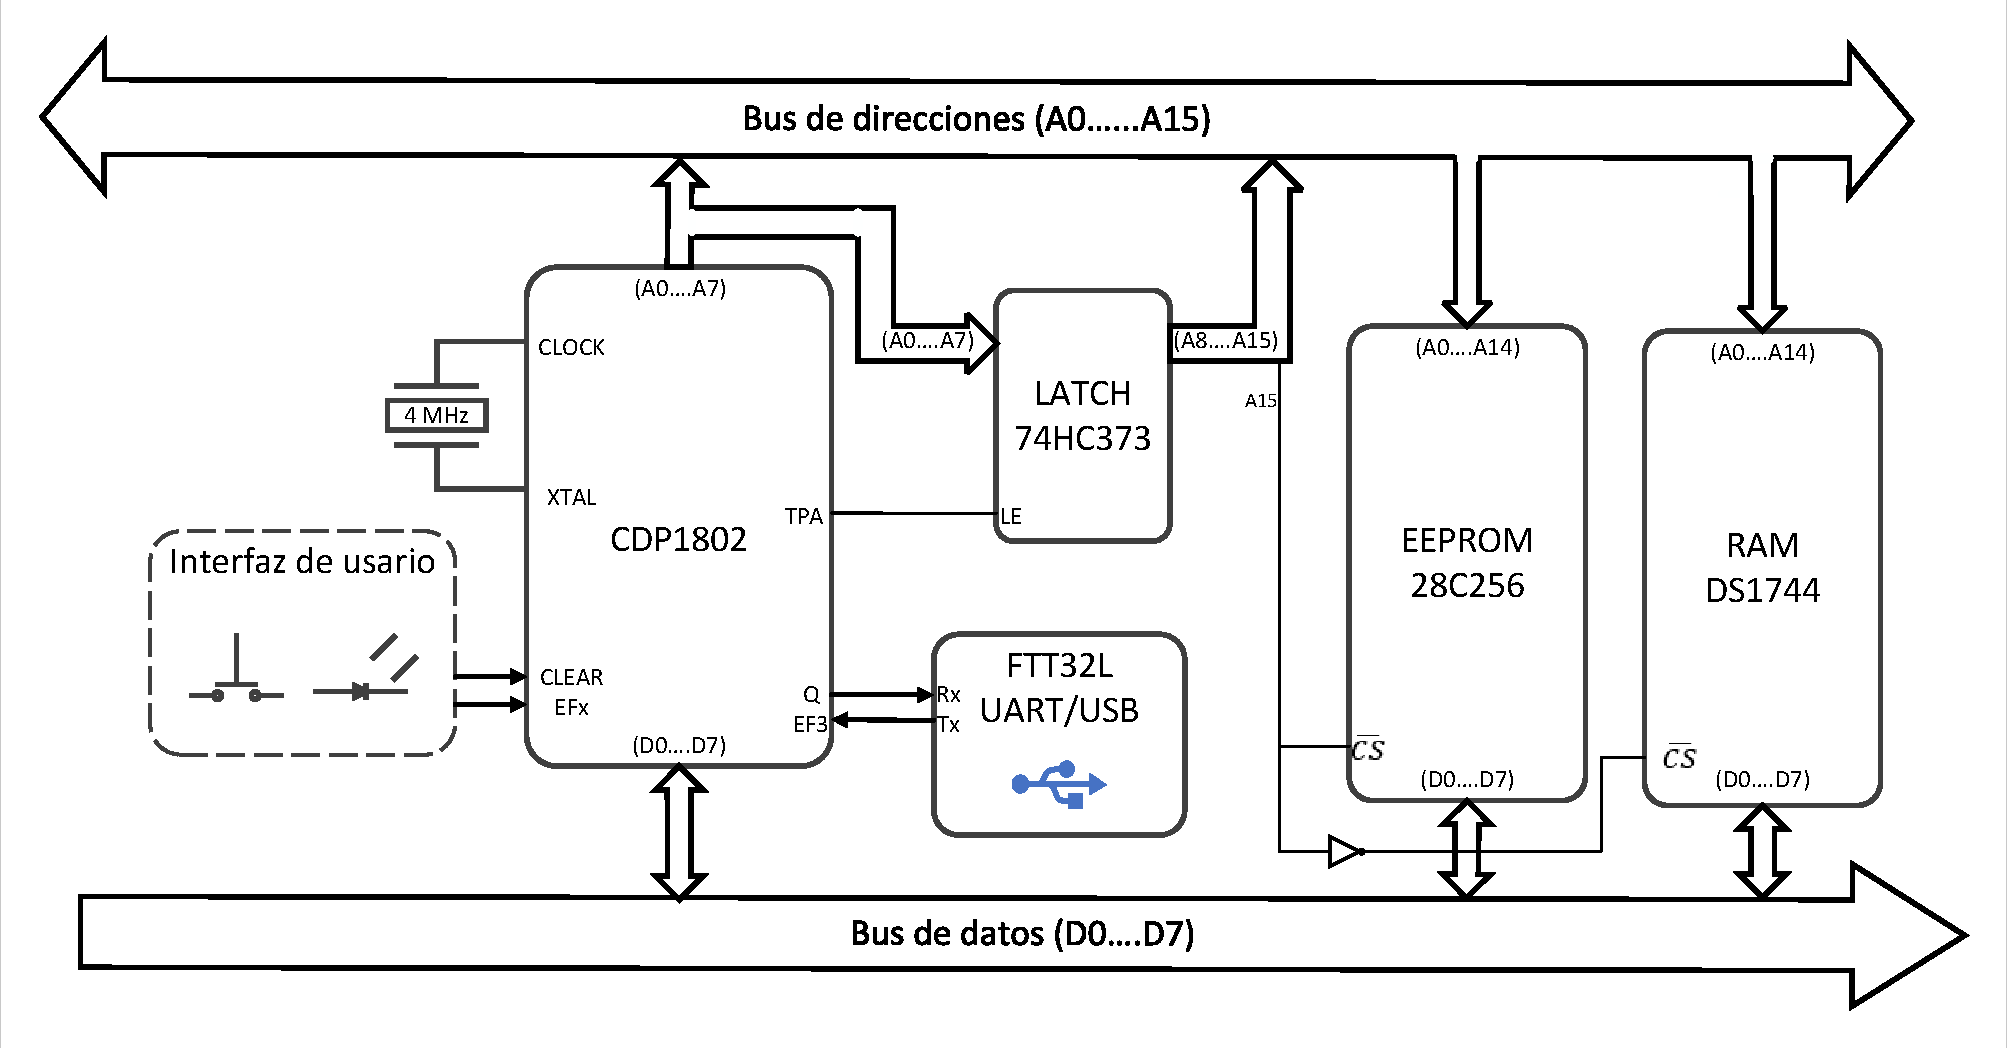
\includegraphics[width=0.98\textwidth]{./imagenes/diag_bloq_sistema_medio.pdf}
  \caption{Diagrama de bloques del sistema medio}
  \label{F:diag_bloq_sistema_medio}
\end{figure}

Esta incorporación de la memoria RAM es la principal diferencia con el sistema mínimo, lo cual se muestra en el mapa de memoria de la Figura~\ref{F:mapa_de_mem_sis_med}, donde se tiene una memoria de programa EEPROM (32k x 8) y una memoria de datos RAM (32k x 8); que en total utilizan toda la capacidad de direccionamiento (64k x 8).

\begin{figure}[ht]
  \centering
  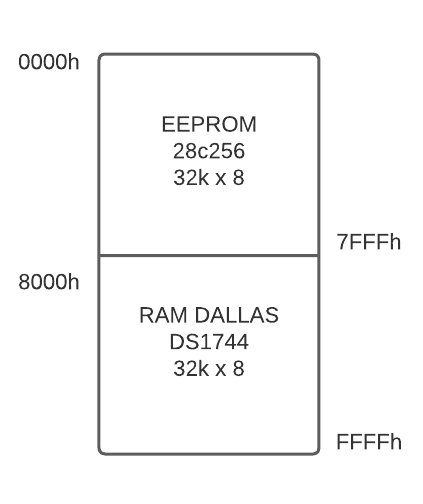
\includegraphics[width=0.4\textwidth]{./imagenes/mapa_de_mem_sis_med.png}
  \caption{Mapa de memoria del sistema medio}
  \label{F:mapa_de_mem_sis_med}
\end{figure}


 
Para realizar la interacción con la terminal externa, se incluyó en el esquema del sistema medio un conversor de UART/USB que dota al sistema de la capacidad de interactuar con una computadora externa, lo cual se explicará mejor en la sección de programas. Los demás dispositivos utilizados son los mismos que en el sistema mínimo y son los requeridos para asegurar el funcionamiento del sistema de forma integral. El esquemático del sistema medio se encuentra en la Figura~\ref{F:esquematico_SME}, el cual fue realizado con el software KiCad. 

 \begin{figure}[ht]
  \centering
  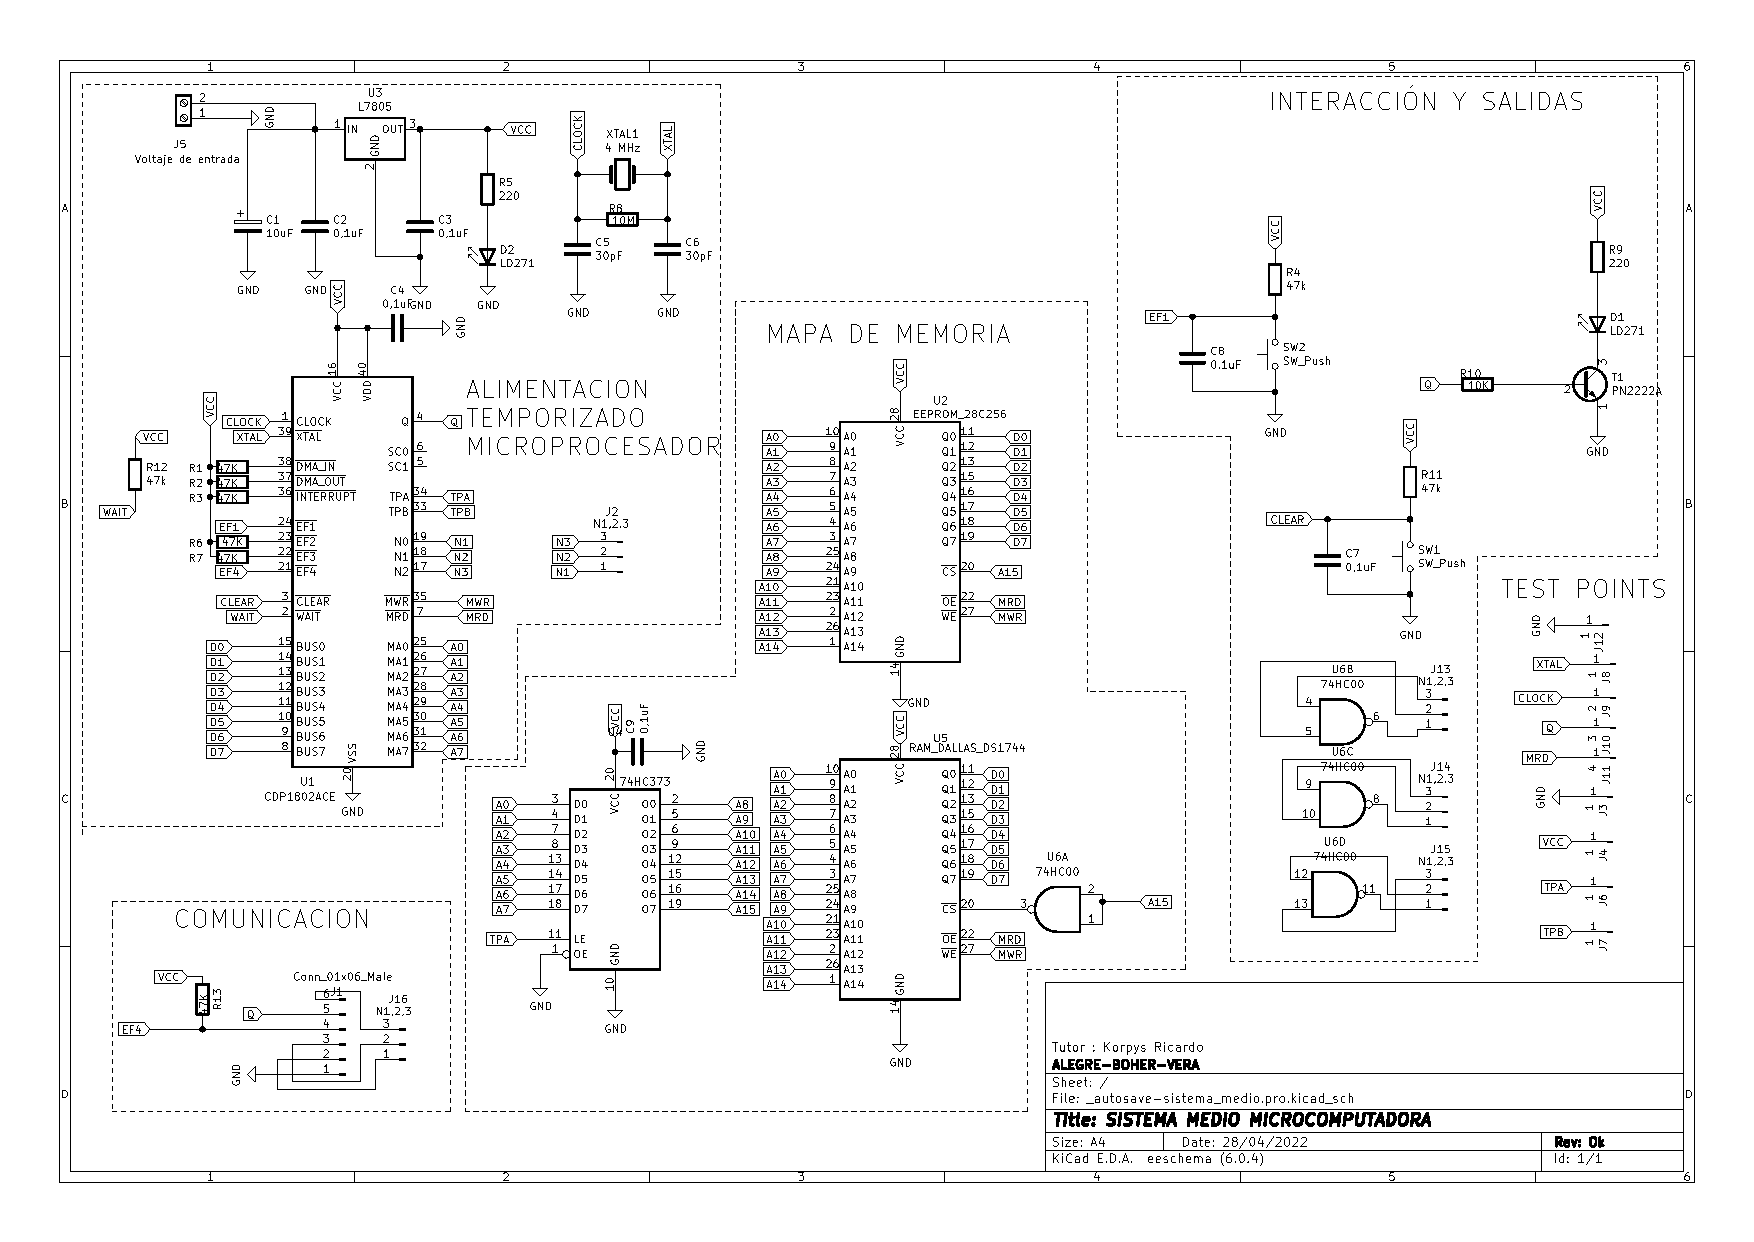
\includegraphics[width=1.20\textwidth, angle=90]{./imagenes/esquematico_SME.pdf}
  \caption{Esquemático del sistema medio}
  \label{F:esquematico_SME}
\end{figure}

 \begin{foto}[ht]
  \centering
  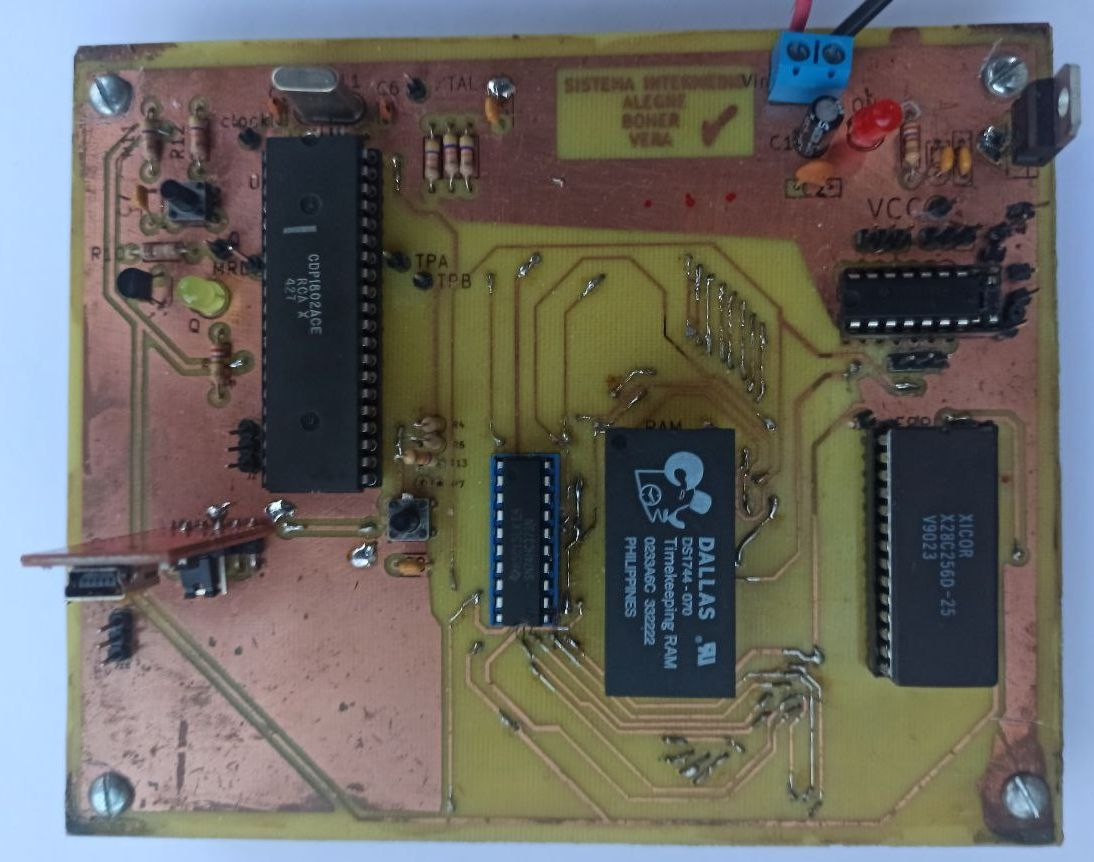
\includegraphics[width=0.9\textwidth]{./imagenes/foto_sistema_med.jpg}
  \caption{Sistema medio construido}
  \label{F:foto_sistema_med}
\end{foto}



\clearpage
\section{Lista de componentes}

En la tabla~\ref{T:bom_sis_med} se encuentra la lista de materiales para la construcción del sistema medio.

\begin{table}[ht!]
\caption{Lista de componentes del sistema medio}
\label{T:bom_sis_med}
\footnotesize
\begin{tabular}{|p{0.08\textwidth}|p{0.11\textwidth}|p{0.30\textwidth}|p{0.14\textwidth}|p{0.15\textwidth}|}
\hline
Cantidad & Etiqueta \newline
           Identificador            & Descripción                               & Fabricante            & Número de parte   \\ \hline \hline
1       & U1                        & Microprocesador                           & RCA                   & CDP1802ACE        \\ \hline
1       & U2                        & Memoria EEPROM 32k x 8                    & XICOR                 & X28C256D-25       \\ \hline
1       & U3                        & Regulador de tensión 5~\si{\volt}         & ST Microelectronics   & L7805CV          \\ \hline
1       & U4                        & Latch de 8 bits                           & Texas Instruments     & SN74HC373N        \\ \hline
1       & U5                        & Time keeping RAM 32K x8                   & Dallas                & DS1744-070        \\ \hline
1       & U6                        & Quadruple 2-Input NAND Gates              & Texas Instruments     & SN74HC00N         \\ \hline
1       & T1                        & Transistor BJT NPN                        & ST Microelectronics   & PN2222A           \\ \hline
1       & XTAL1                     & Cristal \num{4}~\si{\mega\hertz}          & CQ Electronics        & \listaVacio                \\ \hline
2       & SW1, SW2                  & Pulsador 6mm~x~4,3mm                      &  \listaVacio                     &  \listaVacio               \\ \hline
9      & R1, R2, R3, R4, R6, R7, R11, R12, R13
                                    & Resistor 47~\si{\kilo\ohm} 1/8~\si{\watt} &     \listaVacio                  &     \listaVacio            \\ \hline
2       & R5, R9                        & Resistor 220~\si{\ohm} 1/4~\si{\watt}     &      \listaVacio                 &   \listaVacio              \\ \hline
1       & R8                        & Resistor 10~\si{\mega\ohm} 1/8~\si{\watt} &    \listaVacio                   &      \listaVacio           \\ \hline
1       & R10                       & Resistor 10~\si{\kilo\ohm} 1/8~\si{\watt} &  \listaVacio                     &    \listaVacio             \\ \hline
1       & D1                        & LED Rojo 5mm                              &  \listaVacio                     &  \listaVacio               \\ \hline
1       & D2                        & LED Verde 5mm                             &   \listaVacio                    &  \listaVacio               \\ \hline
1       & C1                        & Capacitor electrolítico 10~\si{\micro\farad} 25~\si{\volt}
                                                                                & \listaVacio                      &  \listaVacio               \\ \hline
6       & C2, C3, C4, C7, C8, C9    & Capacitor cerámico \num{0.10}~\si{\micro\farad} 50~\si{\volt}
                                                                                &  \listaVacio                     &   \listaVacio              \\ \hline
2       & C5, C6                    & Capacitor cerámico \num{30}~\si{\pico\farad} 50~\si{\volt}
                                                                                & \listaVacio                      & \listaVacio                \\ \hline
1       & J1                        & 1x6 Pines Conectores Macho \num{2.54}~mm  &  \listaVacio                     &   \listaVacio              \\ \hline
5       & J2, J13, J14, J15, J16    & 1x3 Pines Conectores Macho \num{2.54}~mm  &  \listaVacio                     &  \listaVacio               \\ \hline
9       & J3, J4, J6, J7, J8, J9, J10, J11, J12
                                    & Pin conector macho (1 \textit{Male Header Pin})
                                                                                &  \listaVacio                     &  \listaVacio               \\ \hline
1       & J5                        & Bornera 2 pines \num{5.08}~mm             &  \listaVacio                     &  \listaVacio               \\ \hline
1       & No aplica                 & Módulo conversor USB-Serial               & Future Technology Devices International & FT232RL \\ \hline
\end{tabular}
\normalsize
\end{table}


\clearpage
\section{Programas del sistema medio}
\label{C:programas_del_sistema_medio}

Los programas realizados para el sistema mínimo, expuestos en la sección~\ref{C:ProgramasSMin}, son compatibles con el sistema medio, salvo el programa número~4, que requiere un ajuste en el contador utilizado para la rutina de retardo, debido a que el sistema medio utiliza un cristal de 4~\si{\mega\hertz} ($ T_{reloj} = \num{250}~\si{\nano\second} $), distinto al utilizado en el sistema mínimo. Para su cálculo, utilizamos la ecuación~\eqref{eq:contador}, expuesta en la sección~\ref{C:ComunicacionSerial}, y considerando, al igual que en el sistema mínimo, 600~baudios (Retardo = \num{0.001666667}~\si{\second}).

\begin{equation}
    CONT1BT = \frac{Retardo}{48\:T_{reloj}}-\frac{4}{3} = \frac{\num{0.001666667}~\si{\second}}{48\cdot\num{250}~\si{\nano\second}}-\frac{4}{3} = \num{137.56}\approx\num{138}
    \label{eq:calculo-1-bit-time-sistema-med}
\end{equation}

A continuación, se exponen otros programas implementados en el sistema medio.

\subsection{Intérprete Tiny Basic}

En la página oficial del Membership Card\cite{membership-card} puede encontrarse un intérprete Basic bajo el nombre de Tiny BASIC. El mismo tiene documentación y el código fuente, lo cual resulta de gran ayuda. Sin embargo, para su correcto funcionamiento en el sistema medio, es necesario realizar una serie de modificaciones en el código fuente.

La primera de estas modificaciones es en el archivo \texttt{1802reg.asm}, el cual contiene definido el nombre de los registros de trabajo. Sin embargo, faltaban algunos registros y fue necesario agregarlos. Para que el código pueda ser ensamblado sin errores, es necesario que este archivo tenga todas las definiciones que se encuentran en el código del listado~\ref{L:1802reg}.

\clearpage
\footnotesize
\lstinputlisting[language=CDP1802, caption={\centering Archivo \texttt{1802reg.asm} con definición de etiquetas para los registros de trabajo}, label = {L:1802reg}]{codigo/1802reg.asm}
\normalsize

Las siguientes modificaciones se realizaron sobre el código fuente del intérprete Tiny BASIC, más específicamente, el archivo \texttt{tb0\_test.asm}. Este código es muy extenso para ser incluido en este informe, sin embargo, se incluyen segmentos pequeños del código, donde pueden visualizarse las modificaciones realizadas.

La segunda modificación fue realizada en la línea 25, que puede verse en el listado~\ref{L:basic_mod1_starts_at_1}, donde la etiqueta \texttt{QHI} debe ser definida como 0, esto es necesario para que la línea de transmisión serial a través del pin Q, cuando esté en reposo, sin trasmitir datos, permanezca en estado alto, como lo establece el protocolo UART. Y la última modificación realizada, esta vez en la línea 28 del listado~\ref{L:basic_mod1_starts_at_1}, fue definir la etiqueta \texttt{AUTORUN} como 0; si esta etiqueta permanece definida como 1, al iniciar el intérprete, se ejecuta un código predefinido, lo cual en ocasiones resulta molesto, por lo que se decidió desactivar esta opción.

\footnotesize
\lstinputlisting[language=CDP1802, caption={\centering Segmento del código fuente \texttt{tb0\_test.asm} con modificación en línea 25 y 28}, label = {L:basic_mod1_starts_at_1}]{codigo/basic_mod1_starts_at_1.asm}
\normalsize

Estas son todas las modificaciones realizadas. Sin embargo, existen partes de interés en el código que vale la pena mencionar, a pesar de que no fueron modificadas. La primera de ellas se encuentra en la línea~91 del código, listado~\ref{L:basic_mod2_starts_at_89}, donde se encuentra definida la etiqueta \texttt{PAGE}, que define la posición de la memoria RAM en el mapa de memoria, empezando en este caso a partir de 8000~hexadecimal. Para el funcionamiento en el sistema medio no es necesario modificar esta etiqueta, sin embargo, en otras arquitecturas sí puede ser necesario.

\clearpage
\footnotesize
\lstinputlisting[language=CDP1802, caption={\centering Segmento del código fuente \texttt{tb0\_test.asm}, modificación de posición de memoria RAM en el mapa de memoria}, firstnumber=89, label = {L:basic_mod2_starts_at_89}]{codigo/basic_mod2_starts_at_89.asm}
\normalsize

Finalmente, en la línea~2194 del código, listado~\ref{L:basic_set_baudrate_starts_at_2187}, puede modificarse la velocidad de transmisión (baudrate). Por defecto es de \num{2400}~baudios para el caso del sistema medio, que utiliza un cristal de \num{4}~\si{\mega\hertz}.

\footnotesize
\lstinputlisting[language=CDP1802, caption={\centering Segmento del código fuente \texttt{tb0\_test.asm}, definición del baudrate utilizado con cristal de \num{4}~\si{\mega\hertz}}, firstnumber=2187, label = {L:basic_set_baudrate_starts_at_2187}]{codigo/basic_set_baudrate_starts_at_2187.asm}
\normalsize

\subsection{Sistema operativo ElfOS sin disco}

En la página oficial del Membership Card\cite{membership-card} puede encontrarse una versión del sistema operativo ElfOS sin disco (en la página el término en inglés es \entreComillas{Diskless Elf/OS ROM}). Desafortunadamente, el código fuente de este programa no se encuentra disponible, solo un archivo \texttt{.hex}. Esto significa que no es posible modificar el programa, pero puede ser grabado en una memoria y utilizado en el sistema medio.

Este sistema operativo inicia presentando un menú donde puede seleccionarse una serie de programas, en la figura~\ref{F:menu_del_elfOS} pueden visualizarse todos los programas disponibles.

 \begin{figure}[ht]
  \centering
  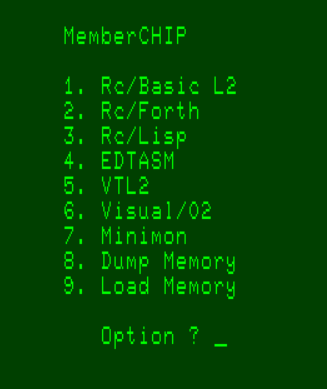
\includegraphics[width=0.35\textwidth]{./imagenes/menu_del_elfOS.png}
  \caption{Menú del sistema operativo ElfOS sin disco}
  \label{F:menu_del_elfOS}
\end{figure}

\clearpage
\section{Simulación Emma02}

\subsection{Intérprete Tiny Basic}

El intérprete Tiny Basic fue ejecutado correctamente en el simulador Emma02, utilizando el Membership Card, en la figura~\ref{F:config_emma_sis_med} puede apreciarse la configuración utilizada. Algo a ser destacado es que para la transmisión serial de datos, la configuración utilizada en el simulador es de 8 bits para el dato y sin bit de paridad, sin embargo, utilizando el sistema medio construido, se encontró que la configuración debe ser distinta; esta configuración se encuentra detallada en la sección~\ref{C:int_basic_resul_exper}.

 \begin{figure}[ht]
  \centering
  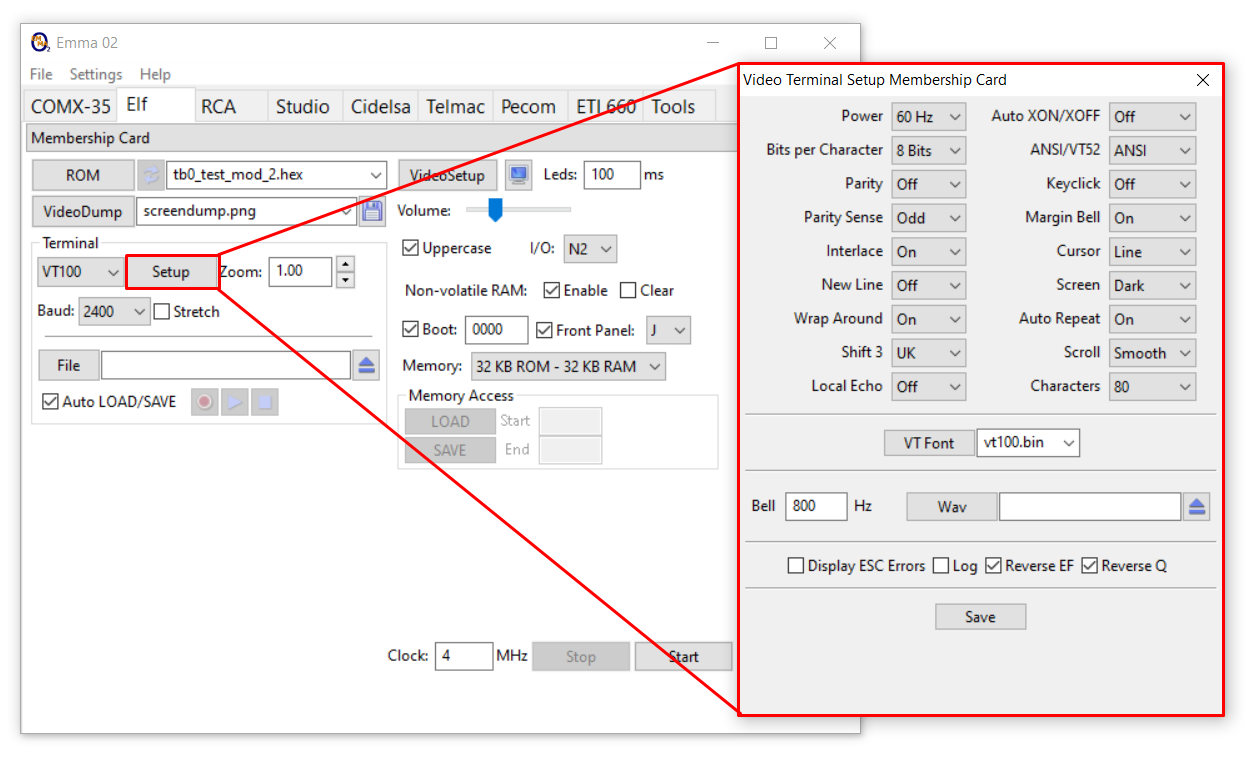
\includegraphics[width=1\textwidth]{./imagenes/config_emma_sis_med.png}
  \caption{\centering Configuración utilizada en el simulador Emma02 para ejecutar el intérprete Tiny Basic y el ElfOS sin disco}
  \label{F:config_emma_sis_med}
\end{figure}

\subsection{Sistema operativo ElfOS sin disco}

El sistema operativo ElfOS sin disco también fue ejecutado correctamente en el simulador Emma02, de nuevo utilizando el Membership Card con la misma configuración expuesta en la figura~\ref{F:config_emma_sis_med}.

\section{Resultados experimentales}

\subsection{Intérprete Tiny Basic}
\label{C:int_basic_resul_exper}

El intérprete Basic fue probado en el sistema medio, habiendo obtenido los mismos resultados que con el simulador Emma02. Sin embargo, para poder funcionar correctamente, fue necesario utilizar una configuración distinta para la comunicación serial. A continuación, se describe la misma.

Para la comunicación serial se utilizó una velocidad de 2400~baudios, 7 bits para los datos, bit de paridad impar y dos bits de stop, Flow Control en none, y transmit delay nulo.


\subsection{Sistema operativo ElfOS sin disco}

El sistema operativo ElfOS sin disco pudo ejecutarse correctamente en el sistema medio. La configuración para la comunicación serial fue la siguiente: Velocidad de 2400~baudios, 8~bits para los datos, sin bit de paridad y dos bits de stop, Flow Control en none, y transmit delay nulo.

\chapter{Sistema Final}

El sistema final es la culminación de los sistemas desarrollados en este proyecto, el cual parte del planteado para el sistema medio agregando funcionalidades extras al sistema que se detallarán más adelante. El mismo se encuentra planteado de manera que presente retrocompatibilidad, es decir, que todo software diseñado tanto para el sistema mínimo como para el sistema medio, debe funcionar en el sistema final. En comparación al sistema medio, se presentan la integración de la fuente de alimentación al sistema, el uso de memorias seriales, sistema de conversión AD, una interfaz de entrada salida expandida y un sistema de comunicación SPI.   
El circuito del sistema se encuentra diseñado, se presenta el esquemático, lista de componentes y diseño de placa PCB. No obstante, al momento de la escritura de este informe, el mismo no ha sido construido.

\section{Esquemáticos}
\label{C:EsqSF}
A modo de simplificar el análisis y presentación del sistema, el esquemático del mismo se presenta de manera modular, comenzando con el esquema generalizado (Ver figura \ref{F:EsquemaSF}) en el cual se pueden ver todas las partes que componen al sistema, sin adentrarse en un funcionamiento específico, para luego en las siguientes secciones pasar a especificar su funcionamiento.
Principalmente en este esquema podemos observar la interconexión entre el microprocesador y los dispositivos o periféricos asociados.

\begin{figure}[ht]
  \centering
  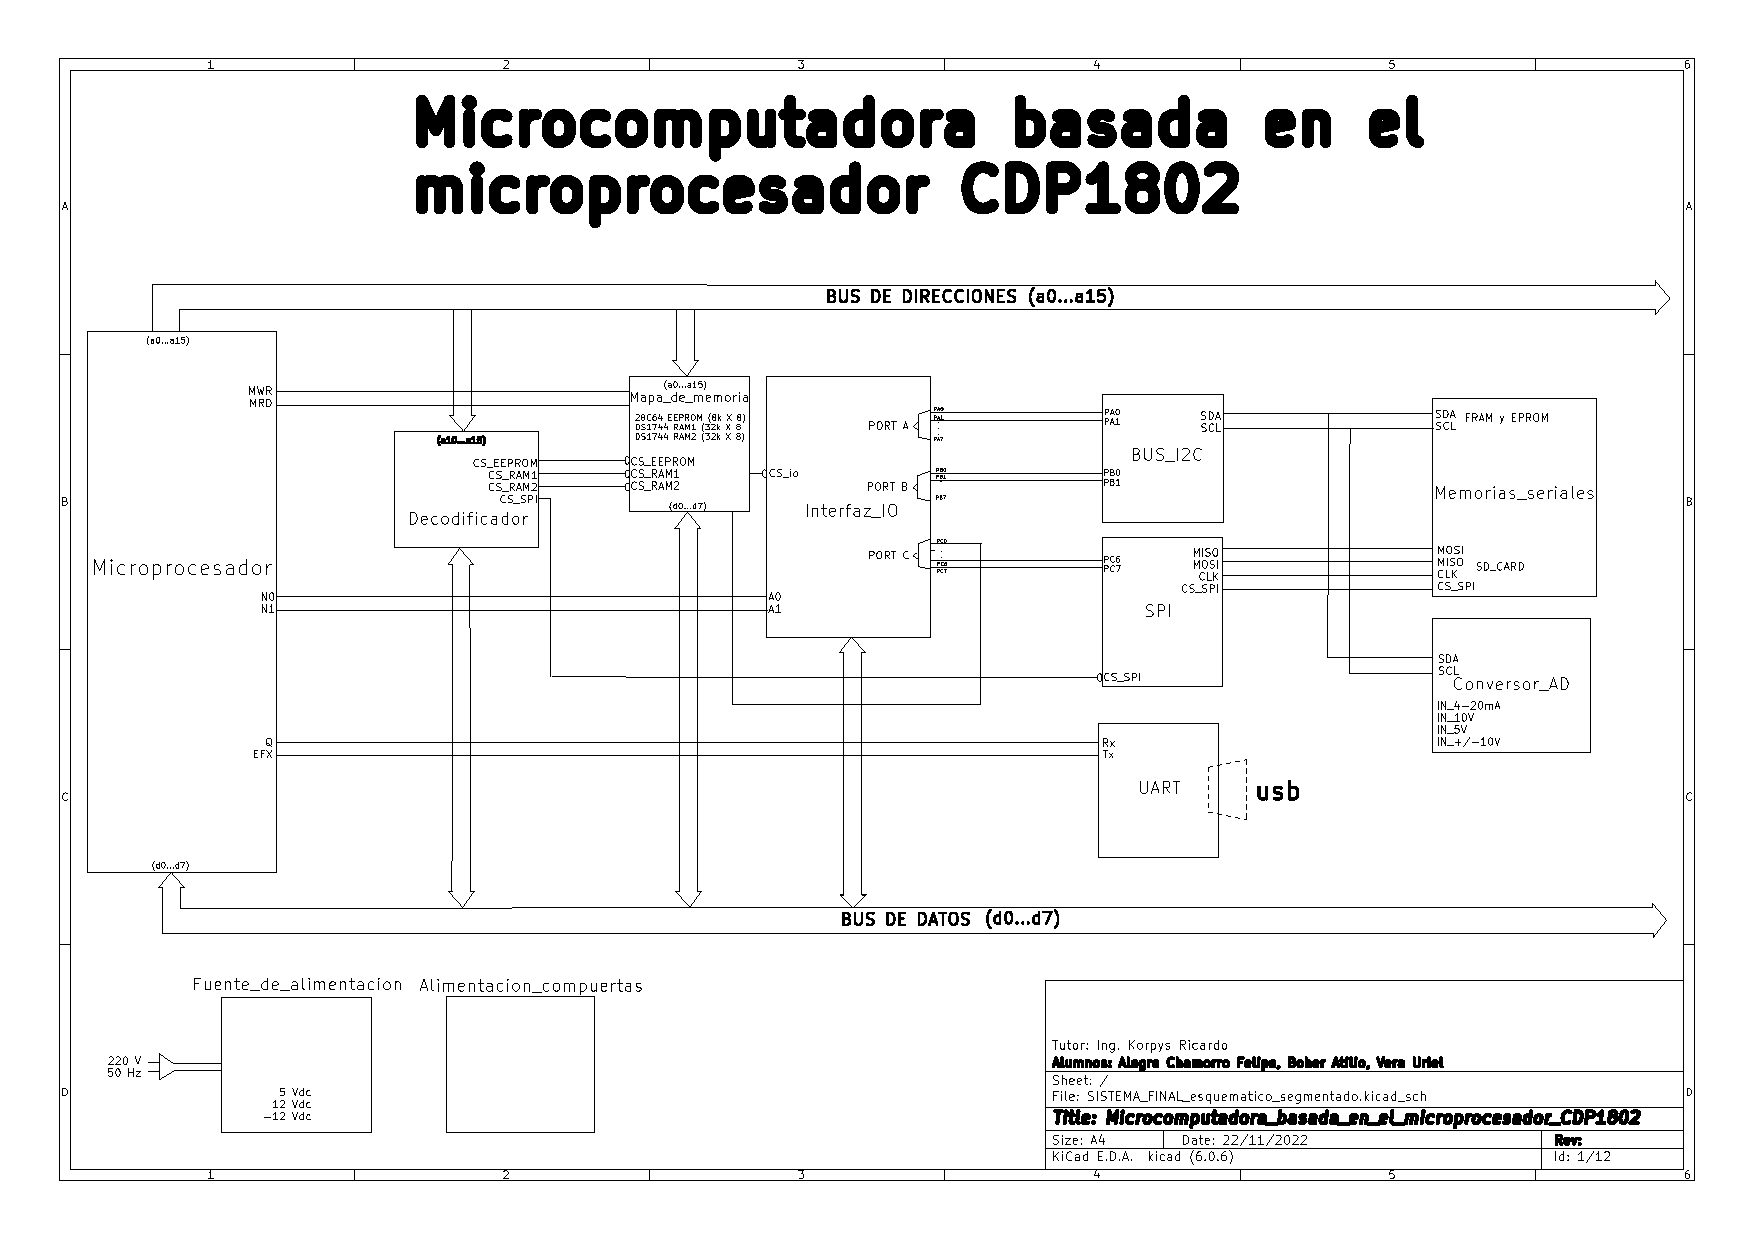
\includegraphics[width=1.2\textwidth, angle=90]{./imagenes/EsquematicosSF/Esquematico (1).pdf}
  \caption{Esquema general de sistema final}
  \label{F:EsquemaSF}
\end{figure}

\clearpage
\subsection{Fuente de alimentación}
La fuente de alimentación utilizada es lineal, basada en un transformador de tensión con punto medio. Dispone de un filtro de línea lo que reduce la distorsión armónica introducida en la red. 
Luego del proceso de rectificación y filtrado, se colocan etapas de regulación de tensión, para así poder alimentar los diferentes elementos del circuito que lo requieran. 

\begin{figure}[ht]
  \centering
  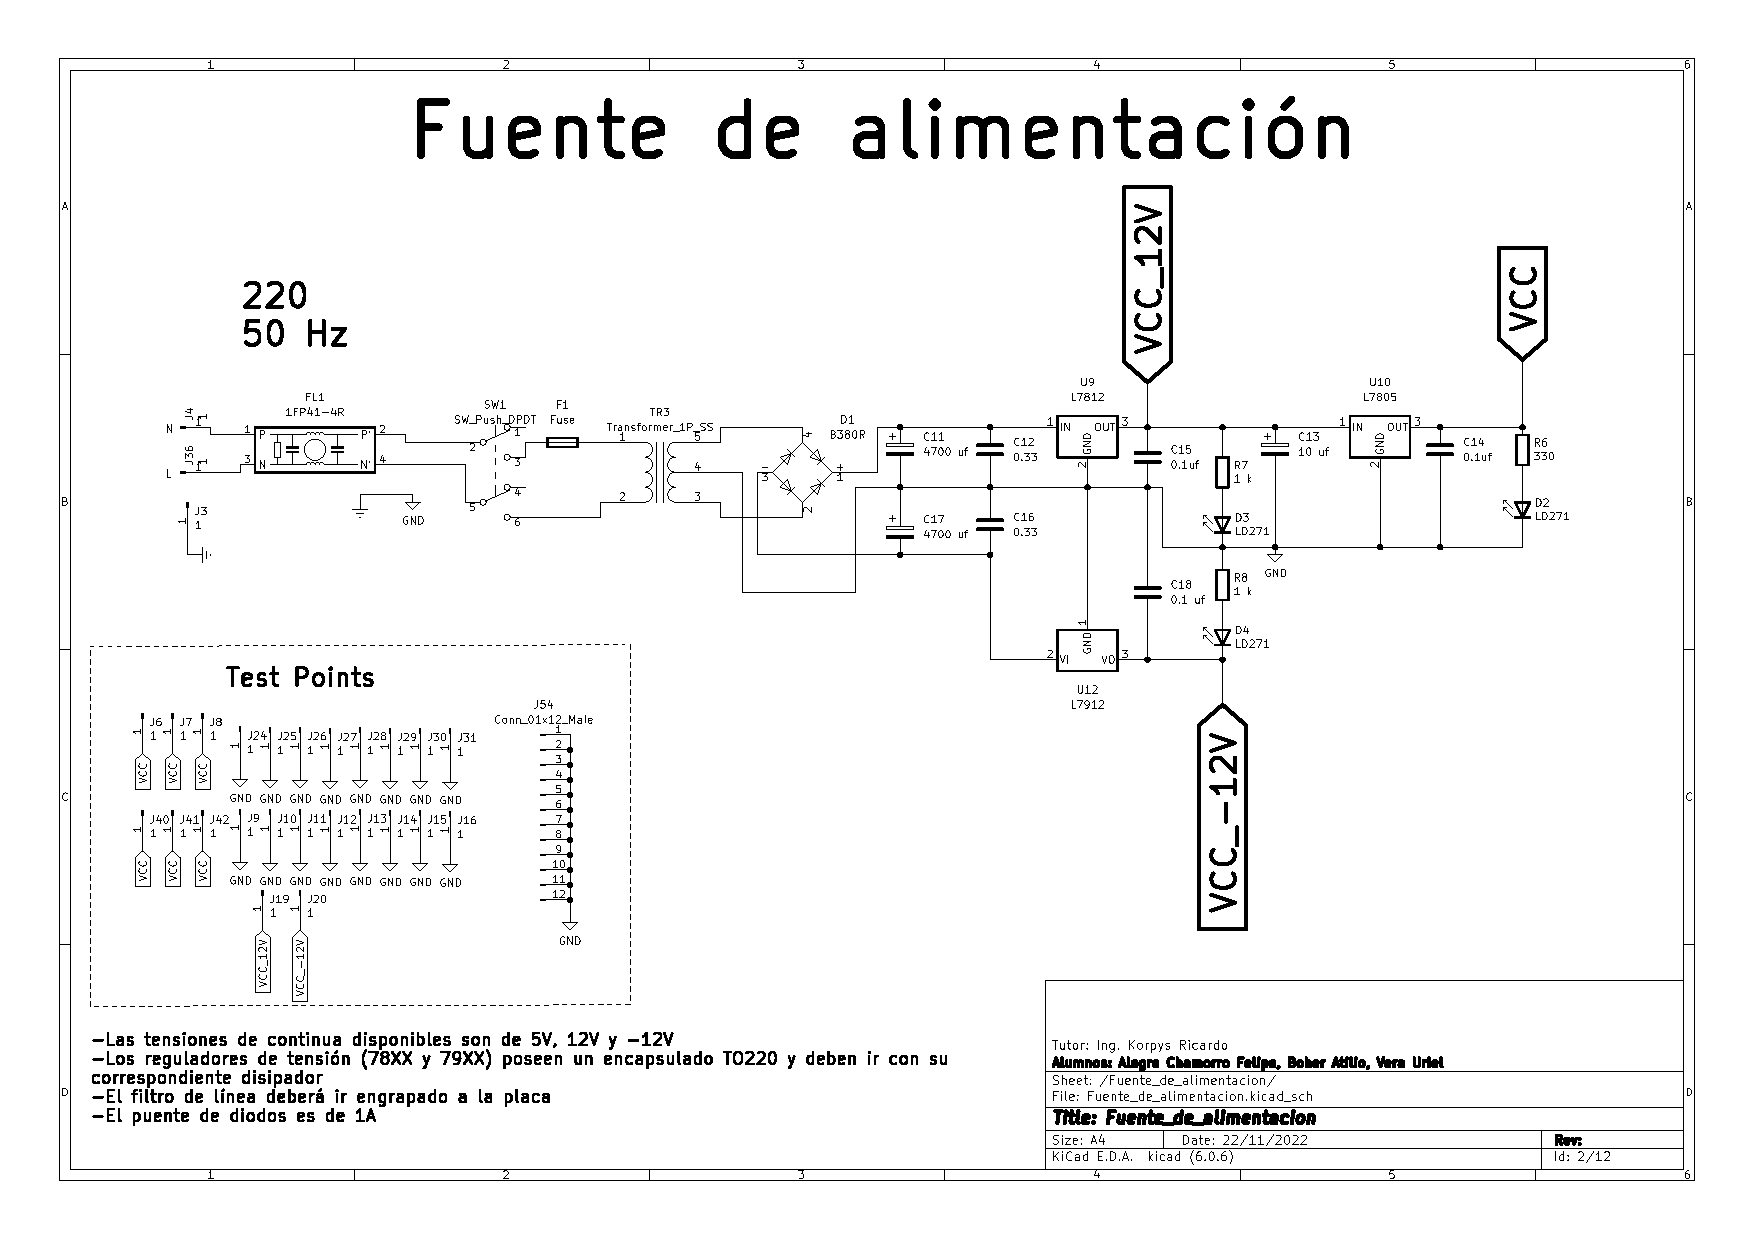
\includegraphics[width=1.2\textwidth, angle=90]{./imagenes/EsquematicosSF/Esquematico (2).pdf}
  \caption{Esquema de fuente de alimentación de sistema final}
  \label{F:EsqSF2}
\end{figure}

\clearpage
\subsection{Mapa de memoria}
El planteo establecido para el mapa de memoria consta de dos modos de operación, un modo de inicio y un modo de ejecución o RUN. El sistema fue pensado de esta manera para tener disponible más memoria RAM en ejecución. 

El modo inicio consiste en la memoria EEPROM 28C256 en la primera mitad del mapa de memoria (0000h a 7FFFh) y en la segunda mitad una memoria RAM en dos tramos de 8000h a F7FFh y luego continúa en FC00h hasta FFF8h, se interrumpe de esta manera la RAM para simplificar el circuito decodificador el cual se presenta más adelante (Sección \ref{C:Decodificador}). La sección del mapa de memoria de F800h hasta FBFFh es destinada a la comunicación SPI. Y finalmente, en la zona superior del mapa de memoria (FFF8h a FFFFh), la memoria RAM DALLAS 1744 posee un apartado para un reloj de tiempo real. 

El modo de ejecución es un modo en el cual se cambia la primera mitad del mapa de memoria (0000h a 7FFFh). El proceso consiste en cambiar la memoria EEPROM del modo de inicio por una memoria RAM. Este proceso debe ser ejecutado por software y para ello en el modo de inicio se debe copiar el contenido de la memoria EEPROM en la RAM1, luego el sistema seguirá funcionando con la memoria de programa en la RAM1 y en la primera mitad del mapa de memoria se tendrá disponible la memoria RAM2. 

\begin{figure}[ht]
  \centering
  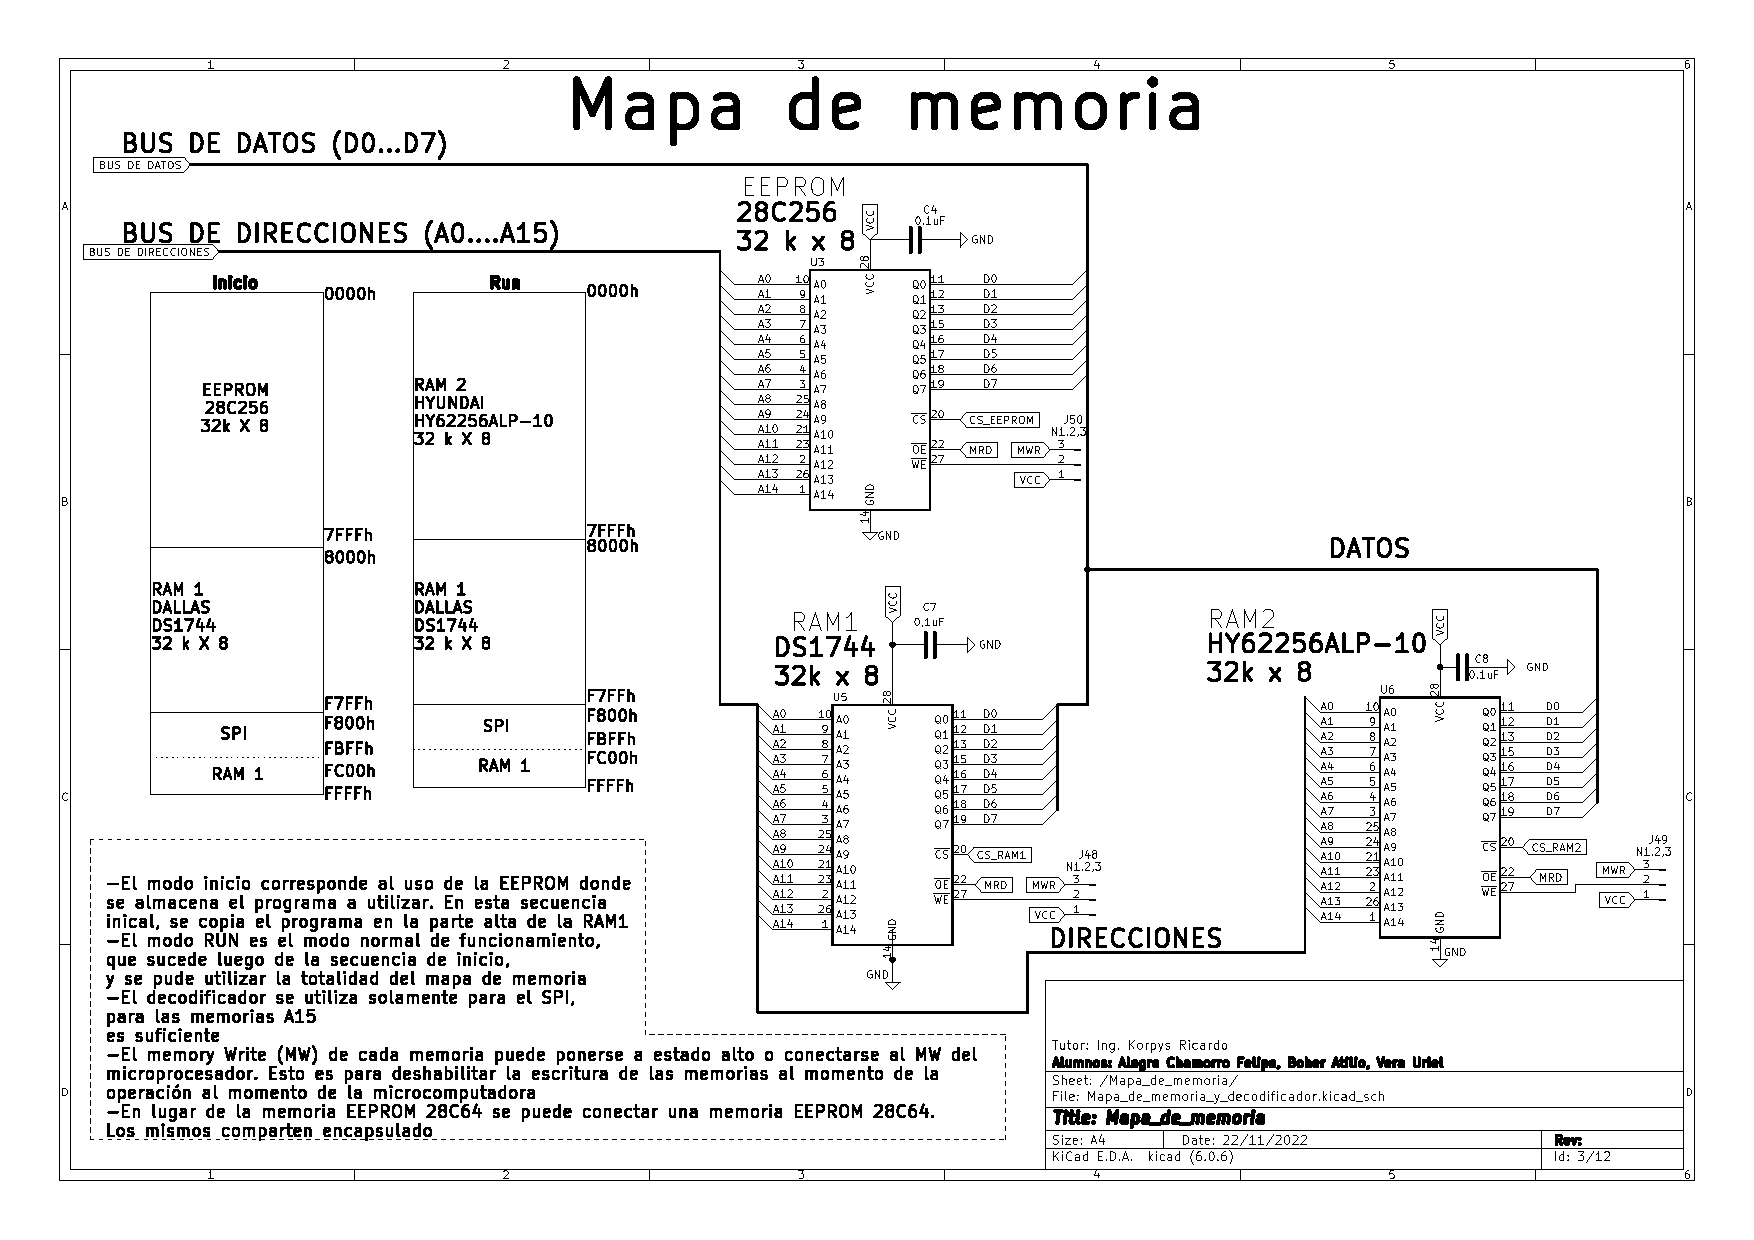
\includegraphics[width=1.2\textwidth, angle=90]{./imagenes/EsquematicosSF/Esquematico (3).pdf}
  \caption{Esquema de Mapa de memoria de sistema final}
  \label{F:EsqSF3}
\end{figure}

\clearpage
\subsection{Memorias seriales}
El trabajo con memorias seriales fue planteado para diferentes tecnologías de memorias, específicamente del tipo EEPROM, FRAM y SDcard. Para la comunicación I2C se prevé el uso de un sistema de comunicación por software utilizando la interfaz de entrada salida presentada en la sección \ref{C:I/O} e interactuando con el acondicionamiento presentado en \ref{C:BUSI2C}, mientras que para la comunicación SPI, se diseñó un sistema por hardware presentado en la sección \ref{C:esqSPI}. En el esquema de la figura \ref{F:EsqSF4} se observan las etiquetas de interconexión con el resto del circuito.
\begin{figure}[ht]
  \centering
  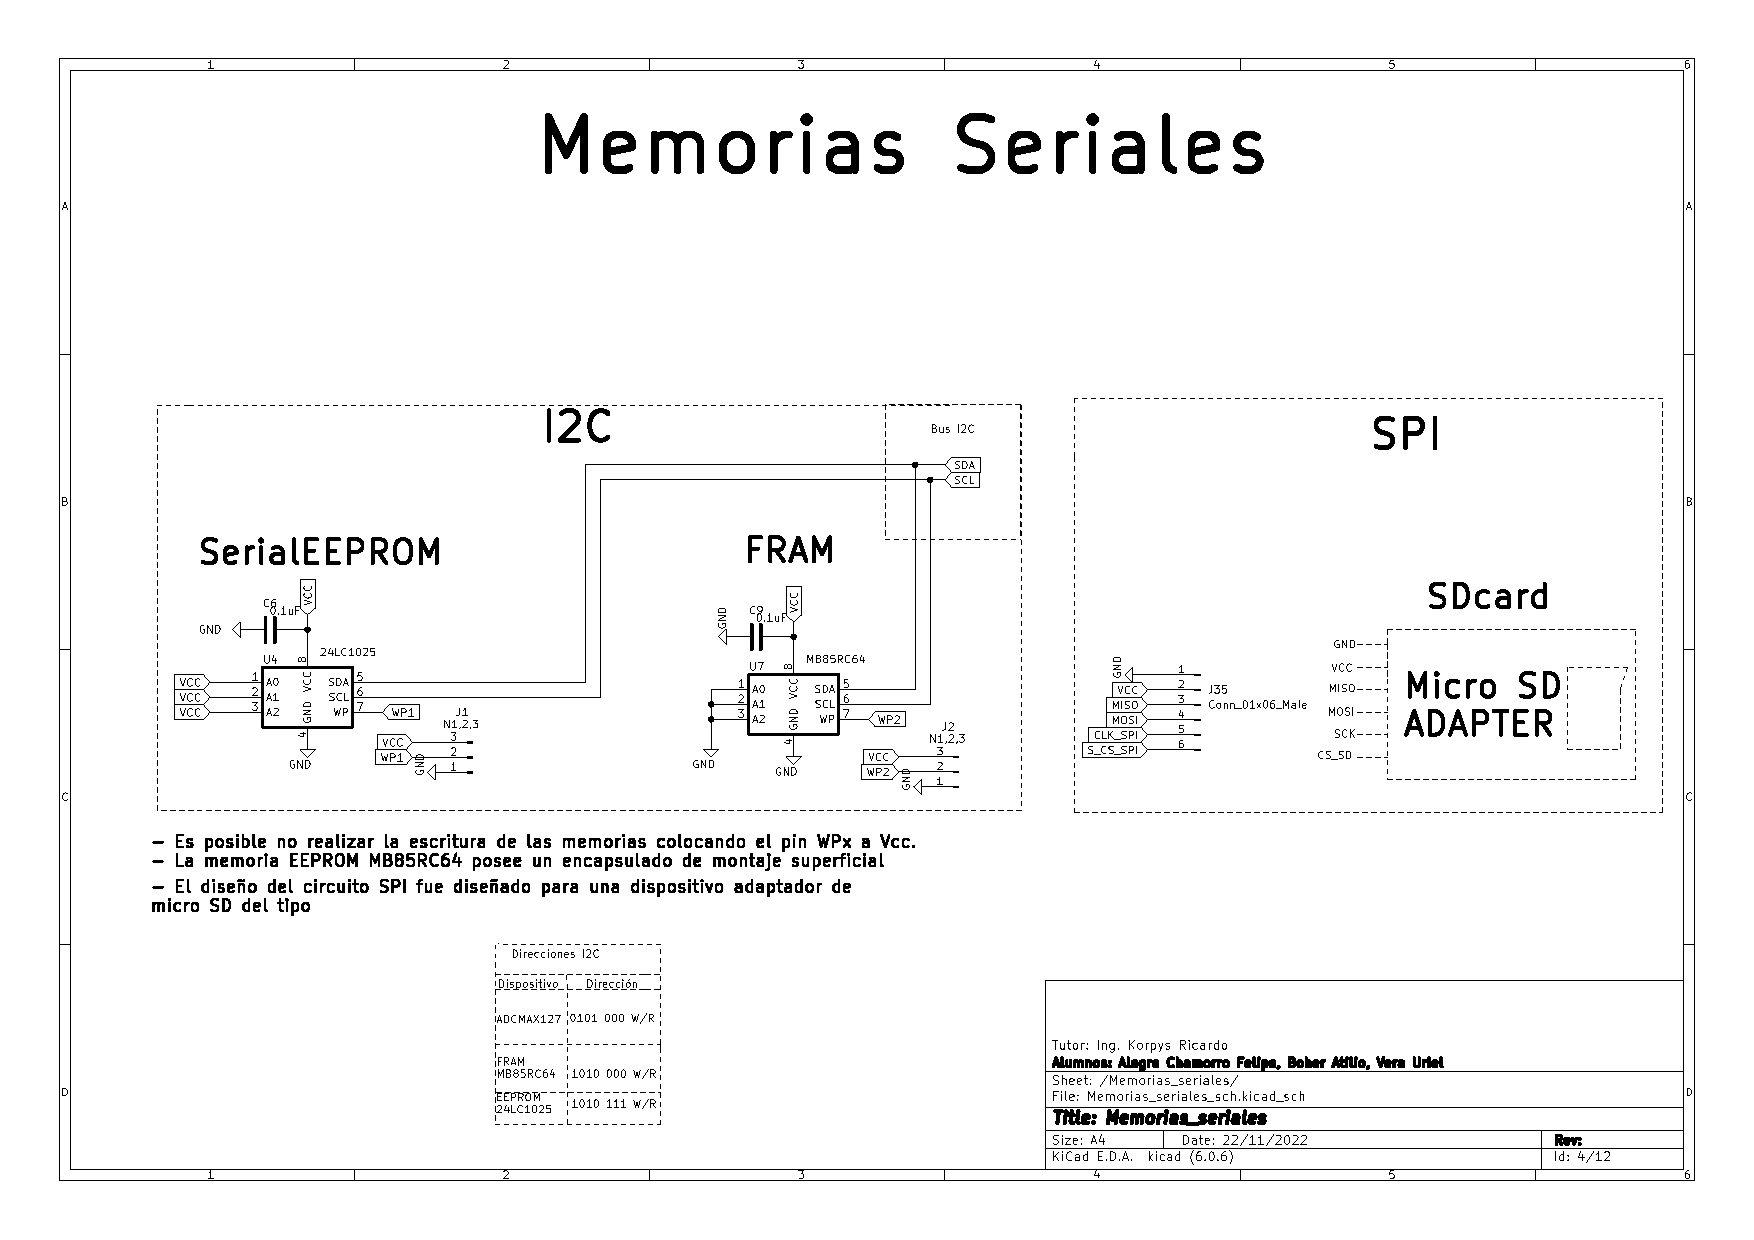
\includegraphics[width=1.2\textwidth, angle=90]{./imagenes/EsquematicosSF/Esquematico (4).pdf}
  \caption{Esquema de memorias seriales de sistema final}
  \label{F:EsqSF4}
\end{figure}

\clearpage
\subsection{Conversor analógico digital}

El sistema de conversión analógico-digital se basa en el MAX127 \cite{datasheet_max127}. Este conversor de 12 bits es configurable, lo que permite seleccionar el rango de tensiones a medir por cada canal y se realiza mediante comunicación I2C. Los rangos de medición pueden ser:
\begin{itemize}
    \item 0~V a 5~V
    \item -5~V a 5~V
    \item 0~V a 10~V
    \item -10~V a 10~V
\end{itemize}

Para el acondicionamiento de señal se utilizan amplificadores operacionales OPA4277~\cite{datasheet_OPA4277}. Los amplificadores operacionales se configuraron como conversores de corriente a tensión, de 4-20~mA a 0-10~V. Se concibió el diseño de esta manera, ya que en caso de que se requiera medir tensiones, el circuito puede ser modificado para que los amplificadores operacionales funcionen como seguidores de tensión. Basta con modificar el rango de medición por software para que la lectura refleje correctamente el valor a la entrada. 

\begin{figure}[ht]
  \centering
  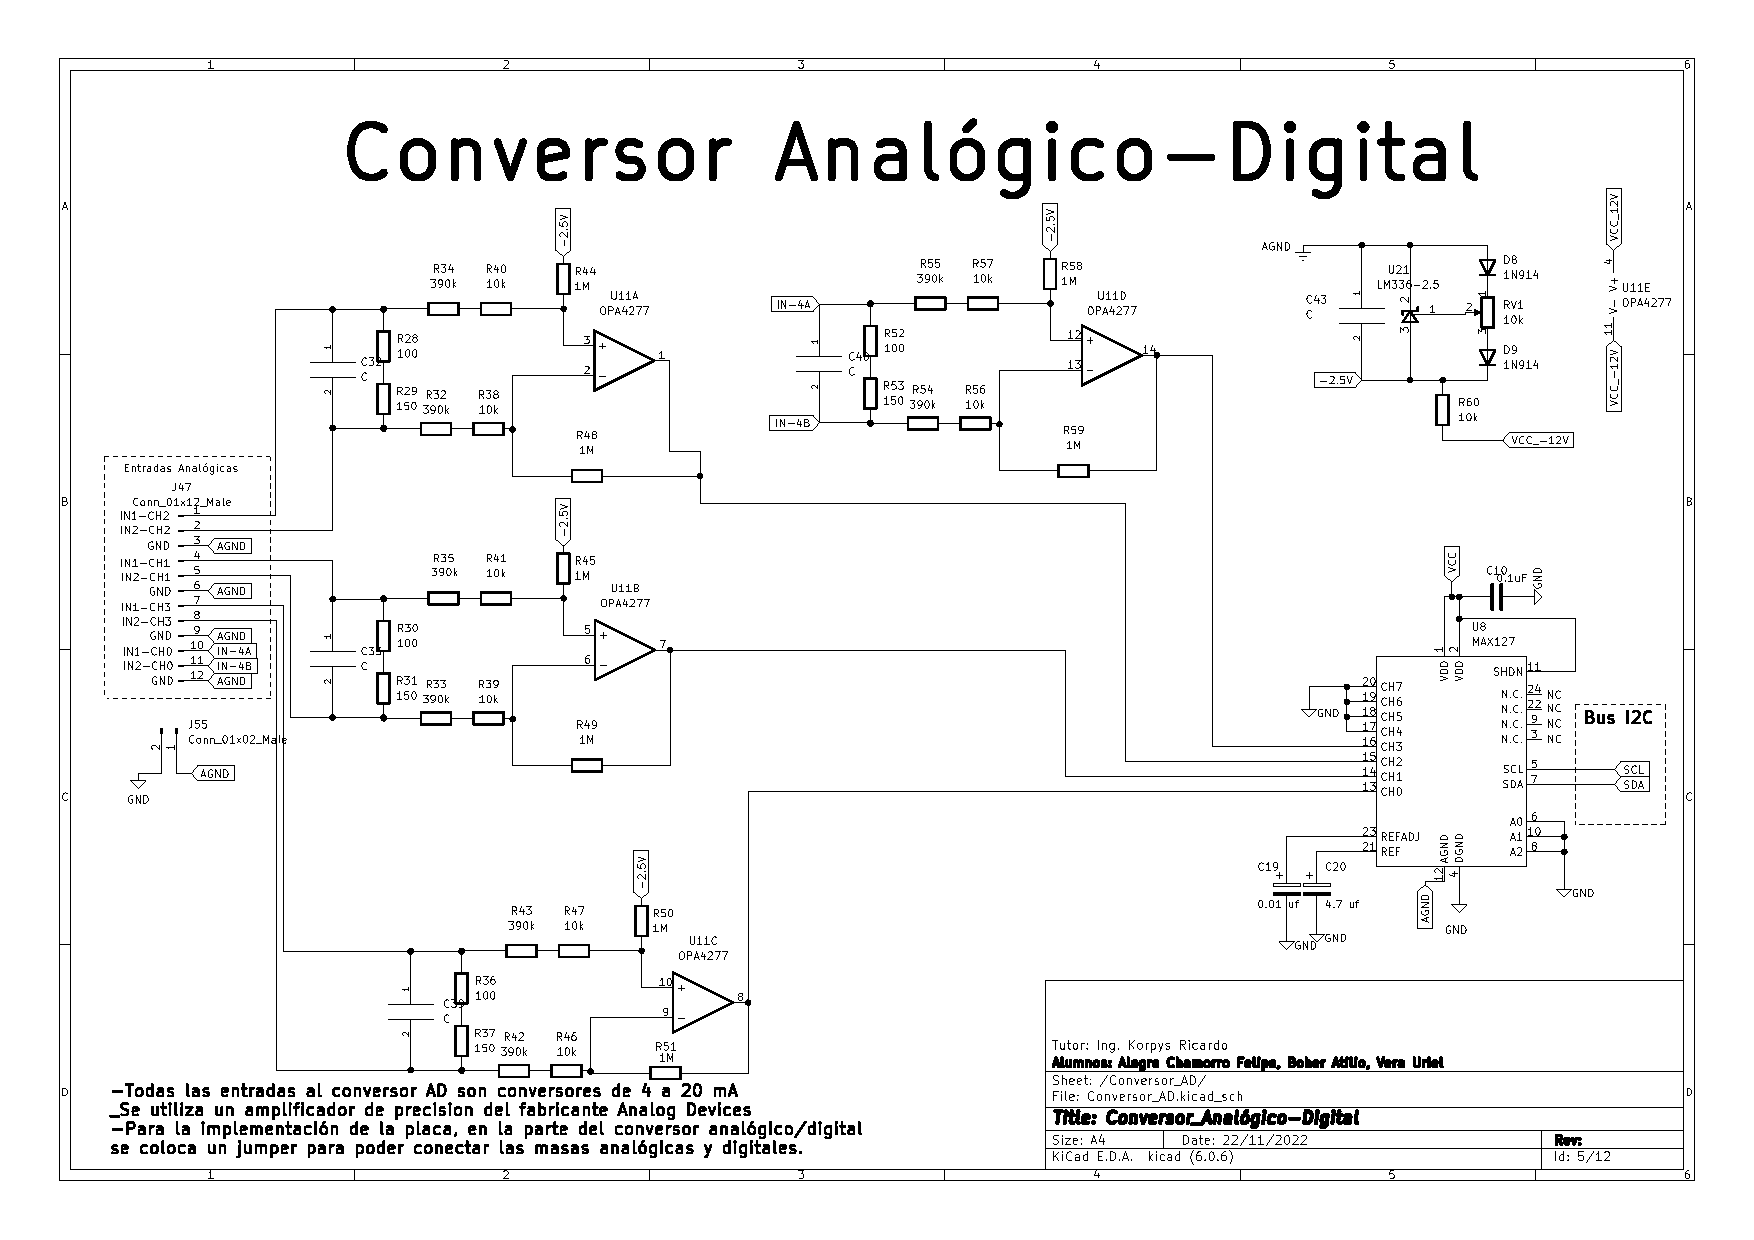
\includegraphics[width=1.2\textwidth, angle=90]{./imagenes/EsquematicosSF/Esquematico (5).pdf}
  \caption{Esquema de conversor analógico digital de sistema final}
  \label{F:EsqSF5}
\end{figure}

\clearpage
\subsection{Microprocesador}
En el esquema del microprocesador se observa su interacción con el resto del circuito. Es interesante destacar el latch 74HC573~\cite{datasheet_74HC573} el cual se encarga de transmitir los bits más significativos del bus de direcciones (A8-A15), esta configuración de microprocesador/latch para el direccionamiento es propia de la arquitectura propuesta por el CDP1802. Sin embargo, se utiliza un circuito integrado distinto al del sistema medio ya que su distribución de pines permite simplificar el diseño de la placa PCB. En el esquema también se puede observar una interfaz de usuario compuesta por pulsadores para señal de entrada y LEDs para señal de salida. 
El circuito oscilador que se presenta en el esquema está construido a partir de un cristal de 4~MHz. Es importante destacar que en la hoja de datos del microprocesador la frecuencia máxima para las condiciones de trabajo que establecemos es de 3,2~MHz, sin embargo, en la práctica es utilizado a mayor frecuencia y existen muchos casos prácticos que corroboran el funcionamiento con overclocking, como en la computadora Membership Card mencionada anteriormente \cite{membership-card}. 

\begin{figure}[ht]
  \centering
  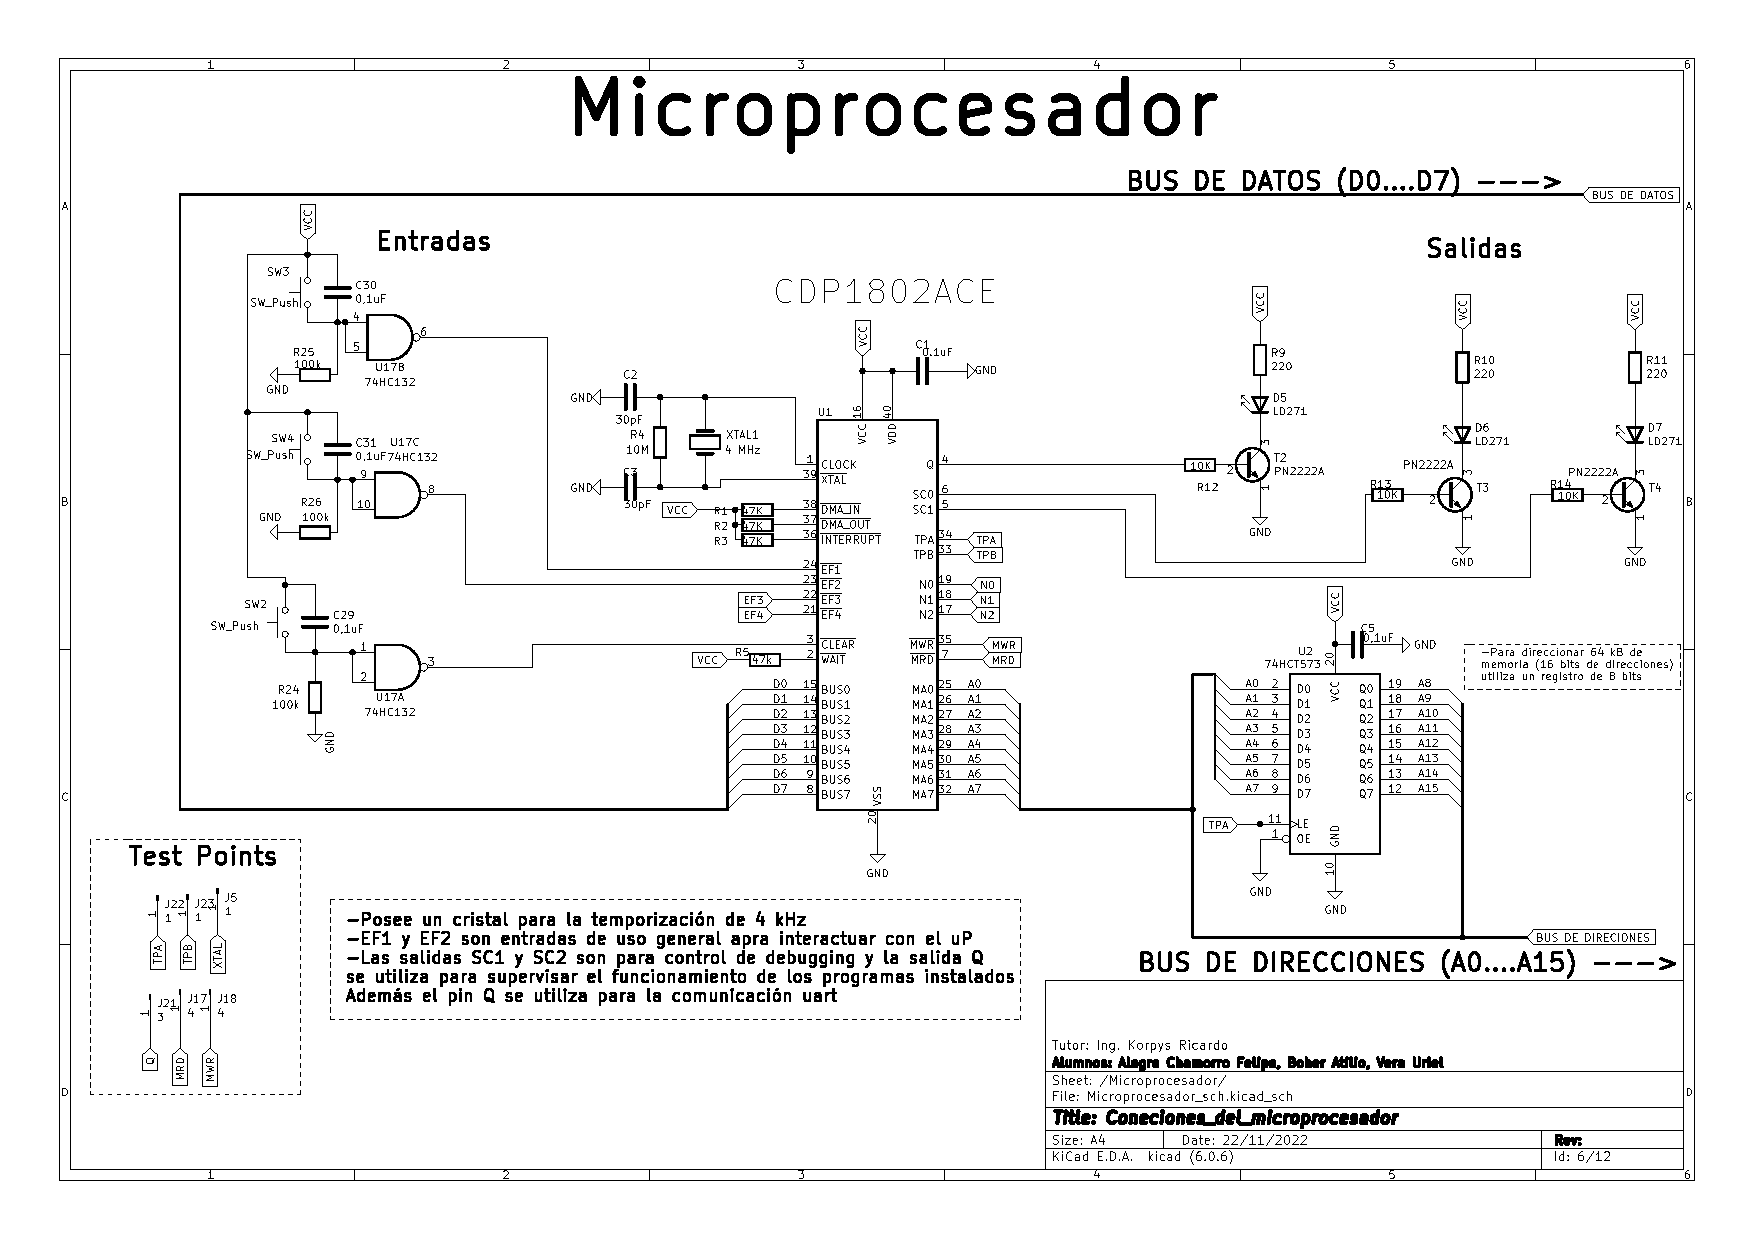
\includegraphics[width=1.2\textwidth, angle=90]{./imagenes/EsquematicosSF/Esquematico (6).pdf}
  \caption{Esquema de conexión de microprocesador de sistema final}
  \label{F:EsqSF6}
\end{figure}

\clearpage
\subsection{Decodificador}
\label{C:Decodificador}

El circuito decodificador se encarga de activar la selección de los dispositivos según lo presente en el bus de direcciones. Para ello se utiliza un circuito lógico con compuertas y un decodificador de 3 líneas a 8 líneas 74HC138 \cite{datasheet_74HC138}.

\begin{figure}[ht]
  \centering
  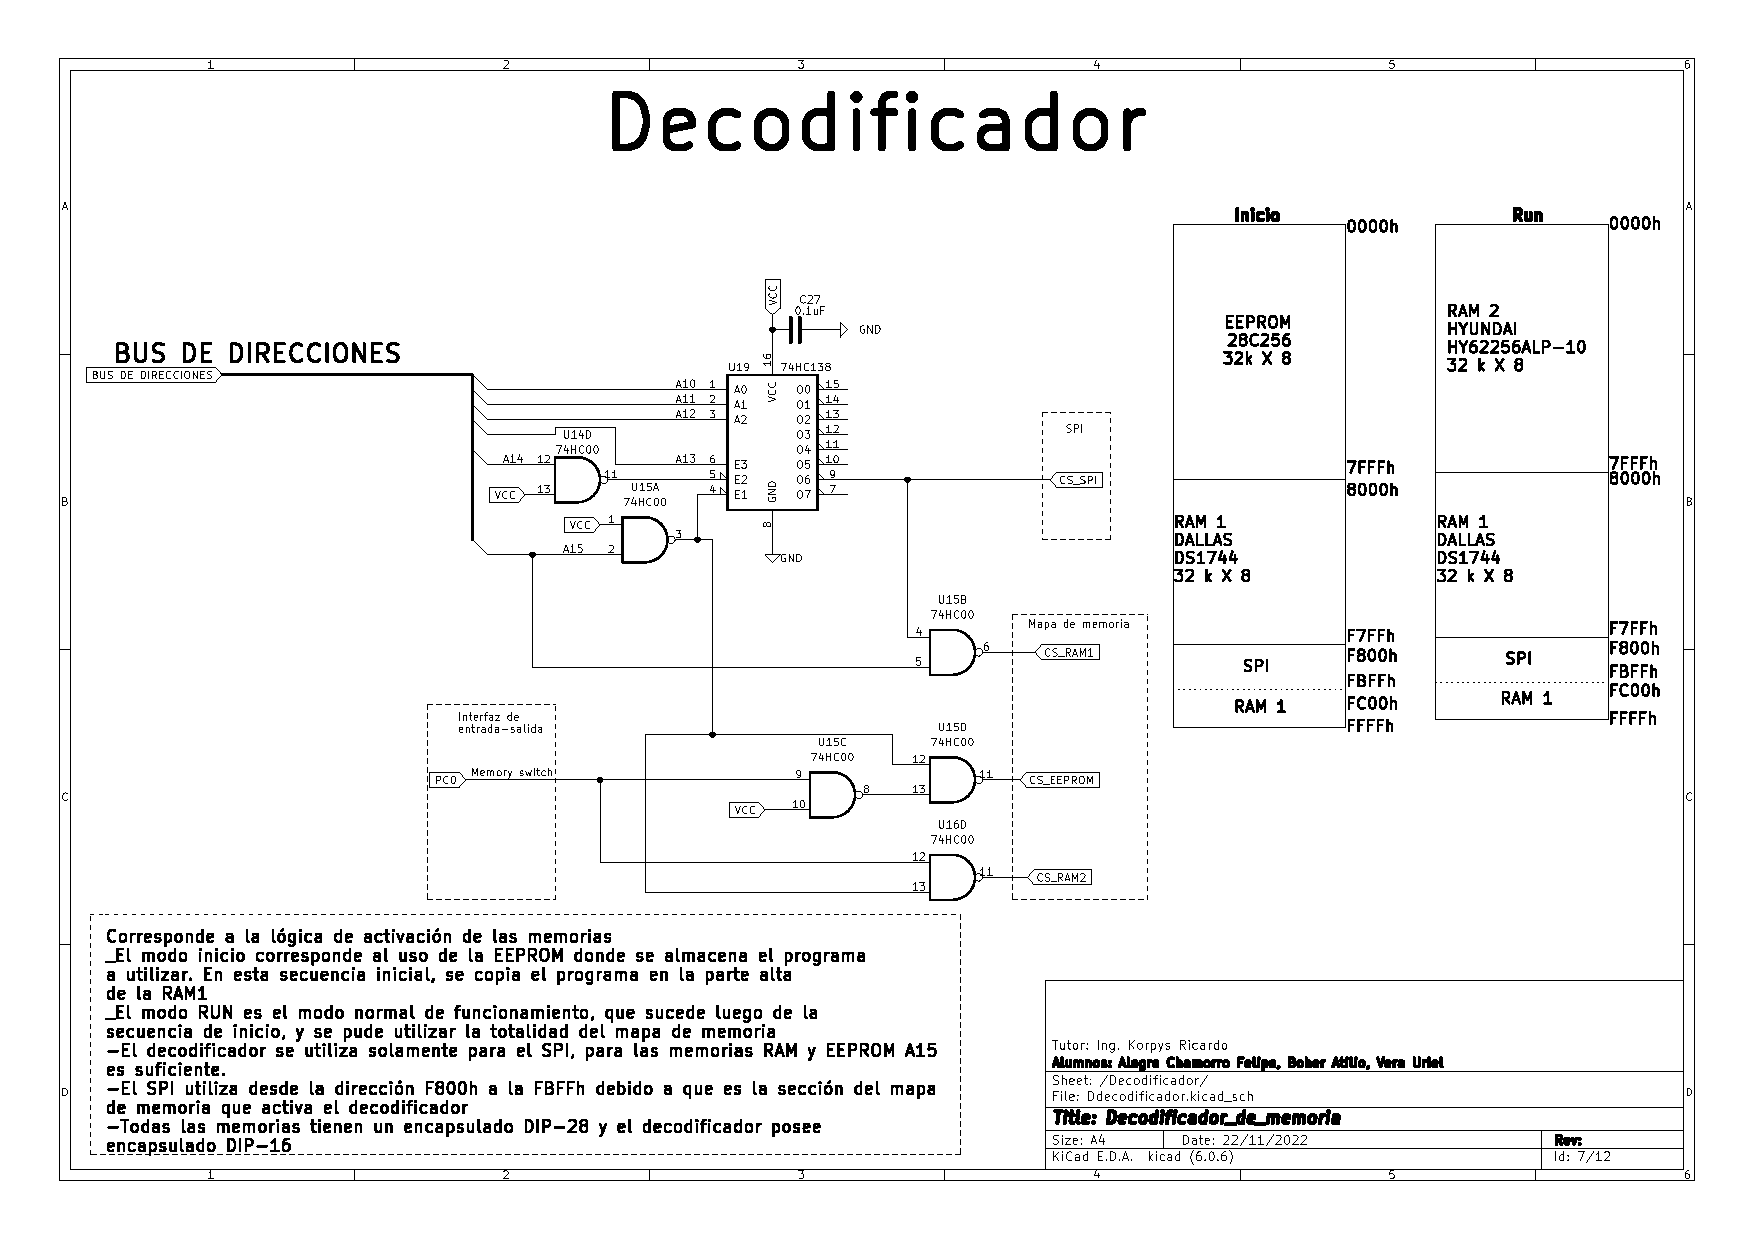
\includegraphics[width=1.2\textwidth, angle=90]{./imagenes/EsquematicosSF/Esquematico (7).pdf}
  \caption{Esquema de decodificador de memoria de sistema final}
  \label{F:EsqSF7}
\end{figure}

\clearpage
\subsection{Comunicación UART}

La comunicación UART se basa principalmente en el software que la controla y se utiliza el pin Q del microprocesador para la transmisión de datos. Para lograr establecer comunicación con una terminal en una computadora personal se requiere la conexión por medio de USB, por lo que se conecta una interfaz FT232RL~\cite{datasheet_FT232RL} que realiza la interpretación y retransmisión de los protocolos. 

\begin{figure}[ht]
  \centering
  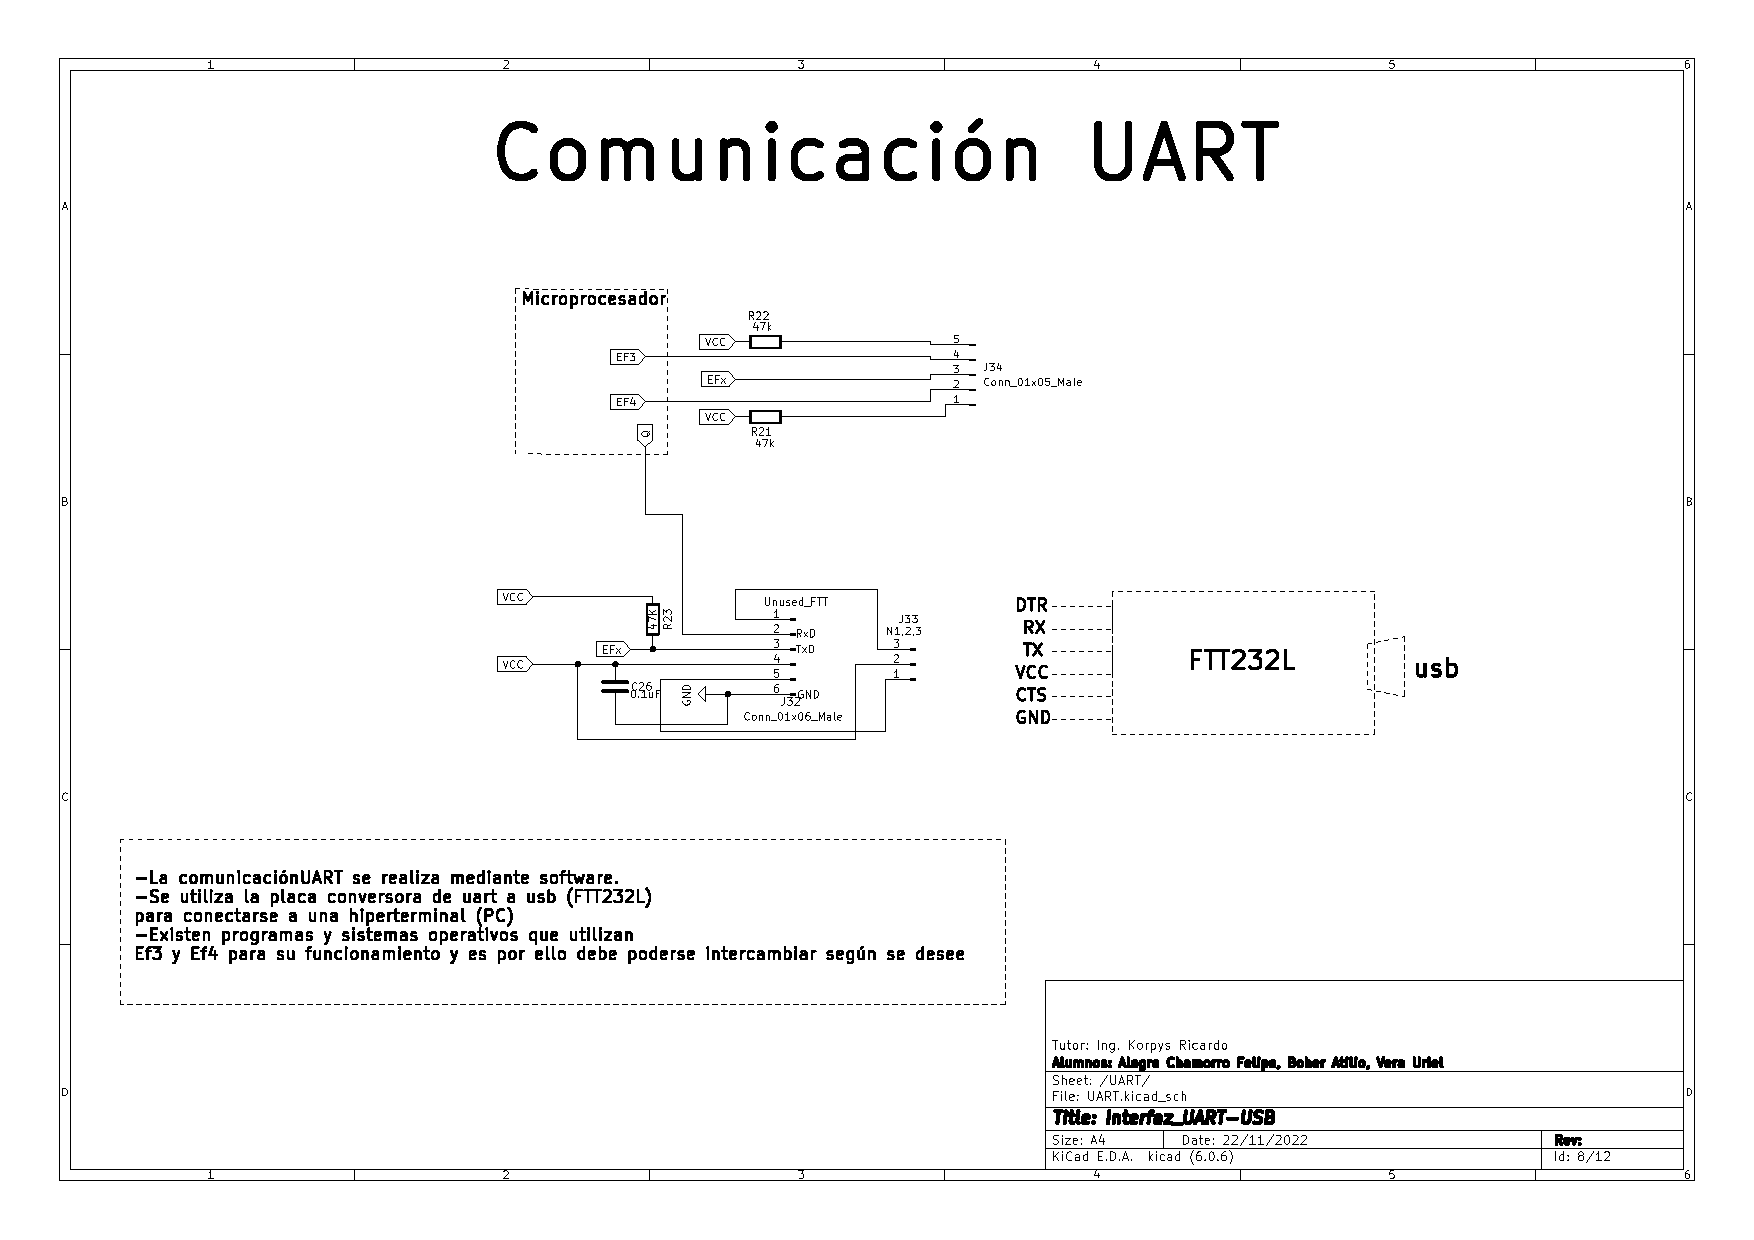
\includegraphics[width=1.2\textwidth, angle=90]{./imagenes/EsquematicosSF/Esquematico (8).pdf}
  \caption{Esquema de comunicación UART de sistema final}
  \label{F:EsqSF8}
\end{figure}

\clearpage
\subsection{Comunicación SPI}
\label{C:esqSPI}

En el esquemático de la figura~\ref{F:EsqSF9} se observa un circuito diseñado para realizar una comunicación basada en el protocolo SPI. Fue planteado con el objetivo de simplificar el procesamiento de datos en el microprocesador, realizándose un gran número de iteraciones en el circuito de manera transparente para el procesador. 

En principio se debe considerar que el sistema planteado cuenta con una señal de reloj proveniente de un cristal oscilador compatible con CMOS. Este cristal, al igual que el conectado al microprocesador, es de 4~MHz. Considerando que las instrucciones en el procesador duran 8 ciclos de reloj, se tendrá una velocidad de procesamiento mayor en el hardware diseñado. Esto se representa más adelante en los diagramas temporales. 

Básicamente el sistema presentado consiste en hacer trabajar 2 registros de desplazamiento (shift-register), uno para enviar datos y el otro para recibirlos. 

Para el envío de datos se utiliza un registro de desplazamiento de entrada paralela y salida serie, el MC14014 \cite{datasheet_MC14014B} (también se encuentra como CD4014). Este dispositivo cuenta con un registro interno el cual guarda el dato disponible en el bus al recibir una señal en estado alto en el pin PL. La lectura de los puertos de entrada se realiza con la señal de clock, por lo que para el guardado de los datos en el bus se debe detectar un flanco ascendente en el pin CP. Una vez guardado el dato en el registro, se encuentra listo para transmitirlo, este proceso se acciona con una señal de estado bajo en el pin PL y se transmite de manera serial con las transiciones positivas de la señal de reloj. 

Para la recepción de datos se utiliza un registro de desplazamiento de entrada serial y salida paralelo, el 74HC595 \cite{datasheet_74HC595}. Este dispositivo cuenta con una entrada serial, por la cual toma el dato a almacenar, realizando una lectura en dicha entrada por cada flanco de reloj detectado. El dato presente en el registro de desplazamiento varía por cada ciclo de reloj, por lo que al transcurrir 8 ciclos se encuentra completo el registro, para guardar este dato y que no se vea alterado por el transcurso de los posteriores ciclos, se utiliza el pin RCLK que permite guardar el dato en un registro paralelo. Para que este dato sea presentado en la salida paralelo, se pone en estado bajo el pin de output enable $\overline{\text{OE}}$.

La señal de clock utilizada para los integrados mencionados anteriormente se genera a partir del circuito establecido entre el cristal oscilador, el flip flop D 74HC74, el contador 74HC161 y el flip flop JK 74HC73 \cite{datasheet_74HC161, datasheet_74HC73, datasheet_74HC74}. La topología presentada en el esquema detecta el inicio del ciclo al recibir la señal proveniente de PC7, poniendo en estado alto el pin 4 del 74HC74, la señal generada por Q inicializa el contador. En el contador se toma la señal Q0 como señal de reloj, la cual tendrá una frecuencia de 2~MHz y luego cuando el contador se desborda la salida TC se pone en alto, esta señal es resguardada por el flip flop 74HC73 y utilizada como señal de reinicio del flip flop 74HC74. De esta manera se genera una señal oscilante de 2~MHz a la salida pero que solo tiene 8 pulsos, lo necesario para realizar el envío de un byte. 

\begin{figure}[ht]
  \centering
  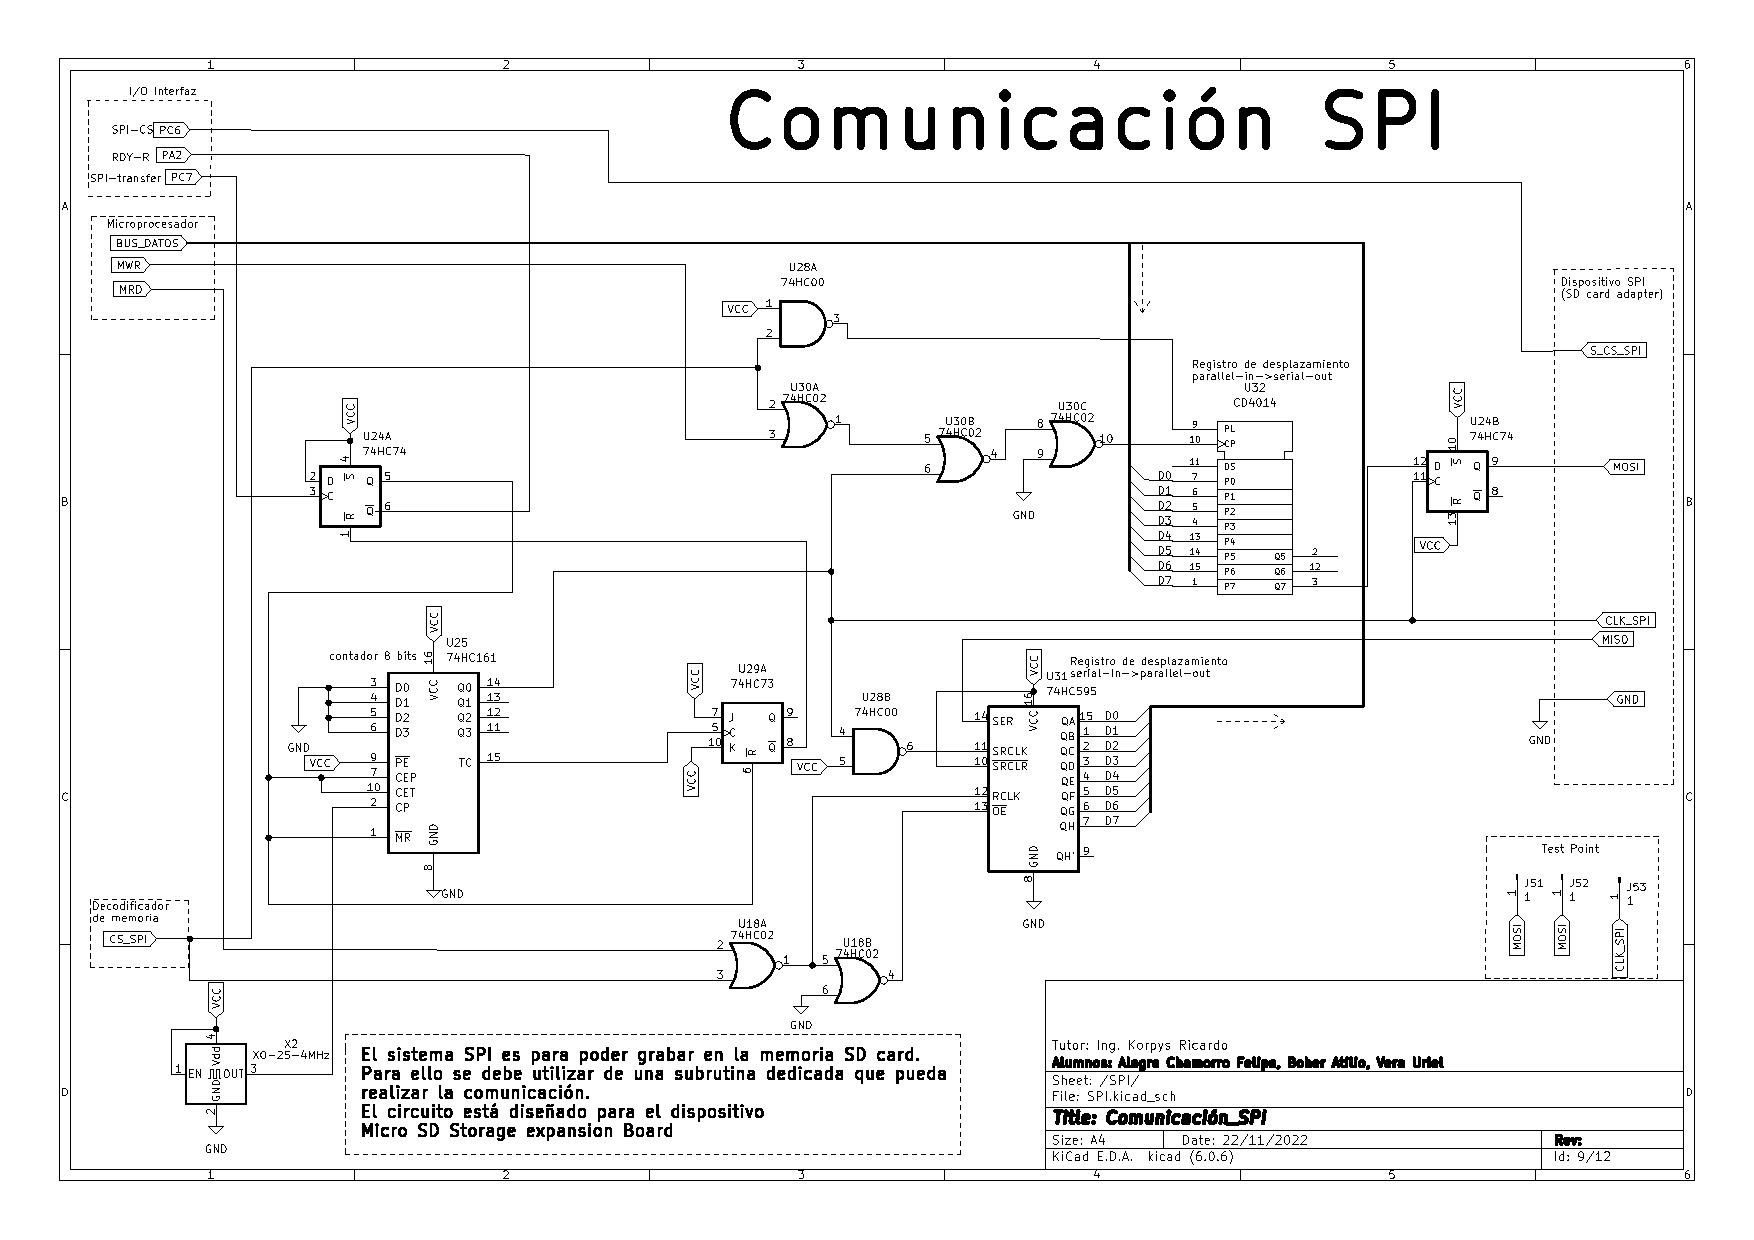
\includegraphics[width=1.2\textwidth, angle=90]{./imagenes/EsquematicosSF/Esquematico (9).pdf}
  \caption{Esquema de comunicación SPI de sistema final}
  \label{F:EsqSF9}
\end{figure}

Para el control del sistema se desarrolló un algoritmo simple el cual se presenta en el listado \ref{L:instrucciones_V3}. El funcionamiento general de este sistema se puede desglosar en tres partes. El proceso en el cual se guarda el dato a transmitir, presentado en la figura~\ref{F:DT1_SPI}; la transmisión, presentada en la figura~\ref{F:DT2_SPI}, y la lectura del dato recibido, presentada en la figura~\ref{F:DT3_SPI}. El código assembler presentado en los gráficos se corresponde con el algoritmo presentado en el listado \ref{L:instrucciones_V3}.

\begin{figure}[H]
  \centering
  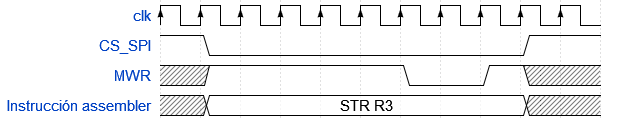
\includegraphics[width=0.55\textwidth]{./imagenes/EscrituraSPI.png}
  \caption{Proceso de guardado de dato a transmitir}
  \label{F:DT1_SPI}
\end{figure}

\begin{figure}[H]
  \centering
  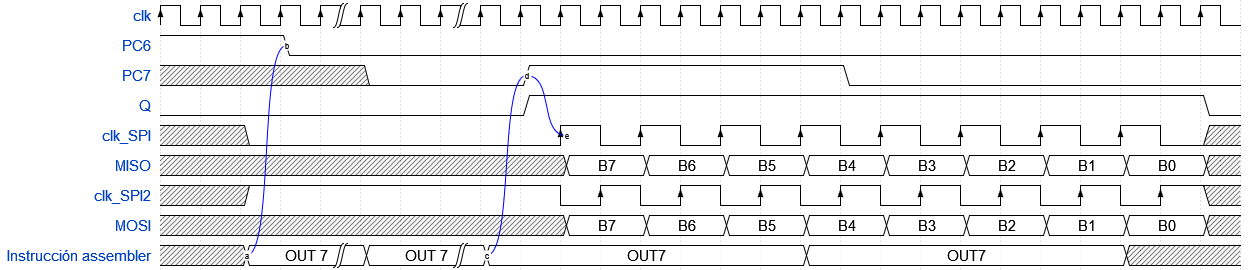
\includegraphics[width=1\textwidth]{./imagenes/TransmisionSPI.png}
  \caption{Proceso de transmisión SPI}
  \label{F:DT2_SPI}
\end{figure}

\begin{figure}[H]
  \centering
  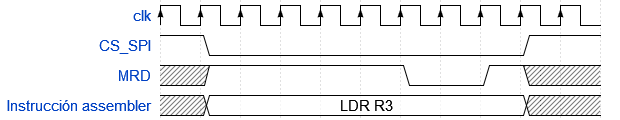
\includegraphics[width=0.55\textwidth]{./imagenes/LecturaSPI.png}
  \caption{Proceso de lectura}
  \label{F:DT3_SPI}
\end{figure}

\clearpage
\footnotesize
\lstinputlisting[language=CDP1802, caption={\centering Rutina propuesta para la transmisión utilizando el circuito de comunicación SPI}, label = {L:instrucciones_V3}]{codigo/instrucciones_V3.asm}
\normalsize

\clearpage
\subsection{Alimentación de compuertas}
La alimentación de compuertas es un esquemático en el cual se representan los puntos de alimentación de los circuitos integrados y los elementos no usados de los dispositivos electrónicos. Principalmente sirve para tener una vista más limpia en los demás esquemas.

\begin{figure}[ht]
  \centering
  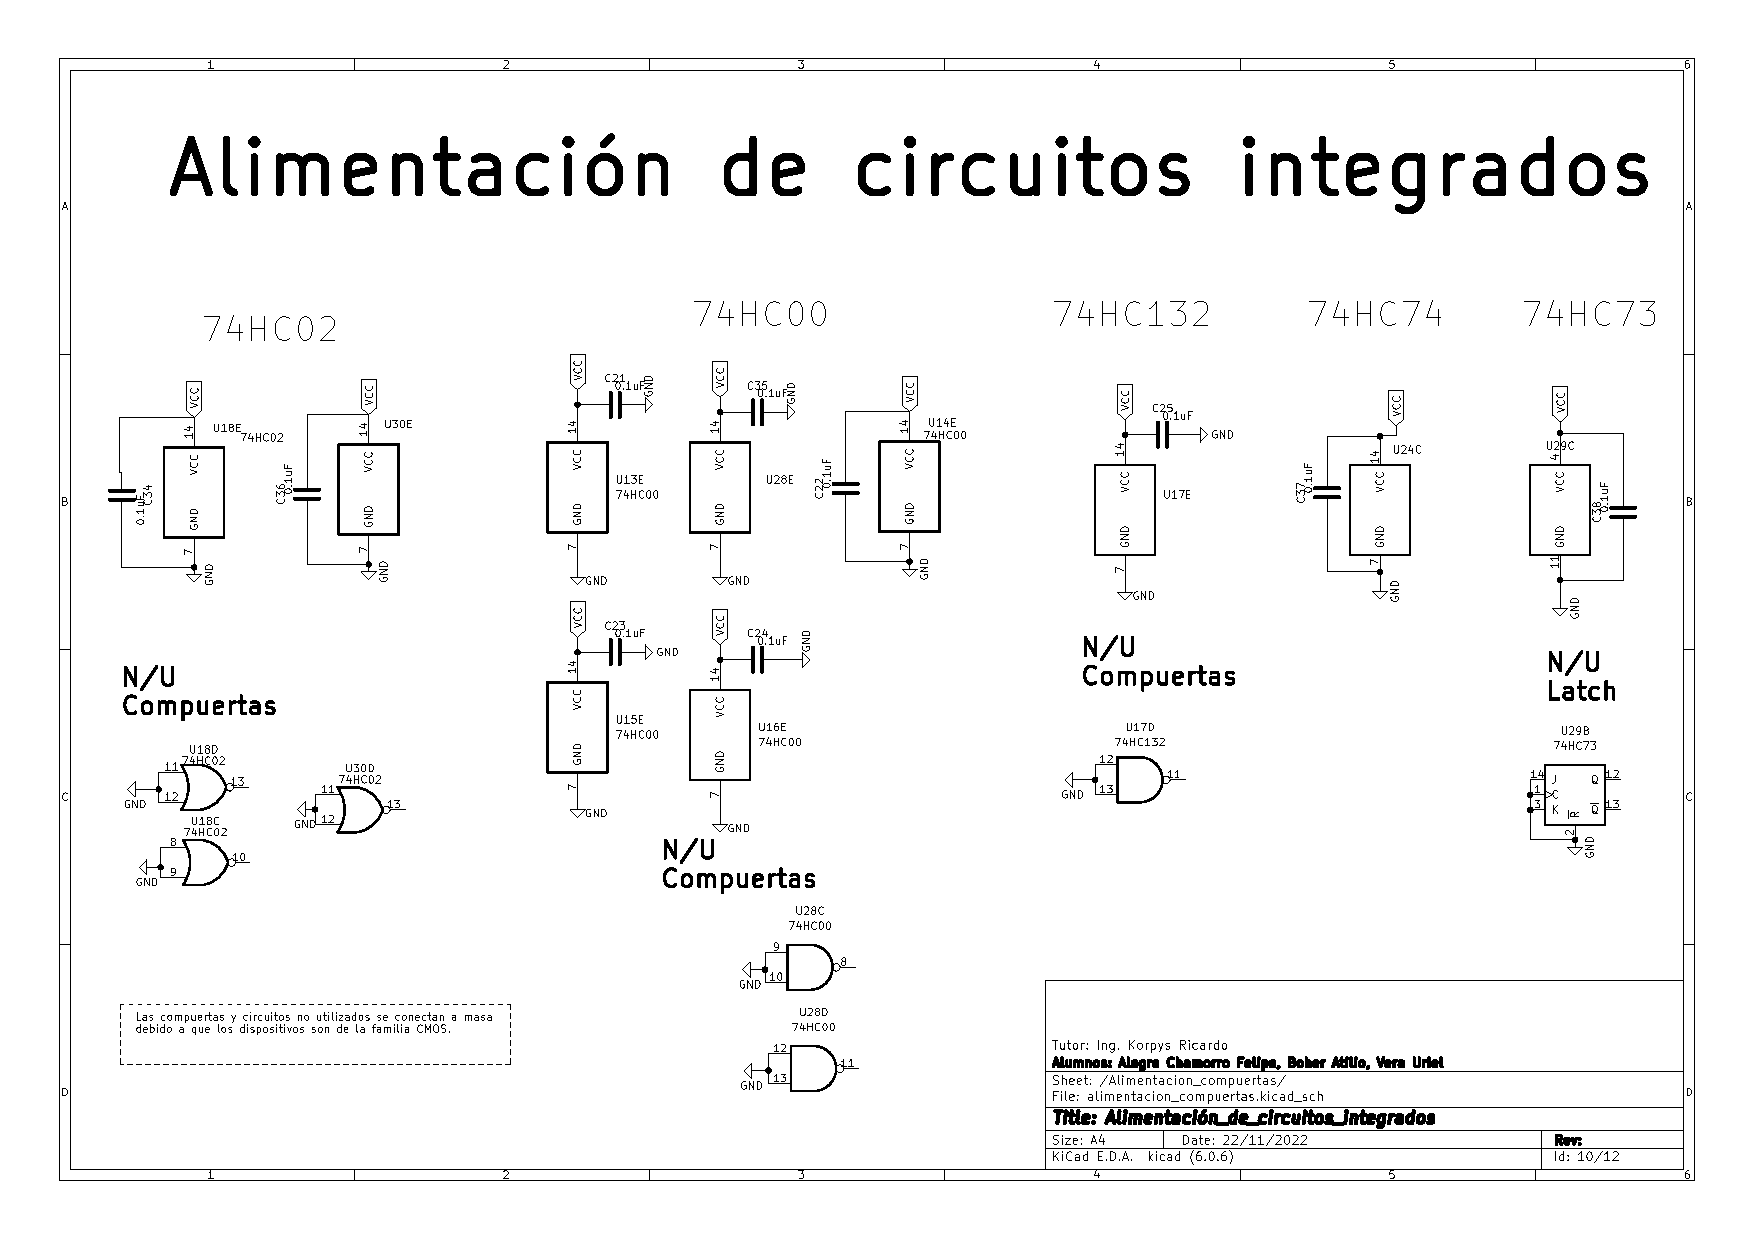
\includegraphics[width=1.2\textwidth, angle=90]{./imagenes/EsquematicosSF/Esquematico (10).pdf}
  \caption{Esquema de alimentación de compuertas de sistema final}
  \label{F:EsqSF10}
\end{figure}

\clearpage
\subsection{Interfaz I/O}
\label{C:I/O}

El microprocesador CDP1802 posee una arquitectura poco común, la cual cuenta con un mapa de memoria separado para los dispositivos de entrada y salida. Esto le da la capacidad al microprocesador de poder acceder a la memoria y a los dispositivos de entrada y salida al mismo tiempo, es decir, con la ejecución de una sola instrucción.

En el set de instrucciones~\cite{cdp1802_datasheet} puede verse la descripción de las instrucciones de entrada y salida. Por un lado, la instrucción \entreComillas{INP}, para leer datos de un dispositivo de entrada y salida:

\begin{equation*}
    \text{ BUS } \rightarrow \text{ M(R(X)) ; BUS} \rightarrow \text{ D }
\end{equation*}

Es decir, el microprocesador actúa sobre el dispositivo de entrada para que este coloque el dato a leer en el BUS de datos, luego lo almacena en la dirección de memoria apuntada por \textbf{R(X)}.

Algo similar sucede con la instrucción para enviar datos a un dispositivo, denominada \entreComillas{OUT}:

\begin{equation*}
    \text{ M(R(X)) } \rightarrow \text{ BUS ; R(X)+1} \rightarrow \text{ R(X) }
\end{equation*}

Es decir, el microprocesador coloca en el bus de datos el dato guardado en la posición de memoria apuntada por \textbf{R(X)}, y luego actúa sobre el dispositivo de salida para que este lea el dato.

Lo que significa esto es que el microprocesador no puede usar directamente sus pines \textit{Memory Write} ($ \overline{\text{MWR}} $) o \textit{Memory Read} ($ \overline{\text{MRD}} $) en un dispositivo de entrada y salida, dado que los mismos se utilizan para acceder a la memoria. Para solventar eso, el microprocesador utiliza los pines TPA, TPB y $ \overline{\text{MRD}} $, en conjunto con un circuito lógico para actuar sobre el dispositivo de entrada y salida.

Este circuito lógico se obtuvo de la figura~98 de la página~77 del manual del CDP1802~\cite{cdp1802_manual}; en conjunto con la figura~1 de la página~4 de la hoja de datos del CDP1853~\cite{datasheet_CDP1853}, resultando en el circuito de la figura~\ref{F:EsqSF11}.

\begin{figure}[ht]
  \centering
  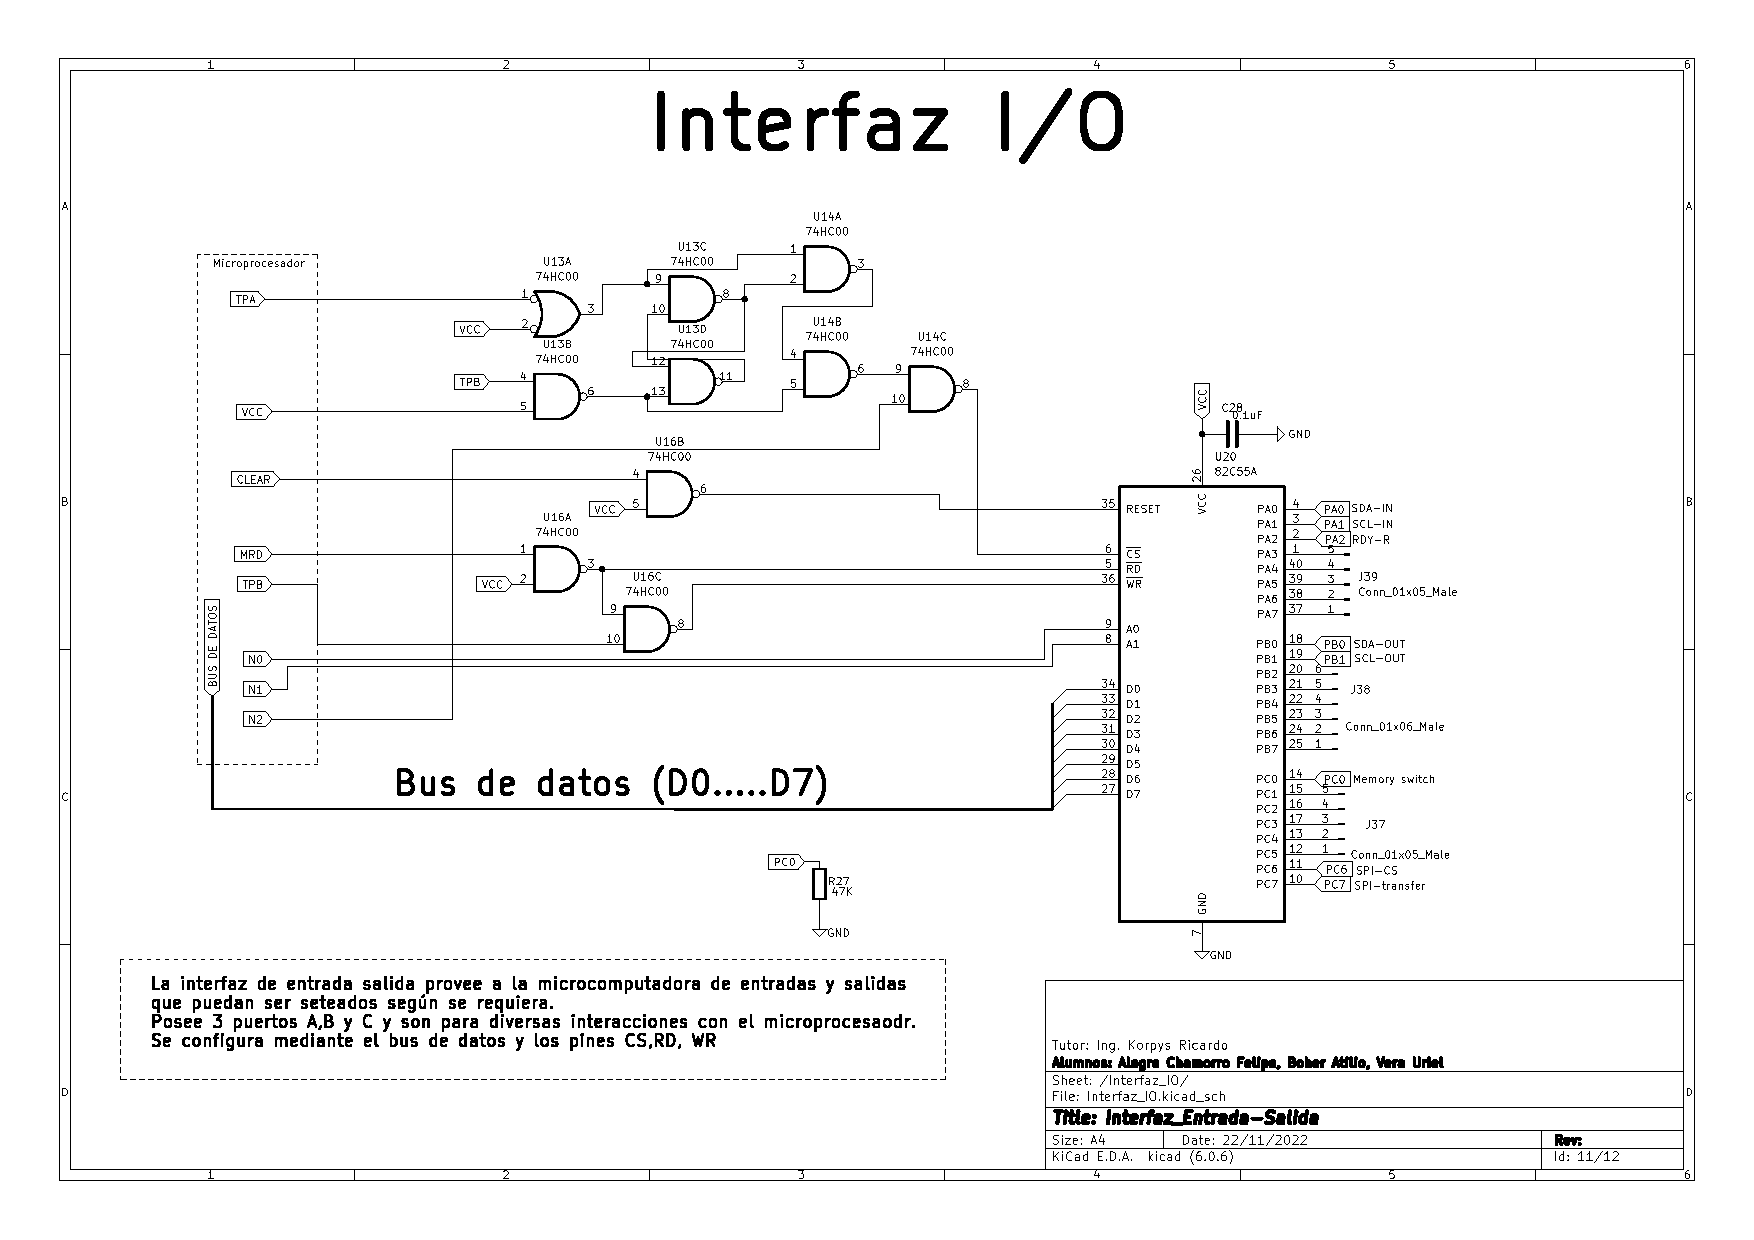
\includegraphics[width=1.2\textwidth, angle=90]{./imagenes/EsquematicosSF/Esquematico (11).pdf}
  \caption{Esquema de interfaz de entrada/salida de sistema final}
  \label{F:EsqSF11}
\end{figure}

Con este circuito es posible controlar las salidas y leer las entradas del 82C55 utilizando las instrucciones de entrada y salida del CDP1802 (INP y OUT). Todas las instrucciones utilizables se encuentran en las tablas~\ref{T:82c55_inp} y \ref{T:82c55_out}, junto a una descripción de la acción realizada por las mismas.

\begin{table}[ht!]
\caption{Instrucciones INP utilizables con el 82C55}
\label{T:82c55_inp}
\begin{tabular}{|c|c|}
\hline
Instrucción & Acción \\ \hline \hline
INP 4       & Guarda en M(R(X)) y en D el dato presente en el puerto A del 82C55     \\ \hline
INP 5       & Guarda en M(R(X)) y en D el dato presente en el puerto B del 82C55    \\ \hline
INP 6       & Guarda en M(R(X)) y en D el dato presente en el puerto C del 82C55    \\ \hline
INP 7       & Guarda en M(R(X)) y en D el dato presente en el registro de control del 82C55     \\ \hline
\end{tabular}
\end{table}

\begin{table}[ht!]
\caption{Instrucciones OUT utilizables con el 82C55}
\label{T:82c55_out}
\begin{tabular}{|c|c|}
\hline
Instrucción & Acción \\ \hline \hline
OUT 4       & Escribe el dato M(R(X)) en el puerto A del 82C55     \\ \hline
OUT 5       & Escribe el dato M(R(X)) en el puerto B del 82C55     \\ \hline
OUT 6       & Escribe el dato M(R(X)) en el puerto C del 82C55     \\ \hline
OUT 7       & Escribe el dato M(R(X)) en el registro de control del 82C55     \\ \hline
\end{tabular}
\end{table}

\clearpage
\subsection{BUS I2C}
\label{C:BUSI2C}

El esquema presentado para el bus I2C presenta una interfaz construida a partir de transistores NPN. La razón de esta interfaz radica en la característica de los dispositivos I2C, que se conectan al bus mediante una interfaz de drenador abierto. Esto podría generar cortocircuitos en un accionamiento simultáneo del bus, por lo que se requiere de esta interfaz.

\begin{figure}[ht]
  \centering
  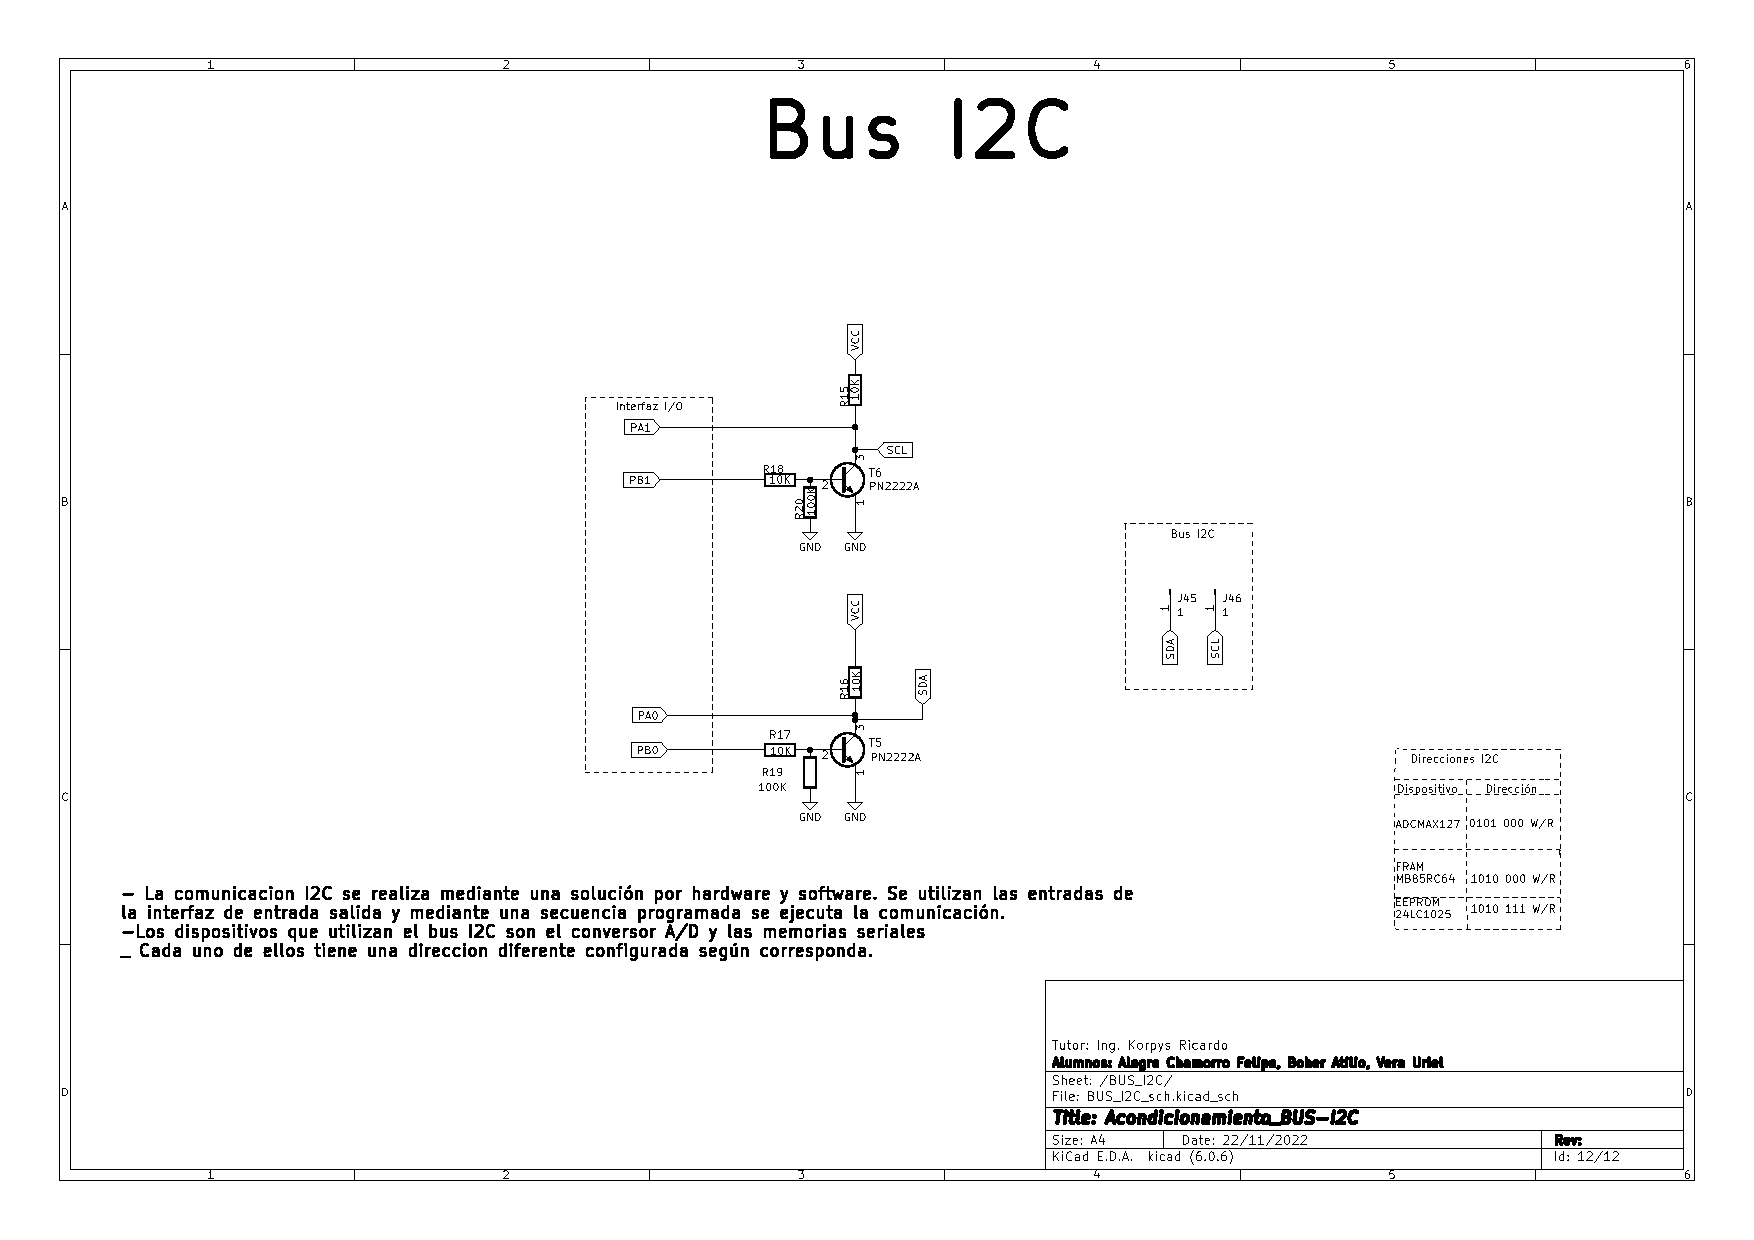
\includegraphics[width=1.2\textwidth, angle=90]{./imagenes/EsquematicosSF/Esquematico (12).pdf}
  \caption{Esquema de bus I2C de sistema final}
  \label{F:EsqSF12}
\end{figure}

\clearpage
\section{Lista de componentes}

En la tabla~\ref{T:bom_sis_final} se encuentra la lista de materiales para la construcción del sistema final.

\footnotesize
\begin{longtable}{|p{0.08\textwidth}|p{0.11\textwidth}|p{0.30\textwidth}|p{0.14\textwidth}|p{0.15\textwidth}|}
\caption{Lista de componentes del sistema final} % needs to go inside longtable environment
\label{T:bom_sis_final}
\\
\hline
Cantidad & Etiqueta \newline
           Identificador            & Descripción                               & Fabricante            & Número de parte       \\ \hline \hline \endfirsthead
\hline
Cantidad & Etiqueta \newline
           Identificador            & Descripción                               & Fabricante            & Número de parte       \\ \hline \hline \endhead
1       & U1                        & Microprocesador                           & RCA                   & CDP1802ACE            \\ \hline
1       & U2                        & Latch de 8 bits                           & Philips               & 74HC573N              \\ \hline
1       & U3                        & Memoria EEPROM 32k x 8                    & XICOR                 & X28C256D-25           \\ \hline
1       & U4                        & Memoria EEPROM Serial I2C 128k x 8        & Microchip             & 24LC1025              \\ \hline
1       & U5                        & Time keeping RAM 32K x8                   & Dallas                & DS1744-070            \\ \hline
1       & U6                        & Memoria RAM 32k x 8                       & HYUNDAI               & HY62256ALP-10         \\ \hline
1       & U7                        & Memoria FRAM Serial I2C 8k x 8            & Fujitsu Semiconductor & MB85RC64A            \\ \hline
1       & U8                        & Conversor analógico-digital con interfaz I2C & Maxim Integrated   & MAX127                \\ \hline
1       & U9                        & Regulador de tensión 12~\si{\volt}        & Motorola              & 7812CT                \\ \hline
1       & U10                       & Regulador de tensión 5~\si{\volt}         & ST Microelectronics   & L7805CV               \\ \hline
1       & U11                       & High Precision Operational Amplifier      & Burr-Brown            & OPA4277PA             \\ \hline
1       & U12                       & Regulador de tensión -12~\si{\volt}       & ST Microelectronics   & L7912CV               \\ \hline
5       & U13, U14, U15, U16, U28   & Cuádruple compuerta NAND de dos entradas  & Texas Instruments     & SN74HC00N             \\ \hline
1       & U17                       & Cuádruple compuerta NAND de dos entradas con Schmitt-Trigger & Texas Instruments& SN74HC132N \\ \hline
2       & U18,U30                   & Cuádruple compuerta NOR de dos entradas   & Texas Instruments     & SN74HC02N             \\ \hline
1       & U19                       & Decodificador Multiplexador 3 a 8 líneas  & Texas Instruments     & SN74HC138N            \\ \hline
1       & U20                       & CMOS Programmable Peripheral Interface    & Intersil              & CP82C55A-5Z           \\ \hline
1       & U21                       & Regulador programable shunt               & Fairchild             & LM336Z25              \\ \hline
1       & U24                       & Doble flip-flop tipo D con Set y Reset    & Texas Instruments     & SN74HC74N             \\ \hline
1       & U25                       & Contador binario de 4 bits                & Fairchild Semiconductor & MM74HC161N          \\ \hline
1       & U29                       & Doble flip-flop JK con Set y Reset        & National Semiconductor & MM74HC73N           \\ \hline
1       & U31                       & Registro de desplazamiento de 8 bits      & Texas Instruments     & SN74HC595N            \\ \hline
1       & U32                       & Registro de desplazamiento de 8 estados   & Motorola              & MC14014BCP            \\ \hline
1       & X2                        & XO-22BE-4MHz                              &   \listaVacio                    & \listaVacio                      \\ \hline
1       & XTAL1                     & Cristal \num{4}~\si{\mega\hertz}          & CQ Electronics        & \listaVacio                      \\ \hline
1       & SW1                       & Llave DPDT 6 pines                        & \listaVacio                      & \listaVacio                      \\ \hline
3       & SW2, SW3, SW4             & Pulsador 6mm~x~4,3mm                      &  \listaVacio                     &  \listaVacio                     \\ \hline
5       & T2, T3, T4, T5, T6        & Transistor BJT NPN                        & Motorola              & P2N2222A               \\ \hline
1       & RV1                       & Preset 10~\si{\kilo\ohm}                  &  \listaVacio                     &  \listaVacio                     \\ \hline
1       & D1                        & Puente rectificador de onda completa B380R &            \listaVacio           &  \listaVacio                     \\ \hline
6       & D2, D3, D4, D5, D6, D7    & LED 5~mm                                  &\listaVacio                       &   \listaVacio                    \\ \hline
2       & D8, D9                    & 1N914                                     &\listaVacio                       &  \listaVacio                     \\ \hline
1       & F1                        & Fusible 10~mm 1~\si{\ampere}              &\listaVacio                       &  \listaVacio                     \\ \hline
8       & R1, R2, R3, R5, R21, R22, R23, R27
                                    & Resistor 47~\si{\kilo\ohm} 1/8~\si{\watt} & \listaVacio                      &   \listaVacio                    \\ \hline
1       & R4                        & Resistor 10~\si{\mega\ohm} 1/8~\si{\watt} &  \listaVacio                     &   \listaVacio                    \\ \hline
1       & R6                        & Resistor 330~\si{\ohm} 1/4~\si{\watt}     &  \listaVacio                     &   \listaVacio                    \\ \hline
2       & R7, R8                    & Resistor 1~\si{\kilo\ohm} 1/8~\si{\watt}  &  \listaVacio                     &    \listaVacio                   \\ \hline
3       & R9, R10, R11              & Resistor 220~\si{\ohm} 1/4~\si{\watt}     &    \listaVacio                   &    \listaVacio                   \\ \hline
16      & R12, R13, R14, R15, R16, R17, R18, R38, R39, R40, R41, R46, R47, R56, R57, R60
                                    & Resistor 10~\si{\kilo\ohm} 1/8~\si{\watt} & \listaVacio                      &   \listaVacio                    \\ \hline
5       & R19, R20, R24, R25, R26   & Resistor 100~\si{\kilo\ohm} 1/8~\si{\watt}&  \listaVacio                     &   \listaVacio                    \\ \hline
4       & R28, R30, R36, R52        & Resistor 100~\si{\ohm} 1/4~\si{\watt}     &  \listaVacio                     &   \listaVacio                    \\ \hline
4       & R29, R31, R37, R53        & Resistor 150~\si{\ohm} 1/4~\si{\watt}     &  \listaVacio                     &   \listaVacio                    \\ \hline
8       & R32, R33, R34, R35, R42, R43, R54, R55
                                    & Resistor 390~\si{\kilo\ohm} 1/8~\si{\watt}&  \listaVacio                     & \listaVacio                      \\ \hline
8       & R44, R45, R48, R49, R50, R51, R58, R59
                                    & Resistor 1~\si{\mega\ohm} 1/8~\si{\watt}  &  \listaVacio                     & \listaVacio                      \\ \hline
2       & C2, C3                    & Capacitor cerámico \num{30}~\si{\pico\farad} 50~\si{\volt}
                                                                                &   \listaVacio                    & \listaVacio                      \\ \hline
14       & C5, C7, C8, C29, C30, C31, C14, C15, C18, C32, C33, C39, C40, C43
                                    & Capacitor cerámico \num{0.10}~\si{\micro\farad} 50~\si{\volt}
                                                                                &    \listaVacio                   &   \listaVacio                    \\ \hline
2       & C11, C17                  & Capacitor electrolítico 4700~\si{\micro\farad} 25~\si{\volt}
                                                                                &     \listaVacio                  &   \listaVacio                    \\ \hline
2       & C12, C16                  & Capacitor cerámico \num{0.33}~\si{\micro\farad} 50~\si{\volt}
                                                                                &   \listaVacio                    &  \listaVacio                     \\ \hline
1       & C13                       & Capacitor electrolítico 10~\si{\micro\farad} 25~\si{\volt}
                                                                                &   \listaVacio                    &  \listaVacio                     \\ \hline
1       & C19                       & Capacitor electrolítico \num{0.01}~\si{\micro\farad} 25~\si{\volt}
                                                                                &     \listaVacio                  &  \listaVacio                     \\ \hline
1       & C20                       & Capacitor electrolítico \num{4.7}~\si{\micro\farad} 25~\si{\volt}
                                                                                &   \listaVacio                    &  \listaVacio                     \\ \hline
6       & J1, J2, J33, J48, J49, J50& 1x3 Pines Conectores Macho \num{2.54}~mm  &   \listaVacio                    &  \listaVacio                     \\ \hline
38      & J3, J4, J5, J6, J7, J8, J9, J10, J11, J12, J13, J14, J15, J16, J17, J18, J19, J20, J21, J22, J23, J24, J25, J26, J27, J28, J29, J30, J31, J36, J40, J41, J42, J45, J46, J51, J52, J53
                                    & Pin conector macho (1 \textit{Male Header Pin}) & \listaVacio                      &   \listaVacio                    \\ \hline
3       & J32, J35, J38             & 1x6 Pines Conectores Macho \num{2.54}~mm  & \listaVacio                      & \listaVacio                      \\ \hline
3       & J34, J37, J39             & 1x5 Pines Conectores Macho \num{2.54}~mm  & \listaVacio                      &   \listaVacio                    \\ \hline
2       & J43, J44                  & Bornera 3 pines \num{5.08}~mm             &  \listaVacio                     &  \listaVacio                     \\ \hline
2       & J47, J54                  & 1x12 Pines Conectores Macho \num{2.54}~mm &   \listaVacio                    &  \listaVacio                     \\ \hline
1       & J55                       & 1x2 Pines Conectores Macho \num{2.54}~mm  &   \listaVacio                    &   \listaVacio                    \\ \hline
1       & No aplica                 & Módulo conversor USB-Serial               & Future Technology Devices International & FT232RL \\ \hline
1       & No aplica                 & Módulo adaptador tarjeta micro SD         & \listaVacio  & \listaVacio \\ \hline
\end{longtable}
\normalsize

\section{Placa PCB}
La placa PCB fue desarrollada en KiCad, al igual que los anteriormente mencionados. En la misma se incluyen todas las partes presentadas en los esquemáticos de la sección \ref{C:EsqSF}. Para ello se requirió un tamaño de 30~cm de largo por 30~cm de ancho, en una placa doble faz. Ambos lados y la máscara de componentes se presentan en las figuras \ref{F:PCB_frente}, \ref{F:PCB_atras} y \ref{F:PCB_mascara}. Sin embargo, se adjuntarán en tamaño original en el apéndice. 
Por otro lado, se presenta una visión en tres dimensiones creada por el mismo software de diseño en la figura~\ref{F:PCB_3D}.


\begin{figure}[H]
  \centering
  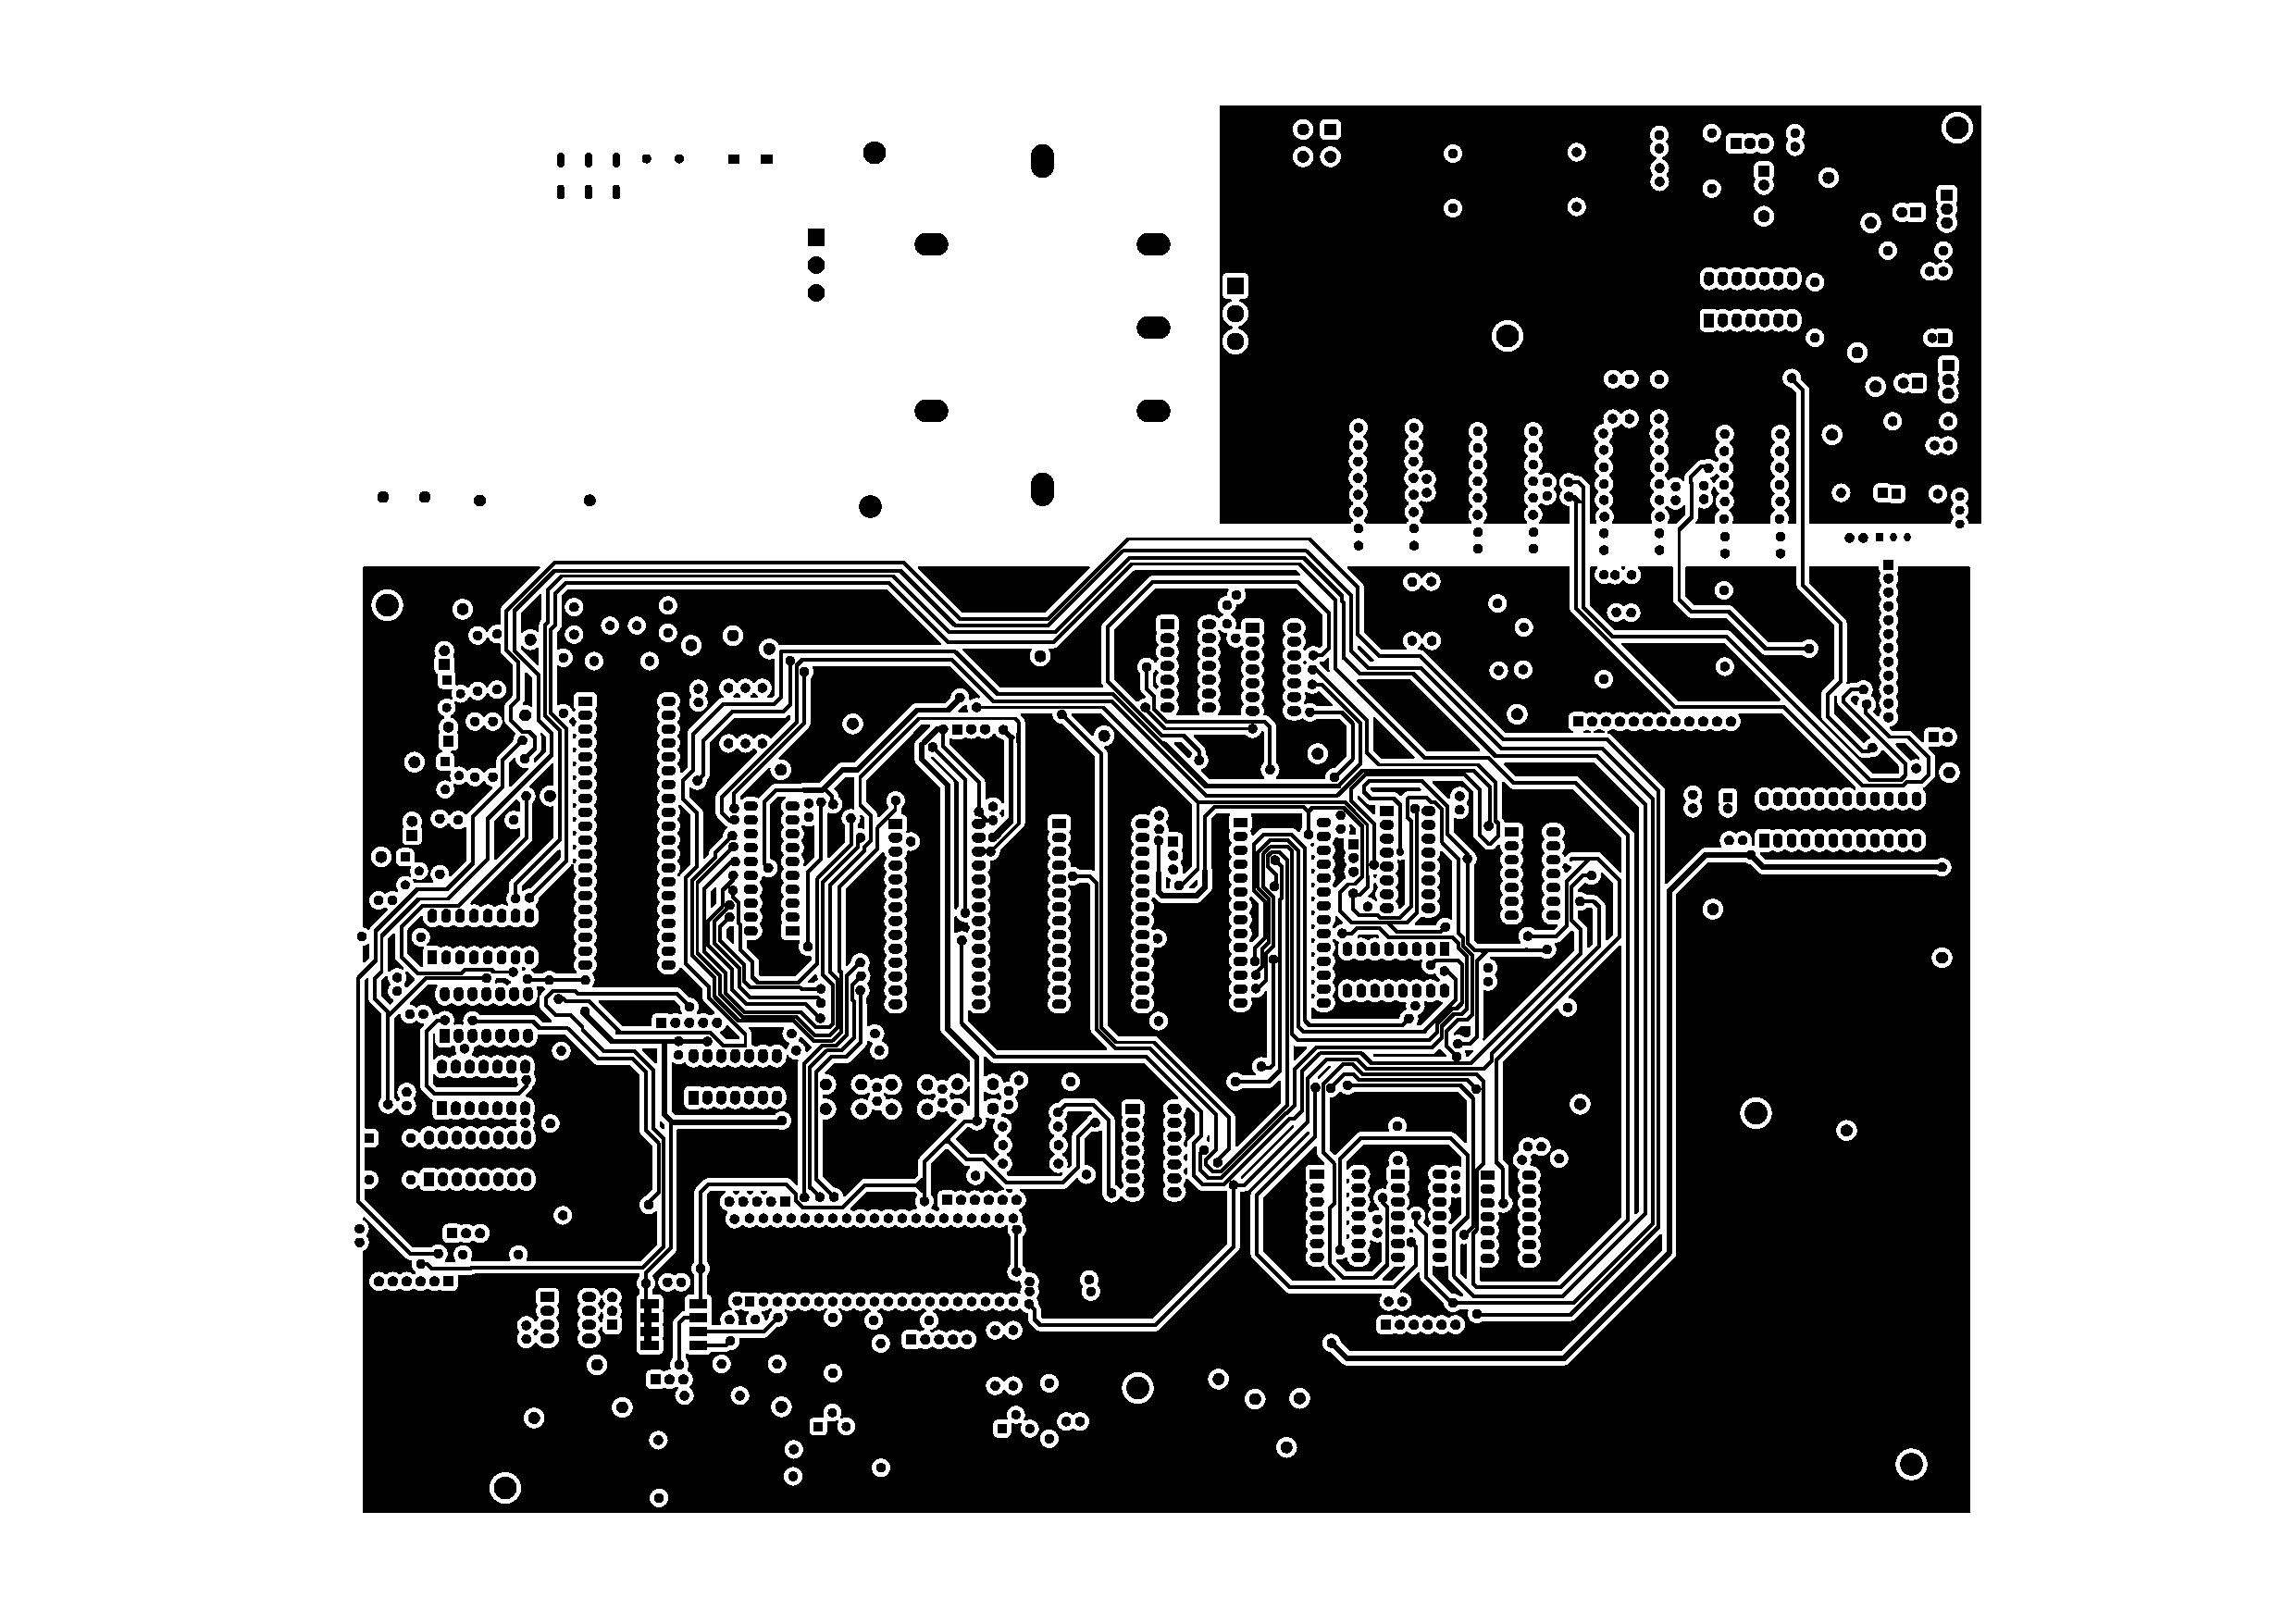
\includegraphics[width=1\textwidth]{./imagenes/EsquematicosSF/PCB_frente.pdf}
  \caption{Pistas de PCB sistema final parte frontal}
  \label{F:PCB_frente}
\end{figure}

\begin{figure}[H]
  \centering
  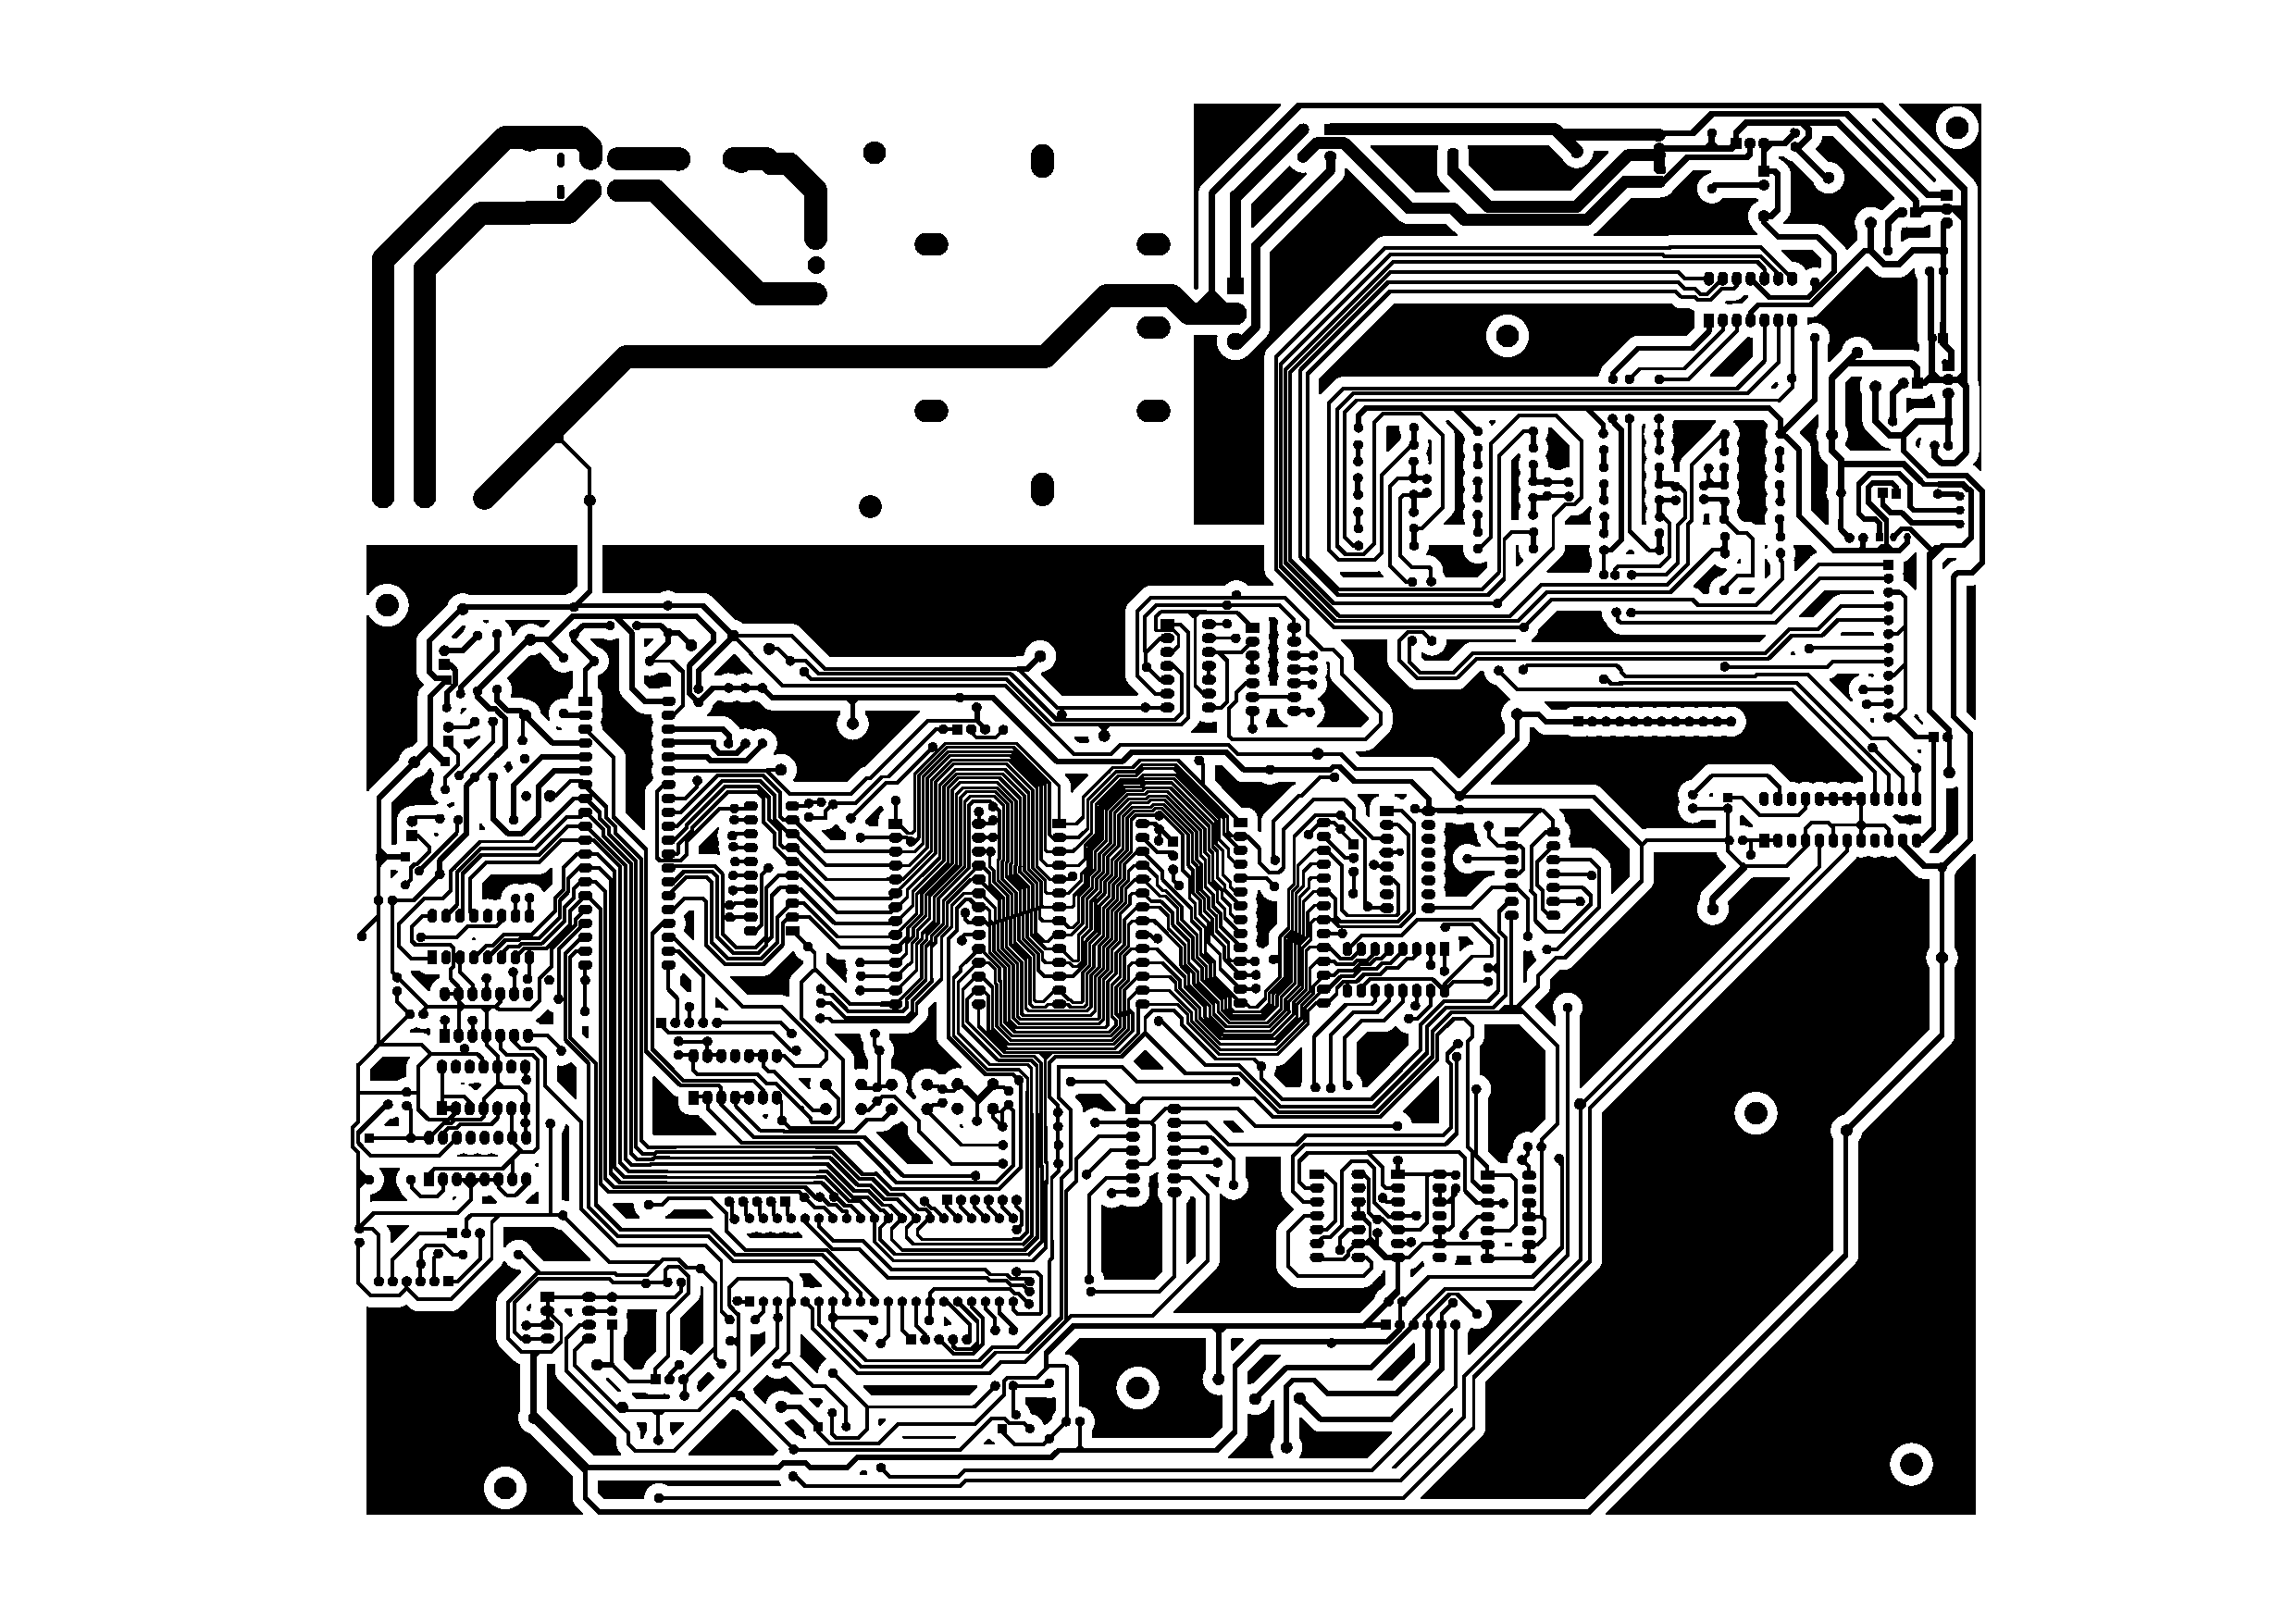
\includegraphics[width=1\textwidth]{./imagenes/EsquematicosSF/PCB_atras.pdf}
  \caption{Pistas de PCB sistema final parte posterior}
  \label{F:PCB_atras}
\end{figure}

\begin{figure}[H]
  \centering
  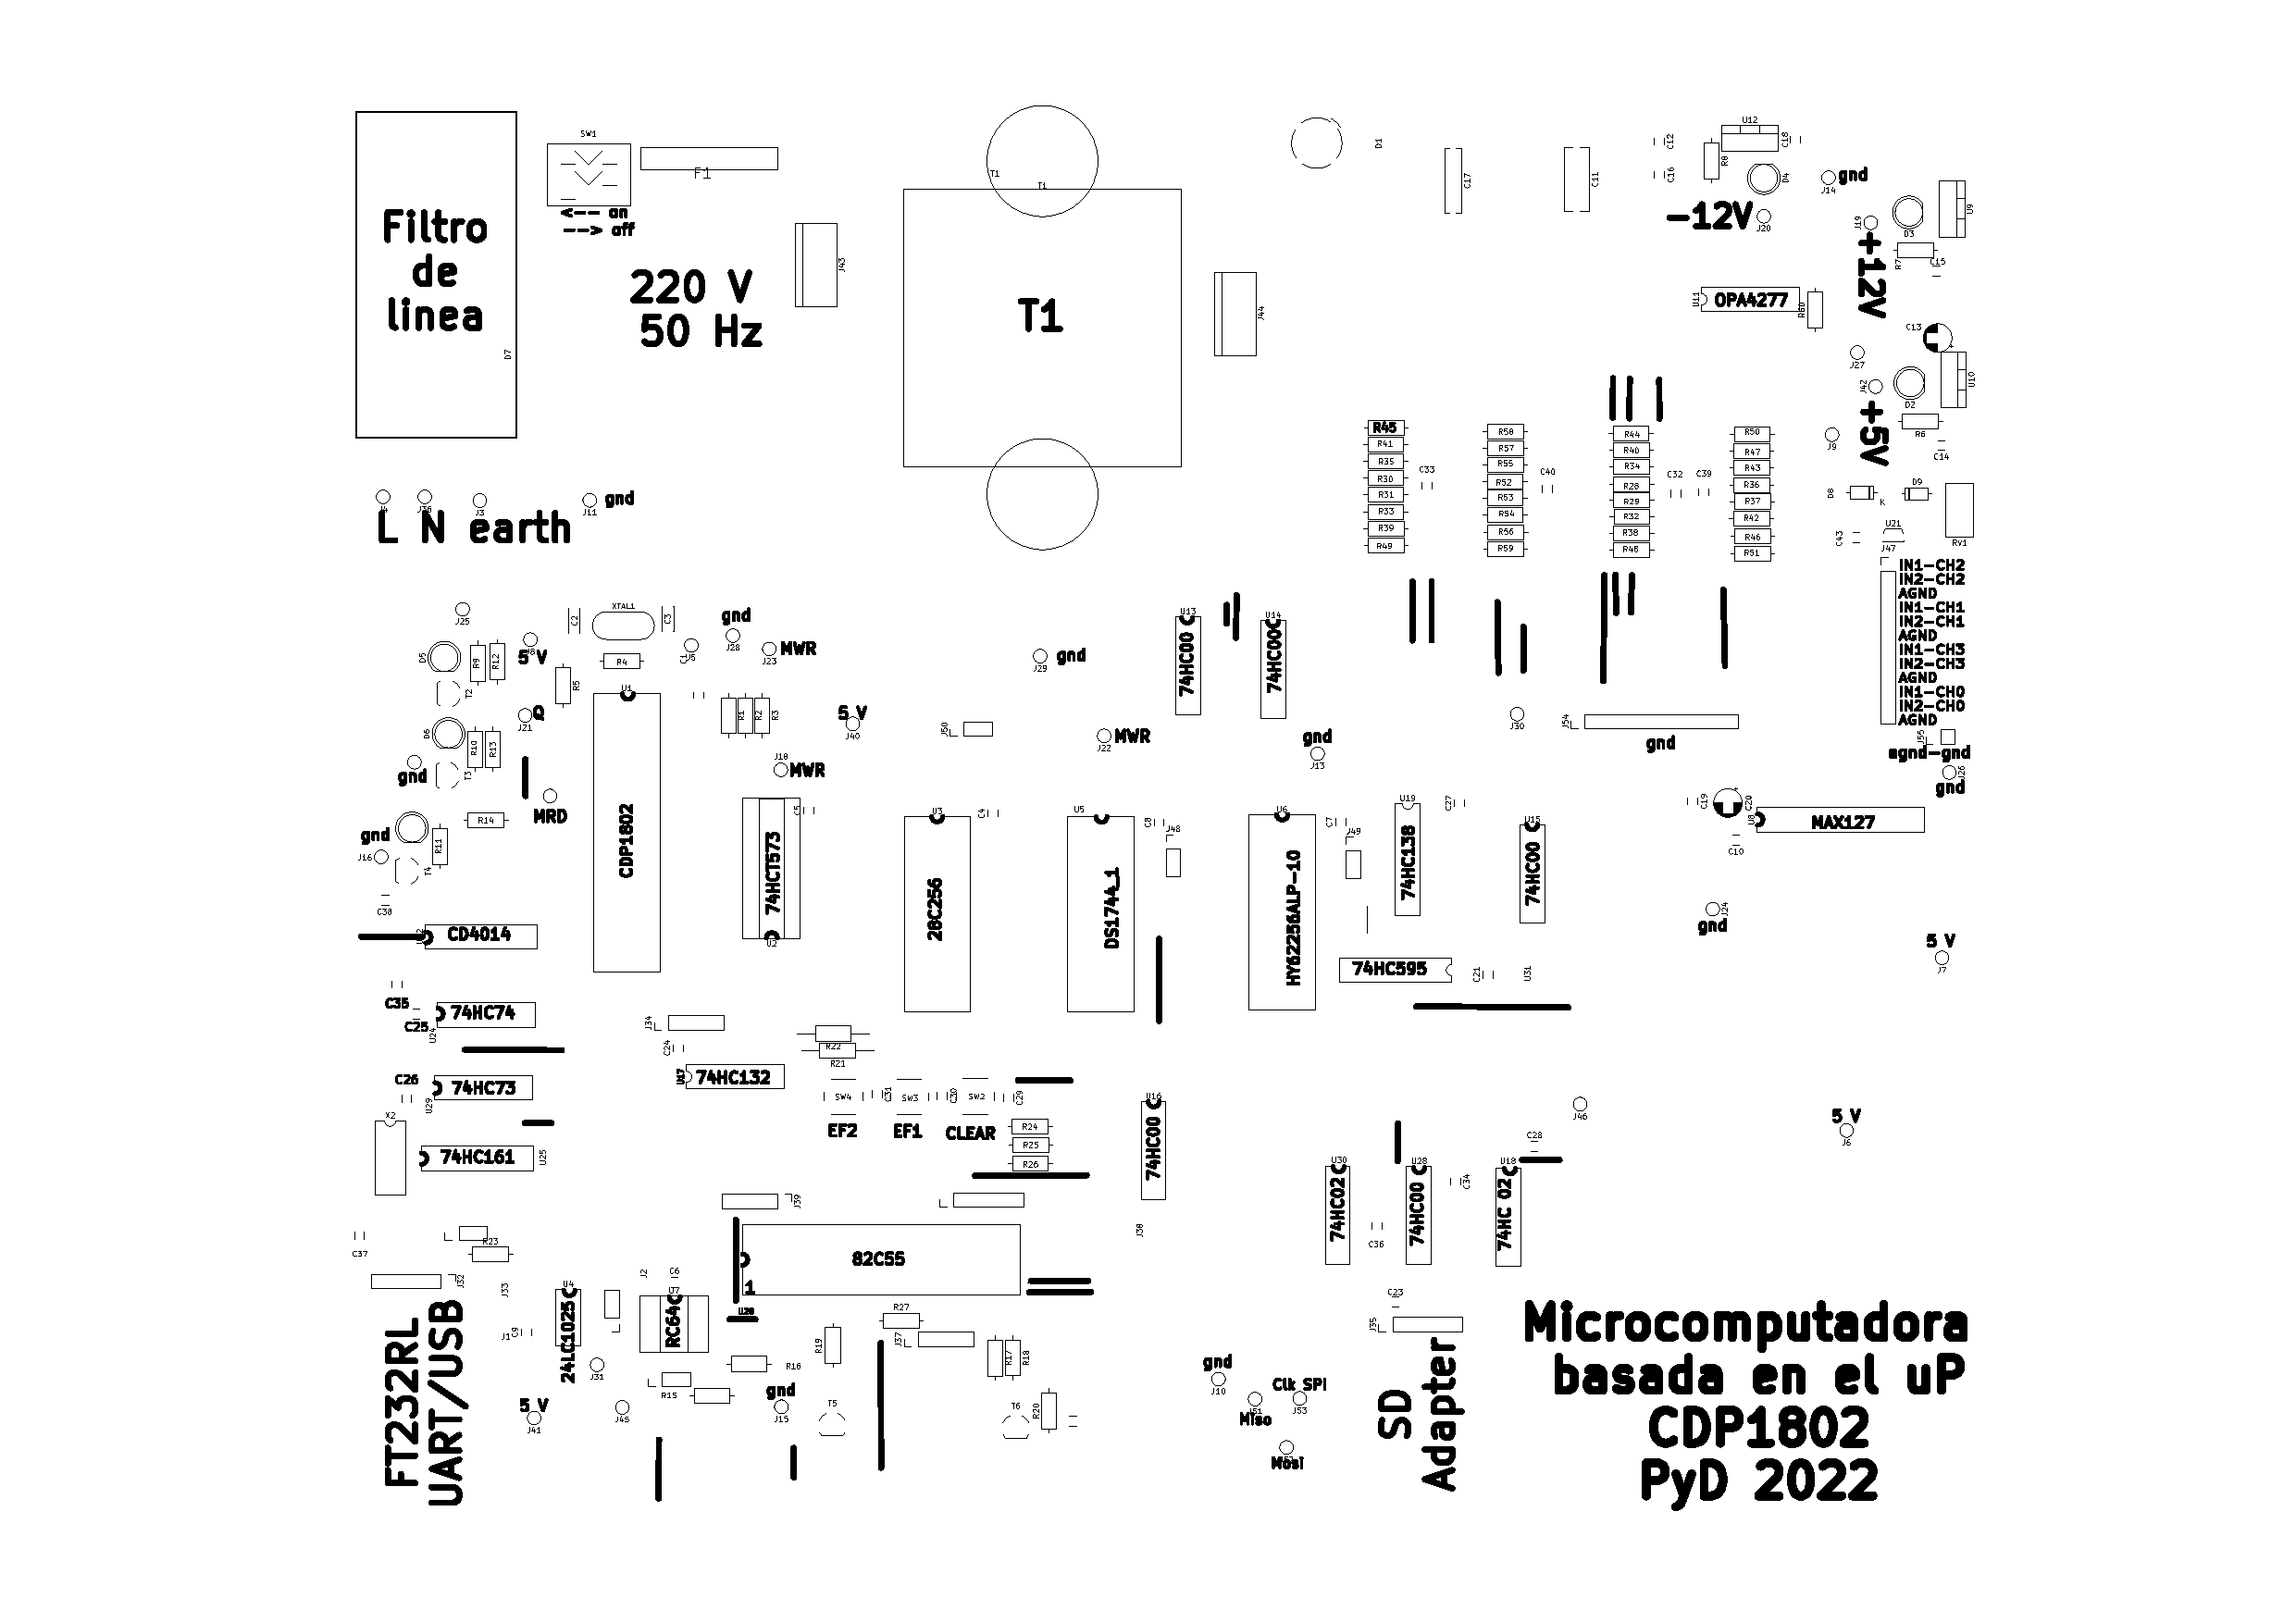
\includegraphics[width=1\textwidth]{./imagenes/EsquematicosSF/PCB_mascara.pdf}
  \caption{Máscara de componentes de PCB de sistema final}
  \label{F:PCB_mascara}
\end{figure}

\begin{figure}[H]
  \centering
  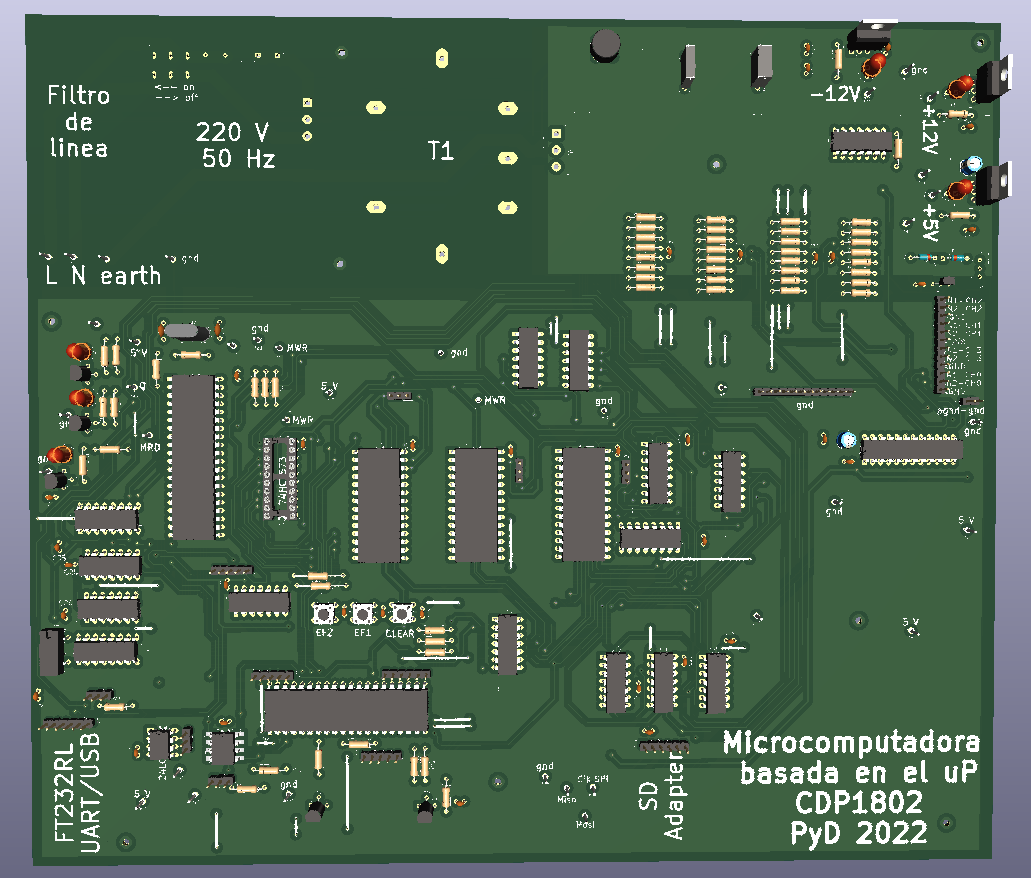
\includegraphics[width=1\textwidth]{./imagenes/sistema_final_3D.png}
  \caption{Visión en tres dimensiones de sistema final}
  \label{F:PCB_3D}
\end{figure}


% ----------------------------------------
 \chapter{Conclusiones}
% ----------------------------------------
\label{C:conclusiones}

Se han estudiado las características correspondientes al microprocesador CDP1802 y entendido el principio de funcionamiento del mismo, conocimiento que fue aplicado para el desarrollo de diferentes circuitos de complejidad progresiva que se encuentran explicados en el presente documento. Se han reconocido los fundamentos y funcionalidades de los elementos correspondientes a una microcomputadora, como ser memorias, interfaz de entrada salida, conversor analógico digital, entre otras, de tal manera de poder proyectar subsistemas dedicados a funciones específicas que tengan interoperabilidad entre los mismos, seleccionando los diferentes dispositivos adecuadamente para su compatibilidad en las diferentes aplicaciones. Se analizaron circuitos y placas de desarrollo con el microprocesador utilizado, que sirvieron de base para los sistemas proyectados en este trabajo. 

Se han desarrollado competencias en el análisis de costos, pedidos de presupuesto y toda la logística involucrada en el proyecto e implementación de un circuito electrónico, comprendiendo las utilidades presentadas por un proceso de planificación y administración del tiempo, como el diagrama de Gantt, y también se ganó experiencia con herramientas de redacción de informes que permiten plasmar los resultados obtenidos en cualquier ámbito de manera profesional. 

Se han estudiado, analizado, comprendido y simulado diferentes arquitecturas que utilizan el microprocesador CDP1802, cuyos resultados brindaron entendimiento respecto a las topologías propuestas. Se utilizaron herramientas de simulación (Emma02, Proteus) que presentan herramientas de depuración, las cuales fueron sumamente importantes para detectar errores que presentan complejidad para detectarse en el circuito físico y corroborar el funcionamiento de las placas de desarrollo ya existentes con arquitecturas similares a las implementadas.

Se han proyectado, diseñado e implementado dos microcomputadoras (sistema mínimo y sistema medio) con arquitecturas diferentes y se ha logrado su correcto funcionamiento al ser probadas y testeadas. Simples programas se han implementado en el sistema mínimo y en el sistema medio, corroborando el correcto funcionamiento de los mismos. En el sistema medio se han ejecutado un intérprete de un lenguaje de programación y un sistema operativo sin disco, y se ha comprobado su correcto funcionamiento. Se ha proyectado y diseñado una microcomputadora (sistema final) que posea todas las aplicaciones planteadas desde un principio, como ser el conversor analógico digital y el uso de memorias seriales, por nombrar algunas. Se diseñaron el esquemático y el PCB del sistema final los cuales se encuentran presentes en el documento. Se logró integrar todas las funcionalidades pensadas en un principio y plasmarlas sobre el esquemático del sistema. 

Durante el desarrollo del trabajo se han utilizado y aplicado con éxito gran parte de los conocimientos obtenidos en la carrera de ingeniería electrónica y se adquirieron otros relacionados con llevar a la práctica los conceptos teóricos ya estudiados. Uno de ellos es el uso de software de diseño KiCad, en el cual se desarrollaron todos los circuitos planteados para el trabajo y la construcción de placas PCB de doble faz, entre otros. 


Como conclusión en vista de las facultades adquiridas con el desarrollo del presente trabajo, se destaca la interdependencia de software-hardware, sobre todo cuando el desarrollo de software es en bajo nivel como en este caso. Es de carácter fundamental para los diseñadores de este tipo de circuitos conocer el funcionamiento claro, uno del otro, para poder realizar un avance significativo en el desarrollo del proyecto. 

Las principales dificultades en el desarrollo del trabajo se relacionan con el entendimiento del microprocesador, el cual presenta una arquitectura particular. Se destaca principalmente el modo en el que opera con las instrucciones de entrada-salida, sin embargo, el uso de registros y su programación difieren mucho de las arquitecturas estudiadas en la carrera. 

Se han cumplimentado en gran medida los objetivos planteados para este proyecto en un principio, logrando integrar los conceptos estudiados a lo largo de la carrera correctamente y diseñar e implementar diferentes sistemas de microcómputo que sirven para sus determinadas aplicaciones. Los alumnos a cargo del proyecto han adquirido herramientas específicas para la integración de conceptos, proyecto y diseño de sistemas integrados, comprensión cabal del funcionamiento de diversos dispositivos, entre las más importantes. Estas herramientas, adquiridas por los alumnos para su próxima inserción laboral, cumplimentan así los objetivos de la materia Proyecto y Diseño Electrónico. 
\chapter{Trabajos a futuro}
\label{C:trabajos_a_futuro}

En este capítulo presentaremos una lista de actividades que pueden ser desarrolladas a partir de las bases presentadas en este trabajo. Las actividades propuestas buscan ser alcanzables con un nivel medio de dificultad considerándose como punto de partida las herramientas teórico-prácticas presentadas.

\section{Construcción de sistema final}
Se considera que el primer paso lógico a seguir, luego de lo presentado, es la construcción del sistema final. La construcción del circuito puede proveer información útil, verificando los esquemas planteados o identificando fallas del mismo. En dicha construcción se deben realizar pruebas de alimentación, comunicación entre circuitos integrados, coordinación en instrucciones simples, entre otras pruebas.


\section{Programas de prueba}
Una vez construido el sistema final, este puede ser puesto a prueba con los programas diseñados para el sistema medio y mínimo, sin embargo, estos no explotarían el potencial del circuito presentado en el sistema final. Es por ello que se requiere el diseño de programas de prueba que en principio serán simples para verificar el funcionamiento del circuito y luego podrán ser modificados para realizar tareas más complejas. 

\subsection{Coordinación de interfaz entrada-salida}
El esquema presentado en la figura~\ref{F:EsqSF11} presenta una interfaz de entrada-salida basada en el circuito integrado 82C55. Para el correcto funcionamiento de la interfaz, se debe diseñar un software capaz de controlar los puertos disponibles en el chip. Este software debería ser uno de los primeros en probarse en el sistema final, ya que sirve para comunicarse con gran parte del resto del circuito. 

\subsection{Comunicación I2C}
El circuito final cuenta con circuitos integrados que funcionan a través de la comunicación I2C. Para lograr un funcionamiento óptimo del circuito, es indispensable el planteamiento de un software que permita enviar y recibir instrucciones a estos integrados. 

\subsection{Conversión Analógico-Digital}
Una vez diseñado el sistema de comunicación I2C, se puede plantear un software que permita controlar el sistema de conversión A/D. Para ello debe poder realizar la configuración de los niveles de tensión asociados a la lectura de cada uno de los canales disponibles, así como también realizar la lectura de un canal deseado. 

\subsection{Rutina de cambio en el mapa de memoria}
Para desbloquear un mayor potencial en el funcionamiento del sistema final, se debe plantear un programa de booteo que permita transmitir la memoria de programa a la memoria RAM y luego realice el cambio en el mapa de memoria poniendo en la parte baja del mismo (0000h a 7FFFh) otra memoria RAM, permitiendo almacenar mayor volumen de información en ejecución. 

\subsection{Escritura de memoria SDcard}
Aprovechando la rutina planteada en la sección \ref{C:esqSPI}, diseñar un programa capaz de escribir en una memoria del tipo SDcard. A estas memorias se puede acceder mediante un protocolo SPI, aun así debe ser analizado el funcionamiento específico del grabado en memorias SPI, para lograr modificar la rutina de comunicación SPI y lograr un sistema de escritura satisfactorio. 



\subsection{Copia de memoria}
Una vez que los sistemas de escritura en memoria, tanto los de comunicación I2C, como los de comunicación SPI, funcionen correctamente, se puede desarrollar un software capaz de guardar el contenido de una sección o la totalidad del mapa de memoria en estas memorias no volátiles. 

\section{Rediseño de circuito}
Una vez probado y verificado el sistema final, puede ser rediseñado con el fin de optimizar en algún aspecto su funcionamiento. En esta sección presentamos algunas propuestas.

\subsection{Rediseño de placa PCB}
En caso de que se desee replicar el sistema final, manteniendo su topología fundamental, puede establecerse un nuevo layout que reduzca la distancia entre componentes y el número de puentes. Dado el caso, puede analizarse el uso de GALs o PALs para reemplazar las compuertas lógicas y simplificar la disposición del circuito. 

\subsection{Conversión Digital-Analógico}
Para dotar de aún más herramientas al sistema, se puede plantear la incorporación de un circuito de conversión digital-analógico. Esto permitiría a la computadora interactuar con mayor número de periféricos.

\subsection{Separación galvánica de entradas analógicas}
Para un mejor desempeño de la etapa de conversión analógico-digital (o digital-analógico) puede plantearse la separación galvánica de estas para reducir interferencias que puedan existir.  

\subsection{Traslado del circuito SPI del mapa de memoria principal al mapa de memoria de entrada y salida del CDP1802}
En el diseño realizado del sistema final, el circuito SPI interrumpe la continuidad de la RAM en el mapa de memoria, utilizando 400h direcciones de memoria; sin embargo, solo necesita una dirección.

Como alternativa a esto, se propone modificar el circuito SPI para que el mismo esté en el mapa de memoria de dispositivos de entrada y salida del CDP1802, esto liberaría el espacio de memoria del mapa principal actualmente utilizado por el circuito SPI y, además, se utilizarían las instrucciones INP y OUT para el proceso de lectura y escritura de datos. Es necesario recordar que el 82C55 utiliza las direcciones 4, 5, 6 y 7 de los pines N0, N1 y N2, por lo tanto, quedan libres las direcciones 1, 2 y 3 que pueden utilizarse.

Aunque pareciera una complicación, realizar esta modificación simplificaría el decodificador del mapa de memoria, lo cual debe tenerse en cuenta a la hora de comparar las dos alternativas.

\section{Desarrollo de controlador lógico programable}
Combinando algunas de las soluciones propuestas tanto en software como en hardware, se puede plantear el uso del sistema como PLC. Para poder avanzar en el desarrollo de este sistema se debe contar con un hardware probado y libre de errores a fin de enfocarse en la tarea de desarrollo de software que puede resultar compleja. 

\section{Topología con dos microprocesadores}
A modo didáctico puede ser planteado un nuevo sistema que presente dos microprocesadores, esto permitiría expandir el mapa de memoria, realizar tareas en paralelo, entre otras cosas. El planteamiento del software debería contemplar un proceso de comunicación entre ambos microprocesadores. Las combinaciones y utilidades que pueda presentar son diversas y deben ser desarrolladas con detenimiento. Sin embargo, presentamos una propuesta de funcionamiento.

Establecer un microprocesador maestro el cual delega tareas preestablecidas al segundo microprocesador; la comunicación entre ellos se realizaría mediante los flags EF1-EF4. Para la interacción entre los buses de datos se utilizará un sistema basado en un latch de 8 líneas, que disponga de un flag indicador de disponibilidad de dato. 
\chapter{Lineamientos para el desarrollo del sistema operativo}

El CDP1802 ya cuenta con algunos sistemas operativos funcionales, los mismos pueden probarse en el simulador Emma02. Entre ellos está el ElfOS\cite{elfOSr}, el cual utilizamos como guía para describir algunas características a esperarse de tal sistema.

El sistema operativo a desarrollarse debe contar con un sistema de archivos, el cual incluya directorios y la posibilidad de navegar en ellos. Como ejemplo, el ElfOS, posee los comandos DIR y CHDIR, los cuales tienen la función de visualizar y cambiar el directorio, respectivamente. En la figura~\ref{F:dir_chdir} puede verse como ejemplo la ejecución de estos dos comandos.

\begin{figure}[H]
  \centering
  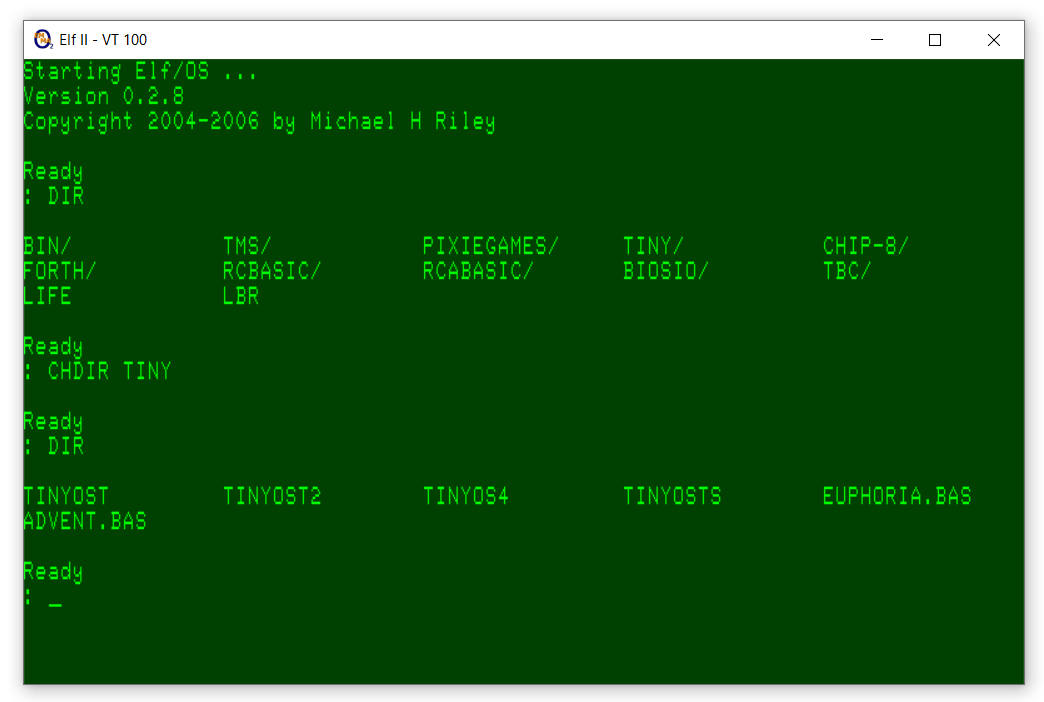
\includegraphics[width=0.95\textwidth]{./imagenes/dir_chdir.png}
  \caption{Sistema de directorios del ElfOS}
  \label{F:dir_chdir}
\end{figure}

El sistema operativo también debe incluir programas para crear y editar archivos de texto. El ElfOS posee este programa, que además brinda la posibilidad de escribir código en el lenguaje ensamblador del CDP1802, el cual puede luego ser ejecutado dentro del mismo sistema operativo, retomando su operación una vez ejecutado el código.

El sistema debe funcionar mediante el envío y recepción de caracteres (sin interfaz gráfica) mediante la comunicación con una terminal externa. Existen módulos conversores de protocolo Serial a USB que permiten realizar esta tarea.

El sistema no debe incluir conexión a internet ni ser multiusuario.

Debe contemplarse la posibilidad de que el sistema operativo a desarrollar sea de tiempo real (\textit{Real-Time Operating System RTOS}). Esto significa que debe ser capaz de aceptar y responder a eventos externos con cierto grado de fiabilidad, y en un margen de tiempo específico. Esta cualidad permite utilizar el sistema en aplicaciones industriales, donde se requiere atender a gran número de eventos externos y además controlar variables externas. La implementación de un sistema operativo de estas características permitiría utilizar la microcomputadora como un PLC.



% 9. BIBLIOGRAFÍA
\printbibliography[title={Bibliografía}]

% 8. APÉNDICES
\appendix
% si necesitamos agregar algún apéndice activamos esto
\chapter{Protocolos de Comunicación Serial}
\label{C:anexo-comunicación-serial}

\section{UART}

UART (Universal Asynchronous Receiver-Transmitter) \cite{fernandez-com-serial} es un protocolo de comunicación serial asincrónica y bidireccional full-duplex desarrollado en el año 1960 por la empresa Digital Equipment Corporation. Esta interfaz posee dos líneas de datos, RX y TX, las cuales se interconectan como lo muestra la figura~\ref{F:uart-interconexión}. UART generalmente es usada para establecer una comunicación bidireccional full-dúplex sólo entre dos dispositivos (punto a punto).

\begin{figure}[ht!]
\centering
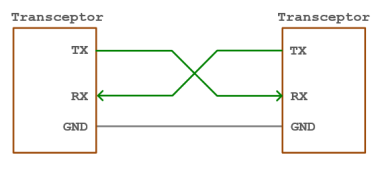
\includegraphics[width=0.55\textwidth]{./imagenes/uart-interconexión.png}
\caption{Interconexión de interfaz UART}
\label{F:uart-interconexión}
\end{figure}

La información intercambiada entre los dispositivos es mediante paquetes de datos con un formato definido como se muestra en la figura~\ref{F:uart-trama-datos}. La comunicación está sincronizada mediante los bits de START y STOP que posee el paquete, considerando que los relojes de los dispositivos transmisor y receptor operan a la misma frecuencia.

\begin{figure}[ht!]
\centering
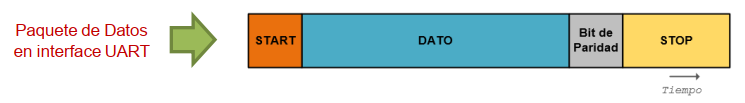
\includegraphics[width=0.9\textwidth]{./imagenes/uart-trama-datos.png}
\caption{Paquete de datos UART}
\label{F:uart-trama-datos}
\end{figure}

El paquete de datos indicado posee las siguientes configuraciones que deben efectuarse en los dispositivos que intervienen en la comunicación:

\begin{description}
   \item[Bit de START] Es el primer bit del paquete de datos y permite que el receptor reconozca el inicio de la transmisión de un paquete. Normalmente el transmisor (TX) mantiene la línea de datos en “1” cuando se encuentra en reposo. Para iniciar la transmisión pone a “0” la línea y el receptor, al detectar esto, comienza con la lectura del DATO.
   \item[DATO] Este campo del paquete puede configurarse de 5 a 9 bits. La configuración debe ser la misma para ambos dispositivos en la comunicación. Los bits son enviados uno a uno, empezando por el menos significativo y terminando con el más significativo.
   \item[Bit de Paridad] Permite al receptor verificar si los datos recibidos son correctos o no. La paridad es un sistema de comprobación de errores de bajo nivel y puede ser de paridad par o paridad impar. Debe configurarse la misma paridad en ambos dispositivos involucrados en la comunicación.
   \item[Bit de STOP] Marca el final del paquete de datos al receptor. Puede tener uno o dos bits de longitud. Debe configurarse lo mismo en ambos dispositivos. Al finalizar la transmisión, es habitual que se mantenga la línea de datos en “1” (línea en reposo).
   \item[Baud Rate (bits por segundo)]  Es un parámetro que indica la velocidad a la que se transmiten los datos y se relaciona con el reloj interno que poseen los dispositivos para la lectura/escritura de los bits que conforman el paquete de datos. Todos los dispositivos deben tener el mismo baud rate. Algunas de las velocidades estándares son 4800 bps, 9600 bps, 19200 bps, 115200 bps, etc. De estas, 9600 bps es la más utilizada.
\end{description}

\section{I\texorpdfstring{\textsuperscript{2}}{Lg}C}

I\textsuperscript{2}C (Inter-Integrated Circuit) \cite{fernandez-com-serial} es un bus de comunicación serie sincrónica bidireccional half-duplex desarrollado en el año 1982 por la empresa Philips Semiconductors. El bus I2C también es conocido con el nombre de TWI (Two Wire Interface). Este bus también posee una arquitectura Maestro-Esclavo, donde el dispositivo Maestro es el único que puede iniciar y finalizar la transmisión y también proveer la señal de reloj. En I2C los dispositivos Esclavos pueden convertirse en Maestros, pero en el bus sólo puede existir un Maestro a la vez.

El bus está compuesto de dos líneas y la conexión común de GND, como puede apreciarse en la figura~\ref{F:i2c-interconexión}. Existe una línea bidireccional para el intercambio de datos que se denomina SDA (Serial Data) y una para la señal de reloj denominada SCL (Serial Clock). Como en este bus no existen líneas de selección de esclavo, cada dispositivo Esclavo debe contar con una dirección única (código de identificación) la cual debe incluirse al dato. Esto resulta en una reducción de la velocidad de transferencia de cada byte de dato.

Las líneas SDA y SCL son del tipo drenador abierto (figura~\ref{F:i2c-entrada-y-salida}), por lo cual cada una requiere una resistencia pull-up Rp ($ \num{1.8}~\unit{\kilo\Omega} \leq Rp \leq \num{10}~\unit{\kilo\Omega} $).

\begin{figure}[ht!]
\centering
\subfloat[Interconexión de interfaz I\textsuperscript{2}C][Interconexión de interfaz I\textsuperscript{2}C]{
	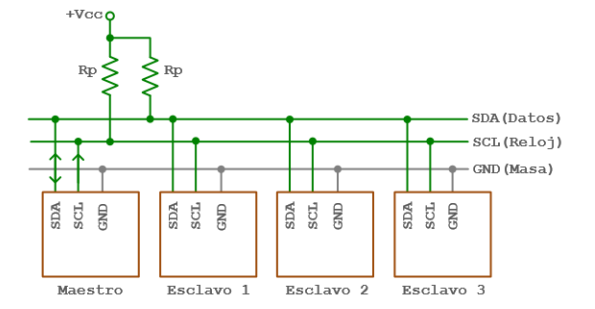
\includegraphics[width=0.65\textwidth]{./imagenes/i2c-interconexión.png}
	\label{F:i2c-interconexión}}
\\
\subfloat[Líneas SDA y SCL][Líneas SDA y SCL]{
	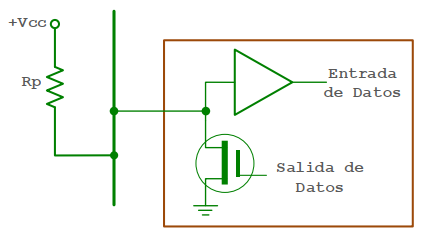
\includegraphics[width=0.43\textwidth]{./imagenes/i2c-entrada-y-salida.png}
	\label{F:i2c-entrada-y-salida}}
\caption{Interfaz I\textsuperscript{2}C}
\end{figure}

A continuación se describe un ejemplo de trama del protocolo I\textsuperscript{2}C, la cual se puede observar en la figura~\ref{F:i2c-trama-y-sec}:

\begin{itemize}
    \item El Maestro inicia la comunicación con la secuencia de inicio (START), acompañada de 7~bits que corresponden a la dirección del Esclavo con el que se desea comunicar. A esto el Maestro agrega un bit que indica si la operación será de escritura (W~=~0) o  de lectura (R~=~1). En este caso de escritura.
    \item Si el Esclavo está disponible en el bus, responde con un bit de reconocimiento (ACK) a lo anterior. Si no hay respuesta del Esclavo en cuestión, el Maestro terminará la comunicación con una secuencia de parada (STOP).
    \item Luego de que el Maestro recibe el bit de reconocimiento, el mismo envía el Dato~1 (de 8~bits) que corresponde a la dirección del registro del Esclavo donde se desea escribir. A esto el Esclavo vuelve a responder con un bit de reconocimiento (ACK). Si esto no sucede el Maestro finaliza la comunicación con una secuencia de parada (STOP).
    \item Recibido el bit de reconocimiento, el Maestro envía el Dato~2 (8~bits) que corresponde al valor que se cargará en el registro del Esclavo. Luego, este último responde con un bit de reconocimiento (ACK). Caso contrario, el Maestro finaliza la comunicación.
    \item Una vez que el Maestro ha escrito el valor correspondiente (Dato~2) en el registro deseado (Dato~1) del Esclavo, finaliza la comunicación con una secuencia de parada (STOP).
\end{itemize}

\begin{figure}[ht!]
\centering
\subfloat[Ejemplo de trama I\textsuperscript{2}C: Escritura en el registro de un Esclavo (M: Maestro; E: Esclavo)][Ejemplo de trama I\textsuperscript{2}C: Escritura en el registro de un Esclavo (M: Maestro; E: Esclavo)]{
	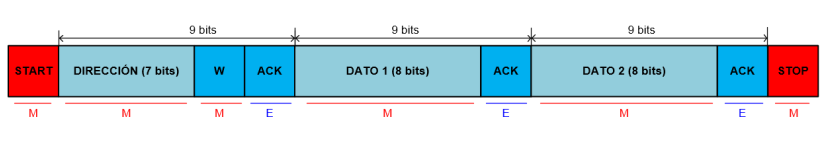
\includegraphics[width=0.98\textwidth]{./imagenes/i2c-trama.png}
	\label{F:i2c-trama}}
\\
\subfloat[Secuencia de inicio y parada I\textsuperscript{2}C][Secuencia de inicio y parada I\textsuperscript{2}C]{
	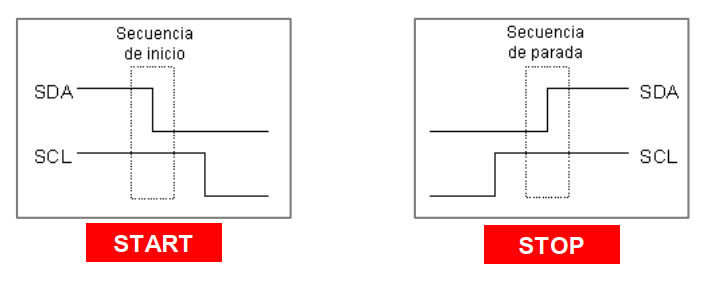
\includegraphics[width=0.7\textwidth]{./imagenes/i2c-sec-inicio-parada.png}
	\label{F:i2c-sec-inicio-parada}}
\caption{Trama y secuencia de inicio y parada I\textsuperscript{2}C}
\label{F:i2c-trama-y-sec}
\end{figure}

En la figura~\ref{F:i2c-trama-en-detalle} se encuentra ilustrada en forma más detallada la trama I\textsuperscript{2}C. A continuación se describen cada una de las subfiguras.

\paragraph{Reconocimiento de bits (figura~\ref{F:i2c-fig1}):}
El nivel lógico de la línea SDA debe ser estable cuando la línea SCL es alta. La única excepción a esta regla es la generación de secuencias de START y STOP.

\paragraph{Secuencias de START y STOP (figura~\ref{F:i2c-fig2}):}
El bus está inactivo cuando SDA~=~1 y SCL~=~1. El Maestro inicia la transmisión con una secuencia START (SDA~=$ \downarrow $  con SCL~=~1) y finaliza la misma con una secuencia de STOP (SDA~=~$ \uparrow $ con SCL~=~1). Entre una condición de START y STOP, el bus se considera ocupado y ningún otro maestro debe intentar tomar el control del bus. Si el Maestro genera una nueva secuencia de START antes de la secuencia de STOP, esto se conoce como INICIO REPETIDO (\textit{Repeated START}) y se utiliza cuando el Maestro desea iniciar una nueva transferencia sin renunciar al control del bus.

\paragraph{Paquete de Dirección (figura~\ref{F:i2c-fig3}):}
Todos los paquetes de direcciones transmitidos tienen una longitud de 9~bits y están constituidos
por:

\begin{itemize}
    \item 7~bits más significativos para la dirección del Esclavo con el cual el Maestro desea comunicarse.
    \item 1~bit para definir la operación que desea realizar el Maestro. Puede ser Lectura (R) o Escritura ($ \overline{\text{W}} $). Este bit debe ser “1” para el caso de lectura y “0” para escritura.
    \item 1~bit de reconocimiento (ACK). Este bit es generado por el Esclavo cuando reconoce la dirección enviada por el Maestro. El esclavo debe poner a “0” la línea SDA si reconoce la dirección.
\end{itemize}

\paragraph{Paquete de Datos (figura~\ref{F:i2c-fig4}):}
Todos los paquetes de datos transmitidos poseen una longitud de 9~bits y están constituidos por:

\begin{itemize}
    \item 8~bits para datos.
    \item 1~bit de reconocimiento (ACK). Este bit es generado por el receptor de los datos. El reconocimiento de la recepción se efectúa poniendo en “0” la línea SDA durante el noveno ciclo de reloj en línea SCL. Si el receptor deja la línea SDA en “1”, se señaliza un NACK. Esta señalización permite al receptor avisar que ha recibido el último byte, o por alguna razón no puede recibir más bytes.
\end{itemize}

\paragraph{Combinación de Paquetes de Dirección y Datos (figura~\ref{F:i2c-fig5}):}
 Una transmisión consiste básicamente en una secuencia de START, una dirección más bit R o W (SLA+R/W)\footnote{SLA significa dirección de esclavo (Slave Address)}, uno o más paquetes de datos y una secuencia de STOP. Pueden existir varios bytes de datos entre SLA+R/W y STOP, dependiendo del protocolo implementado por el programa del usuario.

\vspace{4cm}
~

\begin{figure}[H]
\centering
\subfloat[Reconocimiento de bits][Reconocimiento de bits]{
	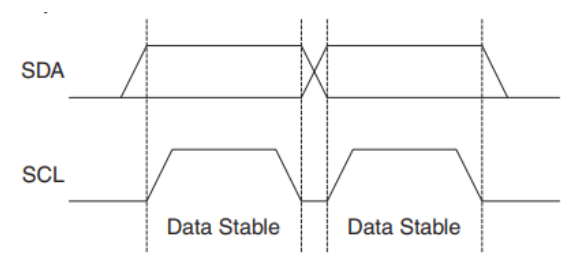
\includegraphics[width=0.41\textwidth]{./imagenes/i2c-fig1.png}
	\label{F:i2c-fig1}}
\quad
\subfloat[Secuencias de START y STOP][Secuencias de START y STOP]{
	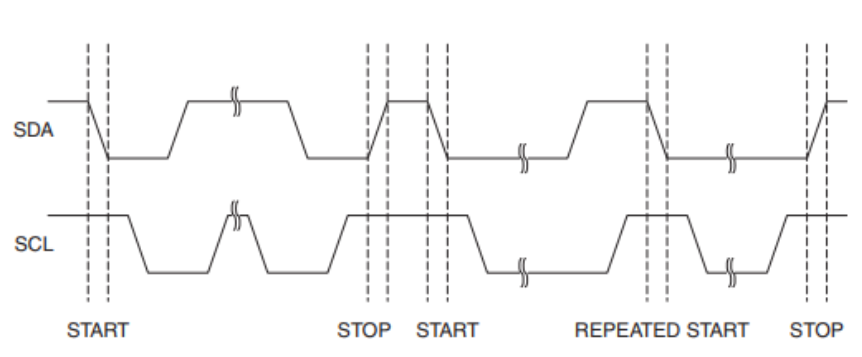
\includegraphics[width=0.53\textwidth]{./imagenes/i2c-fig2.png}
	\label{F:i2c-fig2}}
\\
\subfloat[Paquete de Dirección][Paquete de Dirección]{
	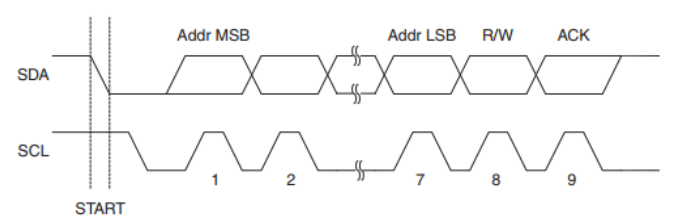
\includegraphics[width=0.62\textwidth]{./imagenes/i2c-fig3.png}
	\label{F:i2c-fig3}}
	\\
\subfloat[Paquete de Datos][Paquete de Datos]{
	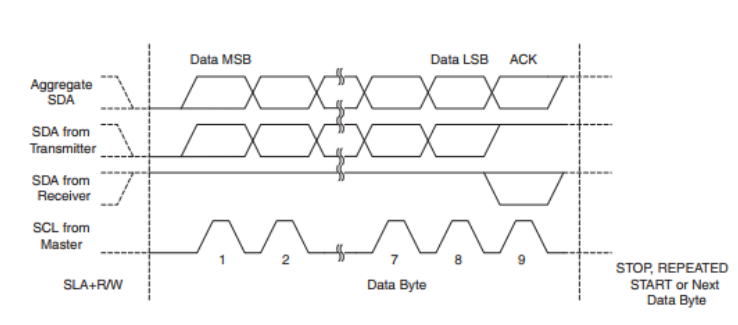
\includegraphics[width=0.75\textwidth]{./imagenes/i2c-fig4.png}
	\label{F:i2c-fig4}}
	\\
\subfloat[Combinación de Paquetes de Dirección y Datos][Combinación de Paquetes de Dirección y Datos]{
	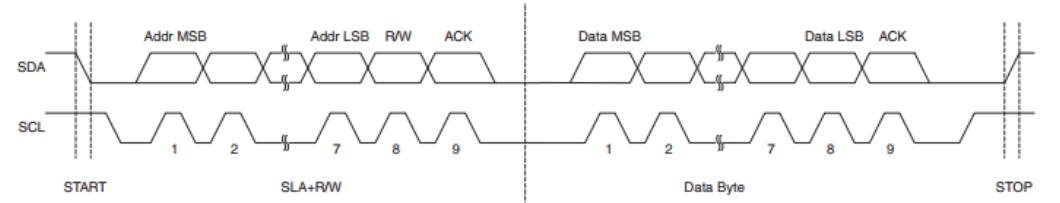
\includegraphics[width=0.95\textwidth]{./imagenes/i2c-fig5.png}
	\label{F:i2c-fig5}}
\caption{Trama I\textsuperscript{2}C en detalle}
\label{F:i2c-trama-en-detalle}
\end{figure}

\section{SPI}

SPI (Serial Peripheral Interface) \cite{fernandez-com-serial} es un bus de comunicación serie sincrónica bidireccional full-duplex desarrollado en el año 1980 por la empresa Motorola. En el bus SPI hay un dispositivo Maestro y uno o más Esclavos. El Maestro es el único encargado de iniciar y finalizar la comunicación en cualquiera de las direcciones y también genera la señal de reloj de sincronización. Este bus se encuentra compuesto por las siguientes cuatro líneas más la línea común de GND:
\clearpage
\begin{description}
   \item[MOSI (Master Out Slave In):] Esta línea lleva los datos desde el Maestro a los Esclavos.
   \item[MISO (Master In Slave Out):] Lleva los datos desde los Esclavos al Maestro.
   \item[CLK (Clock):] Esta línea lleva los pulsos de reloj desde el Maestro a los Esclavos.
   \item[$ \overline{\text{SS}} $ (Slave Select):] Es la línea mediante la cual el Maestro selecciona al Esclavo con el cual quiere comunicarse. Si hay varios esclavos, pueden existir varias líneas de selección de esclavos.
\end{description}

\begin{figure}[ht!]
\centering
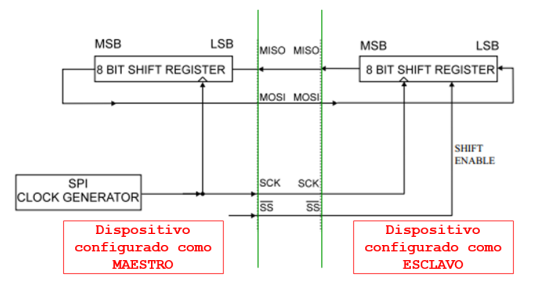
\includegraphics[width=0.8\textwidth]{./imagenes/spi-interconexión.png}
\caption{Interconexión interfaz SPI}
\label{F:spi-interconexión}
\end{figure}


\paragraph{Operación:}
El sistema de comunicación SPI de la figura~\ref{F:spi-interconexión} posee dos registros de desplazamiento (de 8 bits c/u) y un generador de reloj maestro. El maestro SPI inicia el ciclo de comunicación cuando pone en bajo el pin $ \overline{\text{SS}} $. El maestro y el esclavo preparan los datos para ser enviados en sus respectivos registros de desplazamiento, y el maestro genera los pulsos de reloj requeridos en la línea CLK para intercambiar los datos. Estos últimos van de Maestro a Esclavo a través de la línea MOSI y de Esclavo a Maestro a través de MISO. Después de cada paquete de datos (8 bits), el maestro sincronizará al esclavo poniendo en alto la línea de selección $ \overline{\text{SS}} $.
\chapter{Formato Intel (Archivo .hex)}
\label{C:anexo_formato_intel}

El formato de archivo de objeto hexadecimal de Intel, el formato hexadecimal de Intel o Intellec Hex es un formato de archivo que transmite información binaria en forma de texto ASCII \cite{dot-hex-file}. Se usa comúnmente para programar microcontroladores, EPROM y otros tipos de dispositivos lógicos programables y emuladores de hardware. En una aplicación típica, un compilador o ensamblador convierte el código fuente de un programa (como en lenguaje C o ensamblador) en código de máquina y lo envía a un archivo \texttt{.hex}. Algunos también lo usan como un formato contenedor que contiene paquetes de datos de transmisión. Las extensiones de archivo comunes utilizadas para los archivos resultantes son \texttt{.hex} o \texttt{.H86}. Luego, un programador lee el archivo \texttt{.hex} para escribir el código máquina en una memoria o se transfiere al sistema de destino para su carga y ejecución.

\begin{figure}[ht!]
\centering
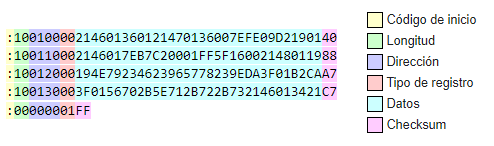
\includegraphics[width=0.7\textwidth]{./imagenes/hex-ejemplo.png}
\caption{ejemplo de archivo \texttt{.hex}}
\label{F:hex-ejemplo}
\end{figure}

\begin{description}
   \item[Código de inicio] El código de inicio utilizado es dos puntos ":"
   \item[Longitud del registro] Dos dígitos hexadecimales con la cantidad de bytes del campo de datos.
   \item[Dirección] Cuatro dígitos hexadecimales, con la dirección de inicio de los datos.
   \item[Tipo de registro] Dos dígitos hexadecimales, de 00 a 05, definen el tipo del campo de datos.
   \item[Datos] Duplas de dígitos hexadecimales que contienen los datos
   \item[Checksum] Dos dígitos hexadecimales con el complemento a dos de la suma de todos los campos anteriores, salvo el ":"
\end{description}

Hay seis tipos de registros, los mismos se describen a continuación:

\begin{description}
    \item[00] \underline{Datos}: La \textit{Longitud de registro} especifica el número de bytes de datos en el registro. El ejemplo tiene \colorbox{YellowGreen}{0B} (once) bytes de datos. La dirección inicial de 16 bits para los datos (en el ejemplo, en direcciones que comienzan en \colorbox{Periwinkle}{0010}) y los datos (\colorbox{SkyBlue}{61}, \colorbox{SkyBlue}{64}, \colorbox{SkyBlue}{64}, \colorbox{SkyBlue}{72}, \colorbox{SkyBlue}{65}, \colorbox{SkyBlue}{73}, \colorbox{SkyBlue}{73}, \colorbox{SkyBlue}{20}, \colorbox{SkyBlue}{67}, \colorbox{SkyBlue}{61}, \colorbox{SkyBlue}{70}).
    
    \underline{Ejemplo:} \colorbox{GreenYellow}{:}\colorbox{LimeGreen}{0B}\colorbox{Periwinkle}{0010}\colorbox{Peach}{00}\colorbox{SkyBlue}{6164647265737320676170}\colorbox{Lavender}{A7}
    
    \item[01] \underline{Fin de archivo}: Debe ocurrir exactamente una vez por archivo en el último registro del archivo. La Longitud siempre es \colorbox{YellowGreen}{00}, el campo de dirección suele ser \colorbox{Periwinkle}{0000} y se omite el campo de datos.
    
    \underline{Ejemplo:} \colorbox{GreenYellow}{:}\colorbox{LimeGreen}{00}\colorbox{Periwinkle}{0000}\colorbox{Peach}{01}\colorbox{Lavender}{FF}
    
    \item[02] \underline{Dirección Extendida de Segmento}: El Tipo de Registro siempre es \colorbox{Peach}{02}, el campo de dirección (normalmente \colorbox{Periwinkle}{0000}) se ignora y el campo de datos contiene una dirección base de segmento de 16~bits. Esto se multiplica por 16 y se suma a cada dirección de registro de datos subsiguiente para formar la dirección inicial de los datos. Esto permite direccionar hasta un mebibyte (1048576~bytes) de espacio de direcciones.

    \underline{Ejemplo:} \colorbox{GreenYellow}{:}\colorbox{LimeGreen}{02}\colorbox{Periwinkle}{0000}\colorbox{Peach}{02}\colorbox{SkyBlue}{1200}\colorbox{Lavender}{EA}
    
    \item[03] \underline{Dirección de Comienzo de Segmento}: Para procesadores 80x86, especifica la dirección de ejecución inicial. El Tipo de Registro siempre es \colorbox{Peach}{04}, el campo de dirección es \colorbox{Periwinkle}{0000} y los dos primeros bytes de datos son el valor CS, los dos últimos son el valor IP.
    
    
    \underline{Ejemplo:} \colorbox{GreenYellow}{:}\colorbox{LimeGreen}{04}\colorbox{Periwinkle}{0000}\colorbox{Peach}{03}\colorbox{SkyBlue}{00003800}\colorbox{Lavender}{C1}
    
    \item[04] \underline{Dirección Lineal Extendida}: Permite direccionamiento de 32~bits (hasta 4~GiB). La Longitud de bytes siempre es \colorbox{LimeGreen}{02} y el campo de dirección se ignora (normalmente \colorbox{Periwinkle}{0000}). Los dos bytes de datos especifican los 16 bits superiores de la dirección absoluta de 32~bits para todos los registros de tipo \colorbox{Peach}{00} posteriores; estos bits de dirección superiores se aplican hasta el siguiente registro \colorbox{Peach}{04}. La dirección absoluta para un registro de tipo \colorbox{Peach}{00} se forma combinando los 16~bits de dirección superiores del registro \colorbox{Peach}{04} más reciente con los 16~bits de dirección inferiores del registro \colorbox{Peach}{00}. Si un registro de tipo \colorbox{Peach}{00} no está precedido por ningún registro de tipo \colorbox{Peach}{04}, sus 16~bits de dirección superiores se establecen de forma predeterminada en \colorbox{Periwinkle}{0000}.
    
    \underline{Ejemplo:} \colorbox{GreenYellow}{:}\colorbox{LimeGreen}{02}\colorbox{Periwinkle}{0000}\colorbox{Peach}{04}\colorbox{SkyBlue}{FFFF}\colorbox{Lavender}{FC}
    
    \item[05] \underline{Comienzo de Dirección Lineal}: La Longitud de bytes siempre es \colorbox{LimeGreen}{04}, el campo de dirección es \colorbox{Periwinkle}{0000}. Los cuatro bytes de datos representan un valor de dirección de 32~bits. En el caso de las CPU que lo soportan, esta dirección de 32~bits es la dirección de ejecución inicial).
    
    \underline{Ejemplo:} \colorbox{GreenYellow}{:}\colorbox{LimeGreen}{04}\colorbox{Periwinkle}{0000}\colorbox{Peach}{05}\colorbox{SkyBlue}{000000CD}\colorbox{Lavender}{2A}
    
\end{description}
\chapter{Programas escritos para el sistema mínimo}
\label{C:anexo-programas-sistema-mínimo}

En este anexo se encuentra el código fuente de los programas escritos para el sistema mínimo.

\section{Programa 1: Parpadeo LED Q}
\label{C:anexo-prog-1}

\clearpage

\footnotesize
\lstinputlisting[language=CDP1802, caption=Programa 1]{codigo/1_qblink_test.asm}
\clearpage

\section{Programa 2: LED Q se enciende al presionar pulsador}
\label{C:anexo-prog-2}

\lstinputlisting[language=CDP1802, caption=Programa 2]{codigo/2_qInPutTurnOn.asm}
\clearpage

\section{Programa 3: LED Q parpadea al presionar pulsador}
\label{C:anexo-prog-3}

\lstinputlisting[language=CDP1802, caption=Programa 3]{codigo/3_qblinkIfPressed.asm}
\clearpage

\section{Programa 4: Transmisión serial de caracteres}
\label{C:anexo-prog-4}

\lstinputlisting[language=CDP1802, caption=Programa 4]{codigo/send_characters.asm}
\normalsize
\chapter{Esquemas circuitales y circuitos impresos}

En este apéndice se incluyen los esquemáticos presentados dentro del cuerpo del informe, pero en el tamaño de hoja original.


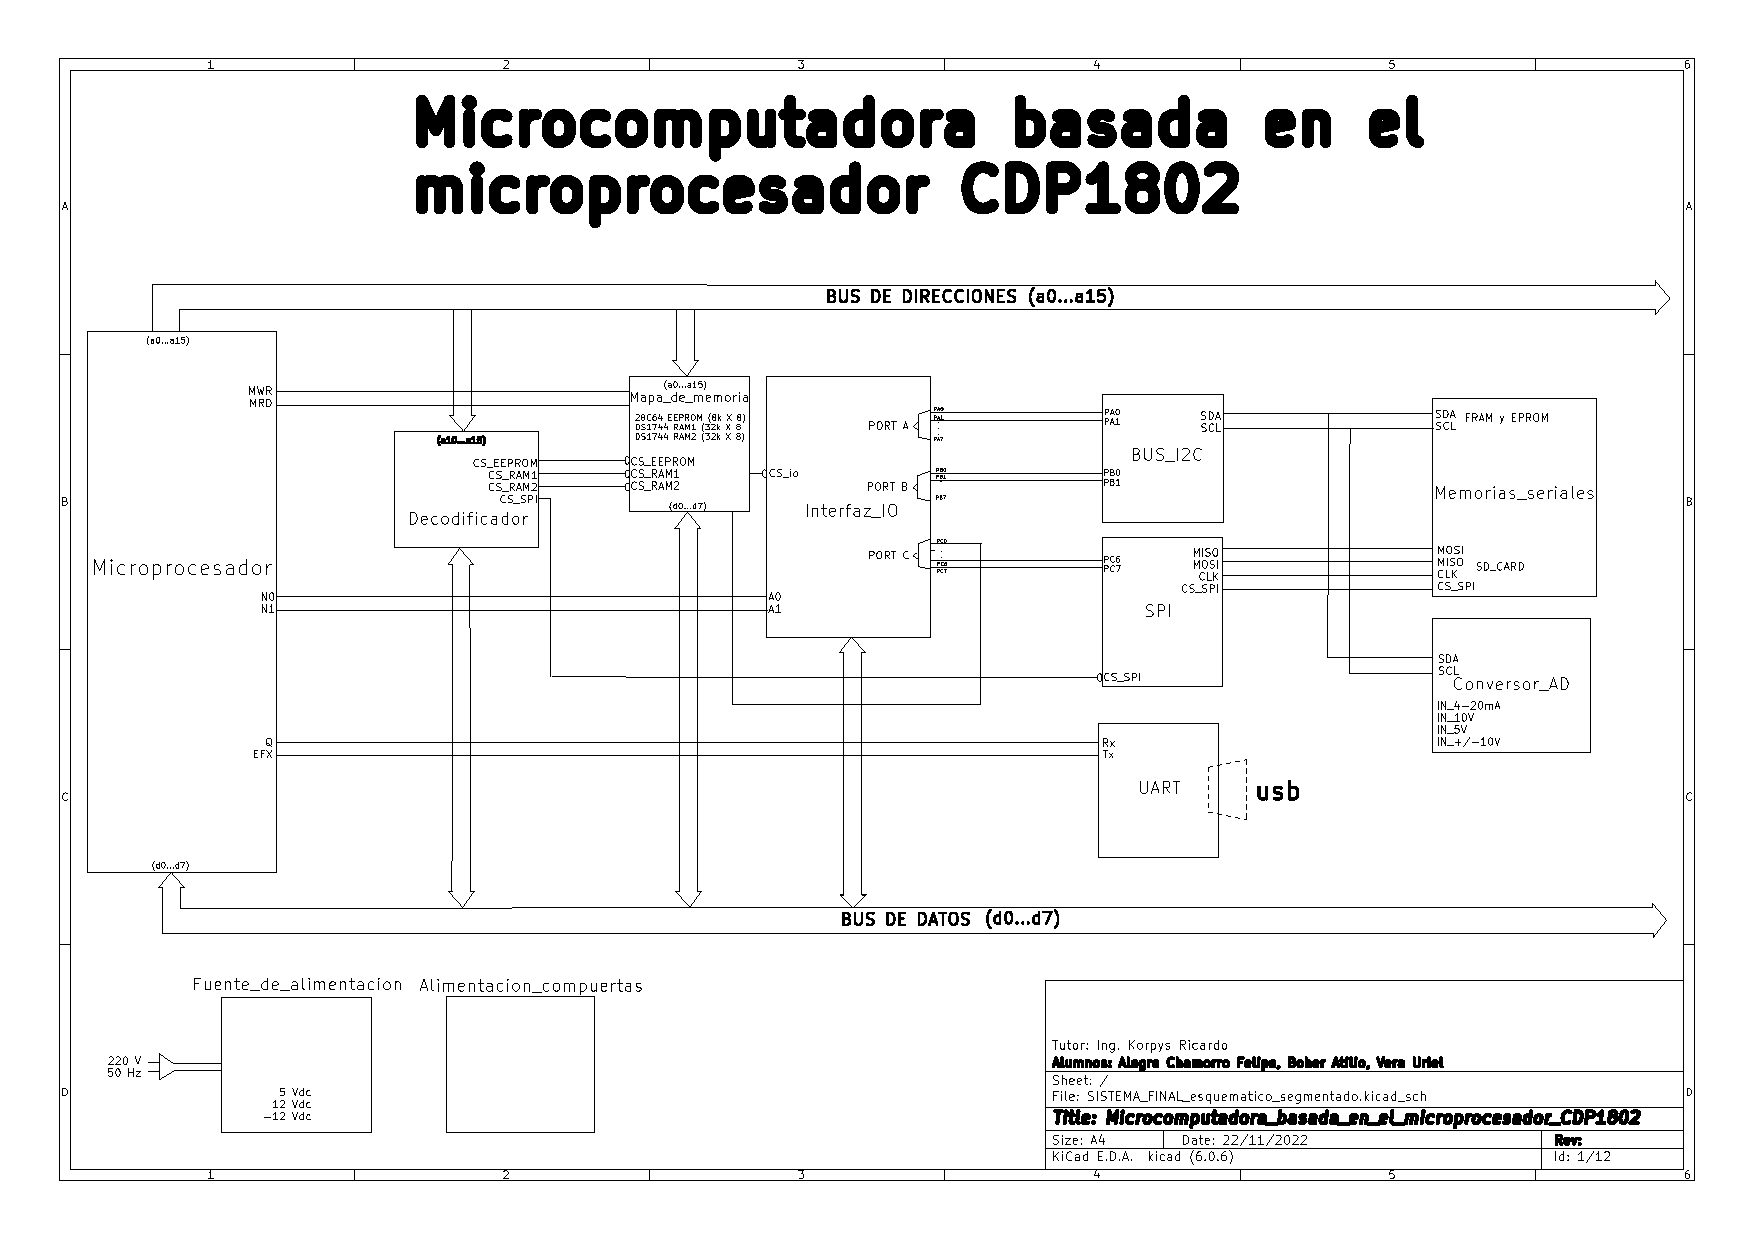
\includepdf[fitpaper, angle=90]{./imagenes/EsquematicosSF/Esquematico (1).pdf}
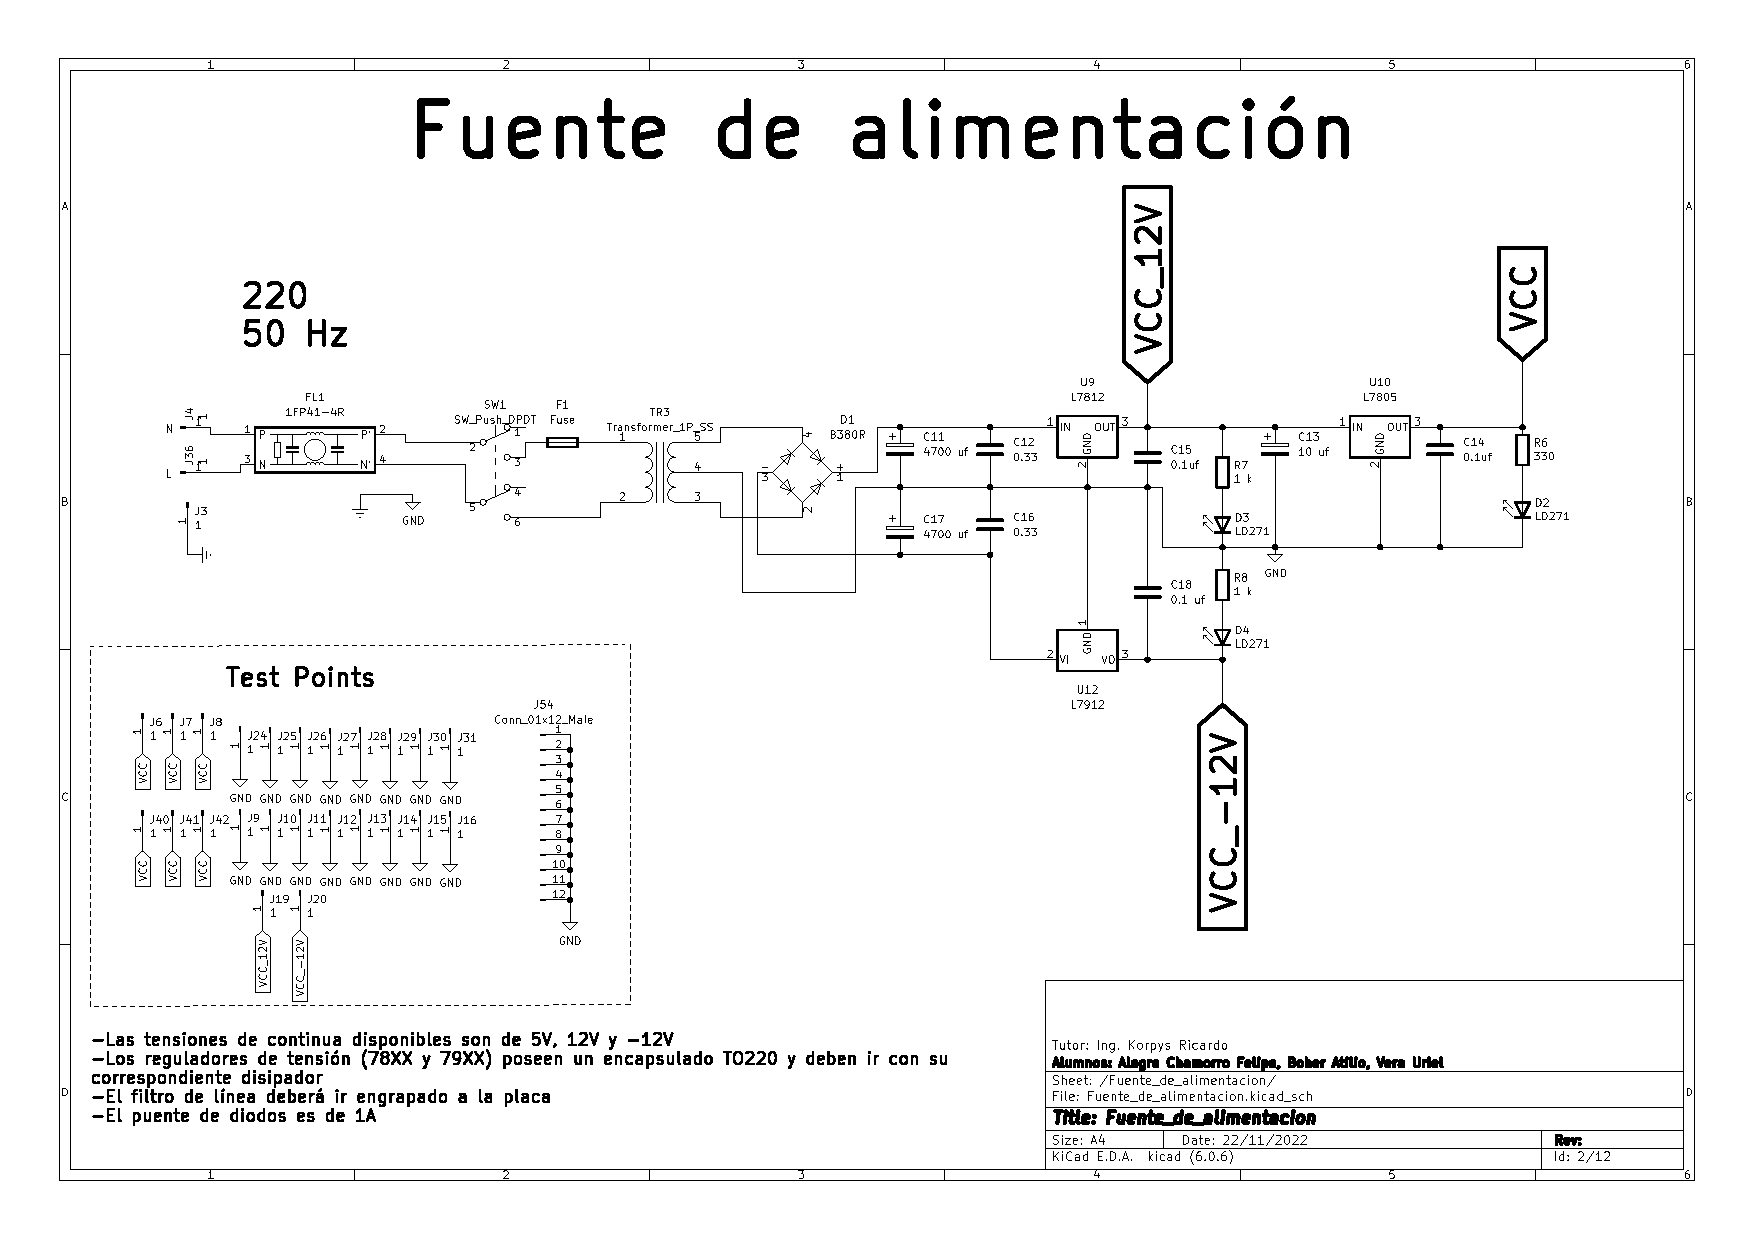
\includepdf[fitpaper, angle=90]{./imagenes/EsquematicosSF/Esquematico (2).pdf}
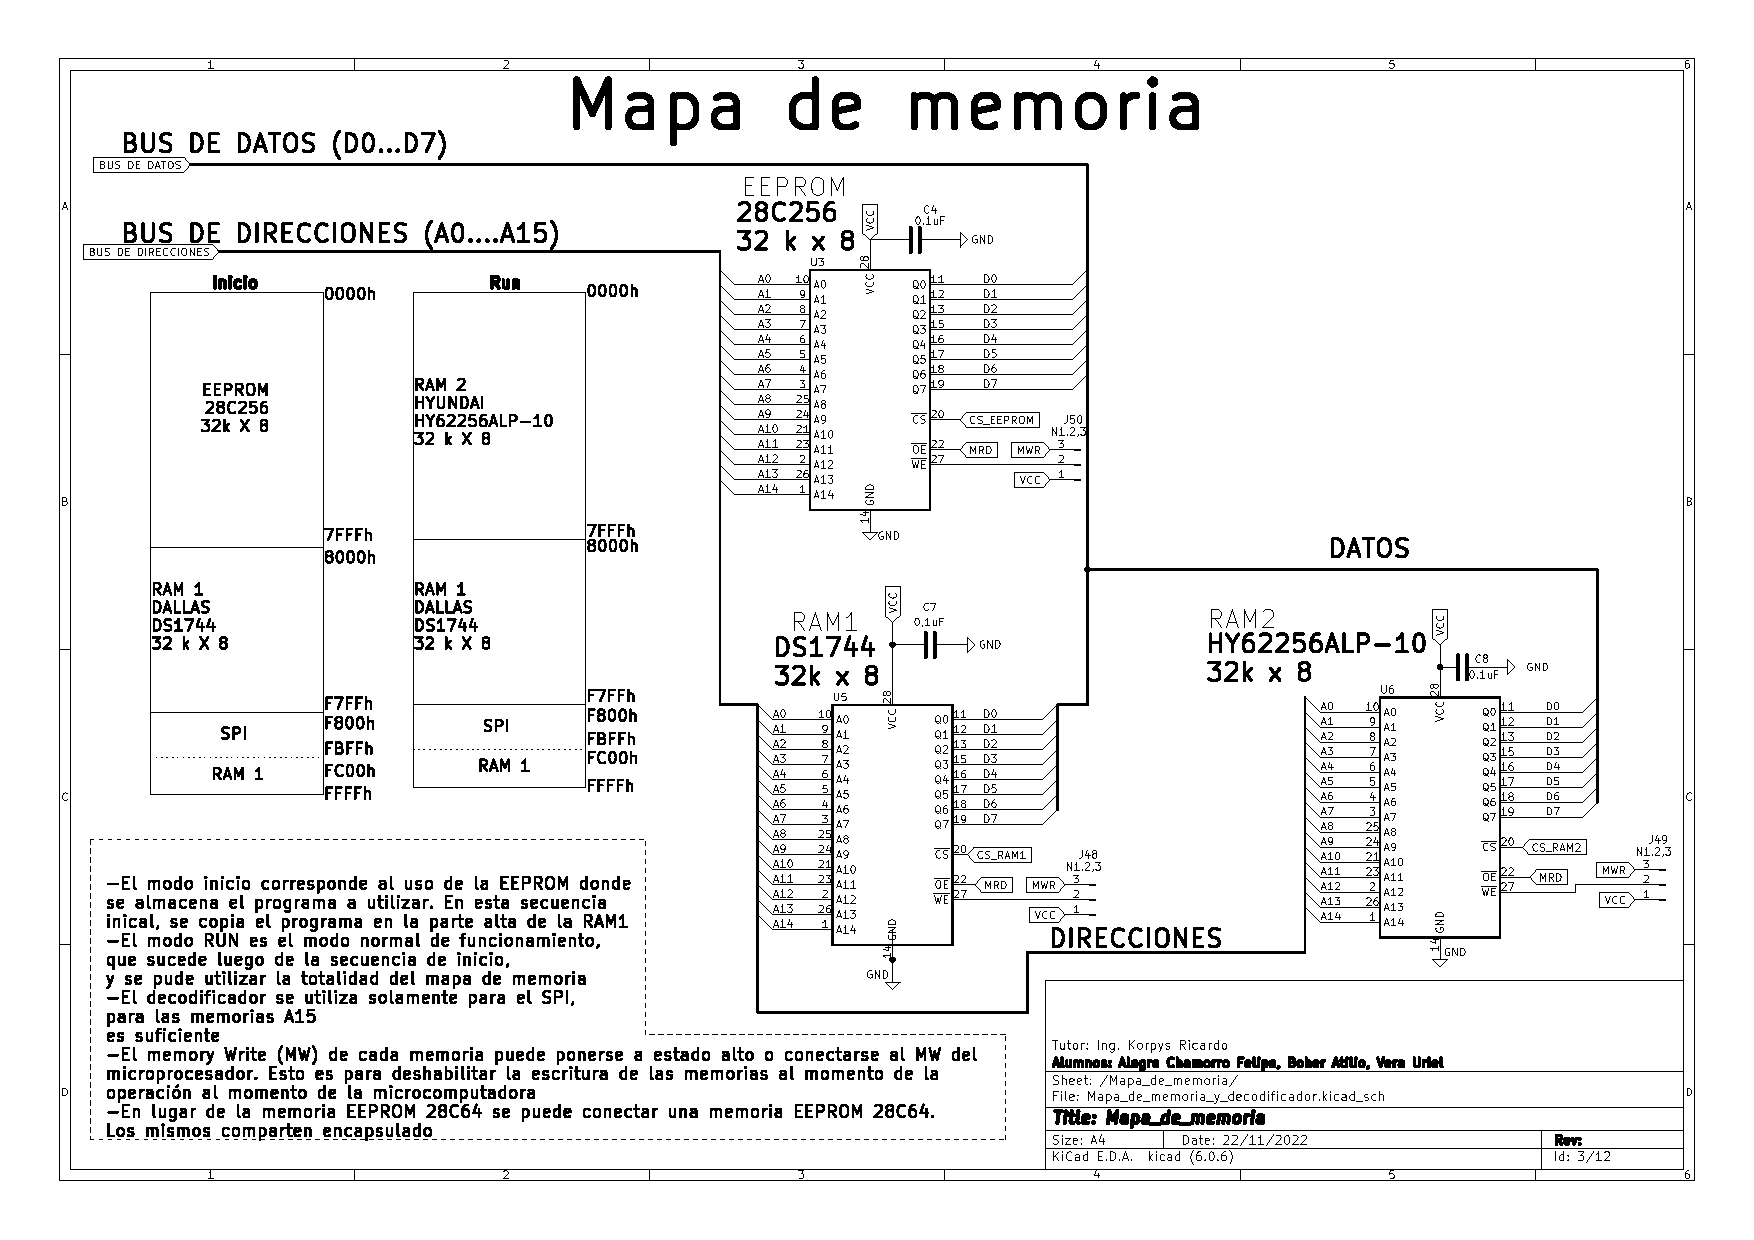
\includepdf[fitpaper, angle=90]{./imagenes/EsquematicosSF/Esquematico (3).pdf}
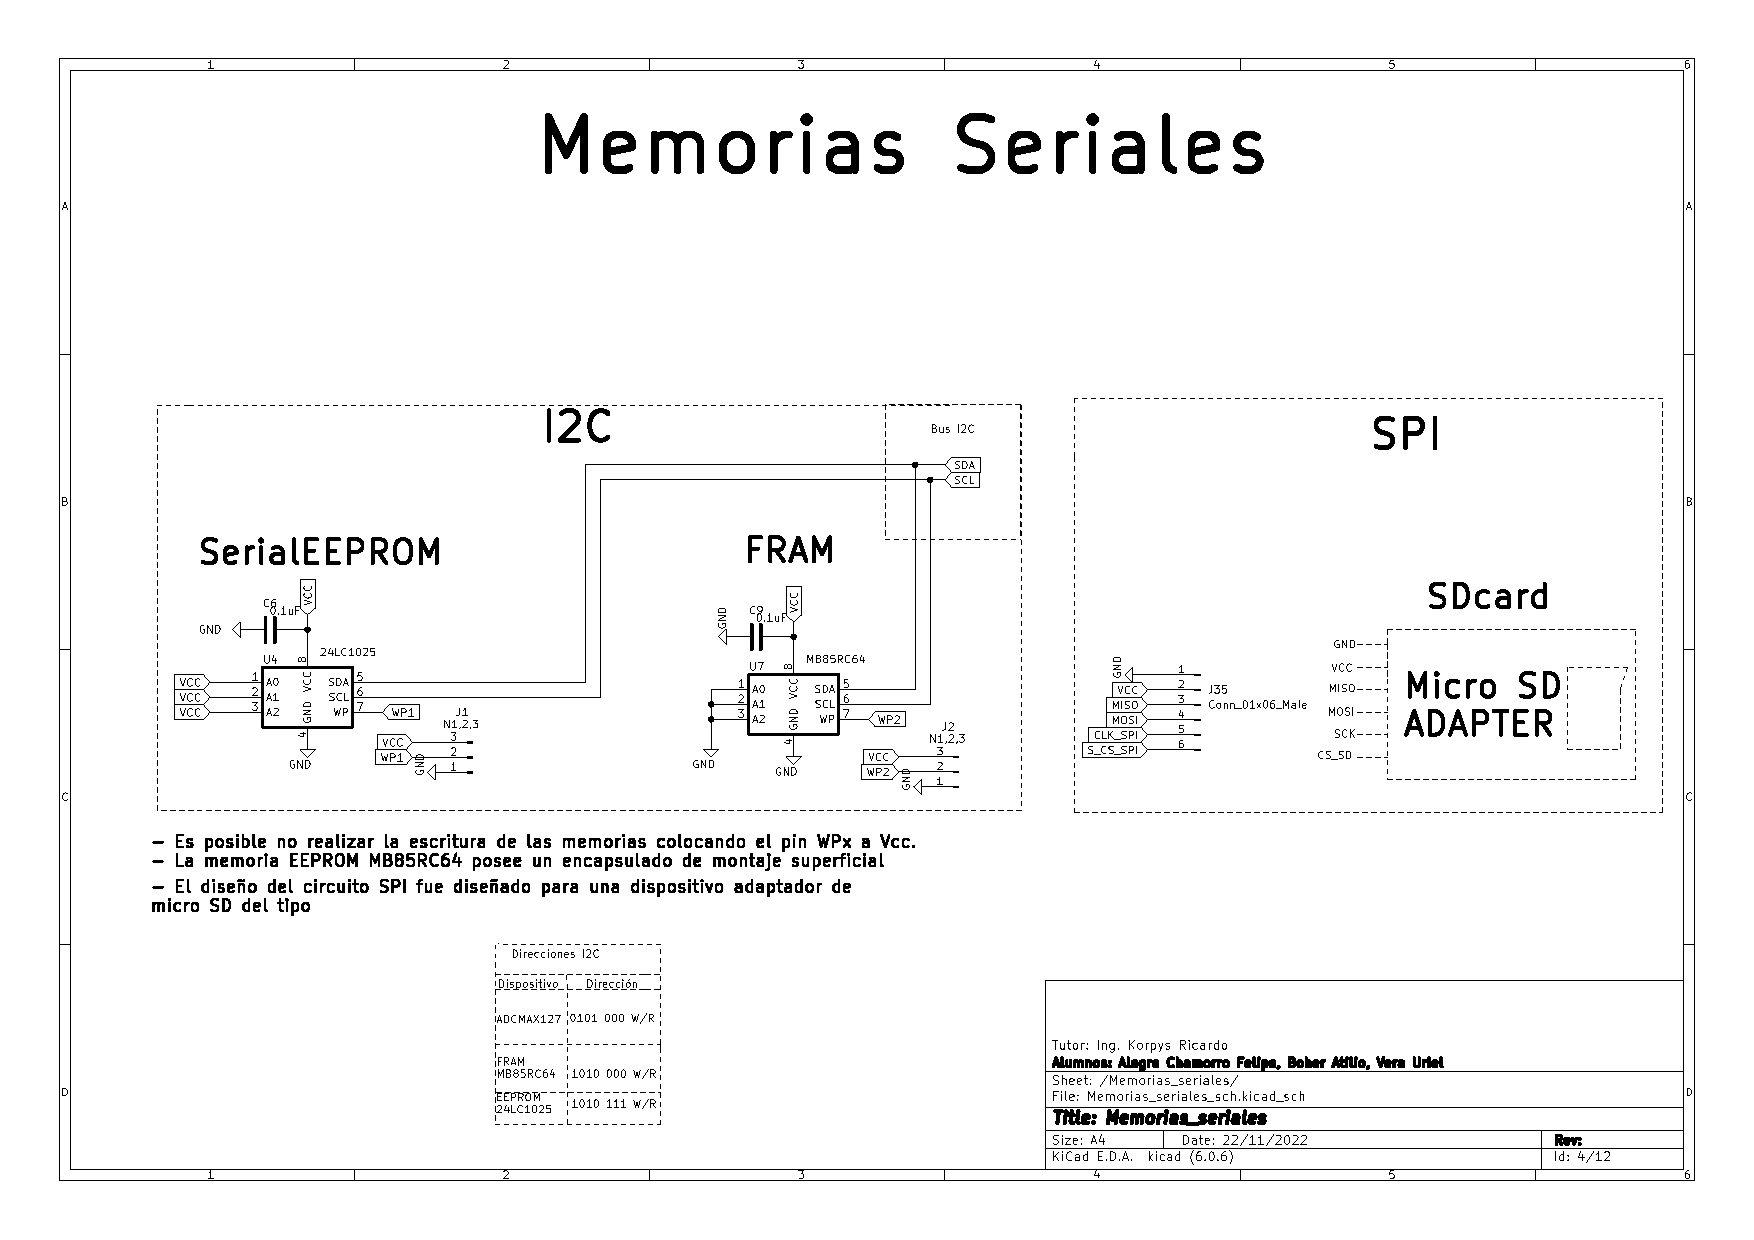
\includepdf[fitpaper, angle=90]{./imagenes/EsquematicosSF/Esquematico (4).pdf}
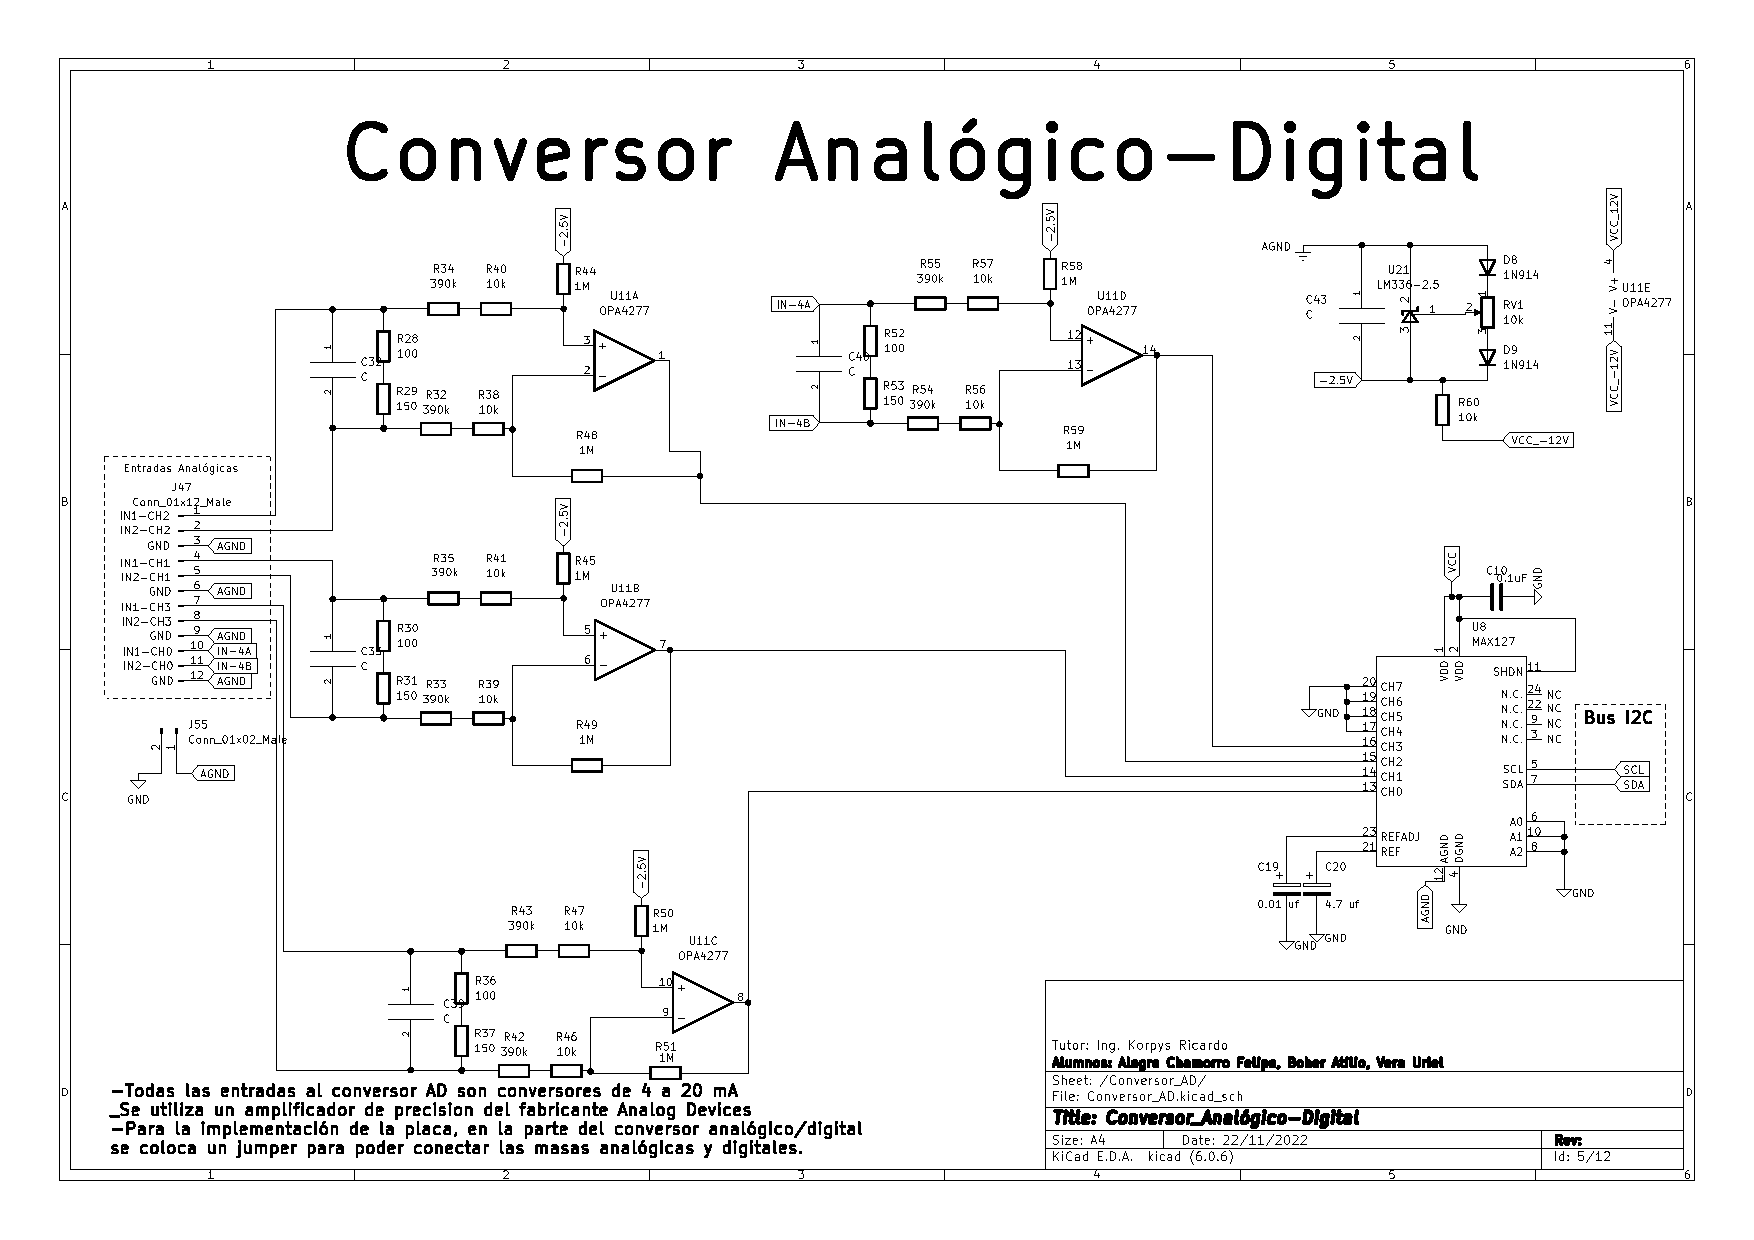
\includepdf[fitpaper, angle=90]{./imagenes/EsquematicosSF/Esquematico (5).pdf}
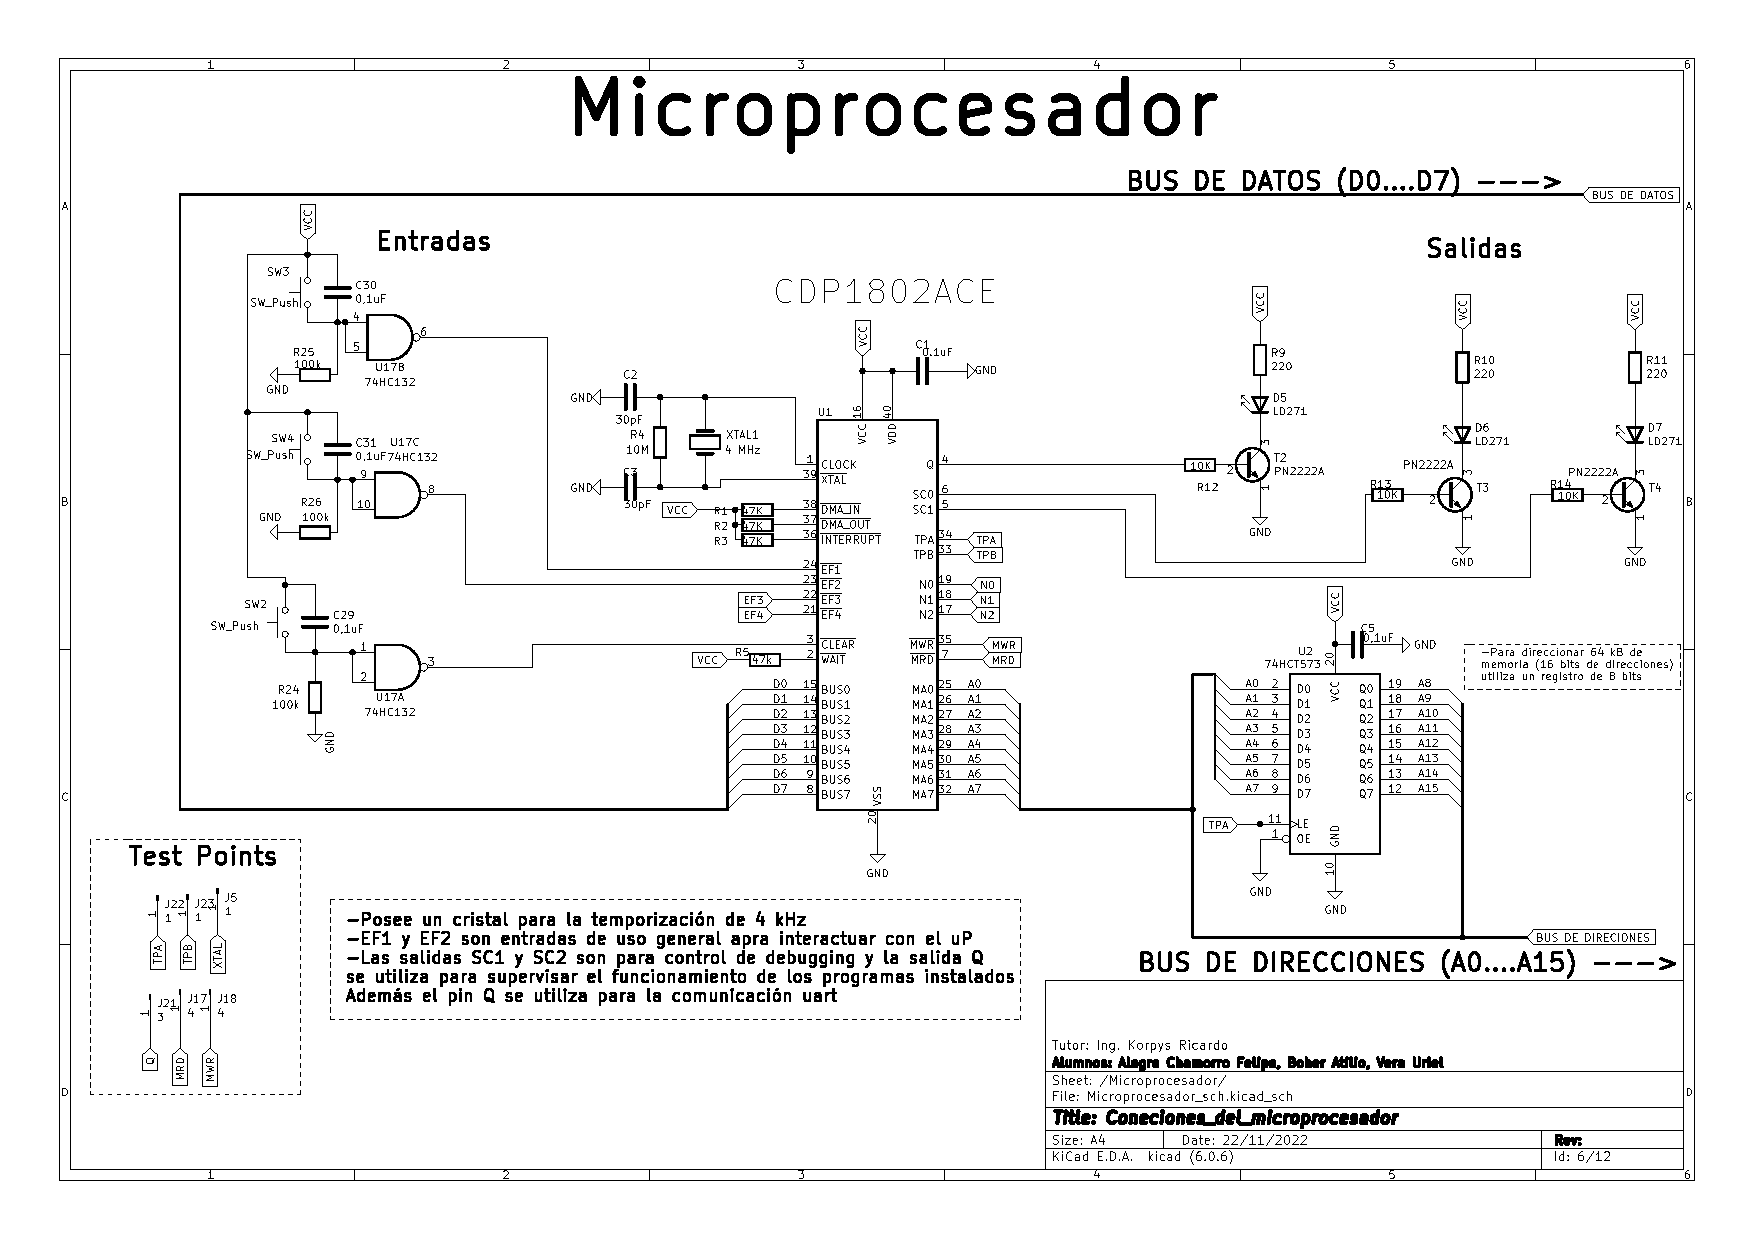
\includepdf[fitpaper, angle=90]{./imagenes/EsquematicosSF/Esquematico (6).pdf}
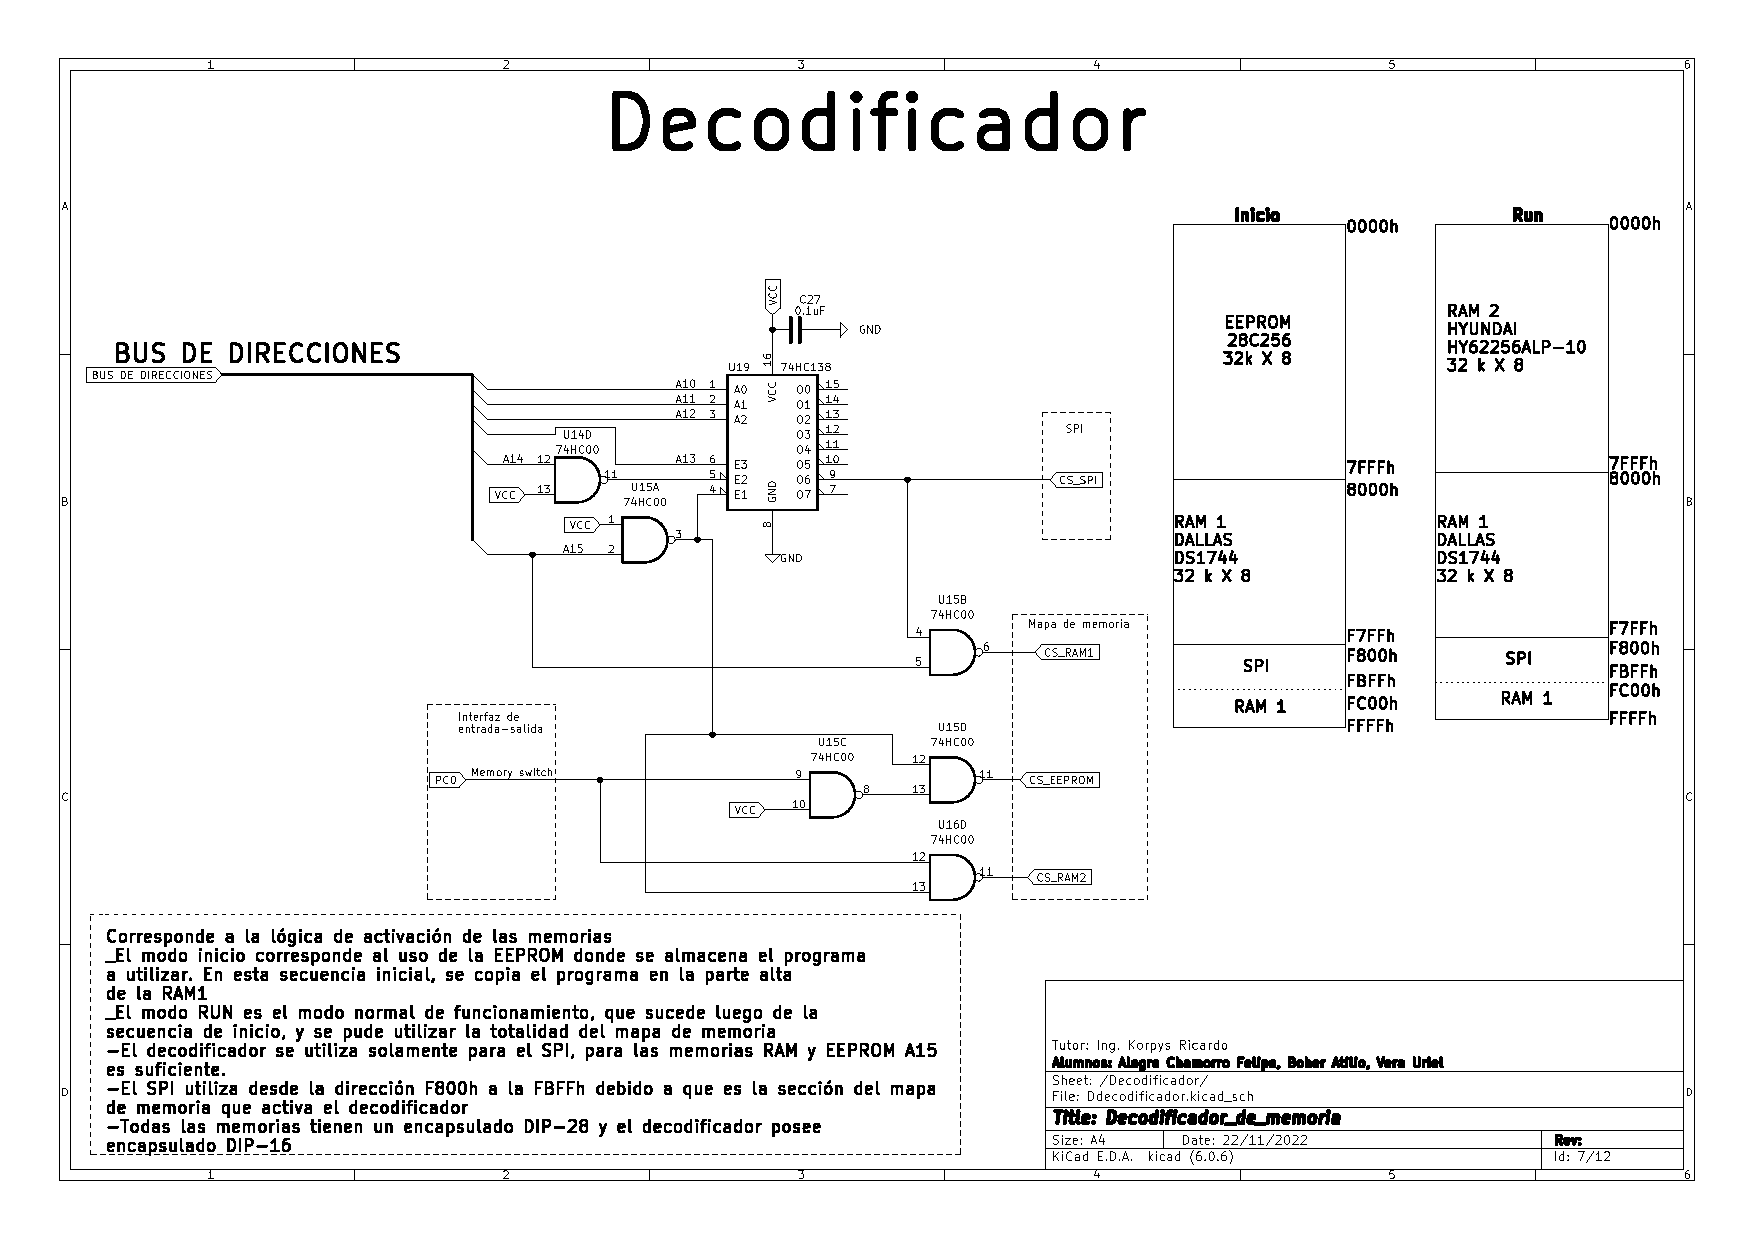
\includepdf[fitpaper, angle=90]{./imagenes/EsquematicosSF/Esquematico (7).pdf}
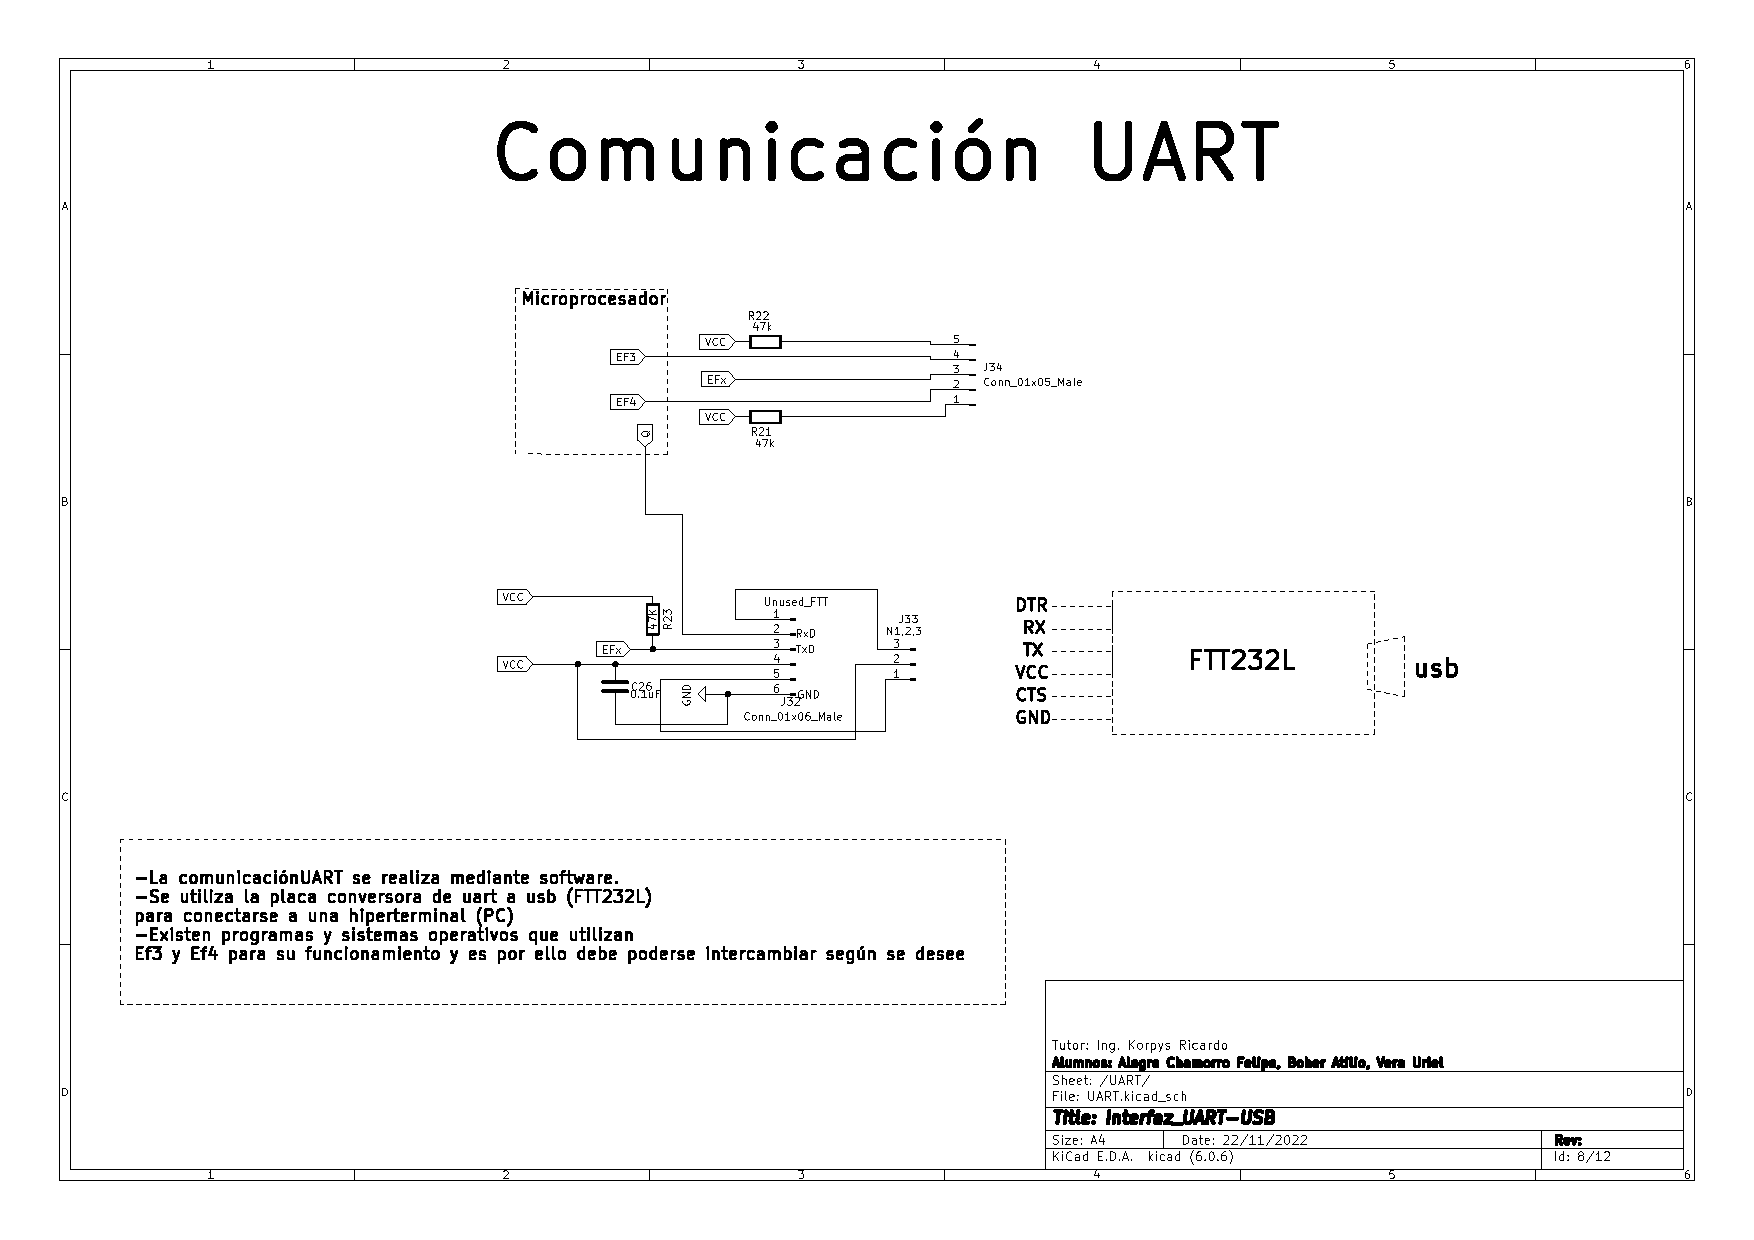
\includepdf[fitpaper, angle=90]{./imagenes/EsquematicosSF/Esquematico (8).pdf}
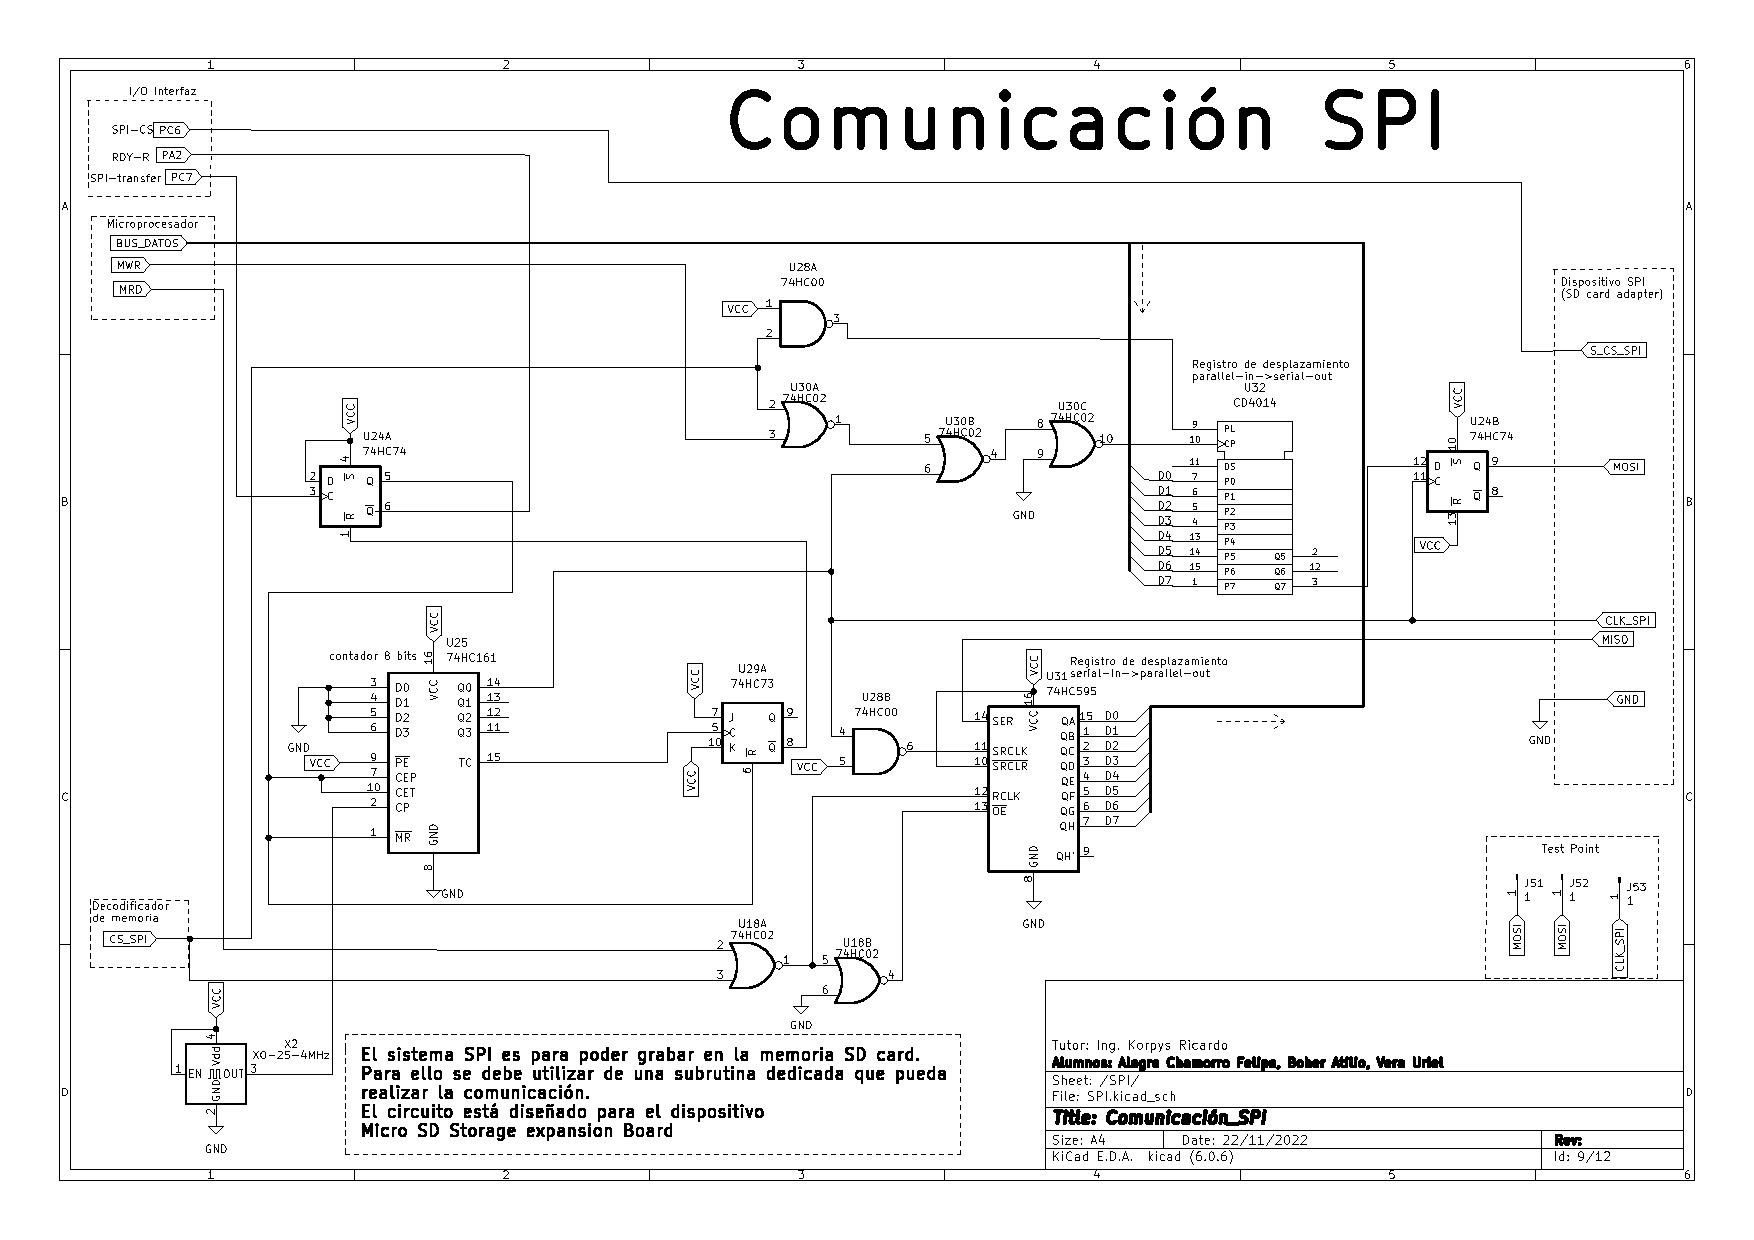
\includepdf[fitpaper, angle=90]{./imagenes/EsquematicosSF/Esquematico (9).pdf}
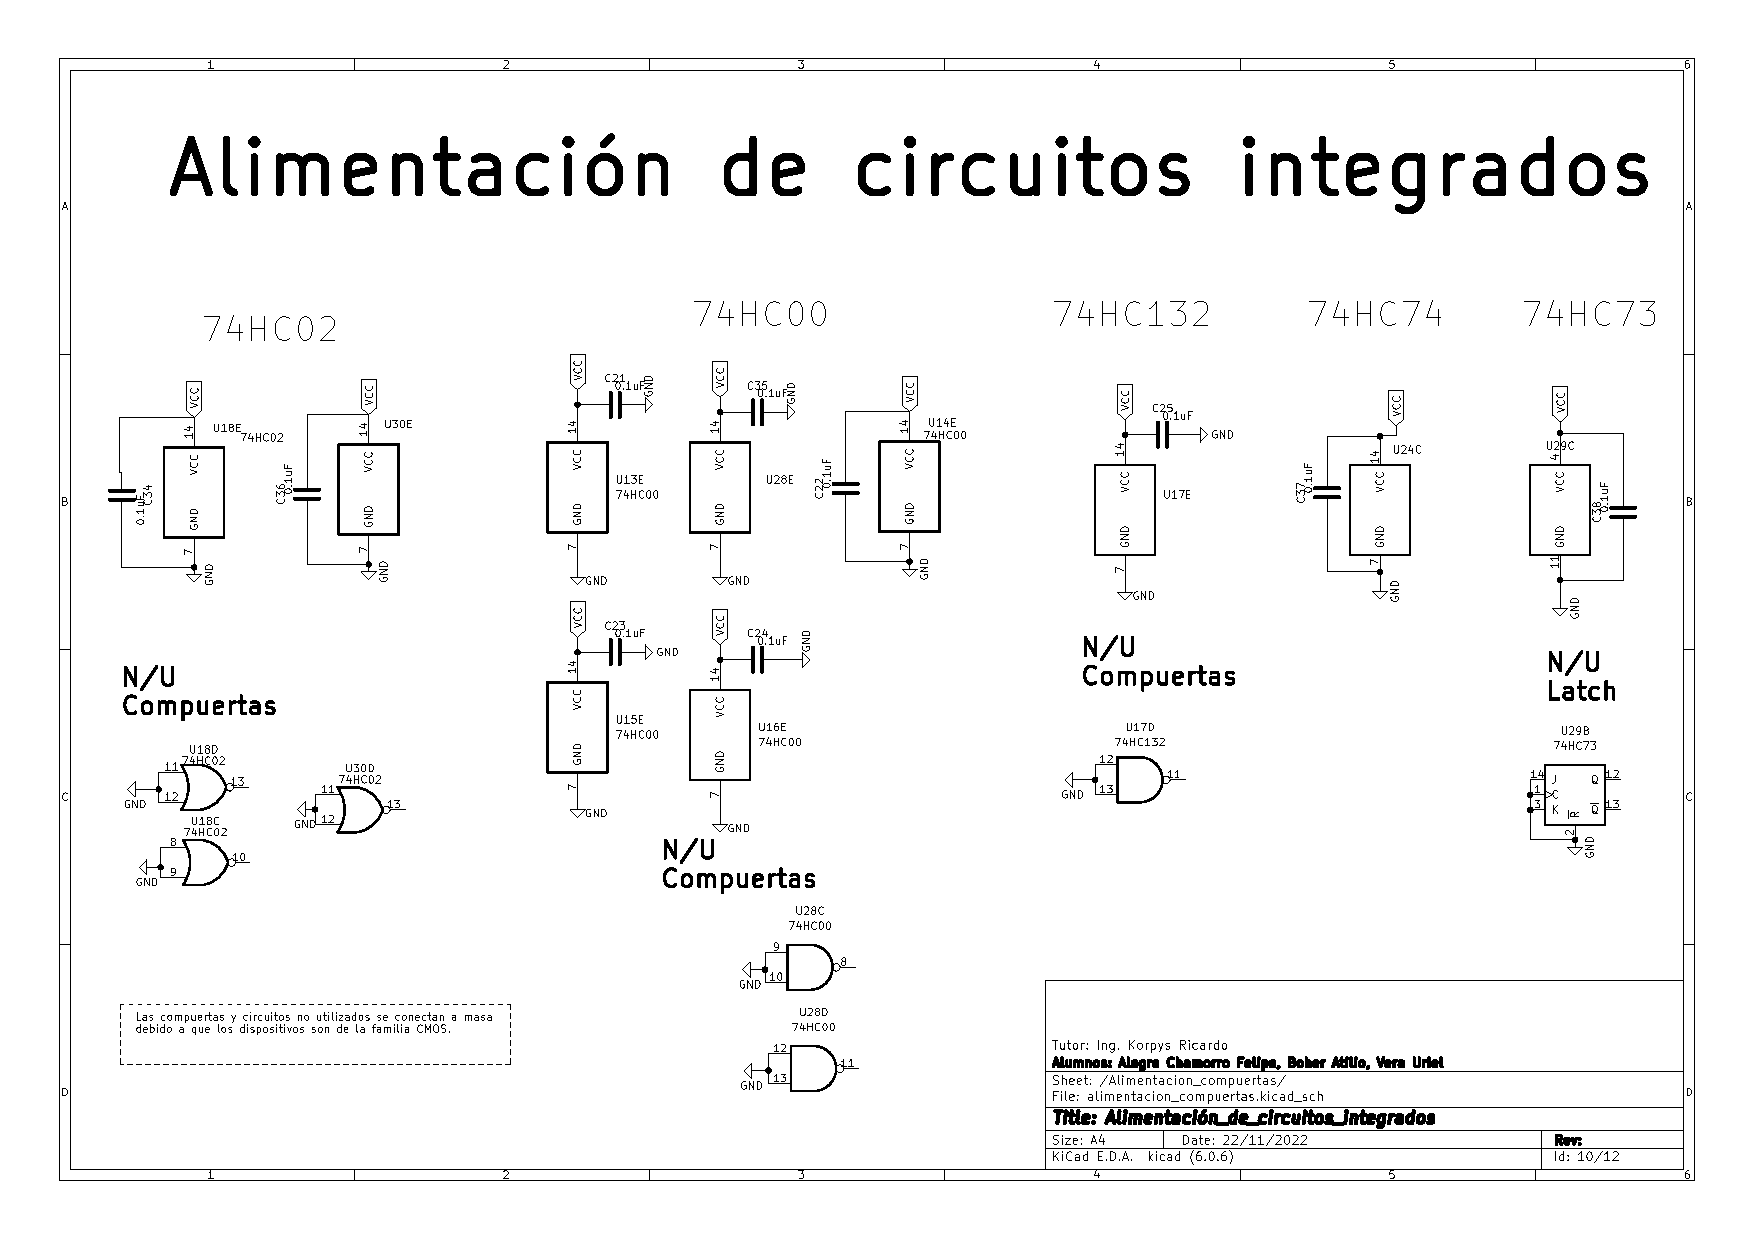
\includepdf[fitpaper, angle=90]{./imagenes/EsquematicosSF/Esquematico (10).pdf}
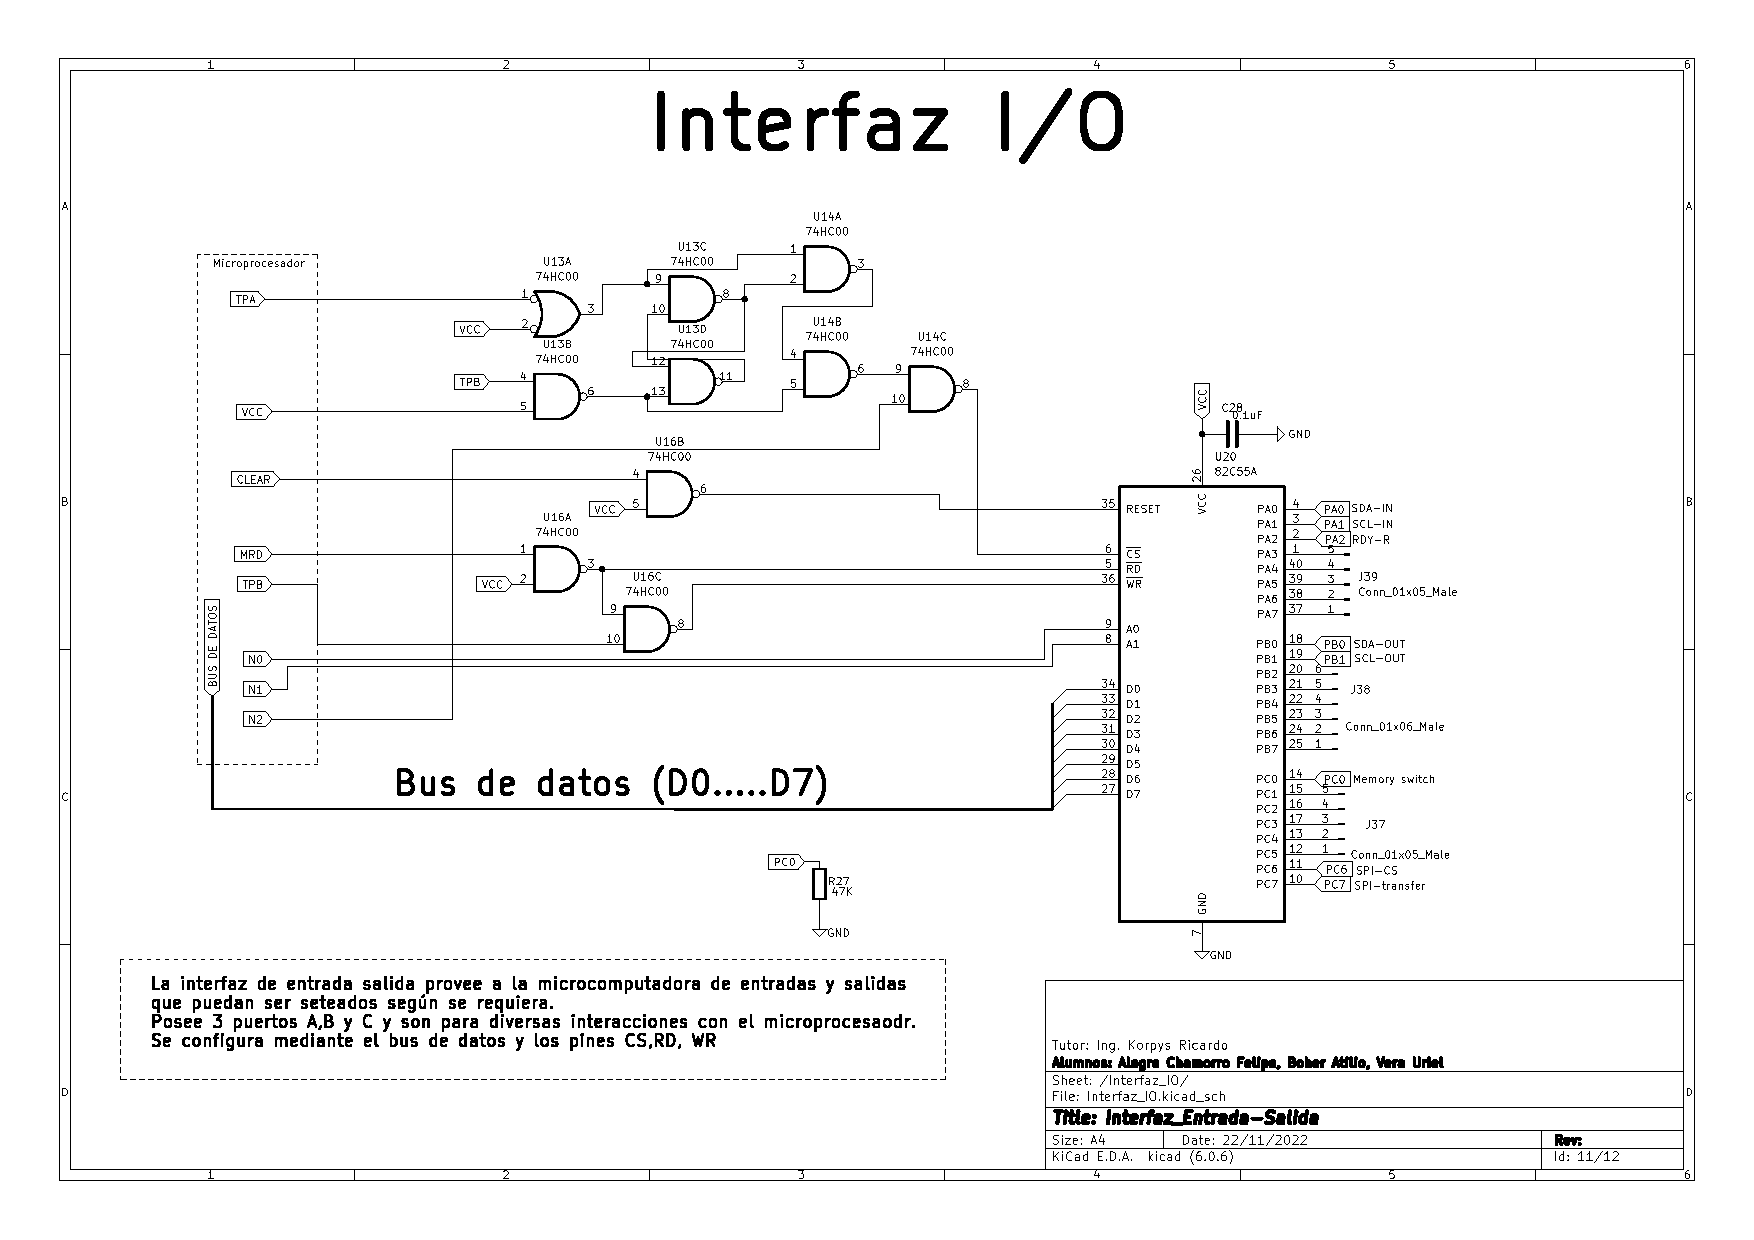
\includepdf[fitpaper, angle=90]{./imagenes/EsquematicosSF/Esquematico (11).pdf}
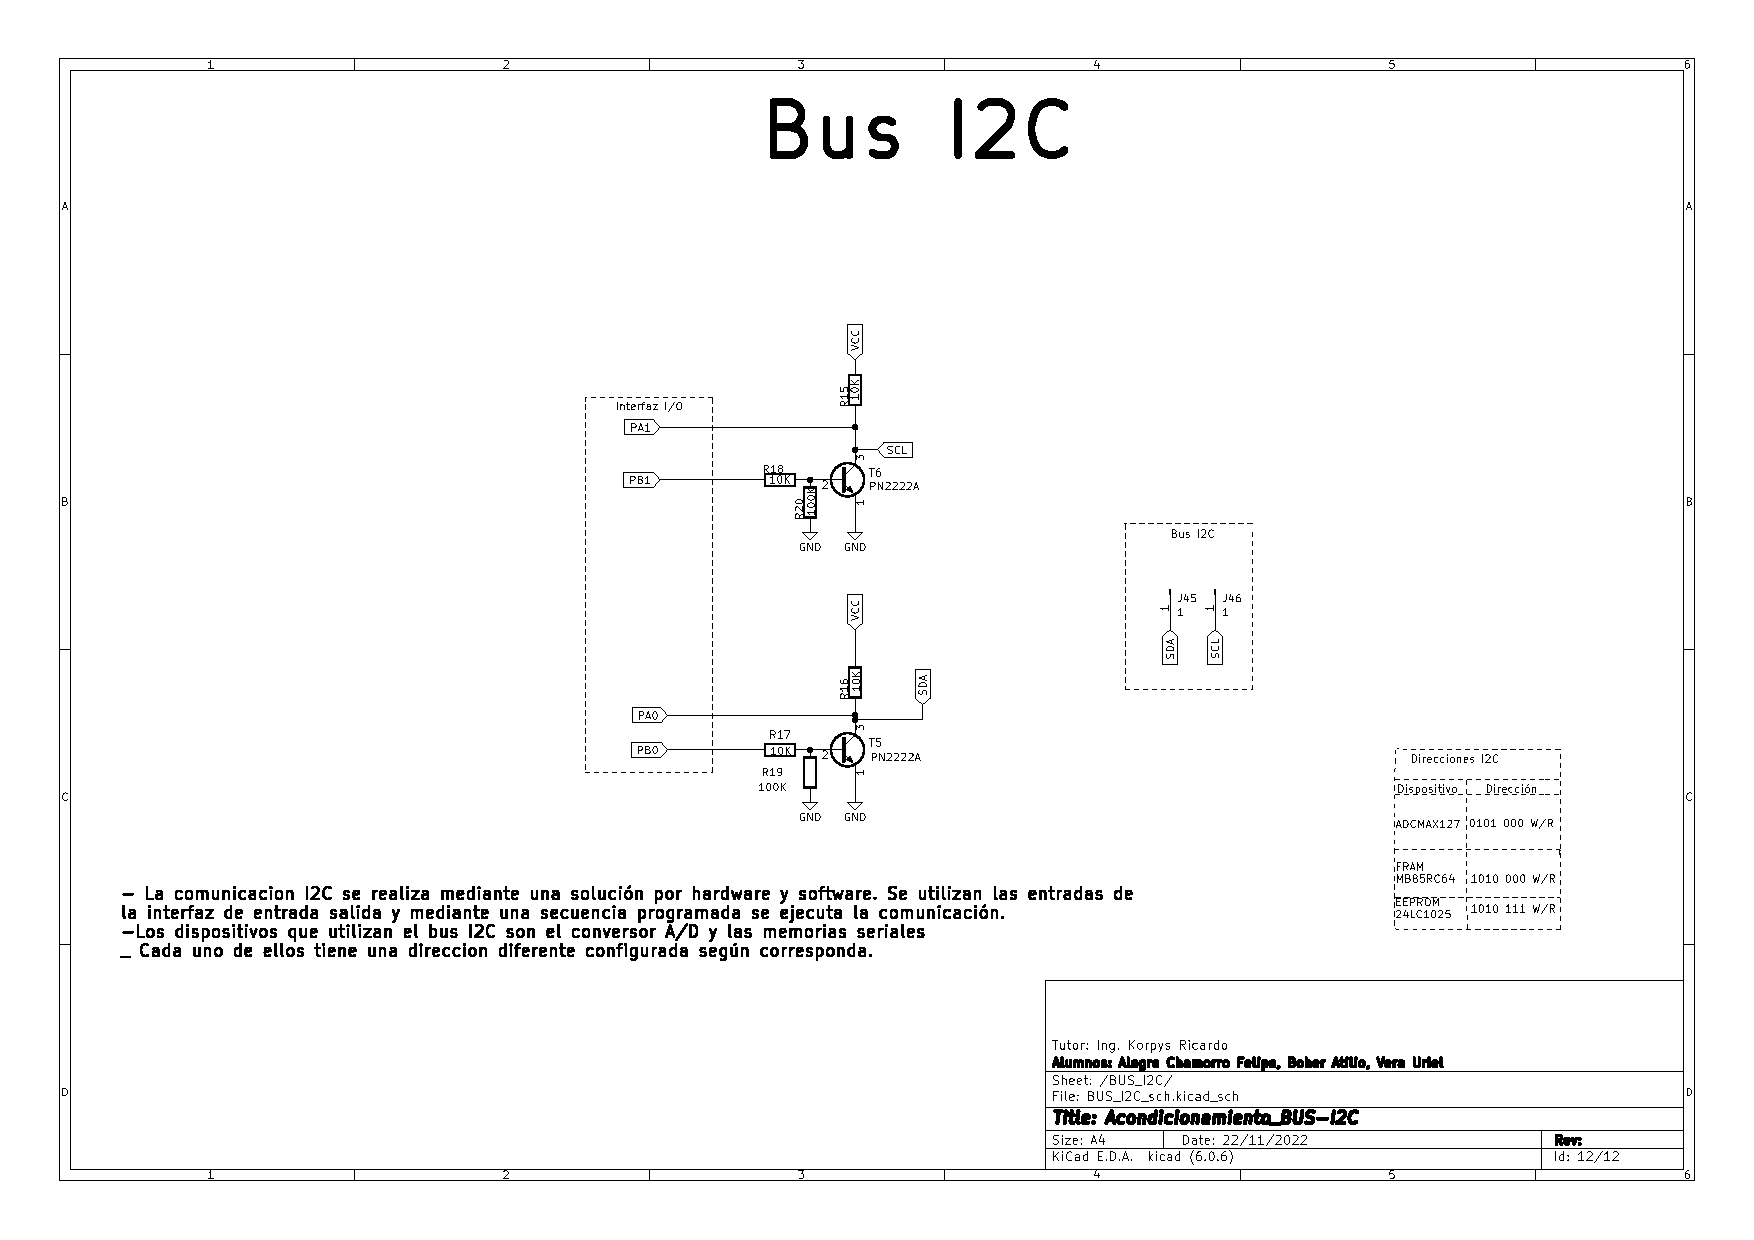
\includepdf[fitpaper, angle=90]{./imagenes/EsquematicosSF/Esquematico (12).pdf}
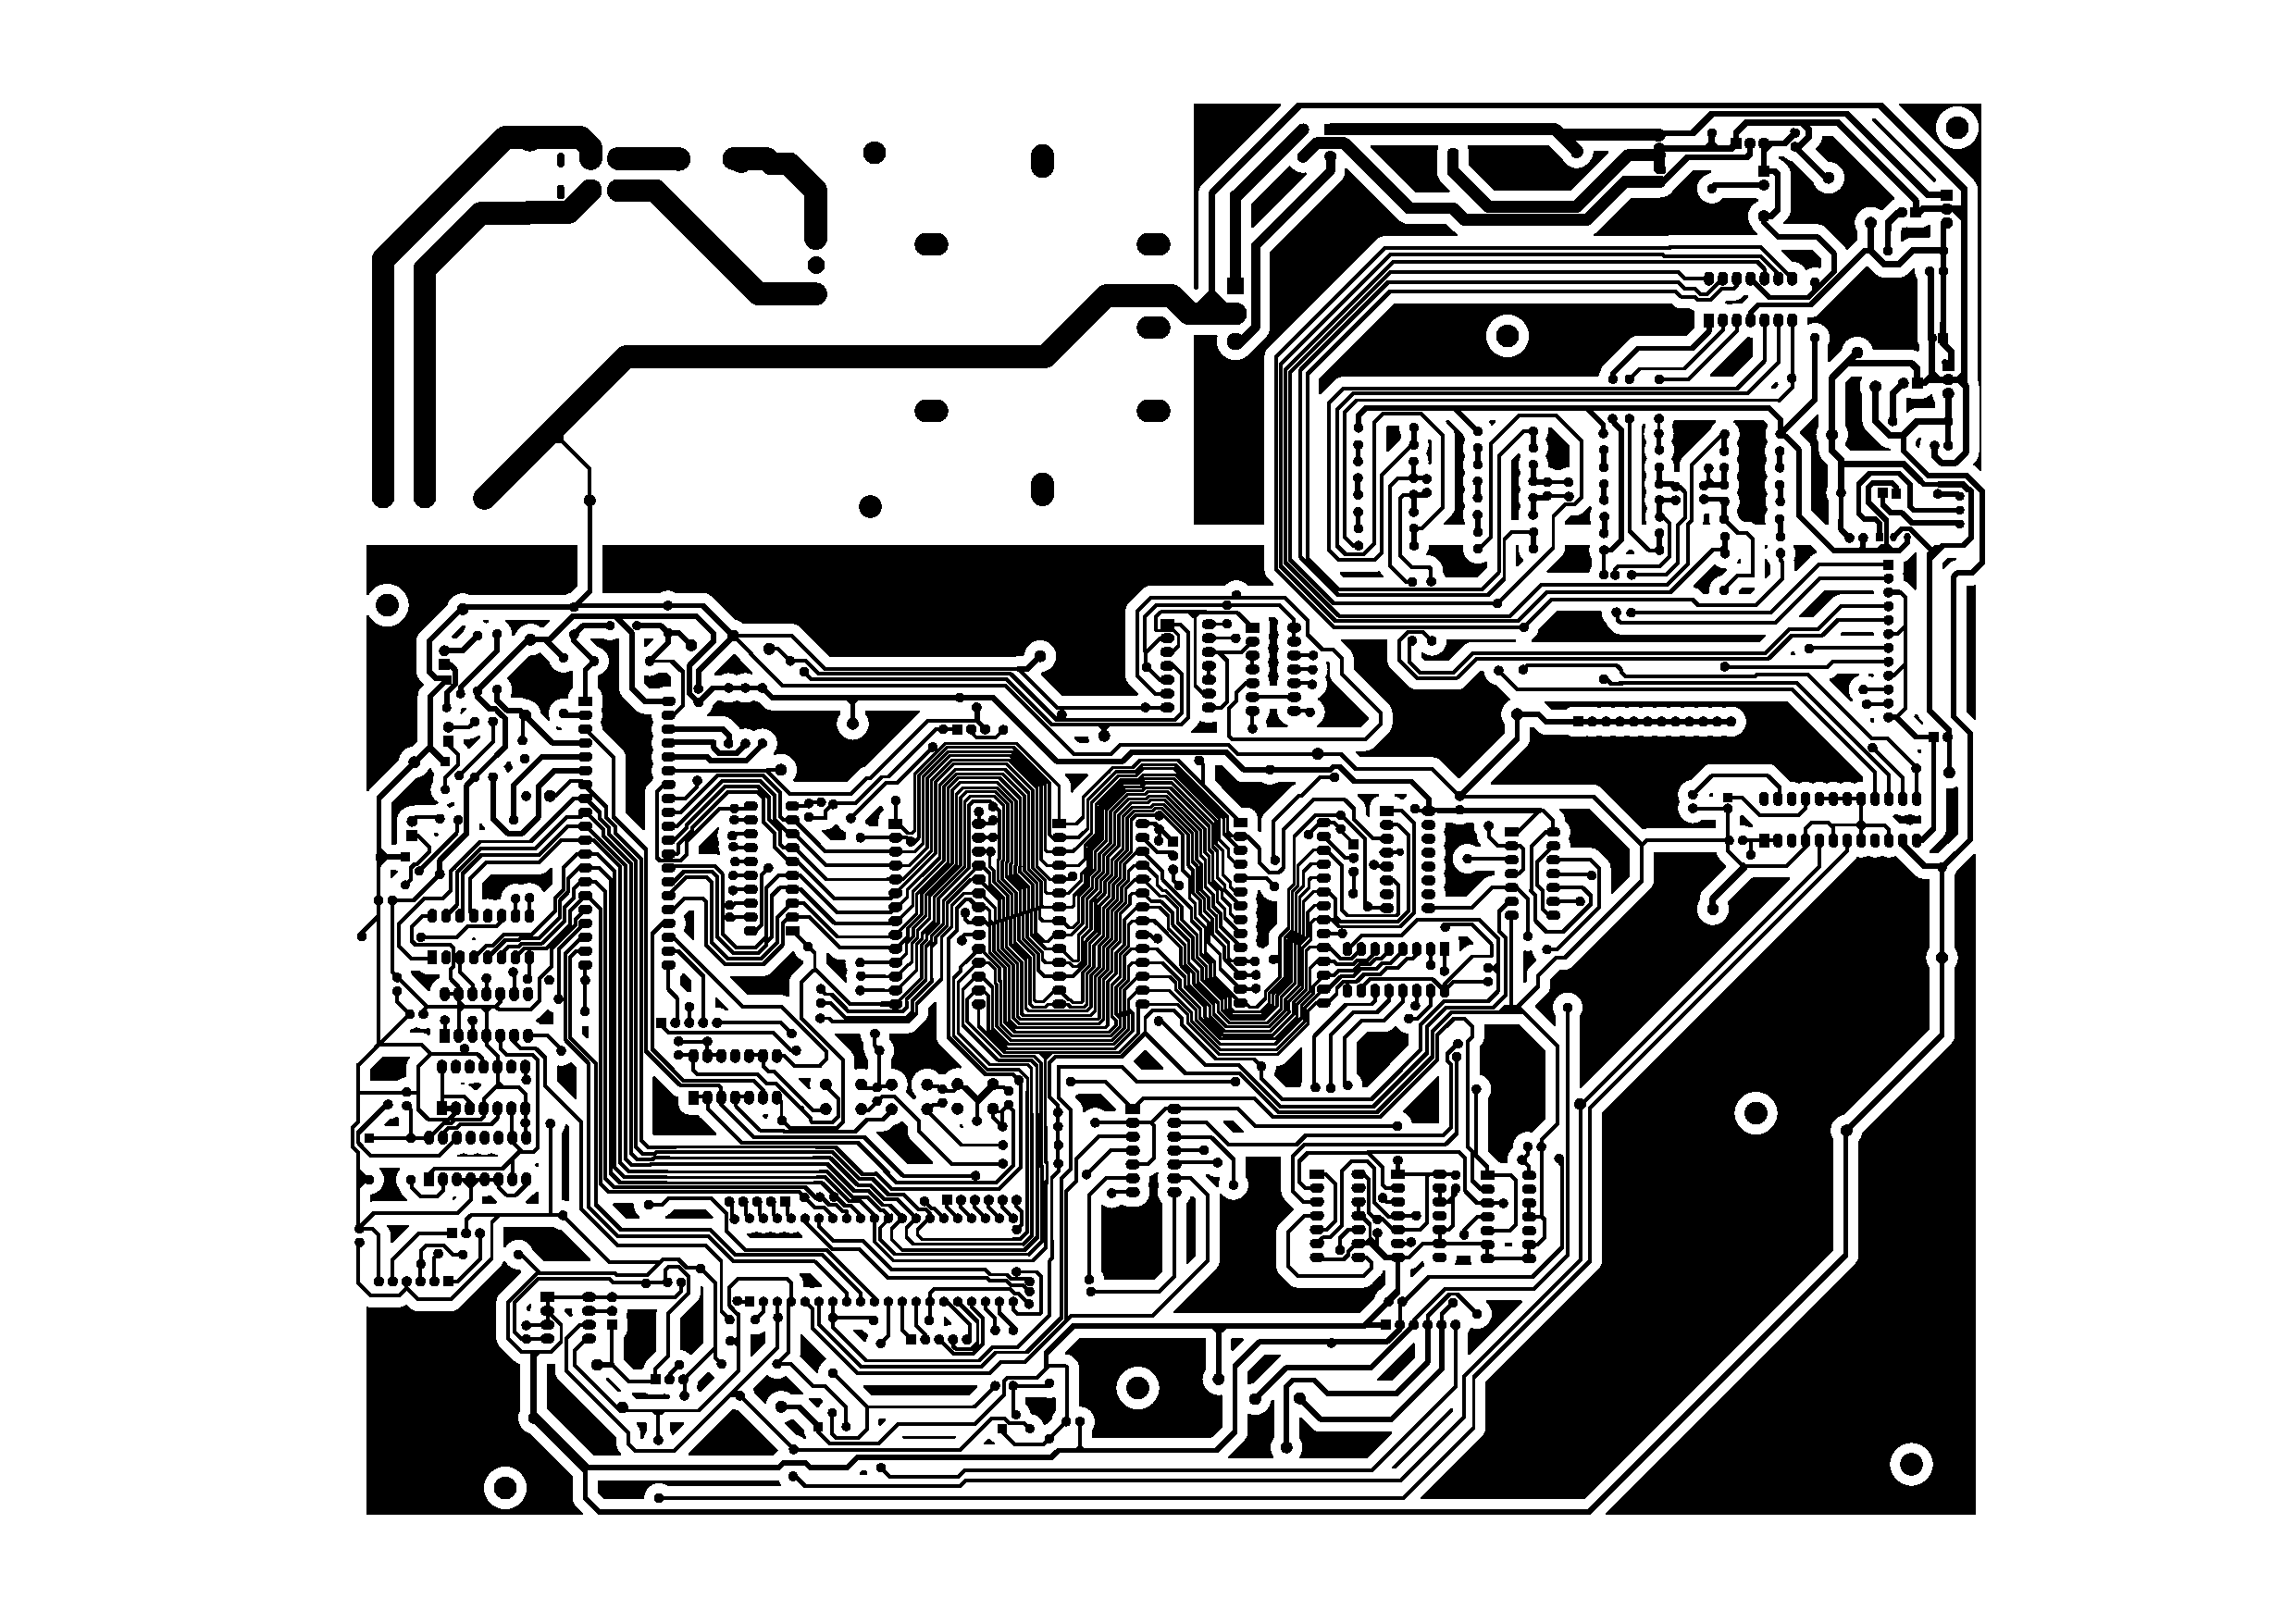
\includepdf[fitpaper]{./imagenes/EsquematicosSF/PCB_atras.pdf}
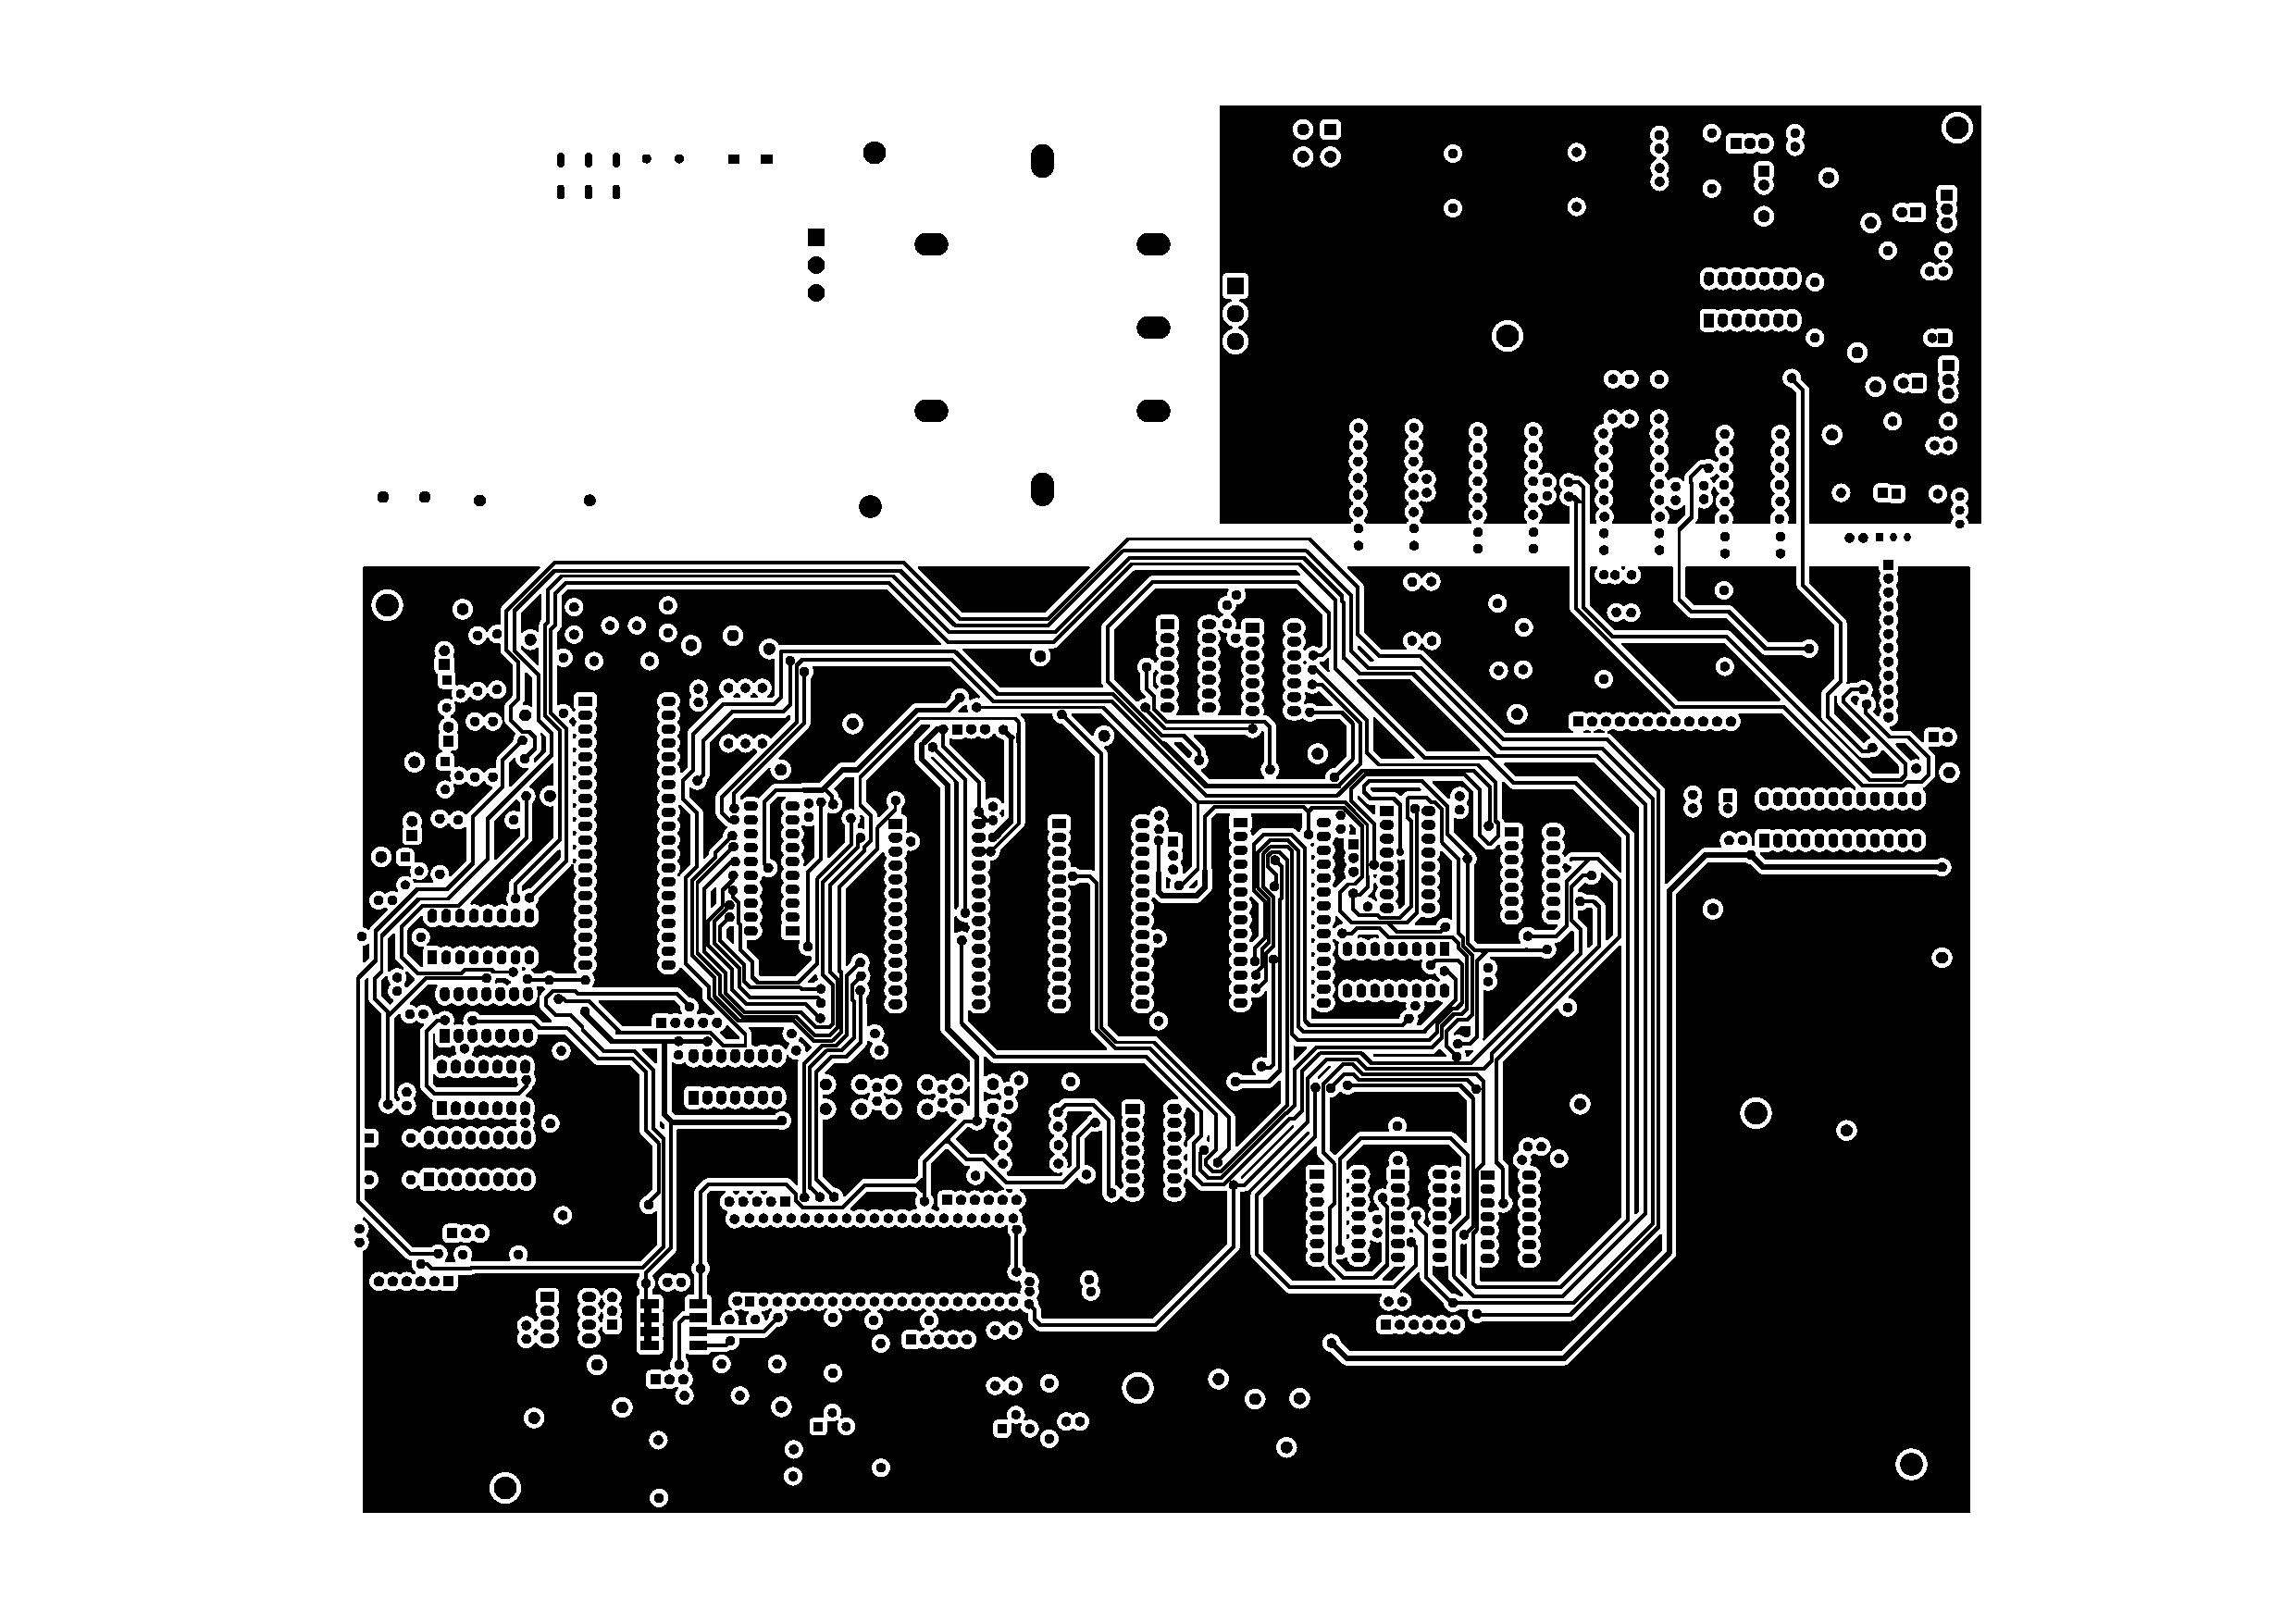
\includepdf[fitpaper]{./imagenes/EsquematicosSF/PCB_frente.pdf}
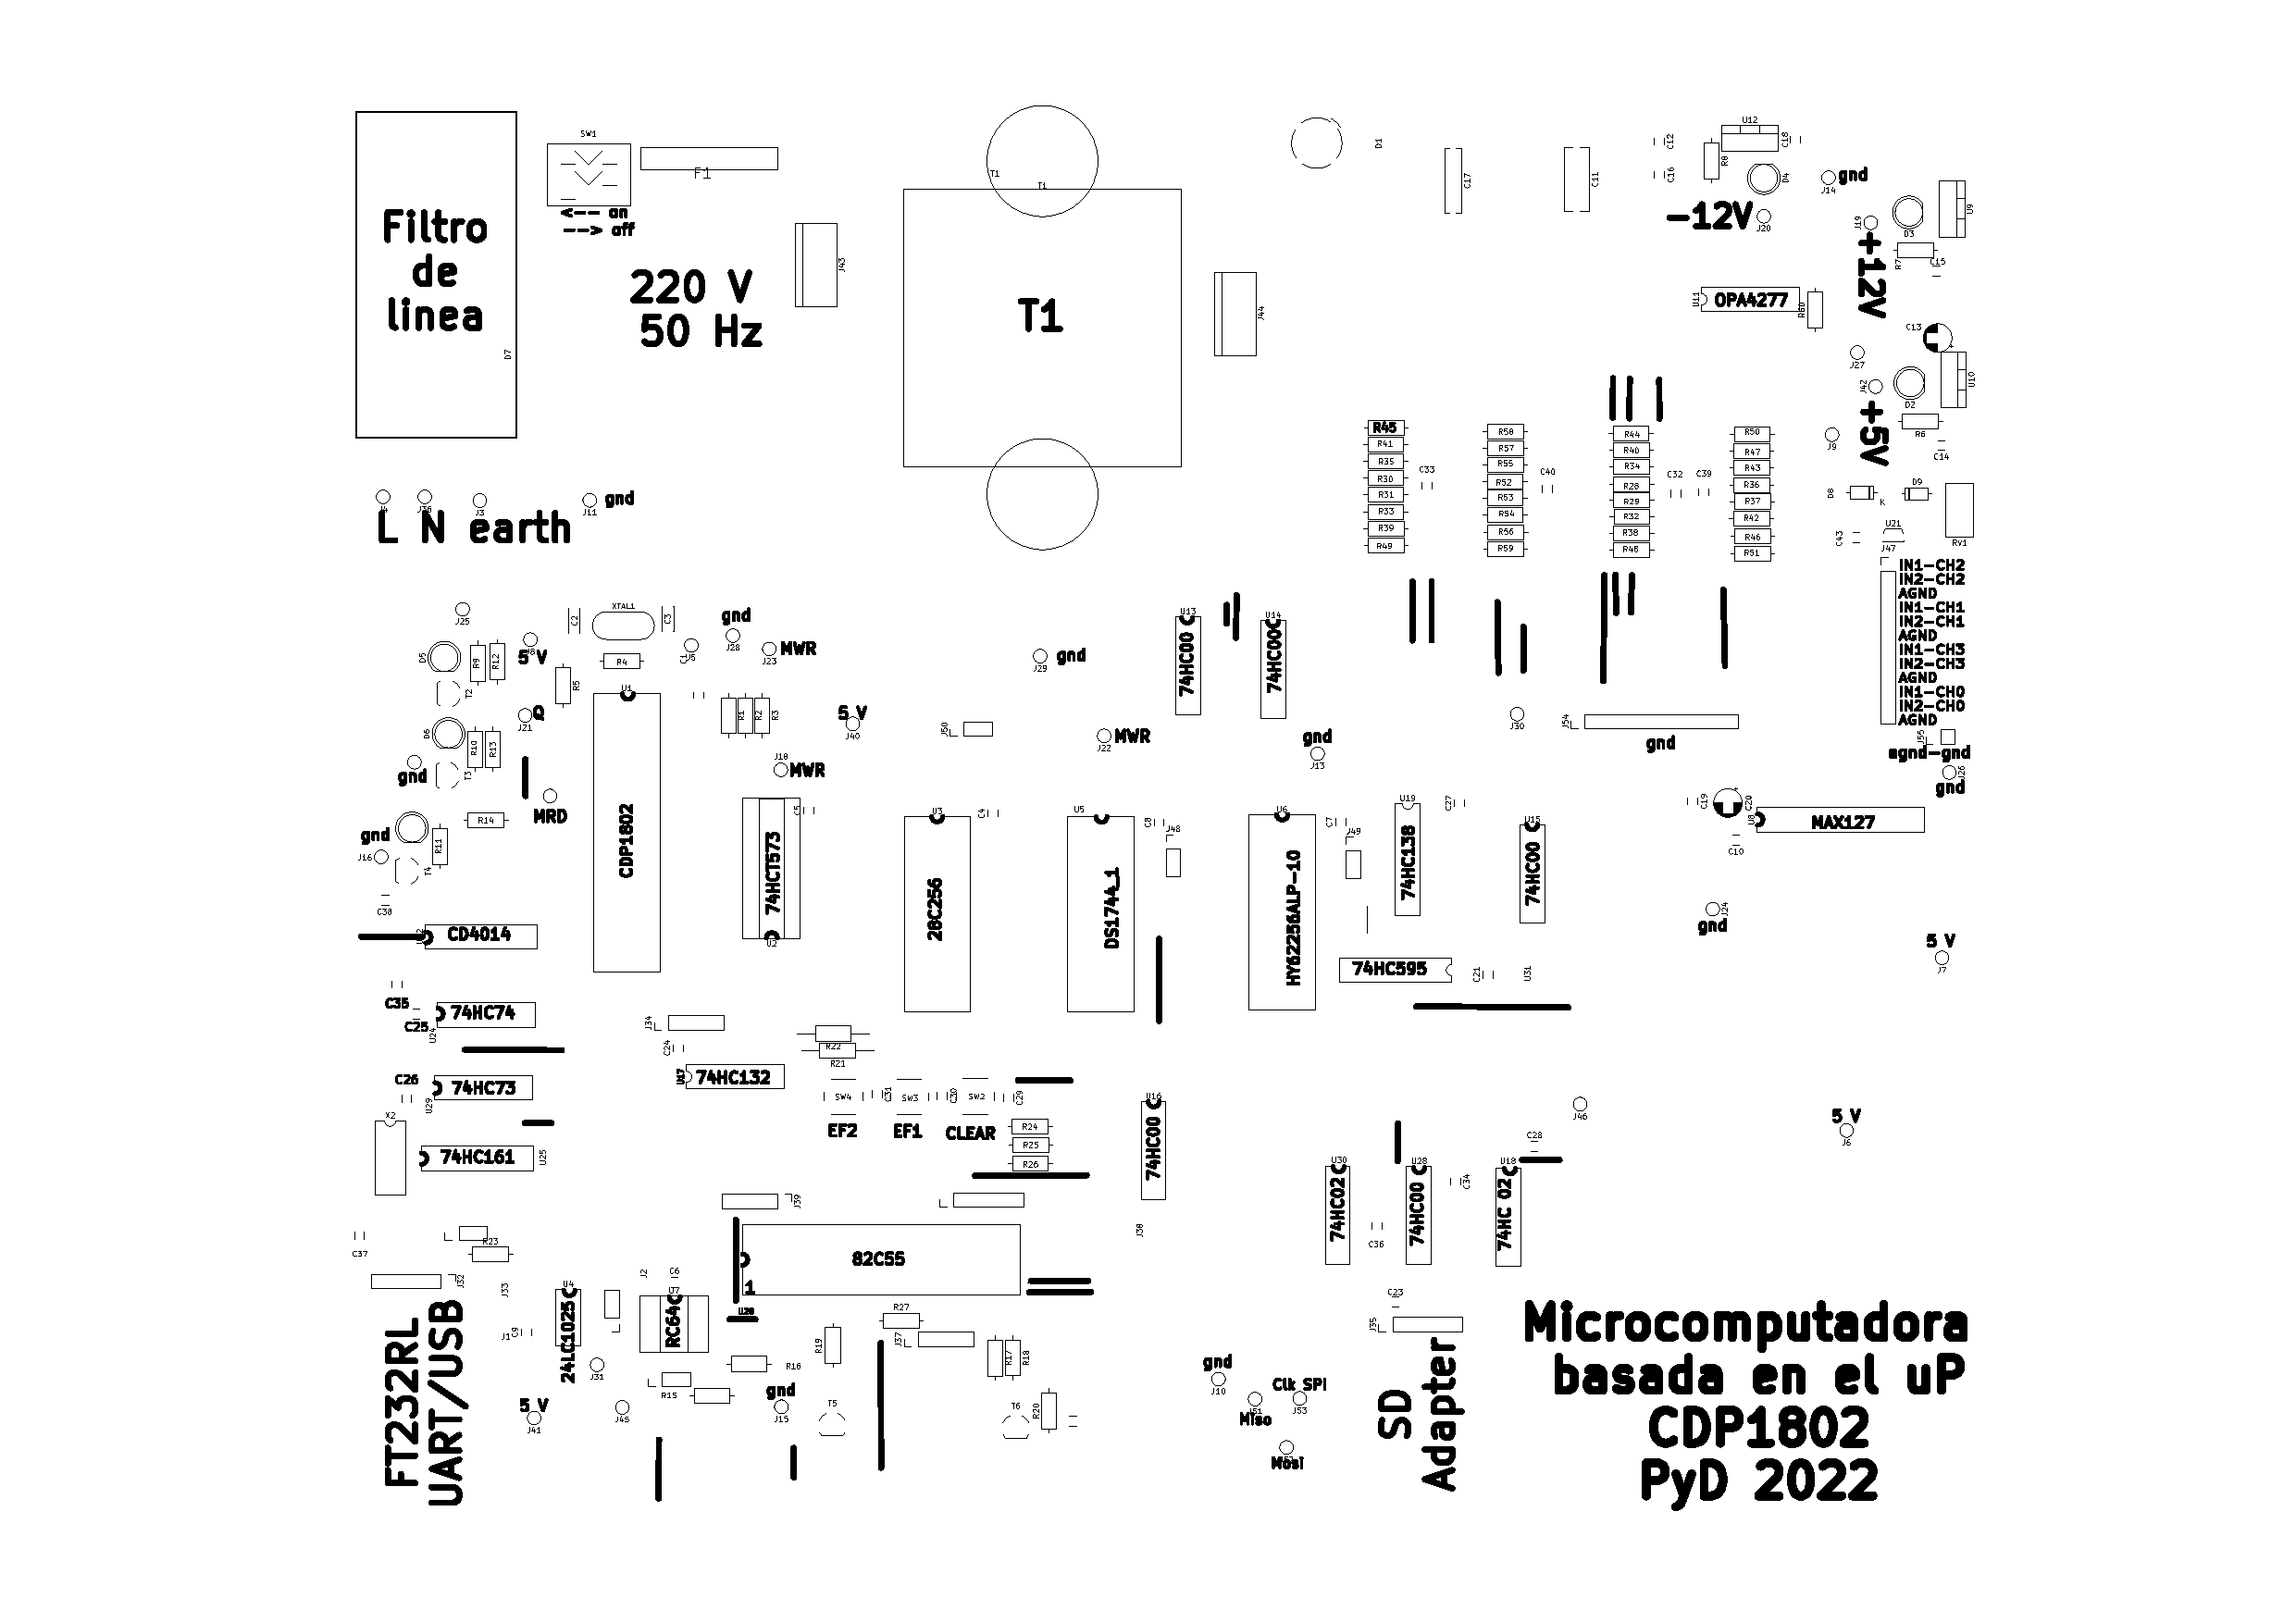
\includepdf[fitpaper]{./imagenes/EsquematicosSF/PCB_mascara.pdf}
%\input{apendices/B_archivo.tex}
%\input{apendices/reglamento_proyecto_electrico.tex}

\backmatter

%%%%%%%%%%%%%%%%%%%
\end{document}
%%%%%%%%%%%%%%%%%%%

% ----------------------------------------------
% Plantilla elaborada por Fabián Abarca Calderón
% ----------------------------------------------